\PassOptionsToPackage{hyphens}{url}
\documentclass[
  fontsize=12pt,
%  headings=openany,
%  headings=twolinechapter,
  twoside=semi,
  bibliography=totoc,
%  draft=true,
%  headsepline=true,
  DIV=11,
  ]{scrbook}

\setkomafont{publishers}{\large\itshape}

\usepackage[svgnames]{xcolor}

\colorlet{maincolour}{DarkSlateBlue}

\renewcommand\chapterlinesformat[3]{%
  \leavevmode\marginpar{\fontsize{96}{115}\selectfont\textcolor{maincolour}{#2}}%
  {\raggedleft #3\par}%
}

%\usepackage[autooneside=false]{scrlayer-scrpage}
%\pagestyle{scrheadings}
%\automark[section]{chapter}

\usepackage[autostyle]{csquotes}
\usepackage{polyglossia}
\setdefaultlanguage[variant=british]{english}

\begin{hyphenrules}[variant=british]{english}
  \hyphenation{Comp-Cert Veri-cert Comp-Cert-GSA Comp-Cert-SSA}
\end{hyphenrules}

\usepackage[
  backend=biber,
  backref=true,
  minbibnames=3,
  maxbibnames=9,
  maxcitenames=3,
  mincitenames=1,
  datamodel=acmdatamodel,
  style=acmauthoryear,
]{biblatex}

\addbibresource{thesis-refs.bib}
\addbibresource{ymh-refs.bib}

% For ACM author year citations
\newcommand{\bibliofont}{\normalfont\normalsize}
\renewcommand*{\bibfont}{\normalfont\normalsize}
\setlength\bibitemsep{\baselineskip}

%\usepackage{lineno}
%\linenumbers
\usepackage{amsmath}
\usepackage{amssymb}
\usepackage{amsthm}
\usepackage{amsfonts}
\usepackage{textcomp}

\usepackage{verbatim}

\usepackage{accents}
\usepackage{enumitem}
\usepackage{soul}
\usepackage{subcaption}

\usepackage{pgfplotstable}
\usepackage{pgfplots}
\pgfplotsset{compat=1.18}

\usepackage{tikz-timing}
\usepackage{tikz}
\usetikzlibrary{arrows,arrows.meta,shapes,snakes,automata,backgrounds,petri,%
                decorations.pathreplacing,calligraphy,patterns,%
                patterns.meta,pgfplots.groupplots,positioning,shapes.geometric,%
                fit,tikzmark}

\usepackage{mathpartir}
\usepackage{multirow}
\usepackage{booktabs}
\usepackage{tikzpagenodes}
\usepackage{microtype}

\usepackage{setspace}
\onehalfspacing

\usepackage{minted}
\setminted{fontsize=\small}
\usemintedstyle{manni}

\usepackage[colorlinks=true,pdfa]{hyperref}
\hypersetup{allcolors=maincolour}

\usepackage[acronym,index,symbols,xindy,nomain]{glossaries-extra}
\usepackage{glossary-bookindex}
\setabbreviationstyle[acronym]{long-short}
\makeatletter
\newcommand*{\glsplainhyperlink}[2]{%
    \begingroup%
      \hypersetup{hidelinks}%
      \hyperlink{#1}{#2}%
    \endgroup%
}
\let\@glslink\glsplainhyperlink
\makeatother
\makeglossaries

\usepackage{cleveref}

\usepackage{ymh-macros}

%% https://tex.stackexchange.com/a/535849
\usepackage{hyperxmp}
%\usepackage{embedfile}

%\usepackage{uni-titlepage}
%\TitlePageStyle{UKoLa}

\subject{PhD Thesis}
\title{Formal Verification of High-Level Synthesis}
\author{Yann Herklotz Grave}

\publishers{Supervised by \\ Dr John Wickerson}

\makeatletter
\newcommand\@titlefooter{Submitted in part fulfilment of the requirements for
the degree of Doctor of Philosophy in Electrical and Electronic Engineering of
Imperial College London.}
\makeatother

%\university{Imperial College London}

\hypersetup{%
    pdflang=la,
    pdfapart=3, %set to 1 for PDF/A-1
    pdfaconformance=B
}

%\embedfile[afrelationship={/Source},ucfilespec={\jobname.tex},mimetype={application/x-tex}]{\jobname.tex}

%Create an OutputIntent in order to correctly specify colours
\immediate\pdfobj stream attr{/N 3} file{sRGBIEC1966-2.1.icm}
\pdfcatalog{%
  /OutputIntents [
    <<
      /Type /OutputIntent
      /S /GTS_PDFA1
      /DestOutputProfile \the\pdflastobj\space 0 R
      /OutputConditionIdentifier (sRGB)
      /Info (sRGB)
    >>
  ]
}

% https://tex.stackexchange.com/a/474336
\pdfvariable omitcidset=1

\newacronym{SSA}{SSA}{static single assignment}
\newacronym{GSA}{GSA}{gated-SSA}
\newacronym{HDL}{HDL}{hardware description language}
\newacronym{HLS}{HLS}{high-level synthesis}
\newacronym{FPGA}{FPGA}{field-programmable gate array}
\newacronym{DFG}{DFG}{data-flow graph}
\newacronym{CFG}{CFG}{control-flow graph}
\newacronym{CDFG}{CDFG}{control- and data-flow graph}
\newacronym{SDC}{SDC}{system of difference constraints}
\newacronym{CNF}{CNF}{conjunctive normal form}
\newacronym{SAT}{SAT}{satisfiability}
\newacronym{SMT}{SMT}{satisfiability modulo theories}
\newacronym{DSP}{DSP}{digital signal processor}
\newacronym{ITP}{ITP}{interactive theorem prover}
\newacronym{FSMD}{FSMD}{finite-state machine with data path}
\newacronym{II}{II}{initiation interval}
\newacronym{ASAP}{ASAP}{as soon as possible}
\newacronym{ALAP}{ALAP}{as late as possible}
\newacronym{LUT}{LUT}{look-up table}
\newacronym{MRT}{MRT}{modulo reservation table}
\newacronym{LSQ}{LSQ}{load-store queue}
\newacronym{BRAM}{BRAM}{block random access memory}
\newacronym{ASIC}{ASIC}{application-specific integrated circuit}
\newacronym{IR}{IR}{intermediate representation}
\newacronym{DSL}{DSL}{domain-specific language}
\newacronym{CPU}{CPU}{central processing unit}
\newacronym{GPU}{GPU}{graphics processing unit}
\newacronym{IPcore}{IP core}{intellectual property core}
\newacronym{AST}{AST}{abstract syntax tree}
\newacronym{ILP}{ILP}{integer linear programming}
\newacronym{LP}{LP}{linear programming}
\newglossaryentry{RTL}{type=\acronymtype, name={\textsc{Rtl}},
  description={register transfer language}, first={register transfer language (\textsc{Rtl})}}

\newterm[name={\enquote{plus} forward simulation},sort=plusforwardsimulation]{plus-forward-simulation}
\newterm[name={\enquote{star} forward simulation},sort=starforwardsimulation]{star-forward-simulation}
\newterm{CompCert}
\newterm{translation validation}
\newterm{data flow}
\newterm{control flow}
\newterm{data path}
\newterm{control logic}
\newterm{basic block}
\newterm{superblock}
\newterm{hyperblock}
\newterm{predicated instruction}
\newterm{scheduling}
\newterm[see={[see also]scheduling}]{list scheduling}
\newterm[see={[see also]{hyperblock,scheduling}}]{hyperblock scheduling}
\newterm[see={[see also]{superblock,scheduling}}]{superblock scheduling}
\newterm{static scheduling}
\newterm{dynamic scheduling}
\newterm{operation chaining}

\glsxtrnewsymbol[description={variable defining the time step of an
  operation}]{scheduling variable}{\ensuremath{\mathrm{sv}}}

%\newterm

\includeonly{%
 % titlepage,
 % copyright-assignment,
 % abstract,
 % acknowledgements,
 % chapters/1-introduction,
 chapters/2-background,
 % chapters/3-introduction-to-vericert,
 % chapters/4-trusted-computing-base,
 % chapters/5-hyperblock-scheduling,
 % chapters/6-hardware-generation,
 % chapters/7-evaluation,
 % chapters/8-conclusion,
}

\begin{document}

\makeatletter
{\singlespacing
\begin{titlepage}
  \centering
  {\usekomafont{subject}\@subject\par}
  \vspace{4\baselineskip}
  {\usekomafont{title}\huge\@title\par}
%  \vspace{2\baselineskip}
%  {\Large \@subtitle\par}
  \vspace{6\baselineskip}
  {\usekomafont{author}\@author\par}
  \vspace{2\baselineskip}
  {\usekomafont{date}\@date\par}
  \vspace{6\baselineskip}
  {\usekomafont{publishers}\@publishers\par}
  \vfill
  {\@titlefooter\par}
\end{titlepage}}
\makeatother

%%% Local Variables:
%%% mode: latex
%%% TeX-master: "thesis"
%%% TeX-engine: luatex
%%% End:


\addcontentsline{toc}{chapter}{Copyright Assignment}

\thispagestyle{empty}

\noindent\begin{tabular}{ll}
  \textbf{Supervisor:} & Dr John Wickerson\\
  \textbf{Internal Examiner:} & Prof George Constantinides\\
  \textbf{External Examiner:} & Prof Xavier Leroy\\
\end{tabular}

\vfill

\makeatletter
\noindent Copyright \copyright{} \the\year{} \@author.
\makeatother

\vspace{5\baselineskip}

\noindent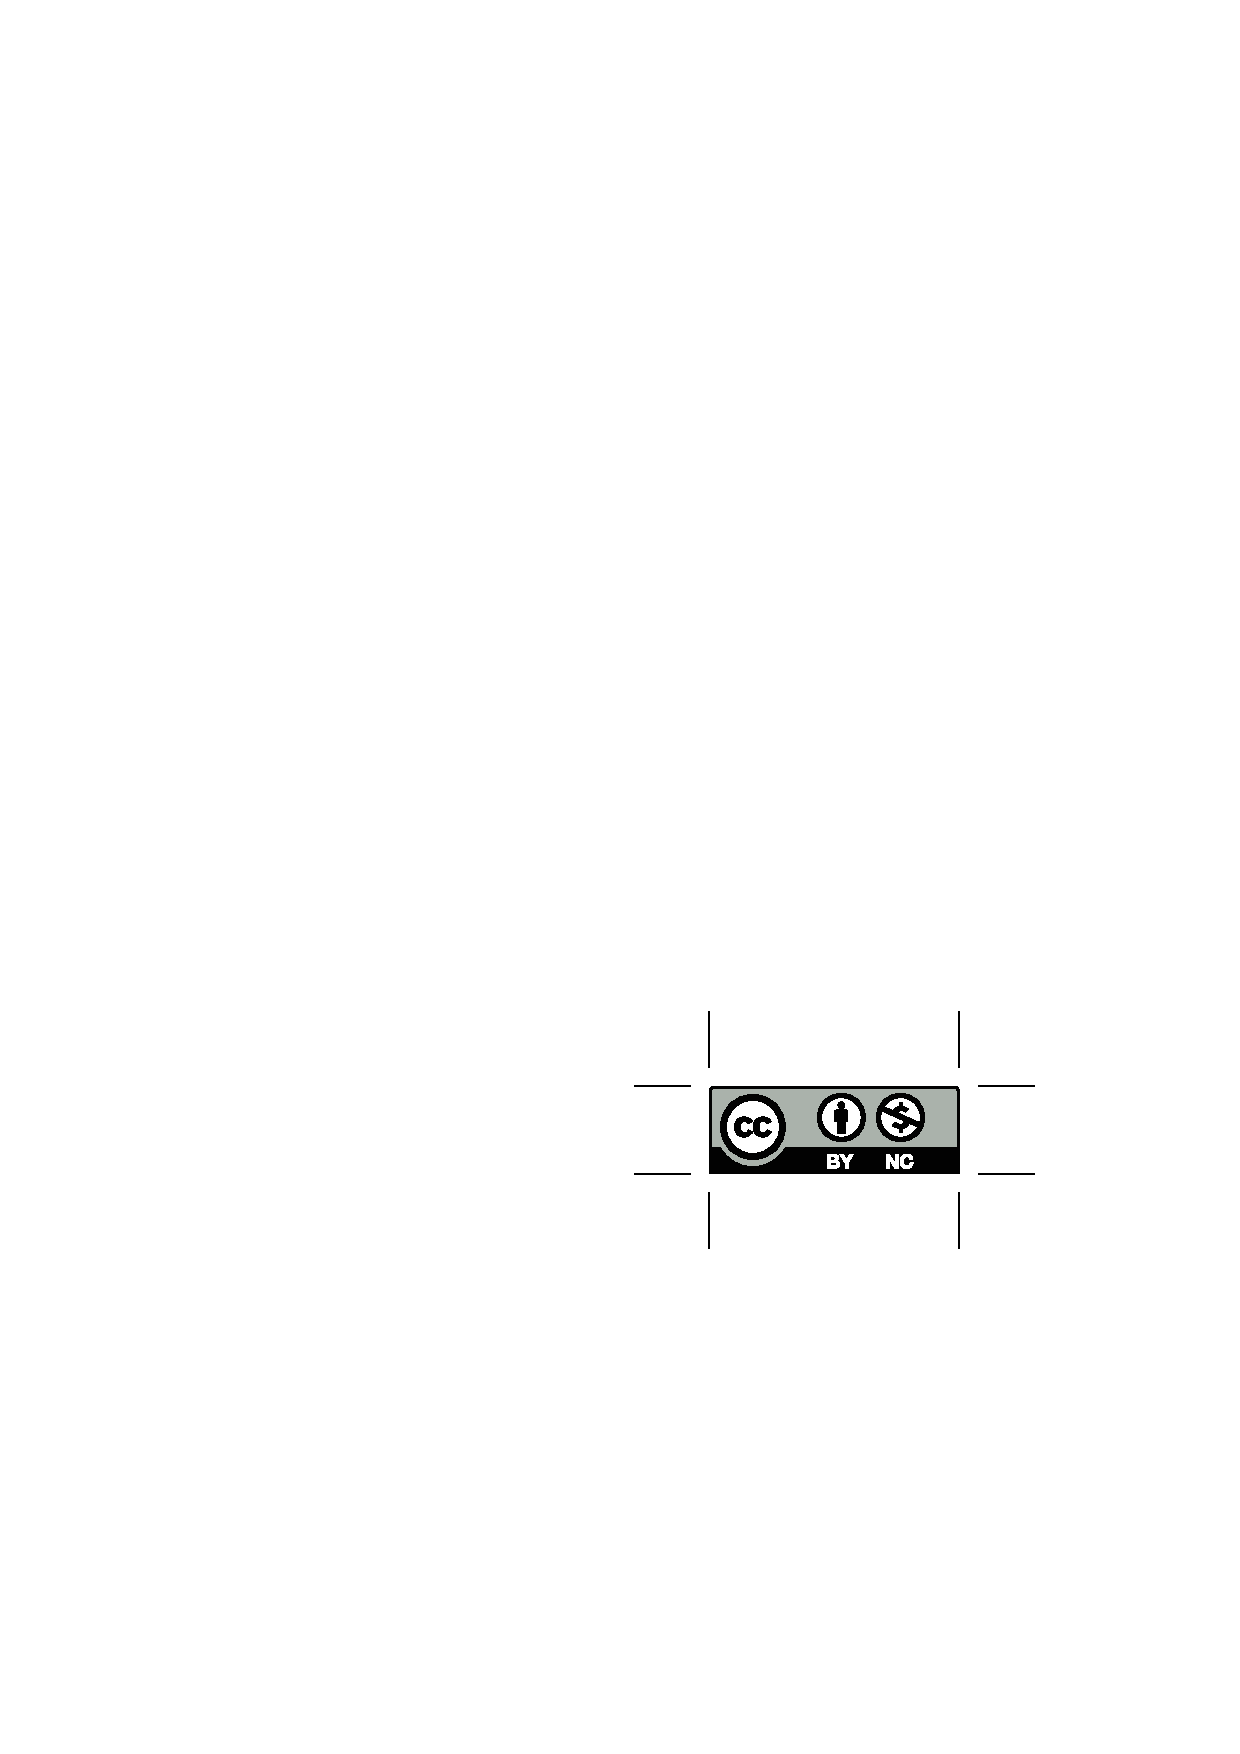
\includegraphics{assets/cc-by-nc}\hfill%
\raisebox{1\baselineskip}{\begin{minipage}[c]{0.65\linewidth} The copyright of
    this dissertation rests with the author. Unless otherwise indicated, its
    contents are licensed under a
    \href{https://creativecommons.org/licenses/by-nc/4.0/}{Creative Commons
      Attribution-NonCommercial 4.0 International Licence (CC BY-NC)}.
\end{minipage}}

%Under this licence, you may copy and redistribute the material in any medium or
%format. You may also create and distribute modified versions of the work. This
%is on the condition that: you credit the author and do not use it, or any
%derivative works, for a commercial purpose.
%
%When reusing or sharing this work, ensure you make the licence terms clear to
%others by naming the licence and linking to the licence text. Where a work has
%been adapted, you should indicate that the work has been changed and describe
%those changes.
%
%Please seek permission from the copyright holder for uses of this work that are
%not included in this licence or permitted under UK Copyright Law.

%%% Local Variables:
%%% mode: latex
%%% TeX-master: "thesis"
%%% TeX-engine: luatex
%%% End:


\addchap{Abstract}

%%% Local Variables:
%%% mode: latex
%%% TeX-master: "thesis"
%%% End:


\addchap{Acknowledgements}

%%% Local Variables:
%%% mode: latex
%%% TeX-master: "thesis"
%%% TeX-engine: luatex
%%% End:


\tableofcontents

\listoffigures

\listoftables

\printglossary[type=acronym,nonumberlist]

\glsresetall

\chapter{Introduction}%
\label{sec:introduction}

%% Motivation for why HLS might be needed

% \JW{A few high-level comments: \begin{enumerate} \item Create more tension
%   from the start by making the reader doubt whether existing HLS tools are
%   trustworthy. \item The intro currently draws quite a bit of motivation from
%   Lidbury et al. 2015, but we should also now lean on our FPGA submission
%   too. \item I wonder whether the paragraph `To mitigate the problems...'
%   should be demoted to a `related work' discussion (perhaps as a subsection
%   towards the end of the introduction). It outlines (and nicely dismisses)
%   some existing attempts to tackle the problem, which is certainly useful
%   motivation for your work, especially for readers already familiar with HLS,
%   but I feel that it's not really on the critical path for understanding the
%   paper.\end{enumerate}}

% \NR{I couldn't have subsections in comments so I have appended my writing to
% the bottom of this file.}\YH{The original intro is in the archive, we can
% maybe merge them in the future a bit.}

Latency, throughput, and energy efficiency are become increasingly important,
leading to more custom hardware accelerators being designed for numerous
applications.  Alas, designing these accelerators can be a tedious and
error-prone process, especially when using a \gls{HDL} such as Verilog, which
operates at the register transfer level, where the hardware needs to be laid out
manually.  As the complexity of these hardware designs increases, designing
hardware at this level can hamper productivity.  An increasingly attractive
alternative is \emph{\gls{HLS}}, where hardware designs are automatically
compiled from software written in a high-level language like C.  Modern
\gls{HLS} tools such as \legup{}~\cite{canis11_legup}, Vitis
HLS~\cite{amd23_vitis_high_synth}, Intel i++~\cite{intel_hls}, Stratus
HLS~\cite{roane23_autom_hw_sw_co_desig} and Bambu HLS~\cite{bambu_hls} promise
designs with comparable performance and energy-efficiency to those hand-written
in an \gls{HDL}~\cite{homsirikamol+14, silexicahlshdl, 7818341}.  They also
promise to reduce the time taken to design hardware and make the design more
flexible so that different architectures can be explored.

\gls{HLS} should ideally also benefit verification of the functionality of the
hardware design.  Checking the functionality of designs written using
\glspl{HDL} often cannot be fully verified because of their size and the
additional detail that needs to be taken into account.  \gls{HLS} moves the
functional verification problem to a higher-level, allowing for a much deeper
understanding about the functional behaviour of the design.  A recent survey by
\textcite{lahti19_are_we_there_yet} describes that verification is still a
time-consuming part of the design process though, even with the use of
\gls{HLS}, however, that in general it still reduced the verification effort by
half.  Most papers that were surveyed did not mention verification of designs
though and it therefore still remains an underexplored area in \gls{HLS}
research.

% \YH{TODO: Talk about the history of HLS to motivate it better.}

\paragraph{Can you trust your high-level synthesis tool?}

Indeed, there are reasons to doubt that \gls{HLS} tools actually \emph{do}
always preserve equivalence, increasing the chance of there being exploitable
hardware faults in the resulting accelerator.  Some of these reasons are
general: \gls{HLS} tools are large pieces of software, they perform a series of
complex analyses and transformations, and the \gls{HDL} output they produce has
superficial syntactic similarities to a software language but a subtly different
semantics.  Other reasons are more specific: for instance, Vivado HLS has been
shown to apply pipelining optimisations
incorrectly\footnote{\url{https://bit.ly/vivado-hls-pipeline-bug}\YH{Need to
  find the link again}} or to silently generate wrong code should the programmer
stray outside the fragment of C that it
supports.\footnote{\url{https://support.xilinx.com/s/question/0D52E00006hpMZSSA2/pointer-synthesis-in-vivado-hls-v201}}\textsuperscript{,}\footnote{\url{https://docs.xilinx.com/r/en-US/ug1399-vitis-hls/Pointer-Limitations}}
Meanwhile, \textcite{lidbury15_many_core_compil_fuzzin} had to abandon their
attempt to fuzz-test Altera's (now Intel's) OpenCL compiler since it ``either
crashed or emitted an internal compiler error'' on so many of their test inputs.
More recently, \textcite{herklotz21_empir_study_reliab_high_level_synth_tools}
fuzz-tested three commercial \gls{HLS} tools using
Csmith~\cite{yang11_findin_under_bugs_c_compil}, and despite restricting the
generated programs to the C fragment explicitly supported by all the tools, they
still found that on average 2.5\% of test-cases were compiled to designs that
behaved incorrectly.

Compared to software, it is necessary to ensure that hardware functions as it is
supposed to, because once the hardware has been taped-out into an \gls{ASIC},
there is no way to properly fix the issue except to work around it in software.
This may come at a great cost compared to fixing the issue in hardware itself on
both the energy usage and the performance of the
system~\cite{herzog21_price_meltd_spect,bowen20_perfor_cost_softw_based_secur_mitig}.
These hardware faults can also often be exploited and can be hard to detect,
even using state-of-the-art hardware verification
methodologies~\cite{dessouky19_hardf}, sometimes because the correctness
properties themselves can be hard to express, or because the state-space that
needs to be explored by the tools is too large.

\paragraph{Existing workarounds}

Aware of the reliability shortcomings of \gls{HLS} tools, hardware designers
routinely check the generated hardware for functional correctness.  This is
commonly done by simulating the generated design against a large test-bench.
But unless the test-bench covers all inputs exhaustively -- which is often
infeasible -- there is a risk that bugs remain.

One alternative is to use
\emph{\gls{translation-validation}}~\cite{pnueli98_trans} to prove equivalence
between the input program and the output design. \Gls{translation-validation}
has been successfully applied to several \gls{HLS}
optimisations~\cite{kim04_autom_fsmd,
  karfa06_formal_verif_method_sched_high_synth,
  chouksey20_verif_sched_condit_behav_high_level_synth,
  banerjee14_verif_code_motion_techn_using_value_propag,
  chouksey19_trans_valid_code_motion_trans_invol_loops}.  Nevertheless, it is an
expensive task, especially for large designs, and it must be repeated every time
the compiler is invoked.  For example, the translation validation for Catapult
C~\cite{mentor20_catap_high_level_synth} may require several rounds of expert
`adjustments'~\cite[p.~3]{slec_whitepaper} to the input C program before
validation succeeds. And even when it succeeds, translation validation does not
provide watertight guarantees unless the validator itself has been mechanically
proven correct~\cite[e.g.][]{tristan08_formal_verif_trans_valid}, which has not
been the case in \gls{HLS} tools to date.

%\JW{Having nuanced our discussion of TV above, I feel like the text below
%belongs more in a `future directions' paragraph at the end of the paper than in
%an `existing workarounds' section.} Nevertheless translation validation has
%many benefits in a mechanically verified setting as well to simplify the proofs
%to depend less on the exact implementation of the optimisation.  It has also
%already been used to prove certain passes in \compcert{} correct.  The main
%issue with the translation validation methods applied in HLS tools normally is
%that they \NR{\sout{try and}} generalise over all optimisations that are
%performed and \NR{\sout{try to}} compare the generated hardware directly to the
%high-level input. \NR{The word input used here again.}  However, verification
%requires optimisations to be proven correct incrementally and separately,
%making translation validation more viable.  By proving specific optimisations
%with a constraint on the kinds of transformations it can perform, it is
%possible to write a verified validator that is also believed to be complete and
%should not fail on valid transformations unless bugs are present.

Our position is that none of the above workarounds are necessary if the HLS tool
can simply be trusted to work correctly.  The thesis for this dissertation is
therefore the following.

\begin{samepage}
  \begin{quote}
    \textbf{Thesis}\quad An optimising high-level synthesis tool can be proven
    correct using an interactive theorem prover, guaranteeing the correctness of
    the hardware while also remaining practical and efficient.
  \end{quote}
\end{samepage}

% \NR{Perhaps, we can add something like: `... and our efforts are the first
% step towards building this trust within HLS
% tools.'.} %JW: I think that would be over-egging the cake.

\paragraph{Our solution}
We have designed a new HLS tool in the Coq theorem prover and proved that any
output design it produces always has the same behaviour as its input program.
Our tool, called \vericert{}, is automatically extracted to an OCaml program
from Coq, which ensures that the object of the proof is the same as the
implementation of the tool.  \vericert{} is built by extending the \compcert{}
verified C compiler~\cite{leroy09_formal_verif_realis_compil} with a new
hardware-specific intermediate language and a Verilog back end.  It supports
many C constructs, including integer operations, function calls (which are all
inlined), local arrays, structs, unions, and general control-flow statements,
but currently excludes support for case statements, function pointers, recursive
function calls, non-32-bit integers, floats, and global variables.

\section{Research Contributions}%
\label{sec:intro:research-contributions}

The main contributions of this dissertation is \vericert{}, the formally
verified \gls{HLS} tool, which can be split up into the following research
contributions of the project.

First, We state the correctness theorem of \vericert{} with respect to an
existing semantics for Verilog due to
\textcite{lööw19_proof_trans_veril_devel_hol}. In
\cref{sec:trusted-computing-base}, we describe how we extended this semantics to
make it suitable as an \gls{HLS} target.  We also describe how the Verilog
semantics is integrated into \compcert{}'s language execution model and its
framework for performing simulation proofs.  We also describe how memory is
represented in Verilog, and describe how CompCert's infinite memory model is
mapped onto a finite Verilog array.

Next, we present the first verified implementation of hyperblock scheduling,
which is a critical optimisation in \gls{HLS} tools to make use of the parallel
nature of hardware.  In addition to that, we describe a general if-conversion
transformation used to generate these hyperblocks.

Finally, we evaluate different versions of \vericert{} against the
state-of-the-art open source \gls{HLS} tool Bambu HLS~\cite{bambu_hls}.\YH{TODO:
Add numbers about the performance here.}

\paragraph{Companion material}
\vericert{} is fully open source and available on GitHub at
\url{https://github.com/ymherklotz/vericert}. A snapshot of the \vericert{}
development is also available in a Zenodo
repository~\cite{yann_herklotz_2021_5093839}\YH{TODO: Update the Zenodo link}.

\section{Thesis Outline}

This thesis is organised into the following chapters.

\begin{itemize}
\item First, \cref{sec:background} provides background for the rest of the
  thesis and also discusses related work around verification of high-level
  synthesis.  First, \cref{sec:bg:hls} introduces high-level synthesis and
  describes the main critical optimisations such as scheduling and loop
  pipelining. Next, traditional verification workflows for \gls{HLS} are
  described in \cref{sec:bg:unmechanised-verification-of-hls}. This is then
  followed by a description of CompCert, the formally verified C compiler that
  Vericert is built on is also introduced and its correctness proof explained in
  \cref{sec:bg:compcert}.
\item Next, \cref{sec:introduction-to-vericert} introduces Vericert itself,
  giving an overview of how it is structured, as well as what kind of
  transformations are performed.  Design choices made during the development of
  Vericert are also described and compared against other possible approaches.
\item \Cref{sec:trusted-computing-base} then gives a summary of the trusted
  computing base in Vericert, describing the Verilog semantics and the final
  correctness theorem.
\item \Cref{sec:hyperblock-scheduling} then describes the front end of Vericert,
  which hooks into the middle end of CompCert.  This chapter describes the
  implementation of hyperblock scheduling, a critical optimisation in \gls{HLS}
  tools to parallelise the inherently sequential instructions.  First,
  \cref{sec:hs:overview} gives an overview of the scheduling optimisation, then
  \cref{sec:hs:rtlblockdef} introduces the new intermediate languages used for
  the scheduling transformation.  \Cref{sec:hs:if-conversion} then describes
  hyperblock construction using if-conversion followed by
  \cref{sec:hs:implementing-scheduling,sec:hs:verifying-scheduling,sec:hs:overview-validator-correctness-proof}
  describing the implementation, validation and verification of the actual
  hyperblock transformation.  Finally,
  \cref{sec:hs:efficient-smt-solver-validation} describes the use of a validated
  SMT solver as part of the hyperblock scheduling correctness proof.
\item \Cref{sec:hardware-generation} then describes how the hyperblocks
  optimised by the scheduling algorithm are then turned into a hardware design
  in Verilog.  First, \cref{sec:hg:hyperblock-destruction} describes the
  hyperblock destruction pass that removes some of the block structure of the
  code.  Then, \cref{sec:hg:htl-generation} describes the generation of a state
  machine from the code, which is closer to the final structure of the hardware.
  Next, \cref{sec:hg:bram-insertion} describes the generation of a proper memory
  so that this can be implemented more efficiently in hardware.
  \Cref{sec:hg:register-forward-substitution} then describes the transformation
  of a more sequential description of the hardware into a parallel description
  to make it more robust when turned into hardware.  Finally,
  \cref{sec:hg:verilog-generation} describes the generation of Verilog.
\item \Cref{sec:evaluation} evaluates Vericert in a number of ways on certain
  metrics comparing it against Bambu.
\item Finally, \cref{sec:conclusion} gives a description of the limitations of
  Vericert as well as a discussion of the formalisation.  In addition to that,
  many possible future directions are explored.
\end{itemize}

\section{Publications}

This thesis is made up of the following three publications.  First,
(\ref{item:empirical-study-reliability}) evaluated the reliability of \gls{HLS}
tools and motivated the need for a more reliable \gls{HLS} tool, as well as a
more robust verification flow for \gls{HLS} designs.  Next,
(\ref{item:verif-hls}) is the publication that introduced Vericert, and is the
basis for the thesis, making up parts of
\cref{sec:introduction-to-vericert,sec:trusted-computing-base,sec:hardware-generation}.
Finally, (\ref{item:verified-hyperblock}) is currently under submission and
describes hyperblock scheduling, the main optimisation performed by Vericert.
This preprint underpins \cref{sec:hyperblock-scheduling}.

\begin{enumerate}
%\item \fullcite{herklotz20_findin_under_bugs_fpga_synth_tools}
\item\label{item:empirical-study-reliability} \printpublication{herklotz21_empir_study_reliab_high_level_synth_tools}.
\item\label{item:verif-hls} \printpublication{herklotz21_formal_verif_high_level_synth}.
\item\label{item:verified-hyperblock} \printpublication{herklotz24_verified_hyperblock_sched}.
\end{enumerate}

In addition to that, the following publications did not directly contribute to
the thesis.

\begin{itemize}
\item \printpublication{herklotz20_findin_under_bugs_fpga_synth_tools}.
\item \printpublication{pardalos22_res_sharing_verified_hls}.
\item \printpublication{herklotz23_gsa}.
\end{itemize}

%%% Local Variables:
%%% mode: latex
%%% TeX-master: "../thesis"
%%% TeX-engine: luatex
%%% End:


\chapter{Background}%
\label{sec:background}

\begin{chapsummary}
  This chapter briefly describes \glspl{FPGA} followed by introducing
  \glsfirst{HLS} and the current state-of-the-art optimisations used by
  \gls{HLS} tools, focusing in particular on static scheduling.  Next, common
  testing and verification workflows for \gls{HLS} are also described.  Finally,
  an overview of \compcert{} is given, on which \vericert{} is built.
\end{chapsummary}

\section{Field Programmable Gate Arrays}%
\label{sec:bg:fpga}

This section introduces \glsfirstplural{FPGA}, which is assumed to be the final
target for the hardware produced by Vericert, as well as the \gls{HLS} tools
that Vericert is directly compared against.

\Glspl{FPGA} are programmable hardware chips that can be used to implement and
run custom hardware without having to tape-out an \gls{ASIC}, which may take
years of development time.  \Glspl{FPGA} instead provide a platform to test
custom hardware quickly without these turnaround times, and can be reprogrammed
at will in case the hardware ever needs to change.  Because they still allow for
reprogrammability, they can never be as efficient as an equivalent \gls{ASIC}
design, however, for many application having the chance to reprogram the
hardware is an advantage.  In addition to that, an \gls{FPGA} will still
generally be more efficient and more performant than running the same workload
on a general purpose processor.  \Glspl{FPGA} comprise the following four main
components~\cite{boutros21_fpga_archit}, which are also shown in
\cref{fig:bg:fpga-layout}.

\begin{description}
\item[\Gls{LUT}] A \gls{LUT} can implement any kind of logic with a set number
  of inputs and an output.  On an \gls{FPGA}, \glspl{LUT} are often grouped into
  larger programmable logic units called \emph{slices} that can handle multiple
  inputs and outputs.  \Glspl{LUT} are also normally paired with an optional
  register at the output so that they can also be used as a memory.
\item[Programmable interconnect] The \glspl{LUT} are connected using
  programmable interconnects, so that these arbitrary logical units can also be
  connected in arbitrary ways, making it possible to implement any kind of
  hardware design.
\item[\Gls{BRAM}] Instead of relying on implementing memories to store a large
  amount of data using \glspl{LUT}, there is often \gls{BRAM} on the \gls{FPGA},
  which provides efficient storage for data.
\item[\Gls{DSP}] Finally, \glspl{FPGA} also often contain \glspl{DSP}, which can
  be used to implement common arithmetic functions efficiently, that may
  otherwise take up a lot of space if implemented using \glspl{LUT}.  Some
  common arithmetic functions that are often implemented using \gls{DSP} include
  integer multipliers and multiply-accumulate operations.
\end{description}

\definecolor{connblockcolour}{HTML}{E6CEE9}
\definecolor{lutcolour}{HTML}{E9D8CE}
\definecolor{dspcolour}{HTML}{D2E9CE}
\definecolor{switchcolour}{HTML}{CEDFE9}
\definecolor{bramcolour}{HTML}{D2D1E9}

\begin{figure}
  \centering
  \begin{tikzpicture}[yscale=-1,connblock/.style={draw=black,fill=connblockcolour},
    lut/.style={draw=black,fill=lutcolour},switch/.style={draw=black,fill=switchcolour},
    dsp/.style={draw=black,fill=dspcolour},bram/.style={draw=black,fill=bramcolour},
    emphasize/.style={very thick,draw=Tomato},
    blocklabel/.style={font=\ttfamily\small}]
    \foreach \w in {0,...,3}
    {\pgfmathtruncatemacro{\sw}{2 * \w}
     \foreach \z in {0,...,2}
     {\pgfmathtruncatemacro{\sz}{\z}
       \draw ($(0.5,\sw)+(0,0.\sz)+(0,0.4)$) -- ($(6.5,\sw)+(0,0.\sz)+(0,0.4)$);
       \draw ($(\sw,0.5)+(0.\sz,0)+(0.4,0)$) -- ($(\sw,6.5)+(0.\sz,0)+(0.4,0)$);
       \ifnum\w=3
       \else
         \draw ($(\sw,0.5)+(0.\sz,0)+(1.4,0)$) -- ($(\sw,6.5)+(0.\sz,0)+(1.4,0)$);
         \draw ($(0.5,\sw)+(0,0.\sz)+(0,1.4)$) -- ($(6.5,\sw)+(0,0.\sz)+(0,1.4)$);
       \fi
       }}
    \foreach \z in {0,...,2}
     {\pgfmathtruncatemacro{\sz}{\z}
       \draw[emphasize] ($(2.5,0.5)+(0,0.\sz)-(0,0.1)$) --
       ($(6.5,0.5)+(0,0.\sz)-(0,0.1)$);
       \draw[emphasize] ($(2.5,2.5)+(0,0.\sz)-(0,0.1)$) --
       ($(4.5,2.5)+(0,0.\sz)-(0,0.1)$);
       \draw[emphasize] ($(3.5,1.5)+(0,0.\sz)-(0,0.1)$) --
       ($(5.5,1.5)+(0,0.\sz)-(0,0.1)$);
       \draw[emphasize] ($(3.5,0.5)+(0.\sz,0)-(0.1,0)$) --
       ($(3.5,2.5)+(0.\sz,0)-(0.1,0)$);
       \draw[emphasize] ($(5.5,0.5)+(0.\sz,0)-(0.1,0)$) --
       ($(5.5,1.5)+(0.\sz,0)-(0.1,0)$);
%       \draw ($(\sw,0.5)+(0.\sz,0)+(0.4,0)$) -- ($(\sw,6.5)+(0.\sz,0)+(0.4,0)$);
%       \draw ($(\sw,0.5)+(0.\sz,0)+(1.4,0)$) -- ($(\sw,6.5)+(0.\sz,0)+(1.4,0)$);
%       \draw ($(0.5,\sw)+(0,0.\sz)+(0,1.4)$) -- ($(6.5,\sw)+(0,0.\sz)+(0,1.4)$);
       }
    \foreach \x in {0,...,3}
    \foreach \y in {0,...,3}
    {\pgfmathtruncatemacro{\sx}{2 * \x}
      \pgfmathtruncatemacro{\sy}{2 * \y}
      \filldraw[lut] (\sx,\sy) rectangle ($(\sx,\sy)+(1,1)$);
      \node[blocklabel] at ($(\sx,\sy)+(0.5,0.5)$) {LUT};
      \ifnum\x=3
        \ifnum\y=3
          %
        \else
          \filldraw[connblock] ($(\sx,\sy)+(0.3,1.3)$) rectangle ($(\sx,\sy)+(0.7,1.7)$);
        \fi
        \else
        \ifnum\y=3
          \filldraw[connblock] ($(\sx,\sy)+(1.3,0.3)$) rectangle ($(\sx,\sy)+(1.7,0.7)$);
        \else
          \filldraw[connblock] ($(\sx,\sy)+(1.3,0.3)$) rectangle ($(\sx,\sy)+(1.7,0.7)$);
          \filldraw[connblock] ($(\sx,\sy)+(0.3,1.3)$) rectangle ($(\sx,\sy)+(0.7,1.7)$);
          \filldraw[switch] ($(\sx,\sy)+(1.2,1.2)$) rectangle
          ($(\sx,\sy)+(1.8,1.8)$);
          \node[blocklabel] at ($(\sx,\sy)+(1.5,1.5)$) {SW};
        \fi
      \fi
    }
    \filldraw[dsp] (2,0) rectangle ($(2,0)+(1,1)$);
    \node[blocklabel] at ($(2,0)+(0.5,0.5)$) {DSP};
    \filldraw[bram] (2,2) rectangle ($(2,2)+(1,1)$);
    \node[blocklabel] at ($(2,2)+(0.5,0.5)$) {BRAM};
    \filldraw[dsp] (4,6) rectangle ($(4,6)+(1,1)$);
    \node[blocklabel] at ($(4,6)+(0.5,0.5)$) {DSP};
    \filldraw[bram] (4,4) rectangle ($(4,4)+(1,1)$);
    \node[blocklabel] at ($(4,4)+(0.5,0.5)$) {BRAM};
    \foreach \v in {{2,2},{2,0},{4,0},{4,2},{6,0}}
    {\draw[emphasize] (\v) rectangle ($(\v)+(1,1)$);}
    \foreach \v in {{2,2},{2,0},{4,0}}
    {\draw[emphasize] ($(\v)+(1.3,0.3)$) rectangle ($(\v)+(1.7,0.7)$);}
    \foreach \v in {{2,0},{4,0}}
    {\draw[emphasize] ($(\v)+(1.2,1.2)$) rectangle ($(\v)+(1.8,1.8)$);}
    \foreach \v in {{4,0}}
    {\draw[emphasize] ($(\v)+(0.3,1.3)$) rectangle ($(\v)+(0.7,1.7)$);}
  \end{tikzpicture}
  \caption[FPGA layout, showing an example of a design that is placed and routed
  on the FPGA highlighted in red.  The white blocks correspond to LUTs, followed
  by turquoise blocks being DSPs and green blocks being BRAMs.  The programmable
  interconnects are made up of connection blocks and switches shown in beige and
  yellow respectively.]{\Gls{FPGA} layout, showing an example of a design that
    is placed and routed on the \gls{FPGA} highlighted in red.  The white blocks
    correspond to \glspl{LUT}, followed by turquoise blocks being \glspl{DSP}
    and green blocks being \glspl{BRAM}.  The programmable interconnects are
    made up of connection blocks and switches shown in beige and yellow
    respectively.\YH{TODO: Fix colors}}%
  \label{fig:bg:fpga-layout}
\end{figure}

The standard process to translate a hardware design from an \gls{HDL}, such as
Verilog or VHDL, to then be placed onto an \gls{FPGA} is to first
\emph{synthesise} the hardware design, which generates a lower level description
of the hardware in terms of the resources that are available on the \gls{FPGA}.
Next, the netlist is place-and-routed on the \gls{FPGA}, which assigns a
physical location to each resources and programs the interconnects so that all
the components are connected properly.  This description low-level description
of the hardware is then turned into a bit stream that will program all the
individual resources on the \gls{FPGA}.  The result can be seen in
\cref{fig:bg:fpga-layout} by looking at the highlighted paths in red, as the
place-and-route process placed logical functions into \glspl{LUT} and connected
them together correctly, also making use of a \gls{BRAM} and a \gls{DSP}.

\section{An Introduction to Verilog}%
\label{sec:bg:intro-to-verilog}

This section will introduce Verilog for readers who may not be familiar with the
language, concentrating on the features that are used in the output of
\vericert{}.  Verilog is a hardware description language (HDL) and is used to
design hardware ranging from complete CPUs that are eventually produced as
integrated circuits, to small application-specific accelerators that are placed
on FPGAs.  Verilog is a popular language because it allows for fine-grained
control over the hardware, and also provides high-level constructs to simplify
development.

Verilog behaves quite differently to standard software programming languages due
to it having to express the parallel nature of hardware.  The basic construct to
achieve this is the always-block, which is a collection of assignments that are
executed every time some event occurs.  In the case of \vericert{}, this event
is either a positive (rising) or a negative (falling) clock edge.  All
always-blocks triggering on the same event are executed in
parallel. Always-blocks can also express control-flow using if-statements and
case-statements.

% \NR{Might be useful to talk about registers must be updated only within an
% always-block.} \JW{That's important for Verilog programming in general, but is
% it necessary for understanding this paper?}\YH{Yeah, I don't think it is too
% important for this section.}

\begin{figure}
  \centering
  \begin{subfigure}{0.55\linewidth}
\begin{minted}[linenos,xleftmargin=20pt,fontsize=\footnotesize]{verilog}
module main(input rst, input y, input clk,
            output reg z);
  reg tmp, state;
  always @(posedge clk)
    case (state)
      1'b0: tmp <= y;
      1'b1: begin tmp <= 1'b0; z <= tmp; end
    endcase
  always @(posedge clk)
    if (rst) state <= 1'b0;
    else case (state)
      1'b0: if (y) state <= 1'b1;
            else state <= 1'b0;
      1'b1: state <= 1'b0;
    endcase
endmodule
\end{minted}
  \end{subfigure}\hfill%
  \begin{subfigure}{0.45\linewidth}
    \centering
    \begin{tikzpicture}
      \node[draw,circle,inner sep=6pt] (s0) at (0,0) {$S_{\mathit{start}} / \texttt{x}$};
      \node[draw,circle,inner sep=8pt] (s1) at (1.5,-3) {$S_{1} / \texttt{1}$};
      \node[draw,circle,inner sep=8pt] (s2) at (3,0) {$S_{0} / \texttt{1}$};
      \node (s2s) at ($(s2.west) + (-0.3,1)$) {\texttt{00}};
      \node (s2ss) at ($(s2.east) + (0.3,1)$) {\texttt{1x}};
      \draw[-{Latex[length=2mm,width=1.4mm]}] ($(s0.west) + (-0.3,1)$) to [out=0,in=120] (s0);
      \draw[-{Latex[length=2mm,width=1.4mm]}] (s0)
           to [out=-90,in=150] node[midway,left] {\texttt{01}} (s1);
      \draw[-{Latex[length=2mm,width=1.4mm]}] (s1)
      to [out=80,in=220] node[midway,left] {\texttt{xx}} (s2);
      \draw[-{Latex[length=2mm,width=1.4mm]}] (s2)
      to [out=260,in=50] node[midway,right] {\texttt{01}} (s1);
      \draw[-{Latex[length=2mm,width=1.4mm]}] (s2)
      to [out=120,in=40] ($(s2.west) + (-0.3,0.7)$) to [out=220,in=170] (s2);
      \draw[-{Latex[length=2mm,width=1.4mm]}] (s2)
      to [out=60,in=130] ($(s2.east) + (0.3,0.7)$) to [out=310,in=10] (s2);
    \end{tikzpicture}
  \end{subfigure}
%  \alt{Verilog code of a state machine, and its equivalent state machine diagram.}
  \caption{A simple state machine implemented in Verilog, with its diagrammatic representation on the right. The \texttt{x} stands for ``don't care'' and each transition is labelled with the values of the inputs \texttt{rst} and \texttt{y} that trigger the transition.  The output that will be produced is shown in each state.}%
  \label{fig:tutorial:state_machine}
\end{figure}


A simple state machine can be implemented as shown in
\cref{fig:tutorial:state_machine}.  At every positive edge of the clock
(\texttt{clk}), both of the always-blocks will trigger simultaneously.  The
first always-block controls the values in the register \texttt{tmp} and the
output \texttt{z}, while the second always-block controls the next state the
state machine should go to.  When the \texttt{state} is 0, \texttt{tmp} will be
assigned to the input \texttt{y} using nonblocking assignment, denoted by
\texttt{<=}.  Nonblocking assignment assigns registers in parallel at the end of
the clock cycle, rather than sequentially throughout the always-block. In the
second always-block, the input \texttt{y} will be checked, and if it's high it
will move on to the next state, otherwise it will stay in the current state.
When \texttt{state} is 1, the first always-block will reset the value of
\texttt{tmp} and then set \texttt{z} to the original value of \texttt{tmp},
since nonblocking assignment does not change its value until the end of the
clock cycle.  Finally, the last always-block will set the state to 0 again.

\section{High-Level Synthesis}%
\label{sec:bg:hls}

\Glsfmtlong{HLS} is the transformation of software directly into hardware.
There are many different types of \gls{HLS}, which can vary in terms of the
languages they accept or the devices that are targeted, however, they often
share similar steps in how the translation is performed, as they all go from a
higher-level, behavioural description of the algorithm to a timed hardware
description.  In this dissertation, we will assume that we are targeting
\glspl{FPGA} instead of \glspl{ASIC}, which lead to different resources that are
available to the \gls{HLS} tool to target.

The main steps performed in the translation of an \gls{HLS} tool is the
following~\cite{coussy09_introd_to_high_level_synth,canis13_l}:

\begin{description}
\item[Compilation of input language] First, the program or specification written
  in the input language to the \gls{HLS} tool is compiled into an intermediate
  language that is more suitable to be transformed by optimisations.  The input
  language for most traditional \gls{HLS} tools is a restricted version of C or
  C++, however, \gls{HLS} tools such as Google XLS~\cite{google23_xls} can use a
  \gls{DSL} based on communicating sequential
  processes~\cite{hoare78_commun_sequen_proces} as an input specification as
  well.  This specification is then turned into some intermediate language such
  as the LLVM \gls{IR}~\cite{lattner04_llvm}, MLIR~\cite{lattner21_mlir} or a
  custom representation of the code.  The structure of these intermediate
  languages is further discussed in \cref{sec:bg:intermediate-language}.

\item[Hardware resource allocation] Depending on if the hardware target is a
  specific \gls{FPGA} or an \gls{ASIC} built on a specific technology library,
  the \gls{HLS} tool will have to allocated resources differently.  For example,
  on \glspl{FPGA} there are only a limited number of \glspl{LUT}, \gls{DSP}
  available.  The \gls{HLS} tool therefore often decides ahead of time which
  resources the program will need based on the operations that are present in
  the program.  A few resources are often assumed to be infinite to simplify the
  resource allocation, examples being registers, which are normally cheap
  especially on \glspl{FPGA}, or simple logic circuits that are cheap enough to
  be duplicated or may have dedicated hardware on the FPGA such as integer
  adders or multiplexers.  Other circuits may require more resources in which
  case it would make sense to only have a few instantiations of the circuit and
  share it as much as possible.  Examples of these circuits could be integer
  division modules or floating point arithmetic units that will most likely not
  have dedicated hardware on the \gls{FPGA} and would therefore have to be
  implemented on the \gls{FPGA}.  These circuits also often have trade-offs
  between area, latency and throughput which should be considered, and will be
  important in the operation scheduling step.  Finally, memory and
  multiplication units lie in the middle, where there are usually enough
  \glspl{BRAM} or \glspl{DSP} resources on the \gls{FPGA}, but they might
  introduce different challenges such leading to designs that are more difficult
  to place-and-route.  In particular, if one uses too many of these resources,
  \glspl{BRAM} and operations in the \glspl{DSP} can be implemented using
  \glspl{LUT}.

\item[Operation scheduling] Once the available resources have been chosen, the
  operations in the intermediate representation need to be scheduled into a
  clock cycle based on these resource constraints, creating a timed
  representation of the program.  The goal of the operation scheduling step is
  to maximise the instruction-level parallelism of the program while also
  honouring the various resource constraints that are imposed by the available
  resources.  Scheduling is further described in \cref{sec:bg:scheduling}.  As
  part of the scheduling step, operations are also often bound to specific
  resources.

\item[Resource binding] After scheduling, each operation is assigned a concrete
  instantiation of its resource.  For example, an integer divide operation will
  be assigned to the integer divider resource, and if this resource is used by
  another divider in the design, the inputs and outputs will have to be
  multiplexed.  The resource constrained scheduling step should have ensured
  that two divisions are not taking place in the same cycle, and that the result
  of the division will only be used when the divider resource has finished
  computing the result.

\item[Hardware description generation] Finally, the hardware description is
  generated from the code that was described in the intermediate language and
  from the states and resources that each operation and register was assigned
  to.
\end{description}

There are many examples of existing high-level synthesis tools, the most popular
ones being Bambu HLS~\cite{pilato13_bambu}, LegUp~\cite{canis13_l}, Vitis
HLS~\cite{amd23_vitis_high_synth}, Catapult
C~\cite{mentor20_catap_high_level_synth}, Google XLS~\cite{google23_xls} and
Intel's OpenCL SDK~\cite{intel20_sdk_openc_applic}.  These HLS tools all accept
general programming languages such as C/C++ or OpenCL.

The concept of \gls{HLS} has also evolved over time, from describing
synthesising the behavioural level of Verilog and VHDL to the register transfer
level in the 90s, to synthesising C code into hardware automatically like tools
do today, as synthesis tools have accepted increasingly larger subsets of
Verilog and VHDL that include the behavioural level.  In addition to that,
languages like Bluespec~\cite{nikhil04_bsv} are also \gls{HLS} tools despite
having different goals to more traditional \gls{HLS} tools accepting C code.
Bluespec provides a high-level hardware specification language that can be used
to define concurrently running rules.  These are then automatically scheduled by
the Bluespec synthesis tool and converted to a traditional synthesisable
\gls{HDL}.  Handel-C~\cite{aubury96_handel_c_languag_refer_guide,bowen98_hclrm}
is in a similar position, as is a C-like language for hardware development.  It
supports many C features such as assignments, if-statements, loops, pointers and
functions.  In addition to these constructs, Handel-C also supports explicit
timing constructs, such as explicit concurrency as well as sequential or
parallel assignment, similar to blocking and nonblocking assignments in Verilog.
It therefore was popular as a hardware/software co-design language as the
language could naturally be used to define sequential code running in software
and parallel code which could be synthesised to hardware.  However, it is
inherently timed, and the Handel-C synthesis tool does not usually perform
automatic parallelisation of the code as is the case with \gls{HLS} tools that
accept C as input.

In this dissertation we will be focusing on the more traditional \gls{HLS}
conversion from software languages into hardware designs.

\subsection{Data structures for intermediate languages}%
\label{sec:bg:data-structures-for-intermediate-languages}

This \namecref{sec:bg:data-structures-for-intermediate-languages} describes how
instructions inside functions can be represented and the differences in these
approaches, especially when integrated into an \gls{HLS} tool.  Next, in
\cref{sec:bg:intermediate-language} we will describe techniques used to group
instructions into a contiguous blocks to simplify analyses and transformations
of instructions within the blocks.

There are many ways to represent the code that makes up a function or a program.
High-level languages that are written by the programmer are normally represented
as an \gls{AST} in the front end of the compiler, which is a tree representing
the parsed source file.  An \gls{AST} is a good representation for high-level
optimisations that may need information about the exact intent of the
programmer, for example that a loop is indeed a structured for-loop instead of
unstructured goto statements.  On the opposite end, the assembly that will run
on the processor can simply be represented by a list of instructions.  This
simple representation of the program is useful because individual instructions
can directly be stored contiguously in memory and are then loaded by the
processor to be executed.  However, storing instructions as a list means that
much of the original structure of the program is lost, which makes analysing
programs and transforming them more difficult.  In between these two
representations, there is often one or more intermediate languages that can be
represented in a variety of ways, and are either used purely for analysis or
also as an intermediate transformation step.

\definecolor{nodea}{HTML}{81B8BF}
\definecolor{nodeb}{HTML}{A681BF}
\definecolor{nodec}{HTML}{BF8781}
\definecolor{noded}{HTML}{99BF81}
\definecolor{nodee}{HTML}{9FA5CE}
\definecolor{nodef}{HTML}{CE9FBC}
\definecolor{nodeg}{HTML}{CEC89F}
\definecolor{nodeh}{HTML}{9FCEB1}

\tikzset{instrnode/.style={draw=black,fill=white,circle,inner sep=3pt},
         bblock/.style={draw=black,fill=black!15,rounded corners}}

\begin{figure}
  \begin{subfigure}[b]{0.15\linewidth}
    \centering
    \begin{tikzpicture}[shorten >=1pt,>=Latex,node distance=0.75cm and 0.5cm]
      \node[instrnode,fill=nodea] (a) {};
      \node[instrnode,fill=nodeb,below=of a] (b) {};
      \node[instrnode,fill=noded,below=of b] (d) {};
      \node[instrnode,fill=nodec,below=of d] (c) {};
      \node[instrnode,fill=nodee,below=of c] (e) {};
      \node[instrnode,fill=nodef,below=of e] (f) {};
      \node[instrnode,fill=nodeg,below=of f] (g) {};
      \node[instrnode,fill=nodeh,below=of g] (h) {};
      \draw[->] (a) -- (b);
      \draw[->] (b) -- (d);
      \draw[->] (d) -- (c);
      \draw[->] (c) -- (e);
      \draw[->] (e) -- (f);
      \draw[->] (f) -- (g);
      \draw[->] (g) -- (h);
      \draw[->,dashed] (g) to [loop,looseness=1,out=110,in=250] (b);
      \draw[->,dashed] (b) to [loop,looseness=1,in=70,out=290] (c);
      \draw[->,dashed] (d) to [loop,looseness=1,in=70,out=290] (f);
    \end{tikzpicture}
    \caption{List}\label{fig:data-structure-comparison:list}
  \end{subfigure}\hfill%
  \begin{subfigure}[b]{0.2\linewidth}
    \centering
    \begin{tikzpicture}[shorten >=1pt,>=Latex,node distance=0.75cm and 0.5cm]
      \node[instrnode,fill=nodea] (a) {};
      \node[instrnode,fill=nodeb,below=of a] (b) {};
      \node[instrnode,fill=nodec,below left=of b] (c) {};
      \node[instrnode,fill=noded,below right=of b] (d) {};
      \node[instrnode,fill=nodee,below=of c] (e) {};
      \node[instrnode,fill=nodef,below right=of e] (f) {};
      \node[instrnode,fill=nodeg,below=of f] (g) {};
      \node[instrnode,fill=nodeh,below right=of g] (h) {};
      \draw[->] (a) -- (b);
      \draw[->] (b) -- (c);
      \draw[->] (b) -- (d);
      \draw[->] (d) -- (f);
      \draw[->] (c) -- (e);
      \draw[->] (e) -- (f);
      \draw[->] (f) -- (g);
      \draw[->] (g) -- (h);
      \draw[->] (g) to [loop,looseness=1.4,out=150,in=150] (b);
    \end{tikzpicture}
    \caption{\Glsfirst{CFG}}\label{fig:data-structure-comparison:cfg}
  \end{subfigure}\hfill%
  \begin{subfigure}[b]{0.3\linewidth}
    \centering
    \begin{tikzpicture}[shorten >=1pt,>=Latex,node distance=0.75cm and 0.5cm,
      munode/.style={draw=black,fill=black!15,yscale=-1,shape=trapezium}]
      \node[instrnode,fill=nodea] (a) {};
      \node[instrnode,fill=nodeb,below=15mm of a] (b) {};
      \node[instrnode,fill=nodec,below left=of b] (c) {};
      \node[instrnode,fill=noded,below right=of b] (d) {};
      \node[instrnode,fill=nodee,below=of c] (e) {};
      \node[instrnode,fill=nodef,below right=of e] (f) {};
      \node[instrnode,fill=nodeg,below=of f] (g) {};
      \node[instrnode,fill=nodeh,below right=of g] (h) {};
      \node[munode,above=9mm of b] (mb) {};
      \node[munode,above=9mm of f] (mf) {};
      \draw[->] (a) -- (mb);
      \draw[->] (mb) -- (b);
      \draw[->] (g) -- (h);
      \draw[->] (g) to [loop,looseness=1.4,out=150,in=150] (mb);
      \draw[->] (a) to [loop,looseness=1.2,out=300,in=90] (mf);
      \draw[->] (b) -- (e);
      \draw[->] (b) -- (c);
      \draw[->] (b) -- (d);
      \draw[->] (c) to [loop,looseness=1.2,out=230,in=120] (g);
      \draw[->] (d) to [loop,looseness=1.2,out=260,in=60] (g);
      \draw[->] (e) -- (g);
      \draw[->] (f) -- (g);
      \draw[->] (g) to [loop,looseness=1.5,out=20,in=60] (mf);
      \draw[->] (mf) -- (f);
    \end{tikzpicture}
    \caption{\Glsfirst{DFG}}\label{fig:data-structure-comparison:dfg}
  \end{subfigure}\hfill%
  \begin{subfigure}[b]{0.25\linewidth}
    \centering
    \begin{tikzpicture}[shorten >=1pt,>=Latex,node distance=0.75cm and 0.5cm]
      \node[instrnode,fill=nodea] (a) {};
      \node[instrnode,fill=nodeb,below=of a] (b) {};
      \node[instrnode,fill=nodec,below left=of b] (c) {};
      \node[instrnode,fill=noded,below right=of b] (d) {};
      \node[instrnode,fill=nodee,below=of c] (e) {};
      \node[instrnode,fill=nodef,below right=of e] (f) {};
      \node[instrnode,fill=nodeg,below=of f] (g) {};
      \node[instrnode,fill=nodeh,below right=of g] (h) {};
      \node[left=0.1cm of c] (padding) {};
      \begin{pgfonlayer}{background}
        \node[fit={(b)(c)(d)(e)(f)(g)(padding)},bblock] (fitall) {};
        \node[fit={(h)},bblock] (fith) {};
        \node[fit={(a)},bblock] (fita) {};
      \end{pgfonlayer}
      \draw[->,dashed] (a) -- (fitall);
      \draw[->] (b) -- (e);
      \draw[->] (b) -- (c);
      \draw[->] (b) -- (d);
      \draw[->] (c) to [loop,looseness=1.2,out=230,in=120] (g);
      \draw[->] (d) to [loop,looseness=1.2,out=260,in=60] (g);
      \draw[->] (e) -- (g);
      \draw[->] (f) -- (g);
      \draw[->,dashed] (g) -- (fith);
      \draw[->,dashed] (g) to [loop,looseness=1.4,out=150,in=150] ($(fitall.north) - (0.3,0)$);
    \end{tikzpicture}
    \caption{\Glsfirst{CDFG}}\label{fig:data-structure-comparison:cdfg}
  \end{subfigure}
  \caption{Comparison of lists, \glsfmtlongpl{CFG}, \glsfmtlongpl{DFG} and
    \glsfmtlongpl{CDFG}.}%
  \label{fig:data-structure-comparison}
\end{figure}

\subsubsection{Lists}

An example of a list representing code is shown abstractly in
\cref{fig:data-structure-comparison:list}.  In the figure, the solid arrows
between nodes show how the instructions are stored as a linked list, one
instruction feeding to the next.  However, programs may have loops in them,
which cannot directly be expressed in the list representation, as each
instruction can only have one successor.  Instead, instructions that are
represented as a list will have labels attached to them, and goto instructions
can then jump to those labels.  These jumps are represented using the dashed
arrows in the figure.  This is the simplest representation of the code as it is
completely linear, however, analysing such a program will be more difficult
because a lot of information, such as a lot of edges, are implicit in the
representation.  Every analysis pass would have to reconstruct the control-flow
edges between the nodes, which would have to be stored as a graph, so lists are
likely only to be the final representation of the code.

\subsubsection{\Glsfmtlongpl{CFG}}

Instead, a \gls{CFG} representation of the code is a graph instead of a list,
and allows any instruction to be connected to any other instruction explicitly
by a control-flow edge.  This signifies that after executing an instruction, the
execution will then move to one of the successors of the current node.  This
turns control-flow analysis into a graph problem~\cite[]{allen70_cfa}.  Because
of this, it is natural to represent code as a \gls{CFG}.
\Cref{fig:data-structure-comparison:cfg} shows how the list representation of
the code would be represented as a \gls{CFG}.

\subsubsection{\Glsfmtlongpl{DFG}}

Alternatively, instead of reasoning about the control flow of the program, one
might be interested in the \gls{data flow} of the program.  Many compiler
optimisations, such as dead-code elimination or constant propagation, need to
perform data-flow analyses on the
\gls{CFG}~\cite[]{kildall73_unified_approac_global_progr_optim,kam76_gdfaia}.
In addition to that, hardware circuits are naturally expressed using pure data
flow as netlists are essentially data flow graphs, and even \glspl{HDL} can be
modelled by synchronous data flow programming
languages~\cite{halbwachs91_sdfpll}.  One could therefore represent the code as
a pure \gls{DFG} to help with data-flow optimisations as well as the translation
to the final hardware.  An example of the \gls{CFG} shown in
\cref{fig:data-structure-comparison:cfg} being represented as a \gls{DFG} is
shown in \cref{fig:data-structure-comparison:dfg}, where arrows now represent
data dependencies between nodes instead of control-flow dependencies.

As can be observed in the diagram, the edges between the nodes are very
different to the edges in the \gls{CFG}, as nodes in the \gls{CFG} may not have
\emph{needed} to be in that particular order, because when two instructions are
independent, one still needs to define an order between them.  Additionally, we
have added two additional nodes to handle the back edges of the loop, which are
also data dependencies.  These nodes are represented by a trapeze in the
\gls{DFG} and act as loop headers to control the loop iterations when
interpreting the graph as pure data flow.  These additional nodes are needed
because otherwise the data dependencies present because of the back edges of the
loop would conflict with the data dependency that actually enters the loop.  We
therefore need an additional node to turn the data dependencies into the correct
control-dependencies, and therefore allow data in to the loop when the loop is
not executing, but while it is executing the node should only allow data through
from the back edge of the loop.  The example shown in
\cref{fig:data-structure-comparison:dfg} is similar to the concepts of
$\mu$-nodes in gated static single assignment form and the program dependence
web~\cite{ottenstein90_progr_depen_web,campbell93_refin,havlak94_const,tu95_effic_build_placin_gatin_funct},
which are intermediate languages that can be interpreted in a data flow oriented
context.

\subsubsection{\Glsfmtlongpl{CDFG}}

As mentioned in the previous section, loops are especially problematic for pure
\glspl{DFG}.  Instead, one can try and get the best of both \glspl{CFG} and
\glspl{DFG} by creating a \gls{CDFG}.  In a \gls{CDFG}, one instead has a
\gls{CFG} where each node is a \gls{DFG} instead of just an instruction.  The
example is shown in \cref{fig:data-structure-comparison:cdfg}, where the dashed
arrows are control dependencies between \glspl{DFG}, and the solid lines are the
data dependencies within the \gls{DFG}.  In this way, loops can be supported
without having to introduce special nodes and leaving the loop back edge as a
control dependency instead, and \glspl{DFG} can represent the sections of code
without any incoming edges using data dependencies, thereby being more flexible
in how instructions are rearranged without having the downsides of having to
introduce additional nodes.

\subsection{Grouping instructions into blocks}%
\label{sec:bg:intermediate-language}

This \namecref{sec:bg:intermediate-language} describes the representation of
intermediate languages that are often used within an \gls{HLS} tool.  In
particular, we will base our intermediate language on a \gls{CFG}, but will
describe various ways to group blocks of instructions together and describe the
advantages and drawbacks that they provide.

\begin{figure}
  \begin{subfigure}[c]{0.3\linewidth}
    \centering
    \begin{tikzpicture}[shorten >=1pt,>=Latex,node distance=0.75cm and 0.5cm]
      \node[instrnode,fill=nodea] (a) {};
      \node[instrnode,fill=nodeb,below=of a] (b) {};
      \node[instrnode,fill=nodec,below left=of b] (c) {};
      \node[instrnode,fill=noded,below right=of b] (d) {};
      \node[instrnode,fill=nodee,below=of c] (e) {};
      \node[instrnode,fill=nodef,below right=of e] (f) {};
      \node[instrnode,fill=nodeg,below=of f] (g) {};
      \node[instrnode,fill=nodeh,below right=of g] (h) {};
      \begin{pgfonlayer}{background}
        \node[fit={(c)(e)},bblock] (fitce) {};
        \node[fit={(d)},bblock] (fitd) {};
        \node[fit={(b)},bblock] (fitb) {};
        \node[fit={(a)},bblock] (fita) {};
        \node[fit={(f)(g)},bblock] (fitfg) {};
        \node[fit={(h)},bblock] (fith) {};
      \end{pgfonlayer}
      \draw[->] (a) -- (fitb);
      \draw[->] (b) -- (fitce.north);
      \draw[->] (b) -- (fitd.north);
      \draw[->] (d) -- (fitfg.north east);
      \draw[->] (c) -- (e);
      \draw[->] (e) -- (fitfg.north west);
      \draw[->] (f) -- (g);
      \draw[->] (g) -- (fith);
      \draw[->] (g) to [loop,looseness=1.4,out=150,in=150] (fitb.north west);
    \end{tikzpicture}
    \caption{Basic blocks}\label{fig:block-comparison:basicblocks}
  \end{subfigure}\hfill%
  \begin{subfigure}[c]{0.3\linewidth}
    \centering
    \begin{tikzpicture}[shorten >=1pt,>=Latex,node distance=0.75cm and 0.5cm]
      \node[instrnode,fill=nodea] (a) {};
      \node[instrnode,fill=nodeb,below=of a] (b) {};
      \node[instrnode,fill=nodec,below left=of b] (c) {};
      \node[instrnode,fill=noded,below right=of b] (d) {};
      \node[instrnode,fill=nodee,below=of c] (e) {};
      \node[instrnode,fill=nodef,below=of e] (f) {};
      \path (f) -| node[instrnode,fill=nodef,dashed] (fp) {} (d);
      \node[instrnode,fill=nodeg,below=of f] (g) {};
      \node[instrnode,fill=nodeg,below=of fp,dashed] (gp) {};
      \node[instrnode,fill=nodeh,below right=of g] (h) {};
      \begin{pgfonlayer}{background}
        \node[fit={(d)}] (fitd) {};
        \node[fit={(b)}] (fitb) {};
        \node[fit={(d)(fp)(gp)},bblock] (fitd) {};
        \node[fit={(c)(e)(f)(g)}] (fitce) {};
        \filldraw[bblock] (fitb.north west)
                       -- (fitb.north east)
                       -- (fitb.south east)
                       -- ($(fitce.north east) + (0.07,-0.3)$)
                       -- ($(fitce.south east) + (0.07,0)$)
                       -- ($(fitce.south west) - (0.07,0)$)
                       -- ($(fitce.north west) - (0.07,0)$)
                       -- cycle;
        \node[fit={(a)},bblock] (fita) {};
        \node[fit={(h)},bblock] (fith) {};
      \end{pgfonlayer}
      \draw[->] (a) -- (fitb);
      \draw[->] (b) -- (c);
      \draw[->] (b) -- (fitd.north);
      \draw[->] (d) -- (fp);
      \draw[->] (c) -- (e);
      \draw[->] (e) -- (f);
      \draw[->] (f) -- (g);
      \draw[->] (g) -- (fith);
      \draw[->] (fp) -- (gp);
      \draw[->] (gp) -- (fith);
      \draw[dashed] (f) -- (fp);
      \draw[dashed] (g) -- (gp);
      \draw[->] (g) to [loop,looseness=1.2,out=150,in=150] (fitb.north west);
      \draw[->] (gp) to [loop,looseness=1.2,out=30,in=30] (fitb.north east);
    \end{tikzpicture}
    \caption{Superblocks}\label{fig:block-comparison:superblocks}
  \end{subfigure}\hfill%
  \begin{subfigure}[c]{0.3\linewidth}
    \centering
    \begin{tikzpicture}[shorten >=1pt,>=Latex,node distance=0.75cm and 0.5cm]
      \node[instrnode,fill=nodea] (a) {};
      \node[instrnode,fill=nodeb,below=of a] (b) {};
      \node[instrnode,fill=nodec,below left=of b] (c) {};
      \node[instrnode,fill=noded,below right=of b] (d) {};
      \node[instrnode,fill=nodee,below=of c] (e) {};
      \node[instrnode,fill=nodef,below right=of e] (f) {};
      \node[instrnode,fill=nodeg,below=of f] (g) {};
      \node[instrnode,fill=nodeh,below right=of g] (h) {};
      \begin{pgfonlayer}{background}
        \node[fit={(b)(c)(d)(e)(f)(g)},bblock] (fitall) {};
        \node[fit={(h)},bblock] (fith) {};
        \node[fit={(a)},bblock] (fita) {};
      \end{pgfonlayer}
      \draw[->] (a) -- (fitall);
      \draw[->] (b) -- (d);
      \draw[->] (b) -- (c);
      \draw[->] (d) -- (f);
      \draw[->] (c) -- (e);
      \draw[->] (e) -- (f);
      \draw[->] (f) -- (g);
      \draw[->] (g) -- (fith);
      \draw[->] (g) to [loop,looseness=1.4,out=150,in=150] ($(fitall.north) - (0.3,0)$);
    \end{tikzpicture}
    \caption{Hyperblocks}\label{fig:block-comparison:hyperblocks}
  \end{subfigure}
  \caption{Comparison of basic blocks, superblocks and hyperblocks.}%
  \label{fig:block-comparison}
\end{figure}

\subsubsection{Basic blocks}

To build a bit more structure in the \gls{CFG}, it is useful to group
non-branching instructions without any incoming edges together forming
\glspl{basic block}.  An example of the \gls{CFG} segmented into
\glspl{basic block} is shown in \cref{fig:block-comparison:basicblocks}.
Instructions within a \gls{basic block} can then be represented as a list of
instructions, as there cannot be any branches, and these lists of instructions
can then be safely manipulated because there is a guarantee that there is no
incoming control flow into the middle of a \gls{basic block}.  For example, as
long as two instructions in a \gls{basic block} are independent, they can be
safely reordered.  This would have otherwise not been a case, because incoming
control flow may mean that reordering the instructions now leads to the
unintended execution of an instruction.

\subsubsection{Superblocks}

As \cref{fig:block-comparison:basicblocks} shows, one issue with
\glspl{basic block} is that they are often quite small, therefore limiting the
benefits that they can provide. One extension to \glspl{basic block} is
\glspl{superblock}~\cite[]{hwu93_super}, shown in
\cref{fig:block-comparison:superblocks}.  \Glspl{superblock} extend the notion
of \glspl{basic block} to contiguous regions without any incoming control flow,
however, they allow for multiple exits out of the \gls{superblock}.  The main
benefit of this is that due to the extra flexibility of allowing multiple exits,
the \glspl{basic block} can now contain arbitrary linear traces through regions
without any incoming edges.  This means that one can, for example, group the
\enquote{hot path} of the loop body into a single \gls{superblock}, which can
then be heavily optimised.  Various other important paths through the program
can then also be grouped and optimised together.  If different paths through the
program reuse nodes from another path, as is shown with the pink and yellow
nodes in \cref{fig:block-comparison:superblocks}, then these nodes will have to
be duplicated so that they can be included in a different path.  As long as any
optimisation takes into account the arbitrary exits that are possible in
\glspl{superblock}, the nodes within a \glspl{superblock} can then be optimised
independently from the rest of the code.

\subsubsection{Hyperblocks}

One downside of \glspl{superblock} is that they cannot represent a whole section
of code without back edges as a single block.  For example, the block present in
the \gls{CDFG} shown in \cref{fig:data-structure-comparison:cdfg} could not be
represented by a \gls{superblock}.  \Glspl{hyperblock} are defined as
\glspl{basic block} of \glspl{predicated instruction} with arbitrary outgoing
edges~\cite[]{mahlke92_effec_compil_suppor_predic_execut_using_hyper}, meaning
they can represented arbitrary branching code without incoming edges, and are
therefore an extension to \glspl{superblock}.  This means that they could
represent the \gls{CDFG} shown in \cref{fig:data-structure-comparison:cdfg}, and
an example of a hyperblock is shown in \cref{fig:block-comparison:hyperblocks},
where code within the \gls{hyperblock} has been linearised instead of containing
a \gls{DFG}.  This leads to possibly more complex control flow than in both of
the previous cases, however, it can be reasoned with using a \gls{SAT} or
\gls{SMT} solver.

\section{Scheduling}%
\label{sec:bg:scheduling}

Instruction scheduling is the main transformation and optimisation performed by
traditional \gls{HLS} tools.  The scheduling transformation introduces time into
the untimed input representation by placing each instruction into a clock cycle
in which it should execute.  The scheduler must take into account the resources
that were selected during the resource allocation step and schedule the
instructions so that they meet any constraints.  In this
\namecref{sec:bg:scheduling} we will mainly discuss scheduling techniques used
by \gls{HLS} tools, first discussing static scheduling in
\cref{sec:bg:static-scheduling}, which is the scheduling algorithm used by
Vericert in this dissertation, followed by describing \gls{dynamic scheduling}
in \cref{sec:bg:dynamic-scheduling}, which is an alternative scheduling
technique with different trade-offs to static scheduling.

\subsection{Static scheduling}%
\label{sec:bg:static-scheduling}

Static scheduling is used by the majority of synthesis tools~\cite{canis13_l,
  amd23_vitis_high_synth,
  mentor20_catap_high_level_synth, intel20_sdk_openc_applic,
  roane23_autom_hw_sw_co_desig} and means that the time at which each operation
will execute is known at compile time.  The first step is to generate a
\gls{CDFG}, which is either already the structure of the code, or can be
generated from a \gls{hyperblock} \gls{CFG} representation, for example, by
using static analysis on each \gls{hyperblock} to gather all data dependencies
and convert it into a \gls{DFG}.

Scheduling can have different optimisation goals for the design in terms of
latency and resource usage.  In the simplest case, each operation in the
\gls{DFG} can be scheduled as soon as its predecessor in the graph has been
scheduled, resulting in an \gls{ASAP} schedule, where the start time of each
node corresponds to the longest path from the start of the \gls{DFG} to that
node.  If instead the start time of a node is taken to be the longest path from
the node to the end of the \gls{DFG}, then this would result in an \gls{ALAP}
schedule.  These two types of schedules show the \emph{slack} of a particular
operation, which can be exploited by schedulers to minimise resources by still
obtaining the minimum latency.

A more advanced scheduler can either optimise for resource usage based on a
maximum latency or for latency based on a maximum amount of resources.  In
general this is an NP-hard problem, however, \emph{\gls{list scheduling}}
provides a heuristic for this problem by ordering nodes that can be scheduled
according to a priority function and picking a subset of these nodes to actually
be scheduled as long as the resources used by the subset is not greater than the
available resources.

\subsubsection{System of difference constraints scheduling}

The main static scheduling algorithm used by \gls{HLS} tools is the
\glsfirst{SDC}\glsunset{SDC} scheduling algorithm~\cite{cong06_sdc}.  It
generates an \gls{SDC} that is a subset of an \gls{LP} problem that can be
incrementally modified and checked for feasibility as new constraints are added.
Then, to solve the \gls{SDC} it can be converted into an efficient \gls{LP}
problem guaranteeing integer solutions.

The scheduling algorithm is built on the notion of constraining scheduling
variables for operation $v$ ($\gls{scheduling variable}_i(v)$).  Each operation
is associated with a set of scheduling variables, but at a minimum it must have
an initial and a final scheduling variable
($\gls{scheduling variable}_{\mathrm{init}}(v)$ and
$\gls{scheduling variable}_{\mathrm{fin}}(v)$).  The main advantage of this
scheduling algorithm is that one can define many different concepts as
constraints in terms of scheduling variables.  For example, if one has a data
dependency from operation $a$ to operation $b$, the following constraint is
added to the \gls{SDC}.

\begin{equation*}
  \gls{scheduling variable}_{\mathrm{fin}}(a) - \gls{scheduling
    variable}_{\mathrm{init}}(b) \leq 0
\end{equation*}

Other types of constraints that are normally added to get a valid schedule are:

\begin{description}
\item[Control dependency constraint] Constraint between blocks of instructions
  that are connected by a control-flow dependency.  This ensures that a block is
  not scheduled before another block it depends on.  In particular, loop back
  edges therefore need to be removed during the \gls{SDC} construction, as
  otherwise the system would become unsatisfiable.

\item[Relative timing constraint] This constraint ensure that two operations
  are separated by at least or at most a fixed number of cycles.  This can be
  used to satisfy I/O timings.

\item[Latency constraint] This constraint specifies a maximum latency for a set
  of blocks.

\item[Cycle time constraint] This constraint is used to target a specific final
  clock period, and split long combinational paths through the \gls{DFG} up into
  separate cycles.  This allows for \emph{\gls{operation chaining}}, whereby
  multiple operations that are estimated to have a latency less than a clock
  cycle can be chained within the same clock cycle.

\item[Resource constraint] To handle limited resources, constraints can be used
  to make it infeasible to have operations use the same resource within the same
  clock cycle.  Constructing these constraints relies on a linear ordering of
  the \gls{DFG}, so some combination of \gls{ALAP} or \gls{ASAP} scheduling can
  be done to form the linear ordering of the operations.
\end{description}

Solving the \gls{SDC} with different optimisation functions produces different
kinds of schedules.  For example, optimising the following function will produce
an \gls{ALAP} schedule, as the start time of every operation is maximised.

\begin{equation*}
  \mathrm{max} \sum_{v \in V_{\mathrm{op}}} \gls{scheduling variable}_{\mathrm{init}}(v)
\end{equation*}

Modern \gls{HLS} tools often use a variation of \gls{SDC} scheduling.  For
example, Vitis HLS and LegUp use an extension of \gls{SDC}
scheduling~\cite[]{zhang13_sdc,canis14_modul_sdc} with support for modulo
scheduling (loop pipelining)~\cite[]{rau96_iterat_modul_sched} and Bambu HLS
uses an extension of \gls{SDC} scheduling with support for speculative execution
and loop code motion~\cite[]{lattuada15_ctbsss}.  In this dissertation,
\gls{SDC} scheduling refers to the initial implementation of the scheduling
without any extensions.

\subsection{Dynamic scheduling}%
\label{sec:bg:dynamic-scheduling}

On the other hand, \gls{dynamic
  scheduling}~\cite{josipović18_dynam_sched_high_synth} does not require
the schedule to be known at compile time and instead it generates circuits using
tokens to schedule the operations in parallel at run time.  Whenever the data
for an operation is available, it sends a token to the next operation,
signalling that the data is ready to be read.  The next operation does not start
until all the required inputs to the operation are available, and once that is
the case, it computes the result and then sends another token declaring that the
result of that operation is also ready.  The benefit of this approach is that
only basic data-flow analysis is needed to connect the tokens correctly,
however, the scheduling is then done dynamically at run time, depending on how
long each primitive takes to finish and when the tokens activate the next
operations.

The benefits of this approach over static scheduling is that the latency of
these circuits is normally significantly lower than the latency of static
scheduled circuits, because they can take advantage of runtime information of
the circuit.  However, because of the signalling required to perform the runtime
scheduling, the area of these circuits is usually much larger than the area of
static scheduled circuits.  In addition to that, much more analysis is needed to
properly parallelise loads and stores to prevent bugs, which requires the
addition of buffers in certain locations.

An example of a dynamically scheduled synthesis tool is
Dynamatic~\cite{josipović18_dynam_sched_high_synth}, which uses a
\gls{LSQ}~\cite{josipović17_out_order_load_store_queue_spatial_comput} to order
memory operations correctly even when loops are pipelined and there are
dependencies between iterations.  In addition to that, performance of the
dynamically scheduled code is improved by careful buffer
placement~\cite{josipović21_buffer_placem_sizin_high_perfor_dataf_circuit},
which allows for better parallelisation and pipelining of loops.

\section{Verification}%
\label{sec:bg:verification}

Theorem provers can be categorised into two main types: automatic theorem
provers described in \cref{sec:bg:automatic-theorem-provers} and interactive
theorem provers described in \cref{sec:bg:interactive-theorem-provers}.  This
section will give a brief overview of the characteristics of these different
verification tools.

\subsection{Automatic theorem provers}%
\label{sec:bg:automatic-theorem-provers}

Automatic theorem provers are tools that can reason about logic automatically,
and answer whether a theorem about some variables is true or whether there is a
counter example.  Most automatic theorem provers are implemented around
\gls{SAT} or \gls{SMT} solvers, which can be characterised as deciding if a
formula is satisfiable or not.  In \gls{SAT}, the formula is purely boolean, but
in \gls{SMT} the boolean formula may include arbitrary theories that extend the
logic, for example by including linear integer arithmetic or a theory of arrays.
This is powerful, and means that \gls{SMT} solvers such as
Z3~\cite[]{moura08_z}, cvc5~\cite[]{barbosa22_cvc5},
Boolector~\cite[]{brummayer09_b} or veriT~\cite{bouton09} are used by
higher-level automatic verification tools such as bounded model checkers like
CBMC~\cite[]{kroening14_c} or verification aware programming languages like
Dafny~\cite[]{leino10_d}.

Automatic theorem provers are also the basis for formal hardware verification in
general, providing ways to prove the equivalence between hardware designs as
well as between hardware designs and their specifications using commercial
verification tools like Cadence Conformal~\cite[]{cadence23_c} and Synopsys VC
Formal~\cite[]{synopsys23_v}.  More details about current hardware verification
methodologies are given in \cref{sec:bg:unmechanised-verification-of-hls},
especially as they apply to \gls{HLS}.

One question one might have is how can one trust the answer of such automatic
theorem provers?  From a high-level, they are running an opaque, highly
optimised algorithm and return an answer to the problem, which may be incorrect.
If the formula is satisfiable, the solution is simple.  The solver can provide a
model that satisfies the formula.  Checking if the solver gave the right answer
is just a matter of checking that the model satisfies the formula.  If the
formula is unsatisfiable, the solver will return \enquote{unsat} as the answer
as there is no model.  Checking that a formula is actually unsatisfiable without
having to trust the \gls{SMT} solver can be done if the \gls{SMT} solver can
generate a proof witness, which can be checked by an independent, trusted
checker.  Proof witnesses are normally a series of rewrites of axioms or basic
lemmas that translate the original formula into \textit{false}.  If one trusts
the checker, one does not have to trust the \gls{SMT} solver, because if it can
generate a valid proof witness, then one knows that the formula has to be
equivalent to \textit{false}.  Some examples of \gls{SMT} solvers that can
generate proof witnesses are veriT~\cite{bouton09} or
cvc5~\cite[]{barbosa22_cvc5}, and the proof witnesses generated by these tools
can actually be checked by a formally verified proof checker called
SMTCoq~\cite{armand11_modul_integ_sat_smt_solver}, so that these proofs of
\gls{SMT} formulas can be used in a verified context.

Unfortunately, equivalence checkers used to verify designs or formal
verification tools to prove assertions about hardware normally do not produce a
proof witness that can be independently checked.  This means that especially
with the commercial, closed source formal verification tools, one has to trust
that the result they produce is correct.

%The main advantage of using an automatic theorem prover is that if one is
%working in its constrained decidable theory, then it will be efficient at
%proving or disproving if a formula is a theorem.  However, if the theorem
%requires inductive arguments to prove, then the theorem prover might need some
%manual help from the user by adding the right lemmas to its collection of facts
%which the automatic procedure can use.  The proof itself though will still be
%automatic, which means that many of the tedious cases in the proofs can be
%ignored.
%
%However, this is also the main disadvantage of automatic theorem provers,
%because they do not provide details about the proof itself and often cannot
%communicate why they cannot prove a theorem.  This means that as a user one has
%to guess what theorems the prover is missing and try and add these to the fact
%database.

\subsection{Interactive theorem provers}%
\label{sec:bg:interactive-theorem-provers}

Interactive theorem provers like
Coq~\cite[]{bertot04_inter_theor_provin_progr_devel},
Isabelle~\cite[]{paulson94_i} or Lean~\cite[]{moura15_l}, on the other hand,
focus on checking proofs that are provided to them, instead of automatically
trying to check theorems.  These proofs can either be written manually by the
user in a tactic language provided by the theorem prover, or automatically
generated by external decision procedures, such as an automatic theorem prover
that produces a witness.  One benefit of using an interactive theorem prover is
that the proof is checked by a small, trusted kernel.  This kernel together with
the statements of the theorems in the theorem prover are the only parts that
need to be trusted, as the proofs of the theorems are untrusted.

Interactive theorem provers can therefore help with verifying complex theorems,
such as proving the correctness of a C Compiler, as is the case with CompCert,
or prove the correctness of an operating system kernel like sel4 or the four
colour theorem proof~\cite[]{gonthier08_fp}.

More details on how an interactive theorem prover is used to develop verified
programs is described in
\cref{sec:bg:mechanised-compiler-proofs,sec:bg:compcert}.

\YH{TODO: Expand on section.}

\section{Verification of High-Level Synthesis}

This section describes current ways in which designs generated by \gls{HLS}
tools are validated.  First, we will describe unmechanised verification of
\gls{HLS} tools, meaning testing and verification methodologies that have not
been formalised in an interactive theorem prover.  Next, we will describe
mechanised verification around \gls{HLS}.

A summary of the related works can be found in \cref{fig:related_euler}, which
is represented as an Euler diagram.  The categories chosen for the Euler diagram
are: whether the tool is usable, whether it takes a high-level software language
as input, whether it has a correctness proof, and finally whether that proof is
mechanised.  The goal of \vericert{} is to cover all of these categories.

Most practical \gls{HLS}
tools~\cite{canis13_l,amd23_vitis_high_synth,intel20_sdk_openc_applic,nigam20_predic_accel_desig_time_sensit_affin_types}
fit into the category of usable tools that take high-level inputs.  On the other
end of the spectrum, there are tools such as
BEDROC~\cite{chapman92_verif_bedroc} for which there is no practical tool, and
even though it is described as high-level synthesis, it more closely resembles
today's logic synthesis tools.

Ongoing work in translation validation~\cite{pnueli98_trans} seeks to prove
equivalence between the hardware generated by an HLS tool and the original
behavioural description in C.  An example of a tool that implements this is
Mentor's Catapult~\cite{mentor20_catap_high_level_synth}, which tries to match
the states in the hardware description to states in the original C code after an
unverified translation.  Using translation validation is quite effective for
verifying complex optimisations such as
scheduling~\cite{kim04_autom_fsmd,karfa06_formal_verif_method_sched_high_synth,chouksey20_verif_sched_condit_behav_high_level_synth}
or code
motion~\cite{banerjee14_verif_code_motion_techn_using_value_propag,chouksey19_trans_valid_code_motion_trans_invol_loops},
but the validation has to be run every time the HLS is performed.  In addition
to that, the proofs are often not mechanised or directly related to the actual
implementation, meaning the verifying algorithm might be wrong and hence could
give false positives or false negatives.

Finally, there are a few relevant mechanically verified tools.  First, K\^{o}ika
is a formally verified translator from a core fragment of Bluespec into a
circuit representation which can then be printed as a Verilog design.  This is a
translation from a high-level hardware description language into an equivalent
circuit representation, so is a different approach to HLS.
\textcite{lööw19_proof_trans_veril_devel_hol} used a proof-producing translator
from HOL4 code describing state transitions into Verilog to design a verified
processor, which is described further by
\textcite{lööw19_verif_compil_verif_proces}. \textcite{lööw21_lutsig} has also
worked on formally verifying a logic synthesis tool that can transform hardware
descriptions into low-level netlists.  This synthesis back end can seamlessly
integrate with the proof-producing HOL4 to Verilog translator as it is based on
the same Verilog semantics, and therefore creates verified translation from HOL4
circuit descriptions to synthesised Verilog netlists.
\citeauthor{perna12_mechan_wire_wise_verif_handel_c_synth} designed a formally
verified translator from a deep embedding of Handel-C into a deep embedding of a
circuit~\cite{perna12_mechan_wire_wise_verif_handel_c_synth,perna11_correc_hardw_synth}.
Finally, \textcite{ellis08_csicgfu} used Isabelle to implement and reason about
intermediate languages for software/hardware compilation, where parts could be
implemented in hardware and the correctness could still be shown.

\begin{figure}
  \centering
  \newcommand\citeshort[1]{\citeauthor*{#1}~\cite*{#1}}
  \begin{tikzpicture}[xscale=1.7]
    \def\opacity{0.2}
    \definecolor{colorusabletool}{HTML}{1b9e77}
    \definecolor{colorhighlevel}{HTML}{d95f02}
    \definecolor{colorproof}{HTML}{7570b3}
    \definecolor{colormechanised}{HTML}{e7298a}

    \tikzset{myellipse/.style={draw=none, fill opacity=0.2}}
    \tikzset{myoutline/.style={draw=white, thick}}

    \draw[myellipse, fill=colorusabletool] (-1.1,1.6) ellipse (3.1 and 4.1);
    \draw[myellipse, fill=colorhighlevel] (1.1,1.8) ellipse (2.9 and 4.1);
    \draw[myellipse, fill=colorproof] (0,-0.5) ellipse (3.7 and 3.5);
    \draw[myellipse, fill=colormechanised] (0,-0.7) ellipse (3.7 and 2);

    \draw[myoutline] (-1.1,1.6) ellipse (3.1 and 4.1);
    \draw[myoutline] (1.1,1.8) ellipse (2.9 and 4.1);
    \draw[myoutline] (0,-0.5) ellipse (3.7 and 3.5);
    \draw[myoutline] (0,-0.7) ellipse (3.7 and 2);

    \node[align=center] at (0,4) {Standard HLS tools \\
      \footnotesize\cite{canis13_l} \\[-0.2em]
      \footnotesize\cite{amd23_vitis_high_synth,intel20_sdk_openc_applic}\\[-0.2em]\footnotesize
    \cite{nigam20_predic_accel_desig_time_sensit_affin_types}};
    \node[align=center,font=\small] at (0.15,2) {Translation validation
      approaches \\
      \citeauthor*{mentor20_catap_high_level_synth}~\cite*{mentor20_catap_high_level_synth},
      \citeshort{clarke03_behav_c_veril}\\ and \citeshort{kundu08_valid_high_level_synth}};
    \node at (0,-0.5) {\textbf{\vericert{}}};
    \node[align=left] at (-2.2,-1.0) {\footnotesize K\^oika \cite{bourgeat20_essen_blues}};
    \node[align=left] at (-2.2,-0.5) { \footnotesize\citet{lööw21_lutsig}};

    \node at (2.2,-1.2) {\footnotesize\citet{ellis08_csicgfu}};
    \node at (-2,-1.5) { {\footnotesize\citet{perna12_mechan_wire_wise_verif_handel_c_synth}}};
    \node at (0,-3.3) {\footnotesize BEDROC \cite{chapman92_verif_bedroc}};

    \node[align=left] at (-2.9,-3.7) {\color{colorproof}Correctness \\ \color{colorproof}proof};
    \node[align=right] at (2.6,-3.7) (mechanisedlabel) {\color{colormechanised}Mechanised \\
      \color{colormechanised}correctness proof};
    \draw[myoutline] (0,-2.7) to ($(mechanisedlabel.north)+(0.1,-0.1)$);
    \node at (-3,6.1) {\color{colorusabletool}\strut Usable tool};
    \node at (2.1,6.1) {\color{colorhighlevel}\strut High-level software input};
  \end{tikzpicture}
  \caption{Summary of related work}\label{fig:bg:related_euler}
\end{figure}

\subsection{Unmechanised verification of HLS}%
\label{sec:bg:unmechanised-verification-of-hls}

This section describes how \gls{HLS} designs are typically verified and also
describes the current state-of-the-art in verification of \gls{HLS}
transformations.  The standard way to test designs in \gls{HLS} is either using
hardware test benches, testing the final hardware design like any other hardware
design, or by using C/RTL co-simulation, which is a feature some \gls{HLS} tools
support, whereby the same test code that drove the C code can also be used to
drive the hardware design.

Proving the equivalence between the generated hardware and the original
behavioural description in C is an ongoing research problem.  There are
commercial tools that support such an equivalence checks, such as Siemens'
SLEC~\cite[]{chauhan20_formal_ensur_equiv_c_rtl} or Cadence's
C2RTL~\cite[]{cadence23_j}, which try to match the states in the register
transfer level description to states in the original C code after an unverified
translation.

This technique is called translation validation~\cite{pnueli98_trans}, whereby
the translation that the HLS tool performed is proven to have been correct for
that input, by showing that they behave in the same way for all possible inputs.
Using translation validation is quite effective for proving complex
optimisations such as scheduling~\cite{kim04_autom_fsmd,
  karfa06_formal_verif_method_sched_high_synth,
  chouksey20_verif_sched_condit_behav_high_level_synth} or code
motion~\cite{banerjee14_verif_code_motion_techn_using_value_propag,
  chouksey19_trans_valid_code_motion_trans_invol_loops}, however, the validation
has to be run every time the high-level synthesis is performed.  In addition to
that, the proofs are often not mechanised or directly related to the actual
implementation, meaning the verifying algorithm might be wrong and could give
false positives or false negatives.

More examples of translation validation for proofs about HLS
algorithms~\cite{karfa06_formal_verif_method_sched_high_synth,
  karfa07_hand_verif_high_synth, kundu07_autom,
  karfa08_equiv_check_method_sched_verif, kundu08_valid_high_level_synth,
  karfa10_verif_datap_contr_gener_phase, karfa12_formal_verif_code_motion_techn,
  chouksey19_trans_valid_code_motion_trans_invol_loops,
  chouksey20_verif_sched_condit_behav_high_level_synth} are performed using a
HLS tool called SPARK~\cite{gupta03_spark}.  These translation validation
algorithms can check the correctness of complicated optimisations such as code
motion or loop inversions.  However, even though the correctness of the verifier
is proven in the papers, the proof does translate directly to the algorithm that
was implemented for the verifier.  It is therefore possible that output is
accepted even though it is not equivalent to the input.  In addition to that,
these papers reason about the correctness of the algorithms in terms of the
intermediate language of SPARK, and does not extend to the high-level input
language that SPARK takes in, or the hardware description language that SPARK
outputs.

Finally there has also been work proving HLS correct without using translation
validation, but by directly showing that the translation is correct.  The first
instance of this is proving the BEDROC~\cite{chapman92_verif_bedroc} HLS tool is
correct.  This HLS tool converts a high-level description of an algorithm,
supporting loops and conditional statements, to a netlist and proves that the
output is correct.  It works in two stages, first generating a DFG from the
input language, HardwarePal.  It then optimises the DFG to improve the routing
of the design and also improving the scheduling of operations.  Finally, the
netlist is generated from the DFG by placing all the operations that do not
depend on each other into the same clock cycle.  Data path and register
allocation is performed by an unverified clique partitioning algorithm.  The
equivalence proof between the DFG and HardwarePal is done by proof by
simulation, where it is proven that, given a valid input configuration, that
applying a translation or optimisation rule will result in a valid DFG with the
same behaviour as the input.

There has also been work on proving the translation from Occam to
gates~\cite{page91_compil_occam} correct using algebraic
proofs~\cite{jifeng93_towar}.  This translation resembles dynamic scheduling as
tokens are used to start the next operations.  To take advantage of the parallel
nature of hardware, Occam has explicit concurrency using the PAR constructs with
channels to share state.  Handel-C, a version of Occam with many more features
such as memory and pointers, and is described further in
\cref{sec:bg:mechaniced-handel-c-to-netlist-translation} as there is mechanised
translation from Handel-C into a netlist.  One thing to note about these
translations from Occam and Handel-C into netlists is that they are essentially
timed languages in SEQ blocks.  This is because every assignment takes one cycle
to complete and expressions are assumed to finish evaluation within that cycle.
No automatic scheduling is performed by the translation, and the designer has
full control over the design and can manually pipeline and parallelise the
design.

\subsection{Mechanised compiler proofs in high-level hardware design}%
\label{sec:bg:mechanised-compiler-proofs}

Even though a proof for the correctness of an algorithm might exist, this does
not guarantee that the algorithm itself behaves in the same way as the assumed
algorithm in the proof.  The implementation of the algorithm is separate from
the actual implementation, meaning there could be various implementation bugs in
the algorithm that cause it to behave incorrectly.  C compilers are a good
example of this, where many optimisations performed by the compilers have been
proven correct, however these proofs are not linked directly to the actual
implementations of these algorithms in GCC or Clang.
\textcite{yang11_findin_under_bugs_c_compil} found more than 300 bugs in GCC and
Clang, many of them appearing in the optimisation phases of the compiler.  One
way to link the proofs to the actual implementations in these compilers is to
write the compiler in a language which allows for a theorem prover to check
properties about the algorithms.  This allows for the proofs to be directly
linked to the algorithms, ensuring that the actual implementations are proven
correct.  \citeauthor{yang11_findin_under_bugs_c_compil} found that CompCert, a
formally verified C compiler, only had five bugs in all the unverified parts of
the compiler, meaning this method of proving algorithms correct ensures a
correct compiler.

This section explores formalisation of hardware design in general, focusing
specifically on higher-level hardware design, by describing formalisations of
higher-level hardware description languages that are synthesised to a
lower-level netlist representation of the hardware design.

\textcite{perna12_mechan_wire_wise_verif_handel_c_synth} developed a
mechanically verified Handel-C to netlist translation written in HOL.  The
translation is based on previous work describing translation from Occam to gates
by \textcite{page91_compil_occam}, which was proven correct by
\textcite{jifeng93_towar} using algebraic proofs.  As Handel-C is an extension
of Occam with C-like operations, the translation from Handel-C to gates can
proceed in a similar way.

\citeauthor{perna12_mechan_wire_wise_verif_handel_c_synth} mechanise the
compilation of a subset of Handel-C to gates, which does not include memory,
arrays or function calls.  In addition to the constructs presented by
\citeauthor{page91_compil_occam}, the prioritised choice construct is also added
to the Handel-C subset that is supported.  The verification proceeds by first
defining the algorithm to perform the compilation, chaining operations together
with start and end signals that determine the next construct which will be
executed.  The circuits themselves are treated as black boxes by the compilation
algorithm and are chosen based on the current statement in Handel-C which is
being translated.  One interesting property about these circuits is that
control-signal is propagated correctly through the circuit, and that it ensures
that only one hardware construct is active at a time.  This is the property that
is mechanised in the work for the translation of Handel-C to netlists.  However,
the final semantic equivalence of the translation was not mechanised.

Next, Kôika~\cite[]{bourgeat20_essen_blues} is a formalisation of a derivative
of Bluespec that focuses on providing control over the scheduling of the rules.
Rule based hardware design in Kôika is therefore similar to Bluespec and
provides a useful abstraction to design hardware over using Verilog directly.
Kôika also provides a mechanised compilation from the collection of rules with a
schedule into an equivalent circuit.  This circuit can then be pretty printed as
a Verilog design.  This is a fundamentally different approach to increasing the
abstraction level of hardware design compared to translating software into
hardware.  This mainly comes down to Kôika giving fine-grained control over the
intra-cycle scheduling of rules and both Kôika and Bluespec give control of the
inter-block scheduling which is up to the hardware designer, whereas in
traditional \gls{HLS} the hardware design is automatically scheduled from the
sequential software definition.

Finally, another related formalisation is Lutsig, a formally verified Verilog
synthesis tool~\cite[]{lööw21_lutsig}.  This is concerned with translating
register transfer level Verilog into netlist level Verilog, instead of
translating from a higher-level specification into hardware.

\subsection{HLS formalised in Isabelle}

Martin Ellis' work on the specification of hardware/software
co-design~\cite{ellis08_csicgfu} is the first attempt towards mechanically
verified \gls{HLS} using Isabelle.  The main goal of the thesis is to provide a
framework to prove hardware/software co-design compilers correct, where part of
the design is specified in software and other parts of the design are translated
to equivalent hardware to be accelerated.  The dissertation describes the
semantics of an \gls{SSA} based software \gls{IR} which supports partitioning of
code into hardware and software parts, as well as a custom netlist format which
is used to describe the hardware parts and is the final target of the
hardware/software compiler.  The dissertation then describes what the
correctness would look like between the software and hardware semantics. The
framework used to prove the correctness of the compilation from the IR to the
netlist format is written in Isabelle, which is a theorem prover comparable to
Coq.

As both the input IR and output netlist format have been designed from scratch,
there is no description of a translation from a higher-level languages into the
\gls{SSA} form, as well as no description on how to map the netlist language
onto an \gls{FPGA}.  These translations would likely remain unverified.  A
custom IR and netlist was used to describe how the correctness between the two
languages could be stated and explores how the software language can interact
with the hardware.

Finally, it is unclear whether or not a translation algorithm from the IR to the
netlist format was implemented, as the only example in the thesis seems to be
compiled by hand to explain the correctness theorem with respect to that
example.  There are also no benchmarks on real input programs showing the
efficiency of the translation algorithm, and it is therefore unclear whether the
framework would be able to prove more complicated optimisations that a compiler
might perform on the source code.  The dissertation is likely assuming that
high-level programs and their netlist implementations are verified according to
the correctness property manually for each design, as there is no implementation
or proof of an automatic translation from the software code into the mixed
software/hardware design.

\section{CompCert}%
\label{sec:bg:compcert}

\gls{CompCert}~\cite{leroy06_formal_certif_compil_back_end,leroy09_formal_verif_realis_compil,leroy16_cfvoc}
is a formally verified C compiler written in
Coq~\cite{bertot04_inter_theor_provin_progr_devel}.  The verified compiler in
Coq is extracted to OCaml code and can then be used.  CompCert comprises eleven
intermediate languages, which are used to gradually translate C code into
assembly that has the same behaviour.  Proving the translation directly without
going through the intermediate languages would be infeasible, especially with
the many optimisations that are performed during the translation, as there is a
large semantic gap between the semantics of Assembly and the semantics of
Clight.  The first three intermediate languages (C\#minor, C\#minorgen, Cminor)
are used to transform Clight, a deterministic subset of C, into a more assembly
like language called \gls{RTL}.  This language consist of a \gls{CFG} of
instructions, and is therefore well suited for various compiler optimisations
such as constant propagation, dead-code elimination or function inlining.  After
\gls{RTL}, each intermediate language is used to get closer to the assembly
language of the architecture, performing operations such as register allocation.
\Cref{fig:bg:compcert-languages} gives a summary of each transformation that
takes place in CompCert, from the input C language to the final native code that
is run on the \gls{CPU}.

\definecolor{bgbox1}{HTML}{b3e2cd}
\definecolor{bgbox2}{HTML}{cbd5e8}
\definecolor{bgbox3}{HTML}{fdcdac}
\definecolor{ircolor}{HTML}{e78ac3}

\tikzset{
  numlabel/.style={draw,circle,inner sep=0.5mm,fill=white},
  ir/.style={draw,very thick,black, fill=ircolor!70, align=center},
  pass/.style={draw, very thick, rounded corners, fill=white, align=center},
  extpass/.style={draw, dotted, very thick, rounded corners, fill=white, align=center},
  bgbox/.style={draw=none},
  ed/.style={->, very thick, >=stealth},
}

\begin{figure}
  \centering
  \begin{tikzpicture}[node distance=1cm and 0.75cm,>=Latex,shorten >=1pt,font=\sffamily]
    \node[ir] (compcertc) {CompCert C};
    \node[pass,below=of compcertc] (evalorder) {specify evaluation\\order};
    \node[left=of evalorder] (paddingfirst) {};
    \node[ir,right=of evalorder] (cstrategy) {Cstrategy};
    \node[pass,right=of cstrategy] (sideeffect) {remove\\side-effects};
    \node[ir,right=of sideeffect] (clight) {Clight};
    \node[pass,right=of clight] (simplify) {simplify};
    \node[ir,below=of simplify] (csharpminor) {C\#minor};
    \node[pass,left=of csharpminor] (stackallocation) {stack\\allocation};
    \node[ir,left=of stackallocation] (cminor) {Cminor};
    \node[pass,left=of cminor] (instrselection) {instruction\\selection};
    \node[ir,left=of instrselection] (cminorsel) {CminorSel};
    \node[pass,below=of cminorsel] (cfgconstr) {CFG\\construction};
    \node[ir,right=of cfgconstr] (rtl) {\rtl{}};
    \node[pass,right=of rtl] (regalloc) {register\\allocation};
    \node[pass,below=of rtl] (opts) {optimisations};
    \node[ir,right=of regalloc] (ltl) {\textsc{Ltl}};
    \node[pass,right=of ltl] (linearisation) {linearisation};
    \node[ir,below=of linearisation] (linear) {Linear};
    \node[pass,below=of linear] (stackframe) {stack frame\\layout};
    \node[ir,left=of stackframe] (mach) {Mach};
    \node[pass,left=of mach] (assemblygen) {assembly\\generation};
    \node[ir,below left=of assemblygen] (assembly) {Assembly};
    \node[pass,right=of assembly] (nativegen) {native code\\generation};
    \node[ir,right=of nativegen] (nativecode) {Native Code};
    \path (paddingfirst) |- node (paddingsecond) {} (cfgconstr);
    \begin{pgfonlayer}{background}
      \node[fill=bgbox1,bgbox,fit={(paddingfirst)(instrselection)(evalorder)(cstrategy)(csharpminor)(cminor)}] (bgfirst)
      {};
      \node[fill=bgbox2,bgbox,fit={($(csharpminor.south east)-(0,2)$)(cfgconstr)(paddingsecond)(linearisation)(stackframe)}] (bgsecond)
{};
    \end{pgfonlayer}
    \path (bgfirst.north west) -- node[rotate=90,yshift=-5mm]
    (frontend) {Front End} (bgfirst.south west);
    \path (bgsecond.north west) -- node[rotate=90,yshift=-5mm]
    (backend) {Back End} (bgsecond.south west);
    \draw[ed] (compcertc) -- (evalorder) -- (cstrategy);
    \draw[ed] (cstrategy) -- (sideeffect) -- (clight);
    \draw[ed] (clight) -- (simplify) -- (csharpminor);
    \draw[ed] (csharpminor) -- (stackallocation) -- (cminor);
    \draw[ed] (cminor) -- (instrselection) -- (cminorsel);
    \draw[ed] (cminorsel) -- (cfgconstr) -- (rtl);
    \draw[ed] (rtl) -- (regalloc) -- (ltl);
    \draw[ed] (rtl) to [out=300,in=60] (opts) to [out=120,in=240] (rtl);
    \draw[ed] (ltl) -- (linearisation) -- (linear);
    \draw[ed] (linear) -- (stackframe) -- (mach);
    \draw[ed] (mach) -- (assemblygen) -| (assembly);
    \draw[ed] (assembly) -- (nativegen) -- (nativecode);
  \end{tikzpicture}
  \caption{CompCert intermediate languages in the front end and back end of the
    compiler.  The parts outside of the coloured boxes are trusted, whereas all
    the languages transformations within the coloured boxes are verified and
    untrusted.}%
  \label{fig:bg:compcert-languages}
\end{figure}

\gls{CompCert} proofs follow two main patterns.  The first type of correctness
proof is a direct proof that the algorithm implemented in Coq is correct.  These
types of proofs do not carry any run time cost, because they reason purely about
the algorithm that was implemented and they can be erased when the C compiler is
extracted to OCaml code.  The translation algorithm itself is proven correct, so
no additional code that is associated with the proof is needed when one is using
the compiler.  On the other hand, some transformations are easier to build a
validator for that checks the result of the transformation instead of proving
that the transformation algorithm always produces correct results.  This is
called \emph{\gls{translation validation}}, and CompCert uses this technique to
prove the correctness of the register allocation transformation, for example.
Register allocation reduces to the graph colouring problem, where every register
with overlapping liveness properties are connected by edges.  The algorithm is
then tasked to colour the graph with the fewest colours so that connected nodes
have different colours.  It is therefore clear that checking the colouring of
such a graph is simple, as one can check that nodes connected by an edge have
different colours.  However, proving that such an algorithm will always produce
such a graph is more difficult because many heuristics can be used during the
graph colour to try and achieve the fewest colours efficiently.  The algorithm
that checks the colours of the graph is called the validator.  CompCert
implements register allocation in this way, performing the register allocation
in unverified OCaml code, and implementing a verified validator for register
allocation in Coq.  This still produces a verified translation, as CompCert is
allowed to fail on inputs, in which case no correctness theorem holds.  For
translation validation, that means that as long as compilation only proceeds
when the validator succeeds, it is equivalent to having verified the
transformation correct.  However, unlike verifying transformations correct
directly, using a validator means that it needs to check the correctness
criterion every time the compiler is run, meaning the efficiency of the
validator is also important to take into account.

\subsection{CompCert correctness theorem}%
\label{sec:bg:compcert-correctness-theorem}

The correctness theorem of CompCert should ensure that the compiler does not
introduce bugs into the program as it is translated from C into Assembly.  To do
so, one must first define the execution of programs written in C, as well as
programs written in Assembly.

\paragraph{Small-step semantics}

Small-step semantics in CompCert are defined as a labelled transition system.  A
transition between states $s$ and $s'$, emitting events $t$, is denoted as a
single step $s \oset{t}{\longrightarrow} s'$.  In addition to that, one needs to
define an initial state and a final state.  Finally, each program is also
associated with a global environment.  CompCert defines a small-step semantics
framework that can be reused by most languages, defining additional useful
constructs such as the reflexive, transitive closure of $\longrightarrow$
denoted as $\longrightarrow^{*}$ or the transitive \enquote{plus} closure
denoted as $\longrightarrow^{+}$.  A semantics for a CompCert language is
created by defining the type for the state, the definition for a step in the
semantics, defining the initial and final states and the global environment of
the program.

\paragraph{Program behaviour}

Once the semantics have been defined, the global behaviour of the program can be
defined, which will be used to express the correctness theorem.  A C program can
behave in three main ways, it can either \emph{terminate successfully},
\emph{diverge}, or finally \emph{go wrong}.  Successful termination happens when
the final state is reached from the initial state, in which case the final state
will contain the return-value of the main function in addition to a finite
stream of events.  If the program diverges, then the program is executing
indefinitely, in which case it will emit a possibly infinite stream of events
but no return value.  Finally, if the program goes wrong, for example when
undefined behaviour is encountered, then that means that there is no more valid
step defined in the semantics from the current state.

\subsubsection{Correctness theorem}%
\label{sec:bg:correctness-theorem}

The correctness theorem can be stated as a simulation between the semantics of
the source program and the semantics of the compiled program.  The final
correctness theorem in CompCert is a backward simulation between the source
program semantics and compiled program semantics, stated as follows.

\begin{theorem}[Semantic preservation]\label{thm:semantic-preservation}
  If a successfully compiled assembly program $C$ has a behaviour $B$ which does
  not go wrong, then there must exist behaviour $B'$ of source program $S$ which
  may be less defined than behaviour $B$, which is expressed by $B' \succsim B$.

  {\normalfont\begin{equation*}
      \yhfunction{compile\_c}\ S = \yhconstant{OK}\ C
      \implies (\forall B\ldotp C \Downarrow B \implies (\exists B'\ldotp S
      \Downarrow B' \land B' \succsim B))
  \end{equation*}}
\end{theorem}

A direct corollary of this is the following semantic preservation, where one
proves that the source program is \emph{safe}, i.e. that it is free of undefined
behaviour.  In that case, one cannot define any more behaviour, so $B$ must be a
valid behaviour for the source program.

\begin{corollary}[Refinement of compilation]
  If a successfully compiled assembly program $C$ has a behaviour $B$ and the
  source program is \emph{safe}, meaning it is free of undefined behaviour, then
  $B$ must be a behaviour of source program $S$.

  {\normalfont\begin{equation*} \yhfunction{compile\_c}\ S = \yhconstant{OK}\ C
      \land \mathit{safe}(S) \implies (\forall B\ldotp C \Downarrow B \implies S
      \Downarrow B)
  \end{equation*}}
\end{corollary}

This theorem correctly conveys the property that the compilation of the source
program should not introduce any bugs, which is especially clear in the
corollary.  As long as one proves that the source program does not have any
undefined behaviour, then every behaviour of the compiled program needs to be a
behaviour of the source program.

These theorems are proven by showing simulations between the semantics of the
source program and the semantics of the compiled program.  In particular,
\cref{thm:semantic-preservation} can be proven to hold if one can show a
backward simulation between the source program and the compiled program, which
is how the \namecref{thm:semantic-preservation} is proven in CompCert.  A
backward simulation is a number of relations between states and transitions of
the semantics of both programs.  The heart of the backward simulation can be
represented as a \emph{simulation diagram} and shown in
\cref{fig:bg:backwards-simulation}.  \Cref{fig:bg:backwards-simulation-diagram}
shows the main two types of simulation diagrams that may hold for a specific
transition, where the solid lines represent what can be assumed, and the dashed
lines have to be shown to hold or exists.  First, for a step in the compiled
program from state $c_1$ to state $c_2$ that emits trace $t$ and a state $s_1$
that matches with the state $c_1$ using the $\approx$ relation, there must exist
one or more steps in the source program that also emit the same trace $t$ and
produces a state $s_2$ that matches with state $c_2$.  If the state transition
in the compiled program does not emit a trace, but some measure on the state has
a well-founded order that decreases, then the source semantics may stall as long
as $s_1$ matches with both $c_1$ and $c_2$.  In addition to that, to be able to
show semantic preservation from the backward simulation, one also needs to
prove that the compiled program make progress if there exist transitions in the
source program from two matching states $s_1$ and $c_1$.  This is shown in
\cref{fig:bg:backwards-progress-property}.

\tikzset{imparrow/.style={shorten >=1pt,>=Latex,->}}

\begin{figure}
  \centering
  \begin{subfigure}[t]{0.6\linewidth}
    \centering
    \begin{tikzpicture}
      \node (s1) {$s_1$};
      \node[below=of s1] (s2) {$s_2$};
      \node[right=of s1] (t1) {$c_1$};
      \path (s2) -| node (t2) {$c_2$} (t1);
      \draw[imparrow,dashed] (s1) -- node[left] {$t$} node[below right,font=\scriptsize] {$+$} (s2);
      \draw[imparrow] (t1) -- node[right] {$t$} (t2);
      \draw (s1) -- node[above] {$\approx$} (t1);
      \draw[dashed] (s2) -- node[below] {$\approx$} (t2);
      \begin{scope}[xshift=3cm]
        \node (s1) {$s_1$}; \node[right=of s1] (t1) {$c_1$}; \node[below=of t1]
        (t2) {$c_2$}; \draw[dashed] (s1) -- node[left,yshift=-1mm] {$\approx$}
        (t2); \draw[imparrow] (t1) -- node[right] (nothing) {$\varnothing$}
        (t2); \draw (s1) -- node[above] {$\approx$} (t1); \node[right=of
        nothing] (wf) {$m(c_2) < m(c_1)$}; \path (nothing) -- node {$\land$}
        (wf);
      \end{scope}
    \end{tikzpicture}
  \caption{Backward simulation diagrams with a well-founded order on the
    compiled program state.}%
  \label{fig:bg:backwards-simulation-diagram}
  \end{subfigure}\hfill%
  \begin{subfigure}[t]{0.35\linewidth}
    \centering
    \begin{tikzpicture}
      \node (s1) {$s_1$};
      \node[below=of s1] (s2) {$s_2$};
      \node[right=of s1] (t1) {$c_1$};
      \path (s2) -| node (t2) {$c_2$} (t1);
      \draw[imparrow] (s1) -- node[left] {$t$} node[below right,font=\scriptsize] {$+$} (s2);
      \draw[imparrow,dashed] (t1) -- node[right] {$t$} (t2);
      \draw (s1) -- node[above] {$\approx$} (t1);
    \end{tikzpicture}
    \caption{Progress property needed for the backward simulation.}%
    \label{fig:bg:backwards-progress-property}
  \end{subfigure}
  \caption{Examples of simulation diagrams that make up the backward
    simulation.}%
  \label{fig:bg:backwards-simulation}
\end{figure}

Backward simulations are hard to prove by induction on the semantics of the
compiled program.  This is because the matching relation requires that one
define a decompilation of the compiled program into the source program to match
individual instructions with individual sections of the code.  This may not be
possible for many constructs, as statements generally compile to a group of
instructions.  Instead, a forward simulation, shown in
\cref{fig:bg:forwards-simulation-diagram}, is much more natural to prove
correct, because one can induct over the semantics of the source program and
define the matching relation in terms of the compilation.  However, without
additional properties, the forward simulation is not sufficient to imply
semantic preservation, because a forward simulation would allow for additional
behaviours in the compiled program that were not behaviours of the source
program.

However, if one can show that the semantics of the compiled program is
deterministic, then the forward simulation implies the backward
simulation.\footnote{In practice, one can be more precise and have properties on
  the source and compiled program, such that one can show that the source
  program is \emph{receptive} and the target program \emph{determinate}.}  In
addition to that, forward simulations as well as backward simulations can be
composed.  This means that one can prove a forward simulation for each
transformation shown in \cref{fig:bg:compcert-languages} from Clight to Assembly
which implies a forward simulation from Clight to Assembly.  After showing that
the semantics of Assembly is deterministic, one can then prove a backward
simulation from Assembly to Clight.

\begin{figure}
  \centering
  \begin{subfigure}[b]{0.48\linewidth}
    \centering
    \begin{tikzpicture}
      \node (s1) {$s_1$};
      \node[below=of s1] (s2) {$s_2$};
      \node[right=of s1] (t1) {$c_1$};
      \path (s2) -| node (t2) {$c_2$} (t1);
      \draw[imparrow] (s1) -- node[left] {$t$} (s2);
      \draw[imparrow,dashed] (t1) -- node[right] {$t$} node[below left,font=\scriptsize] {$+$} (t2);
      \draw (s1) -- node[above] {$\approx$} (t1);
      \draw[dashed] (s2) -- node[below] {$\approx$} (t2);
    \end{tikzpicture}
  \end{subfigure}\hfill%
  \begin{subfigure}[b]{0.48\linewidth}
    \centering
    \begin{tikzpicture}
      \node (s1) {$s_1$};
      \node[right=of s1] (t1) {$c_1$};
      \node[below=of s1] (s2) {$s_2$};
      \draw[dashed] (t1) -- node[right,yshift=-1mm] (nothing) {$\approx$} (s2);
      \draw[imparrow] (s1) -- node[left] {$\varnothing$} (s2);
      \draw (s1) -- node[above] {$\approx$} (t1);
      \node[right=of nothing] (wf) {$m(s_2) < m(s_1)$};
      \path (nothing) -- node {$\land$} (wf);
    \end{tikzpicture}
  \end{subfigure}
  \caption{Forward simulation diagrams with a well-founded order on the source
    program state.}%
  \label{fig:bg:forwards-simulation-diagram}
\end{figure}

\subsection{Instruction scheduling in CompCert}%
\label{sec:bg:instruction-scheduling-compcert}

There are a few implementations of scheduling algorithms in CompCert or in
derivatives of CompCert that are relevant to this dissertation, as the
scheduling algorithm is central to the \gls{HLS} transformation.  First, we will
describe implementations of list scheduling in CompCert, followed by an
implementation of superblock scheduling and finally an implementation of trace
scheduling.  These scheduling methods all implement validators based on symbolic
execution of the code.

Symbolic expressions are expressions in terms of initial values of registers at
the start of the block.  For example, \cref{fig:bg:symbolic-evaluation} shows an
example of symbolic execution, where the result is a map from \emph{resources},
which might be memory or registers, to symbolic expressions, which are
expressions in terms of initial values of registers.  The symbolic execution
proceeds sequentially through the linear block and updates the symbolic state.
If a register is read from, its current symbolic expression is looked up in the
symbolic state and replaces the register to build a new symbolic expression.

The symbolic state can then be used to validate code transformations.  If the
code transformation only reorders instructions, then the correctness of the
transformation only relies on data dependencies, which is naturally encoded in
the symbolic state.  As long as one can show that the symbolic expressions of
two registers are structurally equivalent, then this means that the reordering
of instructions did not violate any data dependencies, and this should imply
that the behaviour of the original block and the reordered block are the same as
well.

\begin{figure}
  \centering
  \hfill\begin{subfigure}[t]{2cm}
    \centering
\begin{rtllisting}
z := x + y;
t := z * y;
M[12] := x;
y := M[x];
\end{rtllisting}
  \end{subfigure}\hfill%
  \begin{subfigure}[t]{0.48\linewidth}
    \vspace{-1\baselineskip}
    \begin{equation*}
      \begin{array}{rcl}
        \mrtl{z} & \mapsto & \avar{x} \aadd \avar{y}\\
        \mrtl{t} & \mapsto & (\avar{x} \aadd \avar{y}) \amul \avar{y}\\
        \mrtl{M} & \mapsto & \mrtl{store}(\avar{M}, \avar{x}, 12)\\
        \mrtl{y} & \mapsto & \mrtl{load}(\mrtl{store}(\avar{M}, \avar{x}, 12),
                             \avar{x})\\
        r & \mapsto & r^0 \quad \text{for all other registers } r\\
      \end{array}
    \end{equation*}
  \end{subfigure}
  \caption[Example of symbolic execution adapted from Tristan and Leroy]{Example
    of symbolic execution adapted from
    \textcite{tristan08_formal_verif_trans_valid}.}
  \label{fig:bg:symbolic-evaluation}
\end{figure}

\subsubsection{List scheduling}

\textcite{tristan08_formal_verif_trans_valid} were the first to propose adding
scheduling to a verified compiler.  \textcite{six20_certif_effic_instr_sched}
then optimise the validator and extend it so that it works with the Kalray KVX
\gls{VLIW} processor as a post-pass scheduling step in their translation and is
integrated into a fork of CompCert called CompCert KVX~\cite[]{six23_c}.  In
both these cases, the list scheduling algorithm works on the Mach intermediate
language in CompCert, but in the case of CompCert KVX the list scheduling pass
is also used to transform the Mach into Assembly.  The schedule is validated
after the fact by running symbolic execution before and after scheduling and
comparing the resultant symbolic states.  List scheduling is performed on
\glspl{basic block}.  These are implicitly represented in
\textcite{tristan08_formal_verif_trans_valid}, but are explicitly constructed in
\textcite{six20_certif_effic_instr_sched} as an \textsc{AsmBlock} language,
making it easier to reason about transformations in individual blocks.

If the scheduler only \emph{reorders} instructions, structural equality suffices
for comparing symbolic states.  \citeauthor*{six20_certif_effic_instr_sched}
also perform peephole optimisations and therefore include a symbolic expression
rewriting step that normalises the symbolic expressions based on the rewrites
that the scheduler can perform.  However, the scheduler is unverified, and it
could therefore introduce new instructions.  This means that the comparison of
the symbolic state does not imply equivalent behaviour, consider the following
example:

\begin{center}
\begin{tikzpicture}
\node[] (initial) {\begin{minipage}{2.6cm}
\begin{rtllisting}
r3 := r2 + 4;
\end{rtllisting}
\end{minipage}};
\node[right=3.5cm of initial] (scheduled) {
  \begin{minipage}{2.6cm}
\begin{rtllisting}
r3 := 5 / r1;
r3 := r2 + 4;
\end{rtllisting}
  \end{minipage}
};
\draw[-{Latex[length=3mm]}] ($(initial.east)+(0.5,0)$) -- node [below] {scheduling}
($(scheduled.west)-(0.5,0)$);
\end{tikzpicture}
\end{center}

In this case, the scheduler introduces an additional instruction that is later
overwritten.  The symbolic states will therefore be equivalent, however, the
transformed block may encounter undefined behaviour when \rtlinline`r1` is 0.
To guard against the scheduler introducing additional instructions that may have
undefined behaviour, \citeauthor*{tristan08_formal_verif_trans_valid} introduce
the concept of \emph{constraints}, which is the set of all previously
encountered operations.  In the case of the example, the set of the original
block would be empty, whereas the constraints of the second block would be
$\set{\mrtl{5} \adiv \mrtl{r1}}$.  For correctness, the scheduled basic block
should therefore not introduce new constraints, like in the previous example.
Instead, the validation has to ensure that the constraints of the scheduled
block are a subset of the constraints of the original block.

Together, this forms a validation algorithm for list scheduling by comparing the
symbolic states of the basic blocks for equivalence, and ensuring that the
constraints form a subset.  The post-pass scheduler by
\citeauthor*{six20_certif_effic_instr_sched} optimises the validation algorithm
by using hash-consing to replace the expensive expression comparison by pointer
comparisons.

\subsection{Trace scheduling}%
\label{sec:bg:trace-scheduling}

\begin{figure}
  \begin{subfigure}[b]{0.48\linewidth}
    \centering
    \begin{tikzpicture}[shorten >=1pt,>=Latex,node distance=0.75cm and 0.5cm]
      \node[instrnode,fill=nodea] (a) {};
      \node[instrnode,fill=nodeb,below=of a] (b) {};
      \node[instrnode,fill=nodec,below left=of b] (c) {};
      \node[instrnode,fill=noded,below right=of b] (d) {};
      \node[instrnode,fill=nodee,below=of c] (e) {};
      \node[instrnode,fill=nodef,below=of e] (f) {};
      \path (f) -| node[instrnode,fill=nodef,dashed] (fp) {} (d);
      \node[instrnode,fill=nodeg,below=of f] (g) {};
      \node[instrnode,fill=nodeg,below=of fp,dashed] (gp) {};
      \node[instrnode,fill=nodeh,below right=of g] (h) {};
      \begin{pgfonlayer}{background}
        \node[fit={(b)(c)(d)(e)(f)(g)(gp)(fp)},bblock] (fitall) {};
        \node[fit={(h)},bblock] (fith) {};
        \node[fit={(a)},bblock] (fita) {};
      \end{pgfonlayer}
      \draw[->] (a) -- (fitb);
      \draw[->] (b) -- (c);
      \draw[->] (b) -- (d);
      \draw[->] (d) -- (fp);
      \draw[->] (c) -- (e);
      \draw[->] (e) -- (f);
      \draw[->] (f) -- (g);
      \draw[->] (g) -- (fith);
      \draw[->] (fp) -- (gp);
      \draw[->] (gp) -- (fith);
      \draw[dashed] (f) -- (fp);
      \draw[dashed] (g) -- (gp);
      \draw[->] (g) to [loop,looseness=1.2,out=150,in=150] (fitb.north west);
      \draw[->] (gp) to [loop,looseness=1.2,out=30,in=30] (fitb.north east);
    \end{tikzpicture}
    \caption{Graph of trees}\label{fig:block-comparison:graph-of-trees}
  \end{subfigure}\hfill%
  \begin{subfigure}[b]{0.48\linewidth}
    \centering
    \pgfdeclarelayer{bga}
    \pgfdeclarelayer{bgb}
    \pgfdeclarelayer{bgc}
    \pgfsetlayers{bgc,bgb,bga,main}
    \begin{tikzpicture}[shorten >=1pt,>=Latex,node distance=0.75cm and 0.5cm]
      \node[instrnode,fill=nodea] (a) {};
      \node[instrnode,fill=nodeb,below=of a] (b) {};
      \node[instrnode,fill=nodec,below left=of b] (c) {};
      \node[instrnode,fill=noded,below right=of b] (d) {};
      \node[instrnode,fill=nodee,below=of c] (e) {};
      \node[instrnode,fill=nodef,below right=of e,yshift=-2mm] (f) {};
      \node[instrnode,fill=nodeg,below=of f] (g) {};
      \node[instrnode,fill=nodeh,below right=of g] (h) {};
      \begin{pgfonlayer}{bga}
        \node[fit={(c)(e)},bblock,fill=black!10] (fitce) {};
      \end{pgfonlayer}
      \begin{pgfonlayer}{bgb}
        \node[fit={(b)(d)(fitce)},bblock] (fitcond) {};
        \node[fit={(f)(g)},bblock] (fitstraight) {};
      \end{pgfonlayer}
      \begin{pgfonlayer}{bgc}
        \node[fit={(fitcond)(fitstraight)},bblock,fill=black!20] (fitall) {};
        \node[fit={(h)},bblock,fill=black!20] (fith) {};
        \node[fit={(a)},bblock,fill=black!20] (fita) {};
      \end{pgfonlayer}
      \draw[->] (a) -- (fitall);
      \draw[->] (b) -- (d);
      \draw[->] (b) -- (fitce.north);
      \draw[->] (c) -- (e);
      \draw[->] (f) -- (g);
      \draw[->] (fitcond) -- (fitstraight);
      \draw[->] (g) -- (fith);
      \draw[->] (g) to [loop,looseness=1.4,out=150,in=150] ($(fitall.north) - (0.3,0)$);
    \end{tikzpicture}
    \caption{Block transfer language (\textsc{Btl})}\label{fig:block-comparison:btl}
  \end{subfigure}
  \caption{Comparison of basic blocks, superblocks and hyperblocks.}%
  \label{fig:block-comparison}
\end{figure}

\textcite{tristan08_formal_verif_trans_valid} also formalises a version of trace
scheduling, where instructions can be moved along traces of the program that are
free of back edges, and can therefore be moved across basic block boundaries.
This gives more freedom to the scheduler, leading to more optimal code in most
cases.  The first part of the trace scheduling algorithm is to transform the
\gls{CFG} into a graph of trees representation, shown in
\cref{fig:block-comparison:graph-of-trees}.  This representation is similar to
the superblock representation in that tail duplication is needed to represent
any internal joining control flow.  However, this tail duplication then means
that the whole block can be represented as a single tree.  Instructions can then
be reordered by the scheduler within a tree.  In general, tail duplication
should be avoided as it can result in an exponential increase in the number of
nodes.  The boundaries of the trees are chosen by calculating possible cut
points in the \gls{CFG}, which correspond to labels that are the target of back
edges, or function calls.

Validation can then be done by running the symbolic execution over the tree and
comparing symbolic states in the same way as was done for list scheduling when
one reaches the leaves of the tree (i.e. the exit nodes).  While traversing the
tree, one must also ensure that the same conditions are encountered and
evaluated, and these have to remain in the same order in the tree.  Instructions
that are moved after a control flow statement need to be duplicated by the
scheduler to remain correct.

In general, this validation technique for trace scheduling is effective at
verifying complex schedules, but it can quickly become infeasible to check the
equivalence as the size of the blocks grows.  This is mainly due to two sources
of inherent inefficiencies in the validation algorithm.  First, the size of the
symbolic expressions can grow exponentially as they do not share any
subexpressions, which means that comparing two expressions can take time.  This
affects both the list scheduling and the trace scheduling validator, and is
addressed by \citeauthor*{six20_certif_effic_instr_sched} through hash-consing.
Secondly, comparing two trees symbolically can also contain an exponential
number of comparisons of symbolic states.  This means that the choice of cut
points becomes important to try and minimise the size of the trees and still
achieve a good schedule.

\subsubsection{Superblock and extended block scheduling}

\textcite{six22_formal_verif_super_sched} then formalise superblock scheduling
as a pre-pass optimisation at the \rtl{} level, which is a restricted form of
trace scheduling that was specifically developed to target VLIW
processors~\cite[]{hwu93_super}.  The idea is to translate \rtl{} code into
\textsc{Rtlpath} code, which is a superblock representation of the original code
containing multiple traces through the extended non-branching block.  The
superblock construction needs to take into account which traces through the
program will be executed more frequently and must group those together.
\citeauthor{six22_formal_verif_super_sched}'s scheduler then reorders
instructions within a superblock trace, and also combines them where it is
advantageous to do so, making it necessary to allow for rewrites in the symbolic
expressions as well.

The validator works similarly to the post-pass list scheduling algorithm in
CompCert KVX, but it is extended to support symbolic expression normalisation to
verify rewrites and expansion of instructions correct.  It therefore also
includes all the optimisations from the list scheduling post-pass scheduler in
CompCert KVX such as hash-consing.  In addition to that, liveness is added to
the correctness theorem so that equivalence only needs to be checked for
registers that are live at this particular superblock exit.  This makes it
possible to introduce new registers, and allows for instructions to be expanded
into multiple instructions, without having to reason about any intermediate
registers that were introduced.

In contrast to the list scheduling transformation, the superblock transformation
requires validation of symbolic states at each exit of the superblock with the
corresponding exit in the scheduled \gls{superblock}.  This is similar to the
validation of graph of trees, except that traces are still lists instead of
trees.  \textcite[]{gourdin23_fvopbs} later replaced \textsc{Rtlpath} with
\textsc{Btl}, a general intermediate block language shown in
\cref{fig:block-comparison:btl}.  This block languages is defined as a nested
structure of blocks with conditionals, and are therefore general enough to
represent \glspl{hyperblock}.  The main difference between the graph of trees
representation and \textsc{Btl} is that graph of trees cannot represent a
sequence of two trees, which is representable in \textsc{Btl}.  As the language
is not restricted to superblocks anymore, the scheduler was modified to work
with \emph{extended blocks}, which are essentially equivalent to the graph of
trees representation, as they are trees without any internal joining
\gls{control flow}.  This makes the scheduler more flexible, making it possible
to apply light loop pipelining optimisations by scheduling an unrolled loop.
However, the symbolic execution is still performed on each trace through the
program, and no sharing between tracing takes place, meaning that the validation
is exponential in the number of internal joins.  Only extended blocks are
scheduled so this is avoided.

% It is notable that these unverified tools tend towards fewer, larger passes,
% where several optimisations are packed into \enquote{scheduling}.  This
% minimises the number of times the solver needs to be invoked, and gives it the
% best chance of finding a global optimum. Verified tools such as CompCert and
% Vericert, on the other hand, tend towards more, smaller passes that are
% individually feasible to prove correct.

% \subsection{Diffs w.r.t. superblock scheduling}

% \begin{itemize}

% \item Superblocks are well suited to VLIW processors [citation needed];
%  hyperblocks are well suited to HLS [citation needed].  Direct comparison is
%  tricky because the two tools are based on incompatible versions of CompCert.

%\item Both use translation validation, but we use a verified SAT solver as part
% of this.  (Superblock scheduling doesn't use predicates so doesn't need a SAT
% solver.)

% \item We introduce two intermediate languages (RTLBlock and RTLPar) that we
%   argue are easier to work with than the RTLPath language used in the superblock
%   scheduling work.

% \end{itemize}

% \JW{What's the link between hyperblocks and SDC-based scheduling? Are these
% orthogonal?}\YH{Well the original SDC papers only talk about basic blocks, and
% not SDC hyperblock scheduling.  But it is easy enough to adapt.  SDC just
% requires some kind of blocks without control-flow.} \JW{Ok cool, so you can
% have SDC scheduling without hyperblocks. Can you have hyperblocks without SDC
% scheduling? (I guess so, but just wanted to be completely sure.)}\YH{Yes
% exactly, you can perform any type of basic block scheduling on hyperblocks as
% well I think, as long as you mark the dependencies correctly.  But in the
% worst case you could even just see hyperblocks as basic blocks and ignore
% predicates.  It would still be correct but just less efficient.}
%
% \JW{It would be interesting to make the case for SDC-based scheduling. Is it
% superior to other scheduling mechanisms? Is it so much superior that it's
% worth the additional complexity, compared to, say, list scheduling? }\YH{SDC
% scheduling is more flexible with the type of constraint to optimise for
% (latency / throughput). I don't think it's too meaningful for compilers, where
% there isn't as much flexibility.}  \JW{Thanks. Does Vericert have any idea
% that the scheduling is being performed using SDC? Or is the SDC stuff entirely
% internal to your unverified OCaml code? That is, could you swap your scheduler
% with a different one that isn't based on SDC, and not have to change anything
% in Vericert?}\YH{The verified part doesn't know about SDC at all, so it could
% be changed to any other scheduler that acts on hyperblocks.}

\section{Summary}%
\label{sec:bg:summary}

This chapter described the process of high-level synthesis, as well as how
verification is normally performed when using high-level synthesis to produce
hardware designs.  The main conclusion is that when using high-level synthesis
one is mainly relying on testing to check the equivalence between high-level
designs and the low-level hardware design.  Further testing in then purely
performed on the low-level hardware design at the register-transfer level, where
it can be difficult to verify behaviour compared to using the high-level design.

We then gave an overview of CompCert, describing the correctness theorem and
describing existing attempts at formally verifying instruction scheduling, which
is the main optimisation and transformation that \gls{HLS} tools perform to
generate hardware.  The current formalised scheduling passes are mainly
targeting \glspl{CPU}, where it is more important to schedule instructions over
traces.  \gls{HLS} benefits from using general hyperblocks, especially combining
blocks where control flow is joined internally, meaning it benefits from a
different intermediate representation that is more tailored to hardware.

%%% Local Variables:
%%% mode: latex
%%% TeX-master: "../thesis"
%%% TeX-engine: luatex
%%% End:


\chapter{Introduction to Vericert}%
\label{sec:introduction-to-vericert}

\begin{quote}\itshape
  This section describes the main architecture of the HLS tool, and the way in
  which the Verilog back end was added to \compcert{}.  This section also covers
  an example of converting a simple C program into hardware, expressed in the
  Verilog language.
\end{quote}

\subsection{Main Design Decisions}

\paragraph{Choice of source language}
C was chosen as the source language as it remains the most common source
language amongst production-quality HLS tools~\cite{canis13_l,
  amd23_vitis_high_synth, intel20_hsc, pilato13_bambu}. This, in turn, may be
because it is \enquote{[t]he starting point for the vast majority of algorithms
  to be implemented in hardware}~\cite{gajski10_what_hls}, lending a degree of
practicality.  The availability of
\compcert{}~\cite{leroy09_formal_verif_realis_compil} also provides a solid
basis for formally verified C compilation.
%Since a lot of existing code for HLS is written in C, supporting C as an input language, rather than a custom domain-specific language, means that \vericert{} is more practical.
%An alternative was to support LLVM IR as an input language, however, to get a full work flow from a higher level language to hardware, a front end for that language to LLVM IR would also have to be verified. \JW{Maybe save LLVM for the `Choice of implementation language'?}
We considered Bluespec~\cite{nikhil04_bsv}, but decided that although it
\enquote{can be classed as a high-level language}~\cite{greaves19_resear_note},
it is too hardware-oriented to be suitable for traditional HLS.  We also
considered using a language with built-in parallel constructs that map well to
parallel hardware, such as occam~\cite{page91_compil_occam},
Spatial~\cite{koeplinger18_s} or Scala~\cite{bachrach12_chisel}.
% However, this would not qualify as being HLS due to the manual parallelism that would have to be performed. \JW{I don't think the presence of parallelism stops it being proper HLS.}
%\JP{I think I agree with Yann here, but it could be worded better. At any rate not many people have experience writing what is essentially syntactic sugar over a process calculus.}
%\JW{I mean: there are plenty of software languages that involve parallel constructs. Anyway, perhaps we can just dismiss occam for being too obscure.}


\paragraph{Choice of target language}
Verilog~\cite{06_ieee_stand_veril_hardw_descr_languag} is an \gls{HDL} that can
be synthesised into logic cells which can either be placed onto an \gls{FPGA} or
turned into an \gls{ASIC}.  Verilog was chosen as the output language for
\vericert{} because it is one of the most popular HDLs and there already exist a
few formal semantics for it that could be used as a
target~\cite{lööw19_verif_compil_verif_proces, meredith10_veril}.  Bluespec,
previously ruled out as a source language, is another possible target and there
exists a formally verified translation to circuits using
K\^{o}ika~\cite{bourgeat20_essen_blues}. %\JP{This needs an extra comment maybe?}\YH{Maybe about bluespec not being an ideal target language because it's quite high-level?} % but targeting this language would not be trivial as it is not meant to be targeted by an automatic tool, instead strives to a formally verified high-level hardware description language instead.

%\JW{Can we mention one or two alternatives that we considered? Bluespec or Chisel or one of Adam Chlipala's languages, perhaps?}

\paragraph{Choice of implementation language}
We chose Coq as the implementation language because of its mature support for
code extraction; that is, its ability to generate OCaml programs directly from
the definitions used in the theorems.  We note that other authors have had some
success reasoning about the HLS process using other theorem provers such as
Isabelle~\cite{ellis08_csicgfu}.
\compcert{}~\cite{leroy09_formal_verif_realis_compil} was chosen as the front
end because it has a well established framework for simulation proofs about
intermediate languages, and it already provides a validated C
parser~\cite{jourdan12_valid_lr_parser}.  The Vellvm
framework~\cite{zhao12_formal_llvm_inter_repres_verif_progr_trans} was also
considered because several existing HLS tools are already LLVM-based, but
additional work would be required to support a high-level language like C as
input.  The .NET framework has been used as a basis for other HLS tools, such as
Kiwi~\cite{greaves08_kiwi}, and LLHD~\cite{schuiki20_llhd} has been recently
proposed as an intermediate language for hardware design, but neither are
suitable for us because they lack formal semantics.

\begin{figure}
  \centering
  % JW: resizebox is associated with puppies dying
  %\resizebox{0.85\textwidth}{!}{
  \begin{tikzpicture}
    [language/.style={fill=white,rounded corners=3pt,minimum height=7mm},
    continuation/.style={},
    linecount/.style={rounded corners=3pt,dashed}]
    \fill[compcert,rounded corners=3pt] (-1,-0.5) rectangle (9.9,2);
    \fill[formalhls,rounded corners=3pt] (-1,-1) rectangle (9.9,-2.4);
    %\draw[linecount] (-0.95,-0.45) rectangle (3.6,1);
    %\draw[linecount] (4,-0.45) rectangle (7.5,1);
    \node[language] at (-0.3,0) (clight) {\textsc{Clight}};
    \node[continuation] at (1,0) (conta) {$\cdots$};
    \node[language] at (2.7,0) (cminor) {\textsc{CminorSel}};
    \node[language] at (4.7,0) (rtl) {\rtl{}};
    \node[language] at (6.2,0) (ltl) {\textsc{Ltl}};
    \node[language,anchor=west] at (8.4,0) (aarch) {aarch64};
    \node[language,anchor=west] at (8.4,0.8) (x86) {x86};
    \node[continuation,anchor=west] at (8.4,1.4) (backs) {$\cdots$};
    \node[continuation] at (7.3,0) (contb) {$\cdots$};
    \node[language] at (4.7,-1.5) (htl) {\htl{}};
    \node[language] at (6.7,-1.5) (verilog) {Verilog};
    \node[anchor=west] at (-0.9,1.6) {\textbf{\compcert{}}};
    \node[anchor=west] at (-0.9,-1.4) {\textbf{\vericert{}}};
    %%\node[anchor=west] at (-0.9,0.7) {\small $\sim$ 27 kloc};
    %%\node[anchor=west] at (4.1,0.7) {\small $\sim$ 46 kloc};
    %%\node[anchor=west] at (2,-1.5) {\small $\sim$ 17 kloc};
    \node[align=center] at (3.2,-2) {\footnotesize \gls{BRAM}\\[-0.5em]\footnotesize insertion};
    \draw[->,thick] (clight) -- (conta);
    \draw[->,thick] (conta) -- (cminor);
    \draw[->,thick] (cminor) -- (rtl);
    \draw[->,thick] (rtl) -- (ltl);
    \draw[->,thick] (ltl) -- (contb);
    \draw[->,thick] (contb) -- (aarch);
    \draw[->,thick] (contb) to [out=0,in=200] (x86.west);
    \draw[->,thick] (contb) to [out=0,in=190] (backs.west);
    \draw[->,thick] (rtl) -- (htl);
    \draw[->,thick] (htl) -- (verilog);
    \draw[->,thick] (htl.west) to [out=180,in=150] (4,-2.2) to [out=330,in=270] (htl.south);
  \end{tikzpicture}%}
%  \alt{The compilation flow of \compcert{}, showing where \vericert{} branches off.}
  \caption{\vericert{} as a Verilog back end to \compcert{}.}%
  \label{fig:rtlbranch}
\end{figure}

\paragraph{Architecture of \vericert{}}
The main work flow of \vericert{} is given in \cref{fig:rtlbranch}, which shows
those parts of the translation that are performed in \compcert{}, and those that
have been added.  This includes translations to two new intermediate languages
added in \vericert{}, \htl{} and Verilog, as well as an additional optimisation
pass labelled as ``\gls{BRAM} insertion''.

\def\numcompcertlanguages{ten}

\compcert{} translates Clight\footnote{A deterministic subset of C with pure expressions.} input into assembly output via a sequence of intermediate languages; we must decide which of these \numcompcertlanguages{} languages is the most suitable starting point for the HLS-specific translation stages.

We select CompCert's register transfer language (\rtl{}) as the starting
point. Branching off \emph{before} this point (at CminorSel or earlier) denies
\compcert{} the opportunity to perform optimisations such as constant
propagation and dead-code elimination, which, despite being designed for
software compilers, have been found useful in HLS tools as
well~\cite{cong11_high_level_synth_fpgas}. And if we branch off \emph{after}
this point (at LTL or later) then \compcert{} has already performed register
allocation to reduce the number of registers and spill some variables to the
stack; this transformation is not required in HLS because there are many more
registers available, and these should be used instead of \gls{BRAM} whenever
possible. %\JP{``\compcert{} performs register allocation during the translation to LTL, with some registers spilled onto the stack: this is unnecessary in HLS since as many registers as are required may be described in the output RTL.''} \JP{Maybe something about FPGAs being register-dense (so rarely a need to worry about the number of flops)?}

\rtl{} is also attractive because it is the closest intermediate language to
LLVM IR, which is used by several existing HLS
compilers. %\JP{We already ruled out LLVM as a starting point, so this seems like it needs further qualification.}\YH{Well not because it's not a good starting point, but the ecosystem in Coq isn't as good.  I think it's still OK here to say that being similar to LLVM IR is an advantage?}
It has an unlimited number of pseudo-registers, and is represented as a
\gls{CFG} where each instruction is a node with links to the instructions that
can follow it. One difference between LLVM \gls{IR} and \rtl{} is that \rtl{} includes
operations that are specific to the chosen target architecture; we chose to
target the x86\_32 back end because it generally produces relatively dense \rtl{}
thanks to the availability of complex addressing
modes.% reducing cycle counts in the absence of an effective scheduling approach.

\subsection{An Introduction to Verilog}

This section will introduce Verilog for readers who may not be familiar with the language, concentrating on the features that are used in the output of \vericert{}.  Verilog is a hardware description language (HDL) and is used to design hardware ranging from complete CPUs that are eventually produced as integrated circuits, to small application-specific accelerators that are placed on FPGAs.  Verilog is a popular language because it allows for fine-grained control over the hardware, and also provides high-level constructs to simplify development.

Verilog behaves quite differently to standard software programming languages due to it having to express the parallel nature of hardware.  The basic construct to achieve this is the always-block, which is a collection of assignments that are executed every time some event occurs.  In the case of \vericert{}, this event is either a positive (rising) or a negative (falling) clock edge.  All always-blocks triggering on the same event are executed in parallel. Always-blocks can also express control-flow using if-statements and case-statements.
%\NR{Might be useful to talk about registers must be updated only within an always-block.} \JW{That's important for Verilog programming in general, but is it necessary for understanding this paper?}\YH{Yeah, I don't think it is too important for this section.}

\begin{figure}
  \centering
  \begin{subfigure}{0.55\linewidth}
\begin{minted}[linenos,xleftmargin=20pt,fontsize=\footnotesize]{verilog}
module main(input rst, input y, input clk,
            output reg z);
  reg tmp, state;
  always @(posedge clk)
    case (state)
      1'b0: tmp <= y;
      1'b1: begin tmp <= 1'b0; z <= tmp; end
    endcase
  always @(posedge clk)
    if (rst) state <= 1'b0;
    else case (state)
      1'b0: if (y) state <= 1'b1;
            else state <= 1'b0;
      1'b1: state <= 1'b0;
    endcase
endmodule
\end{minted}
  \end{subfigure}\hfill%
  \begin{subfigure}{0.45\linewidth}
    \centering
    \begin{tikzpicture}
      \node[draw,circle,inner sep=6pt] (s0) at (0,0) {$S_{\mathit{start}} / \texttt{x}$};
      \node[draw,circle,inner sep=8pt] (s1) at (1.5,-3) {$S_{1} / \texttt{1}$};
      \node[draw,circle,inner sep=8pt] (s2) at (3,0) {$S_{0} / \texttt{1}$};
      \node (s2s) at ($(s2.west) + (-0.3,1)$) {\texttt{00}};
      \node (s2ss) at ($(s2.east) + (0.3,1)$) {\texttt{1x}};
      \draw[-{Latex[length=2mm,width=1.4mm]}] ($(s0.west) + (-0.3,1)$) to [out=0,in=120] (s0);
      \draw[-{Latex[length=2mm,width=1.4mm]}] (s0)
           to [out=-90,in=150] node[midway,left] {\texttt{01}} (s1);
      \draw[-{Latex[length=2mm,width=1.4mm]}] (s1)
      to [out=80,in=220] node[midway,left] {\texttt{xx}} (s2);
      \draw[-{Latex[length=2mm,width=1.4mm]}] (s2)
      to [out=260,in=50] node[midway,right] {\texttt{01}} (s1);
      \draw[-{Latex[length=2mm,width=1.4mm]}] (s2)
      to [out=120,in=40] ($(s2.west) + (-0.3,0.7)$) to [out=220,in=170] (s2);
      \draw[-{Latex[length=2mm,width=1.4mm]}] (s2)
      to [out=60,in=130] ($(s2.east) + (0.3,0.7)$) to [out=310,in=10] (s2);
    \end{tikzpicture}
  \end{subfigure}
%  \alt{Verilog code of a state machine, and its equivalent state machine diagram.}
  \caption{A simple state machine implemented in Verilog, with its diagrammatic representation on the right. The \texttt{x} stands for ``don't care'' and each transition is labelled with the values of the inputs \texttt{rst} and \texttt{y} that trigger the transition.  The output that will be produced is shown in each state.}%
  \label{fig:tutorial:state_machine}
\end{figure}


A simple state machine can be implemented as shown in
\cref{fig:tutorial:state_machine}.  At every positive edge of the clock
(\texttt{clk}), both of the always-blocks will trigger simultaneously.  The
first always-block controls the values in the register \texttt{tmp} and the
output \texttt{z}, while the second always-block controls the next state the
state machine should go to.  When the \texttt{state} is 0, \texttt{tmp} will be
assigned to the input \texttt{y} using nonblocking assignment, denoted by
\texttt{<=}.  Nonblocking assignment assigns registers in parallel at the end of
the clock cycle, rather than sequentially throughout the always-block. In the
second always-block, the input \texttt{y} will be checked, and if it's high it
will move on to the next state, otherwise it will stay in the current state.
When \texttt{state} is 1, the first always-block will reset the value of
\texttt{tmp} and then set \texttt{z} to the original value of \texttt{tmp},
since nonblocking assignment does not change its value until the end of the
clock cycle.  Finally, the last always-block will set the state to 0 again.

\begin{figure}
  \centering
  \begin{subfigure}[b]{0.3\linewidth}
    \begin{subfigure}[t]{1\linewidth}
\begin{minted}[fontsize=\footnotesize,linenos,xleftmargin=20pt]{c}
int main() {
    int x[2] = {3, 6};
    int i = 1;
    return x[i];
}
\end{minted}
      \caption{Example C code passed to \vericert{}.}\label{fig:accumulator_c}
    \end{subfigure}\\\vspace{3em}
    \begin{subfigure}[b]{1\linewidth}
\begin{minted}[fontsize=\footnotesize,linenos,xleftmargin=20pt]{c}
main() {
    x5 = 3
    int32[stack(0)] = x5
    x4 = 6
    int32[stack(4)] = x4
    x1 = 1
    x3 = stack(0) (int)
    x2 = int32[x3 + x1
               * 4 + 0]
    return x2
}
\end{minted}
      \caption{\rtl{} produced by the \compcert{} front-end without any optimisations.}\label{fig:accumulator_rtl}
    \end{subfigure}
  \end{subfigure}\hfill%
  \begin{subfigure}[b]{0.65\linewidth}
\begin{minted}[fontsize=\tiny,linenos,xleftmargin=20pt]{verilog}
module main(reset, clk, finish, return_val);
  input [0:0] reset, clk;
  output reg [0:0] finish = 0;
  output reg [31:0] return_val = 0;
  reg [31:0] reg_3 = 0, addr = 0, d_in = 0, reg_5 = 0, wr_en = 0;
  reg [0:0] en = 0, u_en = 0;
  reg [31:0] state = 0, reg_2 = 0, reg_4 = 0, d_out = 0, reg_1 = 0;
  reg [31:0] stack [1:0];
  // \gls{BRAM} interface
  always @(negedge clk)
    if ({u_en != en}) begin
      if (wr_en) stack[addr] <= d_in;
      else d_out <= stack[addr];
      en <= u_en;
    end
  // data path
  always @(posedge clk)
    case (state)
      32'd11: reg_2 <= d_out;
      32'd8: reg_5 <= 32'd3;
      32'd7: begin u_en <= ( ~ u_en); wr_en <= 32'd1;
                   d_in <= reg_5; addr <= 32'd0; end
      32'd6: reg_4 <= 32'd6;
      32'd5: begin u_en <= ( ~ u_en); wr_en <= 32'd1;
                   d_in <= reg_4; addr <= 32'd1; end
      32'd4: reg_1 <= 32'd1;
      32'd3: reg_3 <= 32'd0;
      32'd2: begin u_en <= ( ~ u_en); wr_en <= 32'd0;
                   addr <= {{{reg_3 + 32'd0} + {reg_1 * 32'd4}} / 32'd4}; end
      32'd1: begin finish = 32'd1; return_val = reg_2; end
      default: ;
    endcase
  // control logic
  always @(posedge clk)
    if ({reset == 32'd1}) state <= 32'd8;
    else case (state)
           32'd11: state <= 32'd1;        32'd4: state <= 32'd3;
           32'd8: state <= 32'd7;         32'd3: state <= 32'd2;
           32'd7: state <= 32'd6;         32'd2: state <= 32'd11;
           32'd6: state <= 32'd5;         32'd1: ;
           32'd5: state <= 32'd4;         default: ;
         endcase
endmodule
\end{minted}
\caption{Verilog produced by \vericert{}. It demonstrates the instantiation of
  the \gls{BRAM} (lines 9--15), the \glsfmttext{data path} (lines 16--32) and the control logic (lines 33--42).}\label{fig:accumulator_v}
\end{subfigure}
\caption{Translating a simple program from C to Verilog.}\label{fig:accumulator_c_rtl}
% \NR{Is the default in line 41 of (c) supposed to be empty?}\YH{Yep, that's how it's generated.}
\end{figure}

\subsection{Translating C to Verilog by Example}
\Cref{fig:accumulator_c_rtl} illustrates the translation of a simple program
that stores and retrieves values from an array.  In this section, we describe
the stages of the \vericert{} translation, referring to this program as an
example.

\subsubsection{Translating C to \rtl{}}

The first stage of the translation uses unmodified \compcert{} to transform the
C input, shown in \cref{fig:accumulator_c}, into a \rtl{} intermediate
representation, shown in \cref{fig:accumulator_rtl}.  As part of this
translation, function inlining is performed on all functions, which allows us to
support function calls without having to support the \texttt{Icall} \rtl{}
instruction.  Although the duplication of the function bodies caused by inlining
can increase the area of the hardware, it can have a positive effect on latency
and is therefore a common HLS optimisation~\cite{noronha17_rapid_fpga}. Inlining
precludes support for recursive function calls, but this feature is not
supported in most HLS tools anyway~\cite{thomas16_srcht}.

%\JW{Is that definitely true? Was discussing this with Nadesh and George recently, and I ended up not being so sure. Inlining could actually lead to \emph{reduced} resource usage because once everything has been inlined, the (big) scheduling problem could then be solved quite optimally. Certainly inlining is known to increase register pressure, but that's not really an issue here. If we're  not sure, we could just say that inlining everything leads to bloated Verilog files and the inability to support recursion, and leave it at that.}\YH{I think that is true, just because we don't do scheduling.  With scheduling I think that's true, inlining actually becomes quite good.}

\subsubsection{Translating \rtl{} to \htl{}}

%   + TODO Explain the main mapping in a short simple way

%   + TODO Clarify connection between CFG and FSMD

%   + TODO Explain how memory is mapped
%\JW{I feel like this could use some sort of citation, but I'm not sure what. I guess this is all from "Hardware Design 101", right?}\YH{I think I found a good one actually, which goes over the basics.}
%\JW{I think it would be worth having a sentence to explain how the C model of memory is translated to a hardware-centric model of memory. For instance, in C we have global variables/arrays, stack-allocated variables/arrays, and heap-allocated variables/arrays (anything else?). In Verilog we have registers and \gls{BRAM} blocks. So what's the correspondence between the two worlds? Globals and heap-allocated are not handled, stack-allocated variables become registers, and stack-allocated arrays become \gls{BRAM} blocks? Am I close?}\YH{Stack allocated variables become \gls{BRAM} as well, so that we can deal with addresses easily and take addresses of any variable.} \JW{I see, thanks. So, in short, the only registers in your hardware designs are those that store things like the current state, etc. You generate a fixed number of registers every time you synthesis -- you don't generate extra registers to store any of the program variables. Right?}

The next translation is from \rtl{} to a new hardware translation language
(\htl{}). %, which is one step towards being completely translated to hardware described in Verilog.
This involves going from a CFG representation of the computation to a \gls{FSMD}
representation~\cite{hwang99_ffplp}. The core idea of the FSMD representation is
that it separates the control flow from the operations on the memory and
registers. %\JP{I've become less comfortable with this term, but it's personal preference so feel free to ignore. I think `generalised finite state machine' (i.e.\ thinking of the entire `data-path' as contributing to the overall state) is more accurate.}\YH{Hmm, yes, I mainly chose FSMD because there is quite a lot of literature around it.  I think for now I'll keep it but for the final draft we could maybe change it.}
%This means that the state transitions can be translated into a simple finite state machine (FSM) where each state contains data operations that update the memory and registers.
Hence, an \htl{} program consists of two maps from states to Verilog statements:
the \emph{\gls{control logic}} map, which expresses state transitions, and the
\emph{\gls{data path}} map, which expresses computations.
\Cref{fig:accumulator_diagram} shows the resulting \gls{FSMD} architecture. The
right-hand block is the control logic that computes the next state, while the
left-hand block updates all the registers and \gls{BRAM} based on the current
program state.

The \htl{} language was mainly introduced to simplify the proof of translation
from \rtl{} to Verilog, as these languages have very different semantics.  It
serves as an intermediate language with similar semantics to \rtl{} at the top
level, using maps to represents what to execute at every state, and similar
semantics to Verilog at the lower level by already using Verilog statements
instead of more abstract instructions.  Compared to plain Verilog, \htl{} is
simpler to manipulate and analyse, thereby making it easier to prove
optimisations like proper \gls{BRAM} insertion.

\begin{figure*}
  \centering
\definecolor{control}{HTML}{b3e2cd}
\definecolor{data}{HTML}{fdcdac}
\begin{tikzpicture}
  \begin{scope}[scale=1.15]
  \fill[control,fill opacity=1] (6.5,0) rectangle (12,5);
  \fill[data,fill opacity=1] (0,0) rectangle (5.5,5);
  \node at (1,4.7) {Data-path};
  \node at (7.5,4.7) {Control Logic};

  \fill[white,rounded corners=10pt] (7,0.5) rectangle (11.5,2.2);
  \node at (8,2) {\footnotesize Next State FSM};
  \foreach \x in {8,...,2}
    {\pgfmathtruncatemacro{\y}{8-\x}%
      \node[draw,circle,inner sep=0,minimum size=10,scale=0.8] (s\x) at (7.5+\y/2,1.35) {\tiny \x};}
  \node[draw,circle,inner sep=0,minimum size=10,scale=0.8] (s1c) at (11,1.35) {\tiny 1};
  \node[draw,circle,inner sep=0,minimum size=13,scale=0.8] (s1) at (s1c) {};
  \foreach \x in {8,...,3}
    {\pgfmathtruncatemacro{\y}{\x-1}\draw[-{Latex[length=1mm,width=0.7mm]}] (s\x) -- (s\y);}
  \node[draw,circle,inner sep=0,minimum size=10,scale=0.8] (s11) at (10.5,0.9) {\tiny 11};
  \draw[-{Latex[length=1mm,width=0.7mm]}] (s2) -- (s11);
  \draw[-{Latex[length=1mm,width=0.7mm]}] (s11) -- (s1);
  \draw[-{Latex[length=1mm,width=0.7mm]}] (7.2,1.7) to [out=0,in=100] (s8);

  \node[draw,fill=white] (nextstate) at (9.25,3) {\tiny Current State};
  \draw[-{Latex[length=1mm,width=0.7mm]}] let \p1 = (nextstate) in
    (11.5,1.25) -| (11.75,\y1) -- (nextstate);
  \draw let \p1 = (nextstate) in (nextstate) -- (6,\y1) |- (6,1.5);
  \node[scale=0.5,rotate=60] at (7.5,0.75) {\texttt{clk}};
  \node[scale=0.5,rotate=60] at (7.7,0.75) {\texttt{rst}};
  \draw[-{Latex[length=1mm,width=0.7mm]}] (7.65,-0.5) -- (7.65,0.5);
  \draw[-{Latex[length=1mm,width=0.7mm]}] (7.45,-0.5) -- (7.45,0.5);

  \fill[white,rounded corners=10pt] (2,0.5) rectangle (5,3);
  \filldraw[fill=white] (0.25,0.5) rectangle (1.5,2.75);
  \node at (2.6,2.8) {\footnotesize Update};
  \node[align=center] at (0.875,2.55) {\footnotesize \texttt{\gls{BRAM}}};
  \node[scale=0.5] at (4.7,1.5) {\texttt{state}};
  \draw[-{Latex[length=1mm,width=0.7mm]}] (6,1.5) -- (5,1.5);
  \draw[-{Latex[length=1mm,width=0.7mm]}] (6,1.5) -- (7,1.5);
  \node[scale=0.5,rotate=60] at (4.1,0.9) {\texttt{finished}};
  \node[scale=0.5,rotate=60] at (3.9,0.95) {\texttt{return\_val}};
  \node[scale=0.5,rotate=60] at (2.5,0.75) {\texttt{clk}};
  \node[scale=0.5,rotate=60] at (2.7,0.75) {\texttt{rst}};

  \node[scale=0.5,right,inner sep=5pt] (ram1) at (2,2.1) {\texttt{u\_en}};
  \node[scale=0.5,right,inner sep=5pt] (ram2) at (2,1.9) {\texttt{wr\_en}};
  \node[scale=0.5,right,inner sep=5pt] (ram3) at (2,1.7) {\texttt{addr}};
  \node[scale=0.5,right,inner sep=5pt] (ram4) at (2,1.5) {\texttt{d\_in}};
  \node[scale=0.5,right,inner sep=5pt] (ram5) at (2,1.3) {\texttt{d\_out}};

  \node[scale=0.5,left,inner sep=5pt] (r1) at (1.5,2.1) {\texttt{u\_en}};
  \node[scale=0.5,left,inner sep=5pt] (r2) at (1.5,1.9) {\texttt{wr\_en}};
  \node[scale=0.5,left,inner sep=5pt] (r3) at (1.5,1.7) {\texttt{addr}};
  \node[scale=0.5,left,inner sep=5pt] (r4) at (1.5,1.5) {\texttt{d\_in}};
  \node[scale=0.5,left,inner sep=5pt] (r5) at (1.5,1.3) {\texttt{d\_out}};

  \draw[-{Latex[length=1mm,width=0.7mm]}] (ram1) -- (r1);
  \draw[-{Latex[length=1mm,width=0.7mm]}] (ram2) -- (r2);
  \draw[-{Latex[length=1mm,width=0.7mm]}] (ram3) -- (r3);
  \draw[-{Latex[length=1mm,width=0.7mm]}] (ram4) -- (r4);
  \draw[-{Latex[length=1mm,width=0.7mm]}] (r5) -- (ram5);

  \draw[-{Latex[length=1mm,width=0.7mm]}] (4,0.5) -- (4,-0.5);
  \draw[-{Latex[length=1mm,width=0.7mm]}] (3.75,0.5) -- (3.75,-0.5);
  \draw[-{Latex[length=1mm,width=0.7mm]}] (2.45,-0.5) -- (2.45,0.5);
  \draw[-{Latex[length=1mm,width=0.7mm]}] (2.65,-0.5) -- (2.65,0.5);

  \foreach \x in {0,...,1}
  {\draw (0.25,1-0.25*\x) -- (1.5,1-0.25*\x); \node at (0.875,0.88-0.25*\x) {\tiny \x};}

  %\node[scale=0.5] at (1.2,2.2) {\texttt{wr\_en}};
  %\node[scale=0.5] at (1.2,2) {\texttt{wr\_addr}};
  %\node[scale=0.5] at (1.2,1.8) {\texttt{wr\_data}};
  %\node[scale=0.5] at (1.2,1.4) {\texttt{r\_addr}};
  %\node[scale=0.5] at (1.2,1.2) {\texttt{r\_data}};
  %
  %\node[scale=0.5] at (2.3,2.2) {\texttt{wr\_en}};
  %\node[scale=0.5] at (2.3,2) {\texttt{wr\_addr}};
  %\node[scale=0.5] at (2.3,1.8) {\texttt{wr\_data}};
  %\node[scale=0.5] at (2.3,1.4) {\texttt{r\_addr}};
  %\node[scale=0.5] at (2.3,1.2) {\texttt{r\_data}};
  %
  %\draw[-{Latex[length=1mm,width=0.7mm]}] (2,2.2) -- (1.5,2.2);
  %\draw[-{Latex[length=1mm,width=0.7mm]}] (2,2) -- (1.5,2);
  %\draw[-{Latex[length=1mm,width=0.7mm]}] (2,1.8) -- (1.5,1.8);
  %\draw[-{Latex[length=1mm,width=0.7mm]}] (2,1.4) -- (1.5,1.4);
  %\draw[-{Latex[length=1mm,width=0.7mm]}] (1.5,1.2) -- (2,1.2);

  \filldraw[fill=white] (2.8,3.25) rectangle (4.2,4.75);
  \node at (3.5,4.55) {\footnotesize \texttt{Registers}};
  \draw[-{Latex[length=1mm,width=0.7mm]}] (2,2.4) -| (1.75,4) -- (2.8,4);
  \draw[-{Latex[length=1mm,width=0.7mm]}] (4.2,4) -- (5.25,4) |- (5,2.4);
  \draw[-{Latex[length=1mm,width=0.7mm]}] (5.25,2.4) -- (6.2,2.4) |- (7,1.8);

  \node[scale=0.5] at (3.5,4.2) {\texttt{reg\_1}};
  \node[scale=0.5] at (3.5,4) {\texttt{reg\_2}};
  \node[scale=0.5] at (3.5,3.8) {\texttt{reg\_3}};
  \node[scale=0.5] at (3.5,3.6) {\texttt{reg\_4}};
  \node[scale=0.5] at (3.5,3.4) {\texttt{reg\_5}};
\end{scope}
\end{tikzpicture}
%  \alt{Diagram displaying the data-path and its internal modules, as well as the control logic and its state machine.}
\caption{The FSMD for the example shown in \cref{fig:accumulator_c_rtl}, split
  into a data-path and control logic for the next state calculation.  The Update
  block takes the current state, current values of all registers and at most one
  value stored in the \gls{BRAM}, and calculates a new value that can either be
  stored back in the \gls{BRAM} or in a
  register.}\label{fig:accumulator_diagram}
\end{figure*}

%\JP{Does it? Verilog has neither physical registers nor RAMs, just language constructs which the synthesiser might implement with registers and RAMs. We should be clear whether we're talking about the HDL representation, or the synthesised result: in our case these can be very different since we don't target any specific architectural features of an FPGA fabric of ASIC process.}
\paragraph{Translating memory}
Typically, HLS-generated hardware consists of a sea of registers and RAMs.  This
memory view is very different from the C memory model, so we perform the
following translation from \compcert{}'s abstract memory model to a concrete
\gls{BRAM}.\@ Variables that do not have their address taken are kept in
registers, which correspond to the registers in \rtl{}.  All address-taken
variables, arrays, and structs are kept in \gls{BRAM}.  The stack of the main
function becomes an unpacked array of 32-bit integers representing the
\gls{BRAM} block.  Any loads and stores are temporarily translated to direct
accesses to this array, where each address has its offset removed and is divided
by four.  In a separate \htl{}-to-\htl{} conversion, these direct accesses are then
translated to proper loads and stores that use a \gls{BRAM} interface to
communicate with the \gls{BRAM}, shown on lines 21, 24 and 28 of
\cref{fig:accumulator_v}.  This pass inserts a \gls{BRAM} block with the
interface around the unpacked array.  Without this interface and without the
\gls{BRAM} block, the synthesis tool processing the Verilog hardware description
would not identify the array as a \gls{BRAM}, and would instead implement it
using many registers.  This interface is shown on lines 9--15 in the Verilog
code in \cref{fig:accumulator_v}.  A high-level overview of the architecture and
of the \gls{BRAM} interface can be seen in \cref{fig:accumulator_diagram}.

\paragraph{Translating instructions}

Most \rtl{} instructions correspond to hardware constructs.
%Each \rtl{} instruction either corresponds to a hardware construct or does not have to be handled by the translation, such as function calls (because of inlining). \JW{Are function calls the only \rtl{} instruction that we ignore? (And I guess return statements too for the same reason.)}\YH{Actually, return instructions are translated (because you can return from main whenever), so call instructions (Icall, Ibuiltin and Itailcall) are the only functions that are not handled.}
% JW: Thanks; please check proposed new text.
For example, line 2 in \cref{fig:accumulator_rtl} shows a 32-bit register
\texttt{x5} being initialised to 3, after which the control flow moves execution
to line 3. This initialisation is also encoded in the Verilog generated from \htl{}
at state 8 in both the control logic and data-path always-blocks, shown at lines
33 and 16 respectively in \cref{fig:accumulator_v}.  Simple operator
instructions are translated in a similar way.  For example, the add instruction
is just translated to the built-in add operator, similarly for the multiply
operator.  All 32-bit instructions can be translated in this way, but some
special instructions require extra care. One such instruction is the
\texttt{Oshrximm} instruction, which is discussed further in
\cref{sec:algorithm:optimisation:oshrximm}. Another is the
\texttt{Oshldimm} instruction, which is a left rotate instruction that has no
Verilog equivalent and therefore has to be implemented in terms of other
operations and proven to be equivalent.
% In addition to any non-32-bit operations, the remaining
The only 32-bit instructions that we do not translate are case-statements
(\texttt{Ijumptable}) and those instructions related to function calls
(\texttt{Icall}, \texttt{Ibuiltin}, and \texttt{Itailcall}), because we enable
inlining by default.

\subsubsection{Translating \htl{} to Verilog}

Finally, we have to translate the \htl{} code into proper
Verilog. % and prove that it behaves the same as the \rtl{} according to the Verilog semantics.
The challenge here is to translate our FSMD representation into a Verilog AST.
However, as all the instructions in \htl{} are already expressed as Verilog
statements, only the top-level data-path and control logic maps need to be
translated to valid Verilog case-statements.  We also require declarations for
all the variables in the program, as well as declarations of the inputs and
outputs to the module, so that the module can be used inside a larger hardware
design.  In addition to translating the maps of Verilog statements, an
always-block that will behave like the \gls{BRAM} also has to be created, which
is only modelled abstractly at the \htl{} level.  \Cref{fig:accumulator_v} shows
the final Verilog output that is generated for our example.

Although this translation seems quite straight\-forward, proving that this
translation is correct is complex.  All the implicit assumptions that were made
in \htl{} need to be translated explicitly to Verilog statements and it needs to
be shown that these explicit behaviours are equivalent to the assumptions made
in the \htl{} semantics.  One main example of this is proving that the
specification of the \gls{BRAM} in \htl{} does indeed behave in the same as its
Verilog implementation.  We discuss these proofs in upcoming sections.

% In general, the generated Verilog structure has similar to that of the \htl{}
% code.  The key difference is that the control and datapath maps become Verilog
% case-statements.  Other additions are the initialisation of all the variables
% in the code to the correct bitwidths and the declaration of the inputs and
% outputs to the module, so that the module can be used inside a larger hardware
% design.

%%% Local Variables:
%%% mode: latex
%%% TeX-master: "../thesis"
%%% TeX-engine: luatex
%%% End:


\chapter{Trusted Computing Base}%
\label{sec:trusted-computing-base}

\section{Formulating the Correctness Theorem}

The main correctness theorem is analogous to that stated in
\compcert{}~\cite{leroy09_formal_verif_realis_compil}: for all Clight source
programs $C$, if the translation to the target Verilog code succeeds,
$\mathit{Safe}(C)$ holds and the target Verilog has behaviour $B$ when
simulated, then $C$ will have the same behaviour $B$. $\mathit{Safe}(C)$ means
all observable behaviours of $C$ are safe, which can be defined as
$\forall B,\ C \Downarrow B \implies B \in \texttt{Safe}$.  A behaviour is in
\texttt{Safe} if it is either a final state (in the case of convergence) or
divergent, but it cannot \enquote{go wrong}. (This means that the source program
must not contain undefined behaviour.) In \compcert{}, a behaviour is also
associated with a trace of I/O events, but since external function calls are not
supported in \vericert{}, this trace will always be empty.

\begin{theorem}
  Whenever the translation from $C$ succeeds and produces Verilog $V$, and all
  observable behaviours of $C$ are safe, then $V$ has behaviour $B$ only if $C$
  has behaviour $B$.
  \begin{equation*}
    \forall C, V, B,\quad \yhfunction{HLS} (C) = \yhconstant{OK} (V) \land \mathit{Safe}(C) \implies (V \Downarrow B \implies C \Downarrow B).
  \end{equation*}
\end{theorem}

Why is this correctness theorem also the right one for HLS? It could be argued
that hardware inherently runs forever and therefore does not produce a
definitive final result.  This would mean that the \compcert{} correctness
theorem would probably be unhelpful with proving hardware correctness, as the
behaviour would always be divergent.  However, in practice, HLS does not
normally produce the top-level of the design that needs to connect to other
components, therefore needing to run forever.  Rather, HLS often produces
smaller components that take an input, execute, and then terminate with an
answer.  To start the execution of the hardware and to signal to the HLS
component that the inputs are ready, the $\mathit{rst}$ signal is set and unset.
Then, once the result is ready, the $\mathit{fin}$ signal is set and the result
value is placed in $\mathit{ret}$.  These signals are also present in the
semantics of execution shown in \cref{fig:inference_module}.  The correctness
theorem therefore also uses these signals, and the proof shows that once the
$\mathit{fin}$ flag is set, the value in $\mathit{ret}$ is correct according to
the semantics of Verilog and Clight.  Note that the compiler is allowed to fail
and not produce any output; the correctness theorem only applies when the
translation succeeds.

How can we prove this theorem? First, note that the theorem is a
\enquote{backwards simulation} result (every target behaviour must also be a
source behaviour), following the terminology used in the \compcert{}
literature~\cite{leroy09_formal_verif_realis_compil}. The reverse direction
(every source behaviour must also be a target behaviour) is not demanded because
compilers are permitted to resolve any non-determinism present in their source
programs. However, since Clight programs are all deterministic, as are the
Verilog programs in the fragment we consider, we can actually reformulate the
correctness theorem above as a forwards simulation result (following standard
\compcert{} practice), which makes it easier to prove.  To prove this forward
simulation, it suffices to prove forward simulations between each pair of
consecutive intermediate languages, as these results can be composed to prove
the correctness of the whole HLS tool.  The forward simulation from \rtl{} to
\htl{} is stated in \cref{lemma:htl} (\cref{sec:proof:3ac_htl}), the forward
simulation for the \gls{BRAM} insertion is shown in \cref{lemma:htl_ram}
(\cref{sec:proof:ram_insertion}), then the forward simulation between HTL and
Verilog is shown in \cref{lemma:verilog} (\cref{sec:proof:htl_verilog}), and
finally, the proof that Verilog is deterministic is given in
\cref{lemma:deterministic} (\cref{sec:proof:deterministic}).

\section{A Formal Semantics for Verilog}\label{sec:verilog}

\YH{TODO: Add section on theory of dependently typed arrays.}

This section describes the Verilog semantics that was chosen for the target language, including the changes that were made to the semantics to make it a suitable HLS target.  The Verilog standard is quite large~\cite{06_ieee_stand_veril_hardw_descr_languag,05_ieee_stand_veril_regis_trans_level_synth}, but the syntax and semantics can be reduced to a small subset that \vericert{} needs to target.  This section  also describes how \vericert{}'s representation of memory differs from \compcert{}'s memory model.

The Verilog semantics we use is ported to Coq from a semantics written in HOL4
by \textcite{lööw19_proof_trans_veril_devel_hol} and used to prove the
translation from HOL4 to
Verilog~\cite{lööw19_verif_compil_verif_proces}. % which was used to create a formal translation from a logic representation encoded in the HOL4~\cite{slind08_brief_overv_hol4} theorem prover into an equivalent Verilog design.
This semantics is quite practical as it is restricted to a small subset of
Verilog, which can nonetheless be used to model the hardware constructs required
for HLS.  The main features that are excluded are continuous assignment and
combinational always-blocks; these are modelled in other semantics such as that
by~\textcite{meredith10_veril}. %however, these are not necessarily needed, but require more complicated event queues and execution model.

The semantics of Verilog differs from regular programming languages, as it is
used to describe hardware directly, which is inherently parallel, rather than an
algorithm, which is usually sequential.  The main construct in Verilog is the
always-block.  A module can contain multiple always-blocks, all of which run in
parallel.  These always-blocks further contain statements such as if-statements
or assignments to variables.  We support only \emph{synchronous} logic, which
means that the always-block is triggered on (and only on) the positive or
negative edge of a clock signal.
%\NR{We should mention that variables cannot be driven by multiple \alwaysblock{}s, since one might get confused with data races when relating to concurrent processes in software.} \JW{Given the recent discussion on Teams, it seems to me that we perhaps don't need to mention here what happens if a variable is driven multiple times per clock cycle, especially since \vericert{} isn't ever going to do that.}

The semantics combines the big-step and small-step styles. The overall execution
of the hardware is described using a small-step semantics, with one small step
per clock cycle; this is appropriate because hardware is routinely designed to
run for an unlimited number of clock cycles and the big-step style is ill-suited
to describing infinite executions. Then, within each clock cycle, a big-step
semantics is used to execute all the statements.  An example of a rule for
executing an always-block that is triggered at the positive edge of the clock is
shown below, where $\Sigma$ is the state of the registers in the module and $s$
is the statement inside the always-block:

\begin{equation*}
  \inferrule[Always]{(\Sigma, s)\downarrow_{\text{stmnt}} \Sigma'}{(\Sigma, \yhkeyword{always @(posedge clk) } s) \downarrow_{\text{always}^{+}} \Sigma'}
\end{equation*}

\noindent This rule says that assuming the statement $s$ in the always-block
runs with state $\Sigma$ and produces the new state $\Sigma'$, the always-block
will result in the same final
state.  %Since only clocked \alwaysblock{} are supported, and one step in the semantics correspond to one clock cycle, it means that this rule is run once per clock cycle for each \alwaysblock{}.

Two types of assignments are supported in always-blocks: nonblocking and
blocking assignment.  Nonblocking assignments all take effect simultaneously at
the end of the clock cycle, %and atomically.
while blocking assignments happen instantly so that later assignments in the
clock cycle can pick them up.  To model both of these assignments, the state
$\Sigma$ has to be split into two maps: $\Gamma$, which contains the current
values of all variables and arrays, and $\Delta$, which contains the values that
will be assigned at the end of the clock cycle. $\Sigma$ can therefore be
defined as follows: $\Sigma = (\Gamma, \Delta)$.  Nonblocking assignment can
therefore be expressed as follows:
\begin{equation*}
  \inferrule[Nonblocking Reg]{\yhkeyword{name}\ d = \yhkeyword{OK}\ n \\ (\Gamma, e) \downarrow_{\text{expr}} v}{((\Gamma, \Delta), d\ \yhkeyword{ <= } e) \downarrow_{\text{stmnt}} (\Gamma, \Delta [n \mapsto v])}\\
\end{equation*}

\noindent where assuming that $\downarrow_{\text{expr}}$ evaluates an expression
$e$ to a value $v$, the nonblocking assignment $d\ \yhkeyword{ <= } e$ updates
the future state of the variable $d$ with value $v$.

Finally, the following rule dictates how the whole module runs in one clock cycle:
\begin{equation*}
  \inferrule[Module]{(\Gamma, \epsilon, \vec{m})\ \downarrow_{\text{module}}
    (\Gamma', \Delta')}{(\Gamma, \yhkeyword{module } \yhconstant{main}
    \yhkeyword{(...);}\ \vec{m}\ \yhkeyword{endmodule})
    \downarrow_{\text{program}} (\Gamma' \verilogmerge \Delta')}
\end{equation*}
where $\Gamma$ is the initial state of all the variables, $\epsilon$ is the
empty map because the $\Delta$ map is assumed to be empty at the start of the
clock cycle, and $\vec{m}$ is a list of variable declarations and always-blocks
that $\downarrow_{\text{module}}$ evaluates sequentially to obtain
$(\Gamma', \Delta')$. The final state is obtained by merging these maps using
the $//$ operator, which gives priority to the right-hand operand in a
conflict. This rule ensures that the nonblocking assignments overwrite at the
end of the clock cycle any blocking assignments made during the cycle.

\subsection{Changes to the Semantics}

Five changes were made to the semantics proposed by
\textcite{lööw19_proof_trans_veril_devel_hol} to make it suitable as an HLS
target.

\paragraph{Adding array support}
The main change is the addition of support for arrays, which are needed to model
\gls{BRAM} in Verilog.  \gls{BRAM} is needed to model the stack in C
efficiently, without having to declare a variable for each possible stack
location.
% In the original semantics, RAMs (as well as inputs and outputs to the module)
% could be modelled using a function from variable names (strings) to values,
% which could be modified accordingly to model inputs to the module.  This is
% quite an abstract description of memory and can also be expressed as an array
% of bitvectors instead, which is the path we took. This requires the addition
% of array operators to the semantics and correct reasoning of loads and stores
% to the array in different \alwaysblock{}s simultaneously.
Consider the following Verilog code:

\begin{center}
\begin{minted}[xleftmargin=40pt,linenos]{verilog}
reg [31:0] x[1:0];
always @(posedge clk) begin x[0] = 1; x[1] <= 1; end
\end{minted}
\end{center}

which modifies one array element using blocking assignment and then a second
using nonblocking assignment. If the existing semantics were used to update the
array, then during the merge, the entire array \texttt{x} from the nonblocking
association map would replace the entire array from the blocking association
map.  This would replace \texttt{x[0]} with its original value and therefore
behave incorrectly. Accordingly, we modified the maps so they record updates on
a per-el\-em\-ent basis. Our state $\Gamma$ is therefore further split up into
$\Gamma_{r}$ for instantaneous updates to variables, and $\Gamma_{a}$ for
instantaneous updates to arrays ($\Gamma = (\Gamma_{r}, \Gamma_{a})$); $\Delta$
is split similarly ($\Delta = (\Delta_{r}, \Delta_{a})$). The merge function
then ensures that only the modified indices get updated when $\Gamma_{a}$ is
merged with the nonblocking map equivalent $\Delta_{a}$.

\paragraph{Adding negative edge support}
To reason about circuits that execute on the negative edge of the clock (such as
our \gls{BRAM} interface described in \cref{sec:algorithm:optimisation:ram}),
support for negative-edge-triggered always-blocks was added to the
semantics. This is shown in the modifications of the \nameref{infer:module} rule
shown below:

\begin{equation*}
  \inferrule[Module]{(\Gamma, \epsilon, \vec{m})\ \downarrow_{\text{module}^{+}} (\Gamma', \Delta') \\ (\Gamma'\ //\ \Delta', \epsilon, \vec{m}) \downarrow_{\text{module}^{-}} (\Gamma'', \Delta'')}{(\Gamma, \yhkeyword{module}\ \yhconstant{main} \yhkeyword{(...);}\ \vec{m}\ \yhkeyword{endmodule}) \downarrow_{\text{program}} (\Gamma''\ //\ \Delta'')}\label{infer:module}
\end{equation*}

The main execution of the module $\downarrow_{\text{module}}$ is split into
$\downarrow_{\text{module}^{+}}$ and $\downarrow_{\text{module}^{-}}$, which are
rules that only execute always-blocks triggered at the positive and at the
negative edge respectively. The positive-edge-triggered always-blocks are
processed in the same way as in the original \nameref{infer:module} rule. The
output maps $\Gamma'$ and $\Delta'$ are then merged and passed as the blocking
assignments map into the negative edge execution, so that all the blocking and
nonblocking assignments are present.  Finally, all the negative-edge-triggered
always-blocks are processed and merged to give the final state.

\paragraph{Adding declarations} Explicit support for declaring inputs, outputs
and internal variables was added to the semantics to make sure that the
generated Verilog also contains the correct declarations.  This adds some
guarantees to the generated Verilog and ensures that it synthesises and
simulates correctly.

\paragraph{Removing support for external inputs to modules} Support for
receiving external inputs was removed from the semantics for simplicity, as
these are not needed for an HLS target. The main module in Verilog models the
main function in C, and since the inputs to a C function should not change
during its execution, there is no need for external inputs for Verilog modules.

\paragraph{Simplifying representation of bitvectors} Finally, we use 32-bit
integers to represent bitvectors rather than arrays of booleans. This is because
\vericert{} (currently) only supports types represented by 32 bits.

\subsection{Integrating the Verilog Semantics into \compcert{}'s Model}
\label{sec:verilog:integrating}

\begin{figure*}
  \centering
  \begin{minipage}{1.0\linewidth}
    \begin{mathpar}
      \inferrule[Step]{\Gamma_r[\mathit{rst}] = 0 \\ \Gamma_r[\mathit{fin}] = 0 \\ (m, (\Gamma_r, \Gamma_a))\ \downarrow_{\text{program}} (\Gamma_r', \Gamma_a')}{\yhconstant{State}\ \mathit{sf}\ m\ \ \Gamma_r[\sigma]\ \ \Gamma_r\ \Gamma_a \longrightarrow \yhconstant{State}\ \mathit{sf}\ m\ \ \Gamma_r'[\sigma]\ \ \Gamma_r'\ \Gamma_a'}\label{infer:stepstate}\and
      %
      \inferrule[Finish]{\Gamma_r[\mathit{fin}] = 1}{\yhconstant{State}\ \mathit{sf}\ m\ \sigma\ \Gamma_r\ \Gamma_a \longrightarrow \yhconstant{Returnstate}\ \mathit{sf}\ \Gamma_r[ \mathit{ret}]}\label{infer:finishstate}\and
      %
      \inferrule[Call]{ }{\yhconstant{Callstate}\ \mathit{sf}\ m\ \vec{r} \longrightarrow \yhconstant{State}\ \mathit{sf}\ m\ n\ ((\yhfunction{init\_params}\ \vec{r}\ a)[\sigma \mapsto n, \mathit{fin} \mapsto 0, \mathit{rst} \mapsto 0])\ \epsilon}\label{infer:callstate}\and
      %
      \inferrule[Return]{ }{\yhconstant{Returnstate}\ (\yhconstant{Stackframe}\ r\ m\ \mathit{pc}\ \Gamma_r\ \Gamma_a :: \mathit{sf})\ v \longrightarrow \yhconstant{State}\ \mathit{sf}\ m\ \mathit{pc}\ (\Gamma_{r} [ \sigma \mapsto \mathit{pc}, r \mapsto v ])\ \Gamma_{a}}\label{infer:returnstate}
    \end{mathpar}
  \end{minipage}
  \caption{Top-level small-step semantics for Verilog modules in \compcert{}'s computational framework.}%
  \label{fig:inference_module}
\end{figure*}

The \compcert{} computation model defines a set of states through which
execution passes. In this subsection, we explain how we extend our Verilog
semantics with four special-purpose registers in order to integrate it into
\compcert{}.

\compcert{} executions pass through three main states:
\begin{description}
\item[\texttt{State} $\mathit{sf}$ $m$ $v$ $\Gamma_{r}$ $\Gamma_{a}$] The main
  state when executing a function, with stack frame $\mathit{sf}$, current
  module $m$, current state $v$ and variable states $\Gamma_{r}$ and
  $\Gamma_{a}$.
  \item[\texttt{Callstate} $\mathit{sf}$ $m$ $\vec{r}$] The state that is
    reached when a function is called, with the current stack frame
    $\mathit{sf}$, current module $m$ and arguments $\vec{r}$.
  \item[\texttt{Returnstate} $\mathit{sf}$ $v$] The state that is reached when a
    function returns back to the caller, with stack frame $\mathit{sf}$ and
    return value $v$.
\end{description}

To support this computational model, we extend the Verilog module we generate
with the following four registers and a \gls{BRAM} block:

\begin{description}
\item[program counter] The program counter can be modelled using a register that
  keeps track of the state, denoted as $\sigma$.
  \item[function entry point] When a function is called, the entry point denotes
    the first instruction that will be executed. This can be modelled using a
    reset signal that sets the state accordingly, denoted as $\mathit{rst}$.
  \item[return value] The return value can be modelled by setting a finished
    flag to 1 when the result is ready, and putting the result into a 32-bit
    output register. These are denoted as $\mathit{fin}$ and $\mathit{ret}$
    respectively.
%\JW{Is there a mismatch between `ret' in the figure and `rtrn' in the text?}
  \item[stack] The function stack can be modelled as a \gls{BRAM} block, which
    is implemented using an array in the module, and denoted as $\mathit{stk}$.
%\JW{Is there a mismatch between `st' in the figure and `stk' in the text?}\YH{It was actually between $\Gamma_{a}$ and \mathit{stk}.  The \mathit{st} should have been $\sigma$.}
\end{description}

\Cref{fig:inference_module} shows the inference rules for moving between the
computational states.  The first, \nameref{infer:stepstate}, is the normal rule
of execution.  It defines one step in the \texttt{State} state, assuming that
the module is not being reset, that the finish state has not been reached yet,
that the current and next state are $v$ and $v'$, and that the module runs from
state $\Gamma$ to $\Gamma'$ using the \nameref{infer:stepstate} rule.  The
\nameref{infer:finishstate} rule returns the final value of running the module
and is applied when the $\mathit{fin}$ register is set; the return value is then
taken from the $\mathit{ret}$ register.

Note that there is no step from \texttt{State} to \texttt{Callstate}; this is
because function calls are not supported, and it is therefore impossible in our
semantics ever to reach a \texttt{Callstate} except for the initial call to
main. So the \nameref{infer:callstate} rule is only used at the very beginning
of execution; likewise, the \nameref{infer:returnstate} rule is only matched for
the final return value from the main function.  Therefore, in addition to the
rules shown in \cref{fig:inference_module}, an initial state and final state
need to be defined:

\begin{mathpar}
  \inferrule[Initial]{\yhfunction{is\_internal}\
    P.\texttt{main}}{\yhfunction{initial\_state}\ (\yhconstant{Callstate}\ []\
    P.\texttt{main}\ [])}%
  \label{infer:initialstate}
  \and
  \inferrule[Final]{ }{\yhfunction{final\_state}\ (\yhconstant{Returnstate}\ []\
    n)\ n}%
  \label{infer:finalstate}
\end{mathpar}

\noindent where the initial state is the \texttt{Callstate} with an empty stack
frame and no arguments for the \texttt{main} function of program $P$, where this
\texttt{main} function needs to be in the current translation unit.  The final
state results in the program output of value $n$ when reaching a
\texttt{Returnstate} with an empty stack frame.

\subsection{Memory Model}\label{sec:verilog:memory}

The Verilog semantics do not define a memory model for Verilog, as this is not
needed for a hardware description language.  There is no preexisting
architecture that Verilog will produce; it can describe any memory layout that
is needed.  Instead of having specific semantics for memory, the semantics only
needs to support the language features that can produce these different memory
layouts, these being Verilog arrays.  We therefore define semantics for updating
Verilog arrays using blocking and nonblocking assignment.  We then have to prove
that the C memory model that \compcert{} uses matches with the interpretation of
arrays used in Verilog.  The \compcert{} memory model is infinite, whereas our
representation of arrays in Verilog is inherently finite.  There have already
been efforts to define a general finite memory model for all intermediate
languages in \compcert{}, such as CompCertS~\cite{besson18_compc} or
CompCert-TSO~\cite{sevcik13_compc}, or keeping the intermediate languages intact
and translate to a more concrete finite memory model in the back end, such as in
Comp\-Cert\-ELF~\cite{wang20_compc}.  We also define such a translation from
\compcert{}'s standard infinite memory model to finite arrays that can be
represented in Verilog.  There is therefore no more notion of an abstract memory
model and all the interactions to memory are encoded in the hardware itself.

%\JW{I'm not quite sure I understand. Let me check: Are you saying that previous work has shown how all the existing CompCert passes can be adapted from an infinite to a finite memory model, but what we're doing is leaving the default (infinite) memory model for the CompCert front end, and just converting from an infinite memory model to a finite memory model when we go from 3AC to HTL?}\YH{Yes exactly, most papers changed the whole memory model to thread through properties that were then needed in the back end, but we currently don't need to do that.  I need to double check though for CompCertELF, it doesn't actually seem to be the case.  Will edit this section later.}

\definecolor{compcertmemmodel}{HTML}{e2ccea}
\definecolor{vericertmemmodel}{HTML}{cbe1db}
\definecolor{compcertmemmodeldark}{HTML}{5b2c6d}
\definecolor{vericertmemmodeldark}{HTML}{386156}
\begin{figure}
  \centering
  \begin{tikzpicture}[>=Latex,font=\sffamily]
    \fill[compcertmemmodel,rounded corners=3pt] (0,1) rectangle (5,-5);
    \fill[vericertmemmodel,rounded corners=3pt] (7,1) rectangle (12.5,-5);
    \node[right] at (0,0.7) {\footnotesize \textbf{\compcert{}'s Memory Model}};
    \node[right] at (7,0.7) {\footnotesize \textbf{Verilog Memory
        Representation}};
    \node[right] (baselabel) at (0.2,-1.3) {\small \textbf{\texttt{base}}};
    \node[right] (x0) at (0.2,-1.9) {\small \texttt{0}};
    \node[right] (x1) at (0.2,-2.5) {\small \texttt{1}};
    \node[rotate=90] (x2) at (0.43,-3.1) {$\cdots$};
    \foreach \x in {0,...,6}{%
      \node[right] (s\x) at (2.5,-1-\x*0.3) {\small \texttt{\x}};
      \node[right] (t\x) at (4,-1-\x*0.3) {};
      \draw[->] (s\x) -- (t\x);
    }
    \path (s0) ++(-0.3,0.6) node[right] {\small\textbf{\texttt{addr}}};
    \path (t0) ++(0.65,0.6) node[left] {\small\textbf{\texttt{data}}};
    \node[right] at (t0) {\small \texttt{DE}};
    \node[right] at (t1) {\small \texttt{AD}};
    \node[right] at (t2) {\small \texttt{BE}};
    \node[right] at (t3) {\small \texttt{EF}};
    \node[right] at (t4) {\small \texttt{12}};
    \node[right] at (t5) {\small \texttt{34}};
    \node[right] at (t6) {\small \texttt{56}};
    \node[right] at (3.1,-3.1) {$\cdots$};

    \node[right] at (3.1,-4) {$\cdots$};
    \draw[line width=1.7mm,->] (5,-2.5) -- (6.9,-2.5);

    \draw[->] (x0) -- (s3);
    \draw[->] (x1) -- (2.5,-4);
    \node at (2.5,-4.7) {\small \texttt{x[0] = 0xDEADBEEF;}};

    \begin{scope}[xshift=2.5mm,yshift=3mm]
      \draw (7.2,-1.2) rectangle (9.4,-3.9); \draw (9.6,-1.2) rectangle
      (11.8,-3.9);

      \foreach \x in {0,...,8}{%
        \draw (7.2,-1.2-\x*0.3) -- (9.4,-1.2-\x*0.3); \draw (9.6,-1.2-\x*0.3) --
        (11.8,-1.2-\x*0.3); \node (b\x) at (8.3,-1.35-\x*0.3) {}; \node (nb\x)
        at (10.7,-1.35-\x*0.3) {}; }

      \node[scale=1.2] at (b0) {\tiny\texttt{0: Some 00000000}};
      \node[scale=1.2] at (b1) {\tiny\texttt{1: Some 12345600}};
      \node[scale=1.2] at (b2) {\tiny\texttt{2: Some 00000000}};
      \node[scale=1.2] at (b3) {\tiny\texttt{3: Some 00000000}};
      \node[scale=1.2] at (b4) {\tiny\texttt{4: Some 00000000}};
      \node[scale=1.2] at (b5) {\tiny\texttt{5: Some 00000000}};
      \node[scale=1.2] at (b6) {\tiny\texttt{6: Some 00000000}};
      \node[scale=1.2] at ($(b7) - (0,0.05)$) {$\cdots$}; \node[scale=1.2] at
      (b8) {\tiny\texttt{N: Some 00000000}};

      \node[scale=1.2] at (nb0) {\tiny\texttt{0: Some DEADBEEF}};
      \node[left,scale=1.2] at (nb1) {\tiny\texttt{1: None}};
      \node[left,scale=1.2] at (nb2) {\tiny\texttt{2: None}};
      \node[left,scale=1.2] at (nb3) {\tiny\texttt{3: None}};
      \node[left,scale=1.2] at (nb4) {\tiny\texttt{4: None}};
      \node[left,scale=1.2] at (nb5) {\tiny\texttt{5: None}};
      \node[left,scale=1.2] at (nb6) {\tiny\texttt{6: None}}; \node[scale=1.2]
      at ($(nb7) - (0,0.05)$) {$\cdots$}; \node[left,scale=1.2] at (nb8)
      {\tiny\texttt{N: None}};

      \node at (8.3,-0.9) {$\Gamma_{a}$}; \node at (10.7,-0.9) {$\Delta_{a}$};
    \end{scope}

    \node at (9.5,-4.7) {\small \texttt{stack[0] <= 0xDEADBEEF;}};

    \draw[very thick,draw=vericertmemmodeldark] (7,-4.3) -- (12.5,-4.3);
    \draw[very thick,draw=compcertmemmodeldark] (0,-4.3) -- (5,-4.3);
    \draw[very thick,draw=vericertmemmodeldark] (7,0.3) -- (12.5,0.3);
    \draw[very thick,draw=compcertmemmodeldark] (0,0.3) -- (5,0.3);
  \end{tikzpicture}
  %\Description{\compcert{}'s memory model is translated into a more concrete memory model based on Verilog arrays.  Two association maps are therefore needed to keep track of the blocking and nonblocking assignments.}
  \caption{Change in the memory model during the translation of \rtl{} into
    \htl{}.  The state of the memories in each case is right after the execution
    of the store to memory.}\label{fig:memory_model_transl}
\end{figure}

%\JW{It's not completely clear what the relationship is between your work and those works. The use of `only' suggests that you've re-done a subset of work that has already been done -- is that the right impression?}\YH{Hopefully that's more clear.}

This translation is represented in \cref{fig:memory_model_transl}.  \compcert{} defines a map from blocks to maps from memory addresses to memory contents.  Each block represents an area in memory; for example, a block can represent a global variable or a stack for a function. As there are no global variables, the main stack can be assumed to be block 0, and this is the only block we translate.
%\JW{So the stack frame for a function called by main would be in a different block, is that the idea? Seems unusual not to have a single stack.}
%\YH{Yeah exactly, it makes it much easier to reason about though, because everything is nicely isolated.  This is exactly what CompCertELF and CompCertS try and solve though.}
%\JW{Would global variables normally be put in blocks 1, 2, etc.?}
%\YH{Yes, although it may also be possible that they could be numbered 0, 1, 2, 3, 4, pushing the block of the stack higher.}
Meanwhile, our Verilog semantics defines two finite arrays of optional values, one for the blocking assignments map $\Gamma_{\mathrm{a}}$ and one for the nonblocking assignments map $\Delta_{\mathrm{a}}$.
%\JW{It's a slight shame that `block' is used in two different senses in the preceding two sentences. I guess that can't be helped.}
%\YH{Ah that's true, I hadn't even noticed.  Yeah I think it would be good to keep the name ``block'' for CompCert's blocks.}
The optional values are present to ensure correct merging of the two association maps at the end of the clock cycle. %During our translation we only convert block 0 to a Verilog memory, and ensure that it is the only block that is present.
%This means that the block necessarily represents the stack of the main function.
The invariant used in the proofs is that block 0 should be equivalent to the merged representation of the $\Gamma_{\mathrm{a}}$ and $\Delta_{\mathrm{a}}$ maps.

%However, in practice, assigning and reading from an array directly in the state machine will not produce a memory in the final hardware design, as the synthesis tool cannot identify the array as having the necessary properties that a \gls{BRAM} needs, even though this is the most natural formulation of memory.  Even though theoretically the memory will only be read from once per clock cycle, the synthesis tool cannot ensure that this is true, and will instead create a register for each memory location.  This increases the size of the circuit dramatically, as the \gls{BRAM} on the FPGA chip will not be reused.  Instead, the synthesis tool expects a specific interface that ensures these properties, and will then transform the interface into a proper \gls{BRAM} during synthesis.  Therefore, a translation has to be performed from the naive use of memory in the state machine, to a proper use of a memory interface.

%\begin{figure}
%  \centering
%  \begin{subfigure}[t]{0.48\linewidth}
%    \includegraphics[width=\linewidth]{diagrams/store_waveform.pdf}
%    \caption{Store waveform.}
%  \end{subfigure}\hfill%
%  \begin{subfigure}[t]{0.48\linewidth}
%    \includegraphics[width=\linewidth]{diagrams/load_waveform.pdf}
%    \caption{Load waveform.}
%  \end{subfigure}
%\end{figure}

\subsection{Deterministic Verilog Semantics}%
\label{sec:proof:deterministic}

% Finally, to obtain the backward simulation that we want, it has to be shown
% that if we generate hardware with a specific behaviour, that it is the only
% possible program with that behaviour.  This only has to be performed for the
% final intermediate language, which is Verilog, so that the backward simulation
% holds for the whole chain from Clight to Verilog.
The final lemma we need is that the Verilog semantics is deterministic. This
result allows us to replace the forwards simulation we have proved with the
backwards simulation we desire.

\begin{lemma}\label{lemma:deterministic}
  If a Verilog program $V$ admits behaviours $B_1$ and $B_2$, then $B_1$ and
  $B_2$ must be the same.

  \begin{equation*}
    \forall V, B_{1}, B_{2},\quad V \Downarrow B_{1} \land V \Downarrow B_{2} \implies B_{1} = B_{2}.
  \end{equation*}
\end{lemma}

\begin{proof}[Proof sketch]
  The Verilog semantics is deterministic because the order of operation of all
  the constructs is defined, so there is only one way to evaluate the module,
  and hence only one possible behaviour. This was proven for the small-step
  semantics shown in \cref{fig:inference_module}.
\end{proof}

%%% Local Variables:
%%% mode: latex
%%% TeX-master: "../thesis"
%%% TeX-engine: luatex
%%% End:


\graphicspath{{./figures/5-hyperblock-scheduling/}}

\chapter{Verified Hyperblock Scheduling}%
\label{sec:hyperblock-scheduling}

\begin{chapsummary}
  This chapter describes the hyperblock scheduling pass in Vericert, which
  collects operations into groups that can be executed in parallel.  This
  chapter is based on a paper coauthored with John Wickerson which has been
  submitted to PLDI 2024 \cite[]{herklotz24_hsvhls}.
\end{chapsummary}

\noindent Many approaches to scheduling have been proposed over the years. Some, such as
\emph{\gls{list scheduling}}~\cite[][p.~257]{baker19_princ} only reorder instructions
within a basic block. This means they squander opportunities for performance
improvements that could be obtained by reordering instructions across
branches. A more powerful alternative is \emph{trace
  scheduling}~\cite{ellis85_bulld, fisher81_trace_sched}, which works by
creating paths (or `traces') through the code, across basic block boundaries,
and then reorders the instructions within those paths. In its most general
form, trace scheduling is considered infeasible on large programs, but two
special cases called \emph{superblock scheduling}~\cite{hwu93_super} and
\emph{hyperblock
  scheduling}~\cite{mahlke92_effec_compil_suppor_predic_execut_using_hyper} have
been developed, both of which impose restrictions on the form of traces in order
to obtain tractable algorithms. Superblocks generalise basic blocks by allowing
early exits, while hyperblocks generalise superblocks by additionally allowing each instruction to be \emph{predicated}. CPUs often lack support for predicated execution, so superblock scheduling is the natural choice in that setting.
But in custom hardware, predicated execution can be implemented efficiently, making hyperblock scheduling a natural fit for HLS.
Indeed, the use of
hyperblock scheduling in HLS was first proposed over two decades
ago~\cite{budiu02_compil_applic_specif_hardw,
  callahan98_instr_level_paral_recon_comput}, and is nowadays used by popular
HLS tools such as AMD Vitis
HLS~\cite{amd23_vitis_forum},  LegUp~\cite[][p.~60]{canis15_legup}, Google XLS~\cite[line~112]{google23_xls_uses_smt}, and Bambu~\cite[line~304]{ferrandi14_panda_bambu}.
Hyperblock scheduling is therefore a natural choice for Vericert to close the gap between the verified and unverified HLS tools, and model what existing tools are already doing.  Support for the scheduling of predicated instructions is also important for future HLS-specific optimisations, such as loop scheduling, because these often assume that basic blocks can be merged using if-conversion.

In this chapter, I present:

\begin{itemize}
\item \textbf{the first verified implementation of hyperblock scheduling}, which
  is more general than \citeauthor{six22_formal_verif_super_sched}'s verified
  superblock scheduler~\cite{six22_formal_verif_super_sched} and more
  computationally tractable than
  \citeauthor{tristan08_formal_verif_trans_valid}'s verified trace
  scheduler~\cite{tristan08_formal_verif_trans_valid},
\item \textbf{the first verified implementation of general if-conversion} (a
  pre-scheduling pass that turns if-statements into hyperblocks), building on
  CompCert's na\"ive if-converter that only handles simple
  cases~\cite{absint19_compc}, and
\item \textbf{a novel use of a verified SAT solver during translation
    validation} in order to reason about predicates.
\end{itemize}

First, \cref{sec:hs:overview} gives an overview of the scheduling optimisation,
then \cref{sec:hs:rtlblockdef} introduces the new intermediate languages used
for the scheduling transformation.  \Cref{sec:hs:if-conversion} then describes
hyperblock construction using if-conversion followed by
\cref{sec:hs:implementing-scheduling,sec:hs:verifying-scheduling,sec:hs:overview-validator-correctness-proof}
describing the implementation, validation and verification of the actual
hyperblock transformation.  Finally,
\cref{sec:hs:efficient-smt-solver-validation} describes the use of a validated
SMT solver as part of the hyperblock scheduling correctness proof.

\section{Overview}
\label{sec:hs:overview}

Making hardware designs parallel is actually not the challenging part of our work -- Verilog synthesis tools do this implicitly. Indeed, it is easy to write Verilog so that an arbitrary sequence of C operations is mapped to a single piece of combinational logic that executes in just one clock cycle. But the problem with such unfettered parallelism is that these large pieces of combinational logic may have long critical paths, and thus lead to hardware that can only run at a low clock frequency. The actual challenge, then, is producing the \emph{right amount} of parallelism.

This is a scheduling problem. Vericert must decide how to schedule each block of instructions across one or more clock cycles so that when the downstream Verilog synthesis tool performs parallelisation, the resulting combinational paths will be short enough to meet the target frequency.

To clarify: the downstream synthesis tool is responsible for the parallelisation itself -- Vericert does not perform it, nor does it guarantee its soundness. Rather, it predicts the parallelisation that the synthesis tool will perform, and schedules so that if parallelisation is performed as predicted, the target frequency should be met. What Vericert \emph{does} guarantee is that if it reorders any instructions as part of the scheduling process, these reorderings preserve the program's (sequential) behaviour.

\Cref{fig:compcert_interm} shows the main components of the hyperblock
scheduler.  First I find the basic blocks in \rtl{} and form \rtlblock{}, which
structures the basic blocks as lists of instructions.

\begin{figure}
\hypersetup{hidelinks}
\centering
\begin{tikzpicture}[font=\strut\sffamily]
    \node[ir] (rtl) {\rtl{}};
    \node[pass,right=of rtl] (findbb) {find\\basic blocks};
    \node[ir,right=of findbb] (rtlblock) {\rtlblock{}};
    \draw[ed] (rtlblock) to [out=300,in=240,loop,looseness=10] (rtlblock);
    \node[pass,right=of rtlblock] (schedule) {schedule};
    \node[pass,below=of rtlblock] (ifconv) {if-conversion};
    \node[ir,right=of schedule] (rtlpar) {\rtlpar{}};

    \node[blacknumlarge] at (rtlblock.north west)
    {\ref{sec:hs:rtlblockdef}};
    \node[blacknumlarge] at (rtlpar.north west)
    {\ref{sec:hs:rtlblockdef}};
    \node[blacknumlarge] at (ifconv.north west)
    {\ref{sec:hs:if-conversion}};
    \node[blacknumlarge] at (schedule.north west)
    {\ref{sec:hs:implementing-scheduling}};

    \draw[ed] (rtl) -- (findbb) -- (rtlblock);
    \draw[ed] (rtlblock) -- (schedule) -- (rtlpar);

    \begin{pgfonlayer}{background}
      \node[bgbox,fill=bgbox3,fit={(rtl)(findbb)(rtlblock)(schedule)(ifconv)(ifconv)(rtlpar)},minimum
      width=\linewidth,inner sep=3mm] {};
    \end{pgfonlayer}
  \end{tikzpicture}
  \caption{New passes and intermediate languages introduced in this work.}%
  \label{fig:compcert_interm}
\end{figure}

Vericert then performs
\gls{if-conversion}~\cite{allen83_conver_contr_depen_data_depen}. This is a
transformation that merges basic blocks from two sides of a fork in the CFG into
a single, larger basic block (now called a hyperblock) that uses predication to
control which instructions are executed.  If-conversion is helpful because
larger blocks can give the scheduler more opportunities to find parallelism.
\Cref{fig:itv:if-conv-sched-transformation} gives an example of multiple \rtl{}
basic blocks being merged into a single hyperblock, where the if-statement is
turned into an assignment.  Note that basic block was duplicated with two
different predicate conditions, because it was if-converted twice, once per
branch of the if-statement.  CompCert already has an if-conversion
pass~\cite{absint19_compc}, but it can only handle simple cases such as
replacing \rtlinline+if(c) {x = a;} else {x = b;}+ with \rtlinline+x = c ? a : b+, whereas our
implementation can handle arbitrary forks in the CFG.  If-conversion can be
applied selectively, using heuristics to judge which basic blocks should be
combined. Having proved if-conversion correct wherever it is applied, these
heuristics can be adjusted with no impact on the correctness proof.

Next the hyperblocks are scheduled in turn. The scheduler takes the list of
predicated instructions and produces a list of groups of instructions such that
all the instructions in the same group can be safely executed in parallel.
Actually, our scheduler produces a list of groups of \emph{lists of}
instructions.  The idea behind this three-level representation, which I call
\rtlpar, is that each inner list is a sequence of instructions that can be
chained together, then each group contains instruction chains that can be
executed in parallel. In this way, Vericert supports \emph{operation chaining},
a long-established optimisation in hardware
design~\cite[p.~1101]{pangrle87_desig_tools_intel_silic_compil}.  This is shown
in the third hyperblock in \cref{fig:itv:if-conv-sched-transformation}, where
all instructions are actually chained, so are placed in the inner list, because
the overall estimated latency is less than half a clock period.  Note here that
the scheduler can share the duplicated instruction in the original basic block,
and it could furthermore remove the predicate from the instruction completely as
it is executed unconditionally.  It can therefore rectify the duplication that
is inserted by the if-conversion transformation.

\begin{figure}
  \centering
\begin{tikzpicture}[>=Latex,shorten >=1pt,label/.style={circle,draw,fill=white,inner sep=0.4mm,font=\footnotesize}, bb/.style={align=left, draw=white, fill=black!5},font=\strut\sffamily]
\node[bb,minimum height=5.5cm] (initial) {\begin{minipage}{3.6cm}
\begin{rtllisting}
5: if(r1 == r2)
     goto 4
   else goto 3;
4: r4 := 4;
   goto 1;
3: r3 := 3;
   goto 2;
2: r5 := r3;
   goto 1;
1: r6 := r4 + r5;
\end{rtllisting}
\end{minipage}};
\node[right=5mm of initial,bb,minimum height=5.5cm] (scheduled) {
  \begin{minipage}{4.6cm}
\begin{rtllisting}
5: {
  p1 := r1 == r2;
  p1 => r4 := 4;
  p1 => r6 := r4 + r5;
  !p1 => r3 := 3;
  !p1 => r5 := r3;
  !p1 => r6 := r4 + r5;
}
~~
~~
\end{rtllisting}
  \end{minipage}
};
\node[right=5mm of scheduled,bb,minimum height=5.5cm] (scheduledagain) {
  \begin{minipage}{4.1cm}
\begin{rtllisting}
5: {
  [ (
    p1 := r1 == r2;
    p1 => r4 := 4;
    !p1 => r3 := 3;
    !p1 => r5 := r3;
    p1 || !p1 =>
      r6 := r4 + r5;
  ) ]
}
\end{rtllisting}
  \end{minipage}
};
\path (initial) -- node[yshift=4cm,pass] (ifconvlabel) {if-conversion} (scheduled);
\path (scheduled) -- node[yshift=4cm,pass] (schedulelabel) {scheduling} (scheduledagain);
\draw[ed] (initial) |- (ifconvlabel) -| ([xshift=-2.5mm]scheduled.north);
\draw[ed] ([xshift=2.5mm]scheduled.north) |- (schedulelabel) -| (scheduledagain);
% \draw[-{Latex[length=3mm]}] (initial.east) ++(0.5,0) -- node [below] {if-conversion}
% ($(scheduled.west)-(0.5,0)$);
\end{tikzpicture}
\caption[Example of an if-conversion transformation followed by a scheduling
operation.]{Example of an if-conversion transformation performed in Vericert,
  followed by a scheduling operation, after which the final node in the CFG can
  be shared.}
  \label{fig:itv:if-conv-sched-transformation}
\end{figure}

What remains is to ensure the correctness of each schedule. Following previous
work on verified scheduling by \textcite{tristan08_formal_verif_trans_valid} and
\textcite{six22_formal_verif_super_sched}, I use translation validation, but
dealing with hyperblocks brings additional complexity, as explained below.

\citeauthor{tristan08_formal_verif_trans_valid} implement trace scheduling in
its full generality. They use a tree to represent all the possible control-flow
paths through a block. These trees can be
\textquote[{\textcite[p.~25]{tristan08_formal_verif_trans_valid}}]{exponentially
  larger than the original code}, which makes it prohibitively expensive to
construct and compare the trees before and after scheduling, and thus undermines
the usefulness of their scheduler.

\citeauthor{six22_formal_verif_super_sched} restrict their scheduler to
superblocks. Since a superblock has only a single control-flow path (with early
exits), the need for trees is avoided. This allows their validator to be
\textquote[{\textcite[p.~53]{six22_formal_verif_super_sched}}]{efficient even
  for large superblocks}.  However, superblocks are less general than
hyperblocks, and there are code patterns where superblock scheduling can lead to
considerable code duplication that hyperblocks would avoid. Moreover, superblock
scheduling is reliant on profiling and branch-prediction heuristics to pick a
hot path through the program -- should such a hot path even exist.

Hyperblocks can branch and merge control flow using predicated execution, and
hence a single hyperblock can capture many control-flow paths without the
exponential blow-up that \citeauthor{tristan08_formal_verif_trans_valid}
encountered.  In particular, hyperblocks can handle well the case where two
branches of a conditional statement are executed equally often, unlike the
superblocks that \citeauthor{six22_formal_verif_super_sched} use. However, our
task of validating the equivalence of two hyperblocks is complicated by having
to reason about predicates. Where the prior works only needed to check that the
scheduled block contains a dependency-respecting permutation of the original
block's instructions, the validator must account for the fact that predicates
may be modified during scheduling. For instance, the sequence %
\rtlinline{p => i; !p => i}, which executes \rtlinline{i} if \rtlinline{p} holds
and then executes \rtlinline{i} if \rtlinline{p} does \emph{not} hold, may be
optimised to \rtlinline{i}.

The approach I take is to translate both the \rtlblock{} hyperblock and the
\rtlpar{} hyperblock (i.e., before and after scheduling) into their strongest
postconditions, starting from the same symbolic initial state, and then
comparing these postconditions for equivalence with the help of a SAT solver
that I have programmed and verified in Coq. By being able to solve queries like
$(\mrtl{p} \land \mrtl{!p}) \leftrightarrow \lfalse$, the SAT solver enables
reasoning about reordering of instructions in a predicate-aware fashion.

\section{New Intermediate Languages}%
\label{sec:hs:rtlblockdef}

Our work introduces two new intermediate languages: \rtlblock{} and \rtlpar{},
which implement the sequential and scheduled semantics of hyperblocks
respectively.  They are based on CompCert's \rtl{}, but instead of mapping from
states to instructions, \rtlblock{} maps from states to hyperblocks, and
\rtlpar{} maps from states to hyperblocks of instructions grouped into specific
cycles.

\begin{figure}
\centering
\begin{tabular}{rr@{~}r@{~}l@{\hspace*{2mm}}l}
  \llabel{registers} & $\reg, \mbox{\rtlinline{r1}}, \mbox{\rtlinline{r2}}, \ldots \in \regtype$ & & & \\
  \llabel{predicates} & $\predvar, \mbox{\rtlinline{p1}}, \mbox{\rtlinline{p2}}, \ldots \in \predvartype$ & & & \\
  \llabel{CFG node labels} & $\location \in \locationtype$ & $::=$ & $\mathbb{N}$ & \\
  \llabel{guard expressions} & $\guard \in \guardtype$ & ::= & \rlap{$\predvartype$ | $\neg
                                              \predvartype$ | $\ltrue$ | $\lfalse$ | $\guardtype \land \guardtype$ | $\guardtype \lor \guardtype$} \\
  \llabel{arithmetic ops} & $\exprop \in \exproptype$ & ::= & \mono{+} | \mono{*} | \mono{-} | \ldots & \\
  \llabel{conditional ops} & $\condop \in \condoptype$ & ::= & \mono{==} | \mono{!=} | \mono{<}
                                               | \ldots & \\
  \llabel{addressing modes} & $\addr \in \addrtype$ & ::= & \mono{Stack} | \mono{Global} | \mono{M} |
                                             \ldots \\
  \llabel{instructions} & $\instr \in \instrtype$ & ::= & \mono{skip} & \rlabel{no-op}\\
     & & |   & \hl{$\guardtype$ \texttt{\small =>}} $\regtype \casgn \regtype \mathbin{\exproptype} \regtype$ & \rlabel{arith/logical op} \\
     & & |   & \hl{$\guardtype$ \texttt{\small =>}} $\regtype \casgn \at{\addrtype}{\regtype}$ & \rlabel{memory load}\\
     & & |   & \hl{$\guardtype$ \texttt{\small =>}} $\at{\addrtype}{\regtype}$ \mono{:=} $\regtype$ & \rlabel{memory store} \\
     & & |   & \hl{$\guardtype$ \texttt{\small =>} $\predvartype \casgn
               \regtype \mathbin{\condoptype} \regtype$} & \rlabel{assign predicate} \\
     & & |   & \hl{$\guardtype$ \texttt{\small =>} $\mono{E}(\cfinstrtype)$} & \rlabel{block exit}
  \\
  \llabel{control-flow instructions} & $\cfinstr \in \cfinstrtype$ & ::= & \mono{if} $(\regtype \mathbin{\condoptype} \regtype)$ $\locationtype$ $\locationtype$ & \rlabel{conditional} \\
      & & |   & \hl{\texttt{goto} $\locationtype$} & \rlabel{goto node} \\
      & & |   & \mono{call} $\mathit{sig}$ $f$ $\vec{\regtype}$ $\regtype$ $\locationtype$ & \rlabel{function call}\\
      & & |   & \mono{tailcall} $\mathit{sig}$ $f$ $\vec{\regtype}$ & \rlabel{tailcall} \\
      & & |   & \mono{builtin} $f_{\mathit{ext}}$ $\vec{\regtype}$ $\regtype$ $\locationtype$ & \rlabel{builtin function} \\
      & & |   & \mono{jumptable} $\regtype$ $\vec{\locationtype}$ & \rlabel{jumptable} \\
      & & |   & \mono{return} $\optiontype{\regtype}$ & \rlabel{function return} \\
      % & |   & \mono{RBpred\_{cf}} $P$ $i_{\mathit{cf}_{1}}$
      % $i_{\mathit{cf}_{2}}$ \\
      & \llap{$\rtlbb \in \rtlblock{}$} & ::= & $\instr\ \texttt{list}$ \\
      & \llap{$\rtlpb \in \rtlpar{}$} & ::= & $\instr\ \texttt{list}\ \texttt{list}\ \texttt{list}$
\end{tabular}
\caption[Syntax of \rtlblock{} and \rtlpar{}, with our hyperblock additions
highlighted.]{Syntax of \rtlblock{} and \rtlpar{}, with our hyperblock additions
  \hl{highlighted}.}
\label{fig:instructions}
\end{figure}

Hyperblocks are made up of instructions as defined in \cref{fig:instructions},
where $\vec{\cdot}$ denotes a list and $\optiontype{\cdot}$ denotes an optional
parameter.  Most instructions are similar to their \rtl{} counterparts, except
each instruction is now guarded by an optional predicate. One additional
instruction is for setting a predicate ($\predvar$) equal to an evaluated
condition ($\reg_1\mathbin{\condop}\reg_2$).  The other new instruction is
\mono{E}, which takes a control-flow instruction ($\cfinstr$) and allows for
early exit from the hyperblock.

These instructions are used in both \rtlblock{} and \rtlpar.  The main
difference between these two languages is how these instructions are arranged
within the hyperblock and the execution semantics of the hyperblock. An
\rtlblock{} hyperblock is a list of instructions, with a straightforward
sequential semantics. An \rtlpar{} hyperblock is a list of lists of lists of
instructions, with nested blocks corresponding to where instructions should be
placed in hardware.  Each innermost list contains a chain of instructions that
can be executed sequentially within a single clock cycle; each middle list
contains a group of chains that can be executed in parallel; and the outermost
list contains groups to be executed sequentially (in consecutive clock cycles).

The existing CompCert semantics for \rtl{} is a small-step operational semantics defined on a CFG. At each step, the
instruction in the CFG at the current program counter is
evaluated in a context $\context$. This is a 3-tuple comprising an environment
$\forestenv{\context}$ that has global information about the program, a
mapping $\forestregset{\context}$ from registers to values, and a mapping
$\forestmem{\context}$ from memory addresses to values.

In order to give a semantics for \rtlblock{} and \rtlpar{}, we need to handle predicates, so we turn $\context$ into a 4-tuple
$(\forestenv{\context}, \forestregset{\context}, \forestpredset{\context},
\forestmem{\context})$, where the additional component $\forestpredset{\context}$ maps predicates to
Booleans.
Moreover, we need to deal with CFGs where each node is not just a single instruction, but a hyperblock. The semantics, which we provide in \cref{fig:semantics-of-rtlblock-and-rtlpar}, is denoted by $\sem{A}{\context}{a}{b}$ and states that under the context $\context$ and using the definition $A$, $a$ will be evaluated to $b$. It is a big-step semantics in the sense that it executes an entire hyperblock in a single step.
The \nameref{rule:execinstr} rule executes an arithmetic instruction if its guard evaluates to true (and there are similar rules for the other guarded instructions). Here we write $\evalop{a}{b}$ for an evaluation function for operations: given $\context$ and $a$ it computes $b$. The \nameref{rule:execinstrfalse} rule handles the case where the guard does not hold. \nameref{rule:execexit} handles the execution of an exit instruction by recording the control-flow instruction $\cfinstr$ for leaving the block. The next two rules are for executing an instruction list, with \nameref{rule:blockcontinue} handling the case where the head instruction does not exit the block, and \nameref{rule:blockexit} handling the case where it does. Finally, \nameref{rule:execrtlblock} and \nameref{rule:execrtlpar} provide the semantics of \rtlblock{} and \rtlpar{} blocks respectively. Both languages use the list execution semantics defined by the above rules, but \rtlpar{} blocks are first flattened into a single list (via \mrtl{concat}).

Note that these rules define a sequential semantics for \rtlpar{}. That is,
although \rtlpar{} blocks contain lists of instruction chains that have been
identified by the scheduler as being suitable for parallel execution, our
semantics nonetheless executes them sequentially. This is because although the
scheduler identifies where parallelism can be profitably extracted, the program
does not actually become parallel until the final \enquote{forward substitution}
pass, where Verilog blocking assignments become nonblocking assignments. Hence,
to avoid unnecessary complexity, the semantics are kept sequential at the
\rtlpar{} stage. (A parallel \rtlpar{} semantics may allow more optimisations to
be validated, but we save that for future work.)

The overall behaviour $\mathcal{B}$ of an \rtlblock{} or \rtlpar{} program is the same as that of existing CompCert intermediate languages.  Either the program terminates with a return value and a finite trace of externally visible events, like external I/O events which can be produced by system calls (part of the $\cfinstr$ instructions), or the program diverges with a possibly infinite trace of external events.  Note that the top-level correctness theorem of Vericert does not include a trace of externally visible events, because the only external behaviour of the hardware is the final return value; nevertheless, until the hardware is generated, instructions emitting external behaviours are kept and reasoned about.

\newcommand\cons{\mathbin{::}}

\begin{figure}
    \centering
    \begin{mathpar}
        \inferrule[ExecInstr]{\evalop[\forestpredset{\context}]{\guard}{\booleantrue}
          \\ \evalop{\mrtl{r1} \mathbin{\exprop}
            \mrtl{r2}}{v}}{\seminstr{(\guard\ \mrtl{ => rd := r1}
            \mathbin{\exprop} \mrtl{r2})}{((\at{\forestregset{\context}}{\mrtl{rd} \mapsto v},
            \forestpredset{\context}, \forestmem{\context}), \cnone)}}
        \label{rule:execinstr}
        \and
        \inferrule[ExecInstrFalse]{\evalop[\forestpredset{\context}]{\guard}{\booleanfalse}}
        {\seminstr{(\guard\ \mrtl{=>}\ \_)}{(\context, \cnone)}}
        \label{rule:execinstrfalse}
        \and
        \inferrule[ExecExit]{\evalop[\forestpredset{\context}]{\guard}{\booleantrue}}
        {\seminstr{(\guard\ \mrtl{ => E(} \cfinstr \mrtl{)})}{(\context, \some{\cfinstr})}}
        \label{rule:execexit}
        \and
        \inferrule[BlockContinue]{\seminstr{\instr}{(\context',
            \cnone)} \\ \seminstrlist[\context']{l}{(\context'',
            \cfinstr)}}{\seminstrlist[\context]{\instr \cons l}{(\context'', \cfinstr)}}
        \label{rule:blockcontinue}
        \and
        \inferrule[BlockExit]{\seminstr{\instr}{(\context',
            \some{\cfinstr})}}{\seminstrlist{\instr \cons l}{(\context', \cfinstr)}}
        \label{rule:blockexit}
        \and
        \inferrule[ExecRtlBlock]{\seminstrlist{\rtlbb}{(\context',
            \cfinstr)}}{\semrtlblock{\rtlbb}{(\context', \cfinstr)}}
        \label{rule:execrtlblock}
%        \inferrule[RTLBlock]{\at{f}{n} = \some{l} \\ \seminstrlist[]{(l,
%            (\context, \cnone))}{(\context', \some{\cfinstr})} \\
%          \semcfinstr[\environment, \context']{\cfinstr}{(t, \Sigma)}}{\smallsem{\text{\rtlblock}}{}{\mathtt{State}(\mathit{sf}, f, n, \context)}{\Sigma}{t}}
        \and
        \inferrule[ExecRtlPar]{\seminstrlist{\mrtl{concat} (\mrtl{concat}\ \rtlpb)}{(\context',
            \cfinstr)}}{\semrtlpar{\rtlpb}{(\context', \cfinstr)}}
        \label{rule:execrtlpar}
%        \inferrule[RTLPar]{\at{f}{n} = \some{l} \\
%          \seminstrlist[]{(\mathtt{concat}\ (\mathtt{concat}\ l), (\context,
%            \cnone))}{(\context', \some{\cfinstr})} \\ \semcfinstr[\environment,
%          \context']{\cfinstr}{(t, \Sigma)}}{\smallsem{\text{\rtlpar}}{}{\mathtt{State}(\mathit{sf}, f, n, \context)}{\Sigma}{t}}
    \end{mathpar}
    \caption[Semantics of \rtlblock{} and \rtlpar{} hyperblocks.]{Semantics of \rtlblock{} and \rtlpar{} hyperblocks, where $\context$ is a 4-tuple $(\forestenv{\context}, \forestregset{\context}, \forestpredset{\context},
\forestmem{\context})$}%
    \label{fig:semantics-of-rtlblock-and-rtlpar}
\end{figure}

\section{Verified If-Conversion}%
\label{sec:hs:if-conversion}

\Gls{if-conversion} introduces the predicated instructions that form hyperblocks.
CompCert does have an if-converter already, but it applies only in a few special
cases.  We need a more general algorithm that can handle arbitrary branching
code.
We therefore implement the first formally verified implementation of a general
if-conversion algorithm, with support for heuristics for branch prediction.

To simplify both the implementation of the if-converter and its correctness
proof, it is split up into three distinct transformations, which are also shown
in
\cref{fig:if-conversion-details}:

\begin{figure}
  \centering
  \begin{tikzpicture}[>=Latex,shorten >=1pt,node distance=1cm and 1cm,%
    transf/.style={very
      thick,draw,fill=Orchid!40,font={\sffamily\bfseries},align=center},%
    exttransf/.style={very
      thick,draw,fill=Coral!40,font={\sffamily\bfseries},align=center},%
    conn/.style={very thick,->},font=\strut\sffamily]
    % JW: I switched to the same tikz styles that we used in figure 1, for
    % consistency.
    \node[ir] (first rtlblock) {\rtlblock{}};
    \node[pass,right=of first rtlblock] (cond elim) {condition \\ elimination};
    \node[ir,right=of cond elim] (second rtlblock) {\rtlblock{}};
    \draw[ed] (second rtlblock) to [out=305,in=235,looseness=40,loop] (second rtlblock);
    \node[pass,below=of second rtlblock] (block inlining) {block \\ inlining};
    \node[extpass,right=of block inlining] (external decision) {external \\
      decision \\ procedure};
    \node[pass,right=of second rtlblock] (dead block) {dead block \\
      elimination};
    \node[ir,right=of dead block] (third rtlblock) {\rtlblock{}};
    \draw[ed] (first rtlblock) -- (cond elim) -- (second rtlblock);
    \draw[ed] (second rtlblock) -- (dead block) -- (third rtlblock);
    \draw[ed] (block inlining) to [out=5,in=175] (external decision);
    \draw[ed] (external decision) to [out=185,in=-5] (block inlining);

    \begin{pgfonlayer}{background}
      \node[bgbox,fill=bgbox5!70,minimum width=\linewidth,fit={(first rtlblock)(cond elim)(dead block)(third
        rtlblock)(external decision)}] {};
    \end{pgfonlayer}
  \end{tikzpicture}
  \caption{Details of the if-conversion pass, showing the three different stages
    of the transformation.}%
  \label{fig:if-conversion-details}
\end{figure}

\begin{figure}
  \lstset{basicstyle=\footnotesize\ttfamily}
    \centering
    \begin{tikzpicture}[>=Latex,shorten >=1pt,label/.style={circle,draw,fill=white,inner sep=0.4mm,font=\footnotesize}]
      \node[bb,draw] (b1)
      {\rtlinline+p1 := r10 == r11+\\\rtlinline+p1 => E(goto 2)+\\\rtlinline+!p1 => E(goto 3)+};
      \node[bb,below=27mm of b1.north, xshift=-12mm, draw] (b2) {\rtlinline+r1 := 4+ \\\rtlinline+E(goto 4)+};
      \node[bb,below=27mm of b1.north, xshift=12mm, draw] (b3) {\rtlinline+r1 := 3+\\\rtlinline+E(goto 4)+};
      \node[bb,below=50mm of b1.north, draw] (b4)
      {\rtlinline+r3 := r1 * r4+\\\rtlinline+E(goto 10)+};
      \node[label] at (b1.north west) {$1$};
      \node[label] at (b2.north west) {$2$};
      \node[label] at (b3.north west) {$3$};
      \node[label] at (b4.north west) {$4$};

      \draw[->] (b1) -- node[auto, swap, inner sep=0] {\rtlinline+p1+} (b2);
      \draw[->] (b1) -- node[auto, inner sep=0] {\rtlinline+!p1+} (b3);
      \draw[->] (b3) -- (b4);
      \draw[->] (b2) -- (b4);

      \node[bb,right=25mm of b1, draw] (c1)
      {\rtlinline{p1 := r10 == r11}\\\rtlinline{p1 => E(goto 2)}\\
        \rtlinline{!p1 => E(goto 3)}};
      \path (b1.north) to
      node[pass,above,yshift=5mm](inlineintolabela){inline \diaglabel{$4$} \\ into \diaglabel{$3$}}
      (c1.north); \node[bb,below=27mm of c1.north, xshift=-12mm, draw] (c2)
      {\rtlinline{r1 := 4}\\\rtlinline{E(goto 4)}}; \node[bb,below=25mm of
      c1.north, xshift=14mm, draw] (c3) {\rtlinline{r1 := 3}\\
      \rtlinline{r3 := r1 * r4}\\\rtlinline{E(goto 10)}};
    \node[bb,below=50mm of c1.north,
      draw] (c4) {\rtlinline{r3 := r1 * r4}\\\rtlinline{E(goto 10)}};
      \node[label] at (c1.north west) {$1^\prime$}; \node[label] at (c2.north
      west) {$2^\prime$}; \node[label] at (c3.north west) {$3^\prime$};
      \node[label] at (c4.north west) {$4^\prime$};

      \draw[->] (c1) -- node[auto, swap, inner sep=0] {\rtlinline{p1}} (c2);
      \draw[->] (c1) -- node[auto, inner sep=0] {\rtlinline{!p1}} (c3);
      \draw[->] (c2) -- (c4);

      \node[bb, right=53mm of c1.north, anchor=north, draw] (d1)
      {\rtlinline{p1 := r10 == r11}\\\rtlinline{p1 => E(goto 2)}\\\rtlinline{!p1 => r1 := 3}\\\rtlinline{!p1 => r3 := r1 * r4}\\\rtlinline{!p1 => E(goto 10)}};
      \path (c1.north) to
      node[pass,above,yshift=5mm](inlineintolabelb){inline \diaglabel{$3^\prime$} \\ into \diaglabel{$1^\prime$}}
      (d1.north);
      \node[bb,below=35mm of d1.north,xshift=-12mm,draw] (d2) {\rtlinline{r1 := 4}\\\rtlinline{E(goto 4)}};
      \node[bb,below=32mm of d1.north, xshift=14mm, draw] (d3)
      {\rtlinline{r1 := 3}\\\rtlinline{r3 := r1 * r4}\\\rtlinline{E(goto 10)}};
      \node[bb,below=52mm of d1.north,draw] (d4)
      {\rtlinline{r3 := r1 * r4}\\\rtlinline{E(goto 10)}};

      \draw[->] (d1) -- node[auto,swap,inner sep=0] {\rtlinline{p1}} (d2);
      \draw[->] (d2) -- (d4);
      \node[label] at (d1.north west) {$1^{\prime\prime}$};
      \node[label] at (d2.north west) {$2^{\prime\prime}$};
      \node[label] at (d3.north west) {$3^{\prime\prime}$};
      \node[label] at (d4.north west) {$4^{\prime\prime}$};
      \draw[ed] (b1.north) |- (inlineintolabela) -| ([xshift=-3mm] c1.north);
      \draw[ed] ([xshift=3mm] c1.north) |- (inlineintolabelb) -| (d1.north);
    \end{tikzpicture}

  \caption{An example showing two iterations of the block-inlining pass.}%
  \label{fig:if-conversion-example}
\end{figure}

\begin{enumerate}
\item\textbf{Condition Elimination}~~~First, every conditional instruction in
  the block is replaced by two predicated \mono{goto} instructions. For example:
\begin{center}
\begin{tikzpicture}
\node[bb] (initial) {\begin{minipage}{2.9cm}
\begin{rtllisting}
E(if c n1 n2);
\end{rtllisting}
\end{minipage}};
\node[right=5.5cm of initial,bb] (scheduled) {
  \begin{minipage}{3.4cm}
\begin{rtllisting}
p := c;
p => E(goto n1);
!p => E(goto n2);
\end{rtllisting}
  \end{minipage}
};
\path (initial.east) ++(0.5,0) -- node[pass,font=\strut\sffamily] (condelim) {condition\\elimination}
([xshift=-0.5cm] scheduled.west);
\draw[ed] (initial) -- (condelim) -- (scheduled);
\end{tikzpicture}
\end{center}

\item\textbf{Block Inlining}~~~This is performed by replacing a predicated
  \rtlinline+goto+ instruction by the list of instructions in the block that it
  points to, adding the predicate to each of those instructions. This
  transformation only converts one level of blocks at a time, but it can be
  repeatedly invoked to create larger blocks, as shown in
  \cref{fig:if-conversion-example}.  Currently, the block inlining pass is
  called a fixed number of times, however, it should be possible to execute it a
  variable number of times depending on the if-conversions that are selected by
  the decision procedure.  The pointed-to block is left unchanged in case it is
  still pointed to by other blocks; as such, this transformation performs
  \emph{tail
    duplication}~\cite{chang91_using_profil_infor_assis_class_code_optim}.

\item\textbf{Dead Block Elimination}~~~Finally, any blocks that are now
  unreachable from the function's entry-point (such as
  \diaglabel{$3^{\prime\prime}$} in \cref{fig:if-conversion-example}) are
    removed, to reduce code size.
\end{enumerate}


\noindent
The decision about which \mono{goto} instructions should be inlined is offloaded
to an external procedure.
This separation of concerns means that the correctness of the transformation can
be proven once-and-for-all for a single, general if-conversion algorithm, which
can then be extended with various heuristics to change the performance of the
generated code.  In our implementation, we use simple static heuristics to pick
these paths, following \textcite{ball93_branc_predic_free}, such as avoiding
inlining loop back-edges, or blocks with an instruction count that exceeds a
threshold (currently
50).

To prove the top-level end-to-end correctness theorem of Vericert, forward simulations proven for each transformation are composed together.  The following theorem is a forward simulation and states the correctness of if-conversion.

\begin{theorem}[Forward simulation of if-conversion]\label{def:forwardsim}
  If program $S$ is \texttt{safe} (free from
  undefined behaviour) and has behaviour
  $\mathcal{B}$, then $\mathtt{ifconvert}(S)$ should have the same behaviour. That is: $\mathtt{safe}(S) \land S \Downarrow \mathcal{B} \implies \mathtt{ifconvert}(S) \Downarrow \mathcal{B}$.

  {\normalfont\begin{equation}
    \mathcal{B} \not\in \texttt{Wrong} \land S \Downarrow \mathcal{B} \implies
    \texttt{ifconvert}(S) \Downarrow \mathcal{B}.
  \end{equation}}

  \begin{proof}[Proof sketch]
    Each of the three transformations is verified using the simulation-diagram
    approach~\cite[p.~379]{leroy09_formal_verif_compil_back_end}. These
    simulations are then composed into an overall simulation for if-conversion.
    Condition elimination is straightforward because it is a purely local
    replacement.
    Dead block elimination is also straightforward, being similar to a
    CFG-pruning transformation from
    CompCertSSA~\cite{barthe14_formal_verif_ssa_based_middl_end_compc}.  Both of
    these transformations can be verified using a lock-step simulation diagram.

    The block inlining pass is a bit more involved.  To see why, consider how to
    prove a forward simulation for the first transformation in
    \cref{fig:if-conversion-example}. The edges
    $\diaglabel{$1$}\rightarrow\diaglabel{$1^\prime$}$,
    $\diaglabel{$2$}\rightarrow\diaglabel{$2^\prime$}$, and
    $\diaglabel{$4$}\rightarrow\diaglabel{$4^\prime$}$, are straightforward, but
    $\diaglabel{$3$}$ is challenging, because $\diaglabel{$3^\prime$}$ does not
    straightforwardly simulate $\diaglabel{$3$}$ (there is no edge from
    $\diaglabel{$3^\prime$}$ that can mimic the edge from $\diaglabel{$3$}$ to
    $\diaglabel{$4$}$). To resolve this, our simulation relation has to be more
    fine-grained, so that $\diaglabel{$3$}$ can be mapped to the first `part' of
    $\diaglabel{$3^\prime$}$ and $\diaglabel{$4$}$ can be mapped to the second.
    This is proven using a \enquote{star} simulation diagram, so that the
    if-converted block can stutter in the case that the next edge was
    if-converted.
  \end{proof}
\end{theorem}

\section{Implementing Hyperblock Scheduling}
\label{sec:hs:implementing-scheduling}

This section discusses the implementation of hyperblock scheduling in Vericert.
The scheduler takes each hyperblock of an if-converted \rtlblock{} program in
turn, and schedules it to form an \rtlpar{} hyperblock. The scheduler is
unverified, but it uses a verified translation validation algorithm to prove
each output correct, which we will describe in
\cref{sec:hs:verifying-scheduling}.

The scheduler is written in OCaml, and follows the SDC scheduling
approach~\cite{cong06_sdc}.  The SDC scheduler generates a function that should
be minimised plus a set of constraints that must be respected while doing so. In
our case, the function we minimise is the overall latency of the block (i.e. the
end time of the last
operation).
The constraints come from three sources. First, the cumulative latency of all
the operations in each chain must not exceed a predefined limit; this ensures
that operation chaining does not reduce the maximum clock frequency of the
resultant hardware. Second, whenever operation $\instr_1$ has a data dependency
on $\instr_2$, $\instr_2$'s end time must precede $\instr_1$'s start
time. Third, since our hardware has only a single \gls{BRAM} controller, no two
memory operations (loads or stores) may be scheduled for the same cycle.

These are all passed to an \gls{LP}; we use
\texttt{lp\_solve}~\cite{berkelaar10}.  The solver outputs a mapping from
instructions to states (clock cycles). We reconstruct from this mapping an
\rtlpar{} block. Data-dependent instructions mapped to the same state are placed
into the same chain, at the innermost level of the \rtlpar{} block; independent
instructions mapped to the same state are placed in different chains in the same
parallel group; and instructions mapped to different states are placed in
different groups (the outermost list of the \rtlpar{} block).

\begin{figure*}
  \centering
  \begin{subfigure}{\linewidth}
    \begin{subfigure}[b]{0.34\linewidth}
\begin{rtllisting}
~\sI{}~ [       r2 := r1 + r4;
~\sVI{}~  p1 =>  p3 := r4 == r2;
~\sII{}~  p1 =>  r1 := r2 + r4;
~\sIII{}~  !p1 & !p2 =>
~\phantom{\sIII{}}~         r3 := r1 * r1;
~\sIV{}~  p2 =>  r3 := r1 * r4;
~\sVIIa{}~  p2 =>  E(goto 10);
~\sV{}~  !p2 => r3 := r3 * r3;
~\sVII{}~         E(goto 10);   ]
\end{rtllisting}
      \caption{\rtlblock{} hyperblock to be scheduled.}%
      \label{fig:op_chain_a}
    \end{subfigure}\hfill%
    \begin{subfigure}[b]{0.17\linewidth}
      %% Dependency graph.
      \centering
      \begin{tikzpicture}[>=stealth,shorten >=1pt,auto,node distance=0.4cm]
        \tikzstyle{every state}=[draw=black,thick,minimum size=4mm,scale=0.5,font=\sffamily\bfseries]
        \node[state,fill=s1col] (s1) {1};
        \node[state,fill=s2col] (s2) [below left=of s1] {2};
        \node[state,fill=s3col] (s3) [right=0.7 of s1] {3};
        \node[state,fill=s4col] (s4) [below right=of s2] {4};
        \node[state,fill=s5col] (s5) [below=of s3] {5};
        \node[state,fill=s6col] (s6) [below right=of s1] {6};
        \node[state,diagonal fill={s7col}{s7colalter}] (s7) [below right=of s4] {8};

        \draw[thick,->] (s1) -- node[font=\sffamily\bfseries,scale=0.5,above] {1} (s2);
        \draw[thick,->] (s2) -- node[font=\sffamily\bfseries,scale=0.5,above] {1} (s4);
        \draw[thick,->] (s3) -- node[font=\sffamily\bfseries,scale=0.5,left] {2} (s5);
        \draw[thick,->] (s1) -- node[font=\sffamily\bfseries,scale=0.5,above] {1} (s6);
        \draw[thick,->] (s6) -- node[font=\sffamily\bfseries,scale=0.5,above left] {0} (s7);
        \draw[thick,->] (s4) -- node[font=\sffamily\bfseries,scale=0.5,above] {0} (s7);
        \draw[thick,->] (s5) -- node[font=\sffamily\bfseries,scale=0.5,above] {0} (s7);
      \end{tikzpicture}
      \caption{Data dependencies in the \rtlblock{}
      hyperblock (with transitive dependencies removed). %\YH{TODO: maybe the weight is not 0 for an exit.  Also would need to edit the timing diagram}
      }%
      \label{fig:op_chain_b}
    \end{subfigure}\hfill%
    \begin{subfigure}[b]{0.43\linewidth}
\begin{rtllisting}
~\sIII{}~ [[[ !p2 & !p1 =>
~\phantom{\sIII{}}~            r3 := r1 * r1 ];
~\sI{}~   [        r2 := r1 + r4;
~\sII{}~      p1 => r1 := r2 + r4;
~\sVI{}~      p1 => p3 := r4 == r2 ]];
~\sV{}~  [[ !p2 => r3 := r3 * r3 ];
~\sIV{}~   [  p2 => r3 := r1 * r4 ];
~\sVII{}~   [        E(goto 10); ]]]
\end{rtllisting}
      \caption{Scheduled \rtlpar{} hyperblock.}%
      \label{fig:op_chain_c}
    \end{subfigure}
  \end{subfigure}
  \begin{subfigure}{0.37\linewidth}
\begin{rtllisting}
state 1:
~\sIII{}~ r3 = !p2 & !p1 ? r1 * r1 : r3;
~\sI{}~ r2 = r1 + r4;
~\sII{}~ r1 = p1 ? r2 + r4 : r1;
~\sVI{}~ p3 = p1 ? r4 == r2;
~$\,\,$~  state = 32'd2;

state 2:
~\sV{}~ r3 = !p2 ? r3 * r3 : r3;
~\sIV{}~ r3 = p2 ? r1 * r4 : r3;
~\sVII{}~ state = 32'd10;
\end{rtllisting}
    \caption{\htl{} translation of the hyperblock, where instructions are placed
    into states and are then flattened from the original \rtlpar{} block and translated into a sequence of Verilog blocking assignments.}%
    \label{fig:htl-translation}
  \end{subfigure}\hfill%
    \begin{subfigure}[b]{0.61\linewidth}
      \centering
\ctikzset{logic ports=ieee}

\tikzset{register/.style={
    minimum height=5mm,
    minimum width=1.2cm,
    draw,
}}

\tikzset{mux/.style={muxdemux, muxdemux def={NL=2, NB=1, NR=1}, scale=0.2,
    semithick, no input leads}}
\tikzset{tmux/.style={muxdemux, muxdemux def={NL=2, NT=1, NR=1, NB=0}, scale=0.2, semithick, no input leads}}

\tikzset{op/.style={circle,draw}}

\begin{tikzpicture}[very thick,scale=0.72,transform shape]
  \node[register] (r1) {\texttt{r1}};
  \node[register, below=-0.2mm of r1] (r2) {\texttt{r2}};
  \node[register, below=-0.2mm of r2] (r3) {\texttt{r3}};
  \node[register, below=-0.2mm of r3] (r4) {\texttt{r4}};
  \node[register, below=-0.2mm of r4] (p1) {\texttt{p1}};
  \node[register, below=-0.2mm of p1] (p2) {\texttt{p2}};
  \node[register, below=-0.2mm of p2] (p3) {\texttt{p3}};
  \node[register, below=-0.2mm of p3] (state) {\texttt{state}};

  \node[register,right=5cm of r1] (nr1) {\texttt{r1}};
  \node[register, below=-0.2mm of nr1] (nr2) {\texttt{r2}};
  \node[register, below=-0.2mm of nr2] (nr3) {\texttt{r3}};
  \node[register, below=-0.2mm of nr3] (nr4) {\texttt{r4}};
  \node[register, below=-0.2mm of nr4] (np1) {\texttt{p1}};
  \node[register, below=-0.2mm of np1] (np2) {\texttt{p2}};
  \node[register, below=-0.2mm of np2] (np3) {\texttt{p3}};
  \node[register, below=-0.2mm of np3] (nstate) {\texttt{state}};

  \node[register,right=3cm of nr1] (nnr1) {\texttt{r1}};
  \node[register, below=-0.2mm of nnr1] (nnr2) {\texttt{r2}};
  \node[register, below=-0.2mm of nnr2] (nnr3) {\texttt{r3}};
  \node[register, below=-0.2mm of nnr3] (nnr4) {\texttt{r4}};
  \node[register, below=-0.2mm of nnr4] (nnp1) {\texttt{p1}};
  \node[register, below=-0.2mm of nnp1] (nnp2) {\texttt{p2}};
  \node[register, below=-0.2mm of nnp2] (nnp3) {\texttt{p3}};
  \node[register, below=-0.2mm of nnp3] (nnstate) {\texttt{state}};

  \node[and port,scale=0.4,right=0.6cm of p3,semithick,fill=s3col,color=s3col!70!black] (and 1) {};
  \node at (and 1.bin 1) [ocirc, left,fill=s3col,color=s3col!70!black] (and1bin1){} ;
  \node at (and 1.bin 2) [ocirc, left,fill=s3col,color=s3col!70!black] (and1bin2){} ;

  \node[mux,right=4.2cm of r1,fill=s2col,draw=s2col!70!black] (mux 1) {};
  \node[mux,right=3cm of p2,fill=s3col,draw=s3col!70!black] (mux 2) {};
  \node[tmux,right=4cm of p3,fill=s6col,draw=s6col!70!black] (mux 3) {};
  \begin{scope}
  \node[tmux,left=1.7cm of nnr2,fill=s4col,draw=white] (mux 4 temp1) {};
  \fill[s5col] (mux 4 temp1.top left) -- (mux 4 temp1.top right) -- (mux 4 temp1.bottom left) -- cycle;
  \end{scope}
  \node[tmux,left=1.7cm of nnr2,draw=s5col!70!black] (mux 4) {};
  \begin{scope}
  \node[mux,left=1.7cm of nnr4,fill=s4col,draw=white] (mux 5 temp1) {};
  \fill[s5col] (mux 5 temp1.top left) -- (mux 5 temp1.top right) -- (mux 5 temp1.bottom left) -- cycle;
  \end{scope}
  \node[mux,left=1.7cm of nnr4,draw=s5col!70!black] (mux 5) {};
  \node[op,right=1.7cm of p2,yshift=-1mm,fill=s3col,draw=s3col!70!black] (mul 1) {$\times$};
  \node[op,left=0.5cm of nnr3,diagonal fill={s4col}{s5col},draw=s5col!70!black] (mul 2) {$\times$};
  \node[op,right=of r2,yshift=-4mm,fill=s1col,draw=s1col!70!black] (add 1) {$+$};
  \node[op,left=of mux 1.lpin 2,fill=s2col,draw=s2col!70!black] (add 2) {$+$};
  \node[op,right=2cm of state,yshift=-2.25mm] (add 3) {$+$};
  \node[op,left=of mux 1.lpin 2,yshift=-10mm,fill=s6col,draw=s6col!70!black] (eq 1) {$=$};
  \node at (mux 4.btpin 1) [ocirc, above,fill=s5col,color=s5col!70!black] (mux4btpin1){} ;

  \draw[draw=s1col!70!black] (r4.east) -| ++(0.5,0) |- (add 1.south west);
  \draw[name path=r4add,draw=s2col!70!black] (r4.east) -| ++(2,0) node (n2) {} |- (add 2.south
  west);
  \draw[draw=s6col!70!black] (n2.center) |- (eq 1.south west);
  \draw[draw=s1col!70!black] (r1.east) -| ++(0.5,0) |- (add 1.north west);
  \draw[name path=addr2,draw=s1col!70!black] (add 1) -| ++(0.5,0.3) node [xshift=0.4cm] (n3) {} -- ++(2.7,0) |-
  (nr2.west |- n3);
  \draw[draw=s6col!70!black] (n3.center) |- (eq 1.north west);
  \draw[draw=s2col!70!black] (r1.east) -| ++(0.5,0) |- (mux 1.blpin 1);
  \draw[draw=s2col!70!black] (add 1) -| ++(0.5,0) |- (add 2.north west);
  \draw[draw=s2col!70!black] (add 2) -- (mux 1.blpin 2);
  \draw[name path=p1mux,draw=s2col!70!black] (p1.east) -| (mux 1.bbpin 1);
  \draw[draw=s2col!70!black] (mux 1.brpin 1) -- (nr1.west);
  \draw[draw=s3col!70!black] (p1.east) -| ++(0.4,0) |- (and1bin1);
  \draw[draw=s3col!70!black] (p2.east) -| ++(0.2,0) |- (and1bin2);
  \draw[draw=s3col!70!black] (r1.east) -| ++(0.15,-1.9) -- ++(1.2,0) |- node (n1) {} (mul 1.north west);
  \draw[draw=s3col!70!black] (n1.center) |- (mul 1.south west);
  \draw[draw=s3col!70!black] (r3.east) -| ++(0.3,-0.68) -- ++(2.5,0) |- (mux 2.blpin 1);
  \draw[draw=s3col!70!black] (mul 1.east) -- (mul 1.east -| mux 2.blpin 2);
  \draw[draw=s3col!70!black] (and 1.bout) -| (mux 2.bbpin 1);
  \draw[draw=s3col!70!black] (mux 2.brpin 1) -- ++(1.3,0) |- (nr3.west);
  \draw[draw=s6col!70!black] (p3.east) -| ++(0.1,-0.35) -| (mux 3.blpin 2);
  \draw[draw=s6col!70!black] (mux 3.brpin 1) -- (np3.west);
  \draw[draw=s6col!70!black] (eq 1.east) -- ++(0.5,0) |- (mux 3.blpin 1);
  \draw[draw=s6col!70!black] (p1.west -| mux 3.btpin 1) -- (mux 3.btpin 1);
  \draw (state.east |- add 3.north west) -- (add 3.north west);
  \draw (add 3.south west) -- ++(-1,0) node[circle,draw,fill=white] {1};
  \draw (add 3.east) -- ++(2,0) |- (nstate);

  %\path[name intersections={of=r4add and addr2,by=cross1}];
  %\fill[color=white] (cross1) circle[radius=0.05];% erase plain crossing
  %\draw (cross1) node[jump crossing]{};
  %
  %\path[name intersections={of=p1mux and addr2,by=cross2}];
  %\fill[color=white] (cross2) circle[radius=0.05];% erase plain crossing
  %\draw (cross2) node[jump crossing]{};

  \draw[s7colalter!70!black] (nnstate.west) -- ++(-1,0) node[draw,circle,fill=white,diagonal fill={s7col}{s7colalter}] {\textcolor{black}{10}};
  \draw[s5col!70!black] (mul 2.east) -- (nnr3.west);
  \draw[s5col!70!black] (mux 4.brpin 1) -- ++(0.3,0) |- (mul 2.north west);
  \draw[s5col!70!black] (mux 5.brpin 1) -- ++(0.3,0) |- (mul 2.south west);
  \draw[s5col!70!black] (nr3.east) -- ++(0.4,0) |- (mux 4.blpin 2);
  \draw[s5col!70!black] (nr3.east) -- ++(0.4,0) |- (mux 5.blpin 1);
  \draw[s4col!70!black] (nr4.east) -- ++(0.4,0) |- (mux 5.blpin 2);
  \draw[s4col!70!black] (nr1.east) -- ++(0.6,0) |- (mux 4.blpin 1);
  \draw[s5col!70!black] (np2.east) -| ++(0.2,2.8) -| (mux4btpin1);
  \draw[s5col!70!black] (np2.east) -| (mux 5.bbpin 1);

\end{tikzpicture}
      \caption{Diagram showing how the operations in the \textsc{RtlPar} hyperblock are scheduled.  The circuit is drawn unrolled, so the duplicated registers are actually the same physical register. The colours represent which operations the resources belong to, showing that operations can be chained and shared.}%
      \label{fig:op_chain_d}
    \end{subfigure}
  \caption{Example of scheduling a hyperblock.}%
  \label{fig:op_chain}
\end{figure*}

\Cref{fig:op_chain} shows an example of our scheduler in action. In
\cref{fig:op_chain_a}, we see the \rtlblock{} hyperblock to be scheduled. It
contains six predicated operations: two additions, three
multiplications, and a predicate assignment.
The scheduler analyses the hyperblock and constructs a dependency graph
(\cref{fig:op_chain_b}). Each edge of the graph is annotated with the
combinational delay of the operation at its head and an estimate for
  the delay incurred by the path produced by the edge. For
example, every edge that leads to operation \sVII{} \rtlinline{E(goto 10)} is
annotated with a delay of 0 because the assignment to the `state' variable
(\rtlinline{state}) is performed immediately and the path delay is
  assumed to be negligible.  These two delays are combined so that the
  graph can be reasoned about as a flow-graph to find the longest combinational
  path between two nodes.

The scheduler exploits predicates to eliminate dependencies. For example, \sIII{} and \sIV{} appear dependent due to a write-after-write (WAW) conflict on \rtlinline{r3}, but
because their predicates are mutually exclusive, the conflict can be removed
from the dependency graph. The scheduler would also remove operations whose predicates are false.  These transformations are performed before the \gls{LP} is generated.

The scheduler transforms the \rtlblock{} hyperblock into a \rtlpar{}
hyperblock (\cref{fig:op_chain_c}). Even though the addition in \sII{}
and the comparison in \sVI{} both depend on \sI{}, they can still be placed
into the same state because the addition has a short enough
combinational delay that two additions can be performed in a single clock cycle.
The multiplication in \sIII{} can also be placed into the
same state as it does not have any data dependencies with any of the other
instructions.  The next state has two independent
multiplications, \sIV{} and \sV{}, that can be scheduled for the same cycle. Finally, the hyperblock is terminated by a control-flow
instruction that jumps to state \rtlinline{10}.  This operation needs
to be scheduled after all the other operations, but because it
is performed by simply setting the next state of the state machine, this can be done in parallel with the last operation.

\Cref{fig:htl-translation} shows the corresponding \htl{} blocks.  \htl{} maps each state to a sequence of Verilog blocking assignments. The translation from \rtlpar{} to \htl{} first translates each element of the outer list into a separate \htl{} state.  Then, the sequence of blocking assignments is produced by flattening the remaining inner nested lists.  Verilog's blocking assignment has a sequential semantics, meaning it behaves like the \rtlpar{} block.

\Cref{fig:op_chain_d} shows how the resultant hardware executes. In particular, the two multiplications \sIV{} and \sV{} could be allocated to the same resources since they never execute at the same time.

\section{Validation of Hyperblock Scheduling}
\label{sec:hs:verifying-scheduling}

Although
the scheduling algorithm itself is complex with many heuristics, it is quite simple to check each specific
schedule. To do so, we follow \textcite[]{tristan08_formal_verif_trans_valid} and symbolically execute each block before and after scheduling, then compare the two obtained symbolic states for equivalence.
The main difference from \citeauthor[]{tristan08_formal_verif_trans_valid}'s approach is that our paths are represented by predicates instead of by explicit branches. As a result, several non-obvious design decisions need
to be made so that the validation process is tractable in the presence of hyperblocks.
In what follows, we explain these decisions informally with the aid of the example shown in \cref{fig:symbex_worked_example}.  The validator is presented more precisely in
\cref{sec:algorithm-symbolic-execution}.

\begin{figure}
\centering
\begin{tikzpicture}
\node[bb] (initial) {\begin{minipage}{5.4cm}
\begin{rtllisting}
~\seI{}~ p1 => p2 := r2 == 0;
~\seII{}~ p1 & p2 => r1 := r2 + 2;
~\seIII{}~ !p1 => r2 := 1;
\end{rtllisting}
\end{minipage}};
\node[right=3.5cm of initial,bb] (scheduled) {
  \begin{minipage}{5.4cm}
\begin{rtllisting}
~\seIII{}~ !p1 => r2 := 1;
~\seI{}~ p1 => p2 := r2 == 0;
~\seII{}~ p1 & p2 => r1 := r2 + 2;
\end{rtllisting}
  \end{minipage}
};
\path (initial) -- node[pass,font=\strut\sffamily] (sched) {scheduling}
(scheduled);
\draw[ed] (initial) -- (sched) -- (scheduled);
\end{tikzpicture}
\caption[An example schedule.]{An example schedule. It is valid to move
  \protect\seIII{} before \protect\seI{} and \protect\seII{} because despite the
  appearance of data dependencies on \protect\rtlinline|r2|, \protect\seIII{} is
  in fact independent because its guard is mutually exclusive with the other
  two.}
\label{fig:symbex_worked_example}
\end{figure}

\subsection{First attempt: basic symbolic execution}

The most natural way to extend \citeauthor{tristan08_formal_verif_trans_valid}'s
approach is to treat predicates in the same way as registers. Symbolic execution
then yields a symbolic state that assigns to each register and predicate an
expression that is in terms of the initial values of the registers and
predicates. Applying this approach to the example in
\cref{fig:symbex_worked_example} produces the two symbolic states shown in
\cref{tab:symbex1}. Note that we write $\avar{r2}$ for the initial value of
\rtlinline{r2}, and so on.

\begin{table}
\centering
  \captionabove{First attempt: basic symbolic execution}
  \label{tab:symbex1}
  \begin{tabular}{r|l|l}
    \toprule
    & \textbf{Pre-scheduling symbolic state} & \textbf{Post-scheduling symbolic state} \\ \midrule
    $\text{\rtlinline|r1|}$ & $\synitealigned{(\avar{p1} \land
                              (\synite{\avar{p1}}{\avar{r2} \aeq
                              0}{\avar{p2}}))}{\avar{r2} + 2}{\avar{r1}}$
                                            & $\synitealigned{\left(\avar{p1} \land
                                              \left(\synitealigned{\avar{p1}}{\left(\synitealigned{\neg \avar{p1}}{1}{\avar{r2}}\right) \aeq
                                              0}{\avar{p2}}\right)\right)}{(\synite{\neg \avar{p1}}{1}{\avar{r2}}) +
                                              2}{\avar{r1}}$ \\ \midrule
    $\text{\rtlinline|r2|}$ & $\synite{\neg\avar{p1}}{1}{\avar{r2}}$ &
                                                                       $\synite{\neg\avar{p1}}{1}{\avar{r2}}$
    \\ \midrule
    $\text{\rtlinline|p2|}$ & $\synite{\avar{p1}}{\avar{r2} \aeq 0}{\avar{p2}}$
                                            &
                                              $\synitealigned{\avar{p1}}{(\synite{\neg\avar{p1}}{1}{\avar{r2}})
                                              \aeq 0}{\avar{p2}}$\\
    \bottomrule
  \end{tabular}
\end{table}

The pre- and post-scheduling expressions for \rtlinline|r2| are syntactically
equal, but reasoning about the equivalence of the two expressions for
\rtlinline|p2| is more involved: our validator needs to understand that
$\synite{\neg \avar{p1}}{1}{\avar{r2}}$ is equivalent to $\avar{r2}$ in any
context where $\avar{p1}$ is true. Such reasoning could be performed by an SMT
solver, encoding each arithmetic operator as an uninterpreted function, but
formalising an \gls{SMT} solver involves a lot of additional proof, and would be
slow at run time.

\subsection{Second attempt: using value summaries}
\label{sec:value_summaries}

Instead we would prefer to rely on a SAT solver, as it is easier to formalise
and verify.  A SAT solver can handle Boolean reasoning nicely, but cannot reason
about arithmetic. So, to allow the use of a SAT solver, we rewrite each
expression into a normal form where all the if-expressions are pulled to the top
level, e.g. replacing $(\synite{\neg\avar{p1}}{1}{\avar{r2}}) \aeq 0$ with
$\synite{\neg\avar{p1}}{1 \aeq 0}{\avar{r2} \aeq 0}$. On our worked example
(\cref{fig:symbex_worked_example}), this results in the symbolic states shown in
\cref{tab:symbex2}.

Note that we treat register expressions and predicate expressions slightly
differently. For register expressions, we combine all the if-expressions into a
single multi-way conditional, which we write using \enquote{cases} notation. We
call these expressions \emph{value summaries} after \textcite{sen15_multis}, who
used the same data structure for a different purpose (namely, making symbolic
execution more efficient).

For predicate expressions, we do not need value summaries, because all of the
$\mrtl{if}$ $e_1$ $\mrtl{then}$ $e_2$ $\mrtl{else}$ $e_3$ operations that appear
in the predicate expressions become purely Boolean (rather than a mix of
integers and Booleans), and hence can be expanded to
$(e_1 \rightarrow e_2) \land (\neg e_1 \rightarrow e_3)$, as we have done in
\cref{tab:symbex2}. These predicate expressions can then be straightforwardly
translated into propositional formulas that can be reasoned about using a SAT
solver. For example, the generated query for checking the equivalence between
the expressions assigned to \rtlinline|p2| looks like the following:

\newcommand\formY{\psi}
\newcommand\satY{S_\psi}

\newcommand\rtlinlinesmall{\lstinline[language=rtl,basicstyle=\scriptsize\ttfamily]}
\newcommand\avarsmall[1]{\text{\rtlinlinesmall{#1}}^0}
\newcommand\afvarsmall[1]{\text{\rtlinlinesmall{#1}}^{\mathrm{f}}}
\newcommand\satvarrtl[1]{x_{\text{\rtlinlinesmall{#1}}}}
\newcommand\satvar[1]{x_{#1}}

\begin{equation}
\label{eq:sat1}
\left(\syniteformulans{\satvar{\avarsmall{p1}}}{\satvar{\avarsmall{r2} \aeq 0}}{\satvar{\avarsmall{p2}}}\right) \leftrightarrow \satY
\end{equation}

\noindent where $\satY$ abbreviates
$\left(\syniteformulans{\satvar{\avarsmall{p1}}}{\left(\syniteformulans{\neg\satvar{\avarsmall{p1}}}{\satvar{1
          \aeq 0}}{\satvar{\avarsmall{r2} \aeq
          0}}\right)}{\satvar{\avarsmall{p2}}}\right)$.  In the encoding, each
SAT variable $x_e$ encodes the truth value of the expression $e$ in the formula.

We can also generate SAT queries to check the equivalence of the register
expressions. This involves issuing multiple queries to the SAT solver: if an
expression appears in both the pre- and post-scheduling value summaries, then we
generate a query to check that their guards are equivalent, and if an
expression only appears in one of the value summaries, then its guard should be
equivalent to $\lfalse$. For instance, to check \rtlinline{r1} we generate the
following three SAT queries:

\begin{equation}
  \label{eq:2}
  \begin{aligned}
    \lfalse &\leftrightarrow \satvar{\avarsmall{p1}} \wedge \satY \wedge
           \neg\satvar{\avarsmall{p1}}
\\
    \left(\satvar{\avarsmall{p1}} \wedge
    \left(\syniteformulans{\satvar{\avarsmall{p1}}}{\satvar{\avarsmall{r2} \aeq 0}}{\satvar{\avarsmall{p2}}}\right)\right)
         &\leftrightarrow \left(\satvar{\avarsmall{p1}} \wedge \satY
           \wedge \satvar{\avarsmall{p1}}\right)
\\
\neg\left(\satvar{\avarsmall{p1}} \wedge
    \left(\left(\syniteformulans{\satvar{\avarsmall{p1}}}{\satvar{\avarsmall{r2} \aeq 0}}{\satvar{\avarsmall{p2}}}\right)\right)\right)
         &\leftrightarrow \neg\left(\satvar{\avarsmall{p1}} \wedge \satY\right)
\end{aligned}
\end{equation}

\begin{table}
\centering
\captionabove{Second attempt: using value summaries.}
\label{tab:symbex2}
  \begin{tabular}{r|l|l}
    \toprule
    & \textbf{Pre-scheduling symbolic state} & \textbf{Post-scheduling symbolic state} \\ \midrule
    $\text{\rtlinline|r1|}$ & $\begin{cases}
    \avar{r2} + 2,&\text{if } \avar{p1} \land \left(\syniteformulaaligned{\avar{p1}}{\avar{r2} \aeq 0}{\avar{p2}}\right)\\
    \avar{r1},&\text{if } \neg\left(\avar{p1} \land \left(\syniteformulaaligned{\avar{p1}}{\avar{r2} \aeq 0}{\avar{p2}}\right)\right)\\
  \end{cases}$
                       & $\begin{cases}
    1 \aadd 2,&\text{if } \avar{p1} \land \formY \land \neg\avar{p1}\\
    \avar{r2} + 2,&\text{if } \avar{p1} \land \formY \land \avar{p1}\\
    \avar{r1},&\text{if } \neg(\avar{p1} \land \formY)\\
  \end{cases}$ \\ \midrule
    $\text{\rtlinline|r2|}$ & $\begin{cases}
    1,&\text{if } \neg\avar{p1}\\
    \avar{r2},&\text{if } \avar{p1}\\
  \end{cases}$ & $\begin{cases}
    1,&\text{if } \neg\avar{p1}\\
    \avar{r2},&\text{if } \avar{p1}\\
  \end{cases}$
    \\ \midrule
    $\text{\rtlinline|p2|}$ & $\syniteformulans{\avar{p1}}{\avar{r2} \aeq 0}{\avar{p2}}$ & $\formY$\\
    \bottomrule
    \multicolumn{3}{r}{\vphantom{\Huge A} where $\formY$ abbreviates $\syniteformulans{\avar{p1}}{\left(\syniteformulans{\neg\avar{p1}}{1 \aeq 0}{\avar{r2} \aeq 0}\right)}{\avar{p2}}$}
  \end{tabular}
\end{table}

However, in constructing all these SAT queries, we have assumed that a Boolean
value can be assigned to each of the atoms in a formula. This might not actually
be the case -- for instance, \rtlinline|r1/r2| is not evaluable if
\rtlinline|r2| is zero, and \rtlinline|r1 == r2| is not evaluable if either
\rtlinline|r1| or \rtlinline|r2| is an invalid pointer.  So, to compare the two
expressions for \rtlinline|p2|, we actually need to use \emph{three-valued logic}.
That means all the SAT variables in \eqref{eq:sat1} and \eqref{eq:2} actually
need to be \emph{pairs} of binary variables,
and the $\land$ and $\lor$ operations need to be three-valued analogues of
conjunction and disjunction. This is a problem because we have seen already that
these formulas, particularly those for comparing register expressions, become
quite large even for toy examples.  Indeed, when we tried this three-valued approach
on the test cases in our evaluation (\cref{sec:performance-comparison}), most
ran out of memory during validation.

Hence, in the next subsection we describe how we manage to avoid three-valued logic
where possible.

\subsection{Third attempt: using value summaries and final-state guards}
\label{sec:thirdattempt}

Although it was not the case in our worked example, it turns out that when
comparing the predicate expressions that arise in realistic examples, syntactic
equality or near-equality usually suffices. This means that we only need to
resort to solving three-valued SAT queries as an occasional fallback, so its
performance impact is limited in practice.

Where syntactic methods usually do \emph{not} suffice is for comparing the
guards of register expressions. However, here we can actually avoid the need for
three-valued logic altogether.  We observe that the guards in the \rtlinline|r1|
expressions are simply copied from the expressions for \rtlinline|p2| (which we
abbreviated as $\formY$ in \cref{tab:symbex2}), so rather than writing out the
full expressions in the guards, we can write $\afvar{p2}$ as a shorthand (the
`f' clarifies that it is referring to the \emph{final} value of \rtlinline|p2|).

To make it possible to refer to final values, we need to ensure that once
\rtlinline|p2| has been assigned or used, it is never overwritten. We can
achieve this by enforcing SSA form for predicate assignments. That does not
impose any restrictions on the Vericert user because predicates are only
introduced by internal compiler transformations. SSA form is not needed for
register assignments.

The resultant symbolic states are shown in \cref{tab:third-attempt}. It can
immediately be seen that the expressions have become much shorter. Indeed, the
three queries for validating \rtlinline|r1| become:

\begin{equation}
\begin{aligned}
  \lfalse &\leftrightarrow \satvar{\afvarsmall{p1}} \wedge \satvar{\afvarsmall{p2}} \wedge \neg \satvar{\afvarsmall{p1}}
\\
  \satvar{\afvarsmall{p1}} \wedge \satvar{\afvarsmall{p2}} &\leftrightarrow \satvar{\afvarsmall{p1}} \wedge \satvar{\afvarsmall{p2}} \wedge \satvar{\afvarsmall{p1}}
\\
  \neg(\satvar{\afvarsmall{p1}} \wedge \satvar{\afvarsmall{p2}}) &\leftrightarrow \neg(\satvar{\afvarsmall{p1}} \wedge \satvar{\afvarsmall{p2}})
\end{aligned}
\end{equation}

What is less obvious is why we no longer need three-valued logic. This is
because:
\begin{itemize}
\item We can assume that all predicate expressions in the pre-scheduling
  symbolic state are evaluable, because if any were not, the input program would
  fail at run time and we do not need to prove anything about our scheduler.
\item We have already proven, either using syntactic comparison or three-valued
  logic, that the predicate expressions in the post-scheduling symbolic state
  are equivalent to those in the pre-scheduling state, which means that they too
  must be evaluable.
\item The guards in the register expressions only refer to these expressions --
  they cannot include unsafe expressions like division or pointer comparison --
  and so they must also be evaluable.
\item It therefore suffices to use 2-valued logic to compare the guards.
\end{itemize}

\begin{table}
  \centering
  \captionabove{Third attempt: using value summaries and final values in guards.}\label{tab:third-attempt}
  \begin{tabular}{r|l|l}
    \toprule
    & \textbf{Pre-scheduling symbolic state} & \textbf{Post-scheduling symbolic state} \\ \midrule
    $\text{\rtlinline|r1|}$ & $\begin{cases}
                                 \avar{r2} + 2,&\text{if } \afvar{p1} \land \afvar{p2}\\
                                 \avar{r1},&\text{if } \neg(\afvar{p1} \land \afvar{p2})\\
                               \end{cases}$
    & $\begin{cases}
         1 \aadd 2,&\text{if } \afvar{p1} \land \afvar{p2} \land \neg \afvar{p1}\\
         \avar{r2} + 2,&\text{if } \afvar{p1} \land \afvar{p2} \land \afvar{p1}\\
         \avar{r1},&\text{if } \neg(\afvar{p1} \land \afvar{p2})\\
       \end{cases}$ \\ \midrule
    $\text{\rtlinline|r2|}$ & $\begin{cases}
                                 1,&\text{if } \neg\afvar{p1}\\
                                 \avar{r2},&\text{if } \afvar{p1}\\
                               \end{cases}$ & $\begin{cases}
                                                 1,&\text{if } \neg\afvar{p1}\\
                                                 \avar{r2},&\text{if } \afvar{p1}\\
                                               \end{cases}$
    \\ \midrule
    $\text{\rtlinline|p2|}$ & $\syniteformulans{\avar{p1}}{\avar{r2} \aeq 0}{\avar{p2}}$ & $\formY$\\
    \bottomrule
    \multicolumn{3}{r}{\vphantom{\Huge A} where $\formY$ abbreviates $\syniteformulans{\avar{p1}}{\left(\syniteformulans{\neg\avar{p1}}{1 \aeq 0}{\avar{r2} \aeq 0}\right)}{\avar{p2}}$}
  \end{tabular}
\end{table}

\subsection{Handling overwritten expressions}%
\label{sec:handling-discarded-expressions}

There is an additional subtlety that needs to be handled: the possibility that
the scheduler introduces undefined behaviour. Consider the following example,
due to \textcite{tristan08_formal_verif_trans_valid}.

\begin{center}
\begin{tikzpicture}
\node[bb] (initial) {\begin{minipage}{2.7cm}
\begin{rtllisting}
r3 := r2 + 4;
\end{rtllisting}
\end{minipage}};
\node[right=5cm of initial,bb] (scheduled) {
  \begin{minipage}{2.7cm}
\begin{rtllisting}
r3 := 5 / r1;
r3 := r2 + 4;
\end{rtllisting}
  \end{minipage}
};
\path (initial.east) -- node [pass,font=\strut\sffamily] (sched) {scheduling}
(scheduled.west);
\draw[ed] (initial) -- (sched) -- (scheduled);
\end{tikzpicture}
\end{center}

Symbolic execution yields identical pre- and post-scheduling results, namely
$\text{\rtlinline|r3|} \mapsto \avar{r2} + 4$. Despite this, the schedule is
invalid because the post-scheduling block only executes correctly when
\rtlinline|r1| is nonzero.  To detect and forbid such cases, we follow
\citeauthor{tristan08_formal_verif_trans_valid} and keep track of all the
expressions that are evaluated into a register or memory location. We shall call
this the \emph{encountered expression
  set}.\footnote{\citeauthor{tristan08_formal_verif_trans_valid} simply called
  them `constraints'.} For example, the encountered expressions set of the
pre-scheduling block above includes only $\avar{r2} + 4$, but the
post-scheduling block's set also includes $5/\avar{r1}$. Because the encountered
set has grown, we deem the schedule invalid.

In order to use \citeauthor{tristan08_formal_verif_trans_valid}'s approach with
hyperblocks, it needs extending to handle predicated instructions. The obvious
way to do this is to generate the encountered expressions for each predicated
instruction in the same way that we perform symbolic execution, which is
essentially to treat \rtlinline{p => r := e} as if it is the non-predicated
instruction \rtlinline{r := p ? e : r}.  However, this approach leads to too
many unnecessary constraints being imposed on the scheduler, leaving it unable
to reorder some instructions that have only benign WAW dependencies. To see
this, consider the following example.
\begin{center}
\begin{tikzpicture}
\node[bb] (initial) {\begin{minipage}{3cm}
\begin{rtllisting}
p1 => r1 := 1;
!p1 => r1 := 2;
\end{rtllisting}
\end{minipage}};
\node[right=5cm of initial,bb] (scheduled) {
  \begin{minipage}{3cm}
\begin{rtllisting}
!p1 => r1 := 2;
p1 => r1 := 1;
\end{rtllisting}
  \end{minipage}
};
\path (initial.east) -- node [pass,font=\strut\sffamily] (sched) {scheduling}
(scheduled.west);
\draw[ed] (initial) -- (sched) -- (scheduled);
\end{tikzpicture}
\end{center}
When performing symbolic execution on the pre-scheduling block, we encounter the
pair of expressions $\synite{\afvar{p1}}{1}{\avar{r1}}$ and
$\synite{\neg\afvar{p1}}{2}{\synite{\afvar{p1}}{1}{\avar{r1}}}$, but on the
post-scheduling block we encounter $\synite{\neg\afvar{p1}}{2}{\avar{r1}}$ and
\synitetext{$\afvar{p1}$}{$1$}{\synitetext{$\neg\afvar{p1}$}{$2$}{$\avar{r1}$}};
these two pairs are not equivalent, so this (correct) schedule cannot be
validated.

Instead, for the purposes of calculating encountered expressions, our approach
is to treat \rtlinline{p => r := e} as the instruction %
\rtlinline{r := p ? e : }$\bullet$, where $\bullet$ is a dummy expression
representing the absence of an assignment. Now the set of encountered
expressions is
$\{\synite{\afvar{p1}}{1}{\bullet}, \synite{\neg\afvar{p1}}{2}{\bullet}\}$
for both pre- and post-scheduling, so validation can be completed.

\subsection{Formalising the symbolic state and symbolic execution}
\label{sec:algorithm-symbolic-execution}

The previous sections gave an informal overview of the structure of the symbolic
state and the validation algorithm.  This section will give formal definitions
of these concepts.

\paragraph{Symbolic states}
\Cref{fig:abstract-components} defines the symbolic states that symbolic
execution produces. Several components make use of value summaries (as explained
in \cref{sec:value_summaries}), so we define the value summary $\predicated{t}$
as a set of terms of type $t$, each paired with a Boolean guard of type
$\guardtype$. Henceforth, we shall sometimes write value summaries explicitly as
a set of (guard, value) pairs.

A symbolic state $\symbstate$ is made up of five components, the main three
being: a register map $\forestregset{\symbstate}$ that assigns an arithmetic
expression (as a value summary) to each register, a predicate map
$\forestpredset{\symbstate}$ that assigns a Boolean expression to each
predicate, and an expression $\forestmem{\symbstate}$ for the contents of memory
(again as a value summary).  We also need symbolic execution to track how
control exits the block (to make sure that it does so in the same way after
scheduling), so $\forestexit{\symbstate}$ stores a value summary that evaluates
to the instruction that is executed to exit the block (or to \enquote{None} if
the block has not finished yet). Finally, $\constraints{\symbstate}$ tracks the
set of encountered expressions, as motivated in
\cref{sec:handling-discarded-expressions}.

\begin{figure*}
  \centering
  \begin{tabular}{rr@{~}r@{~}ll}~
    arithmetic \\
    \llabel{expressions} & $\exprtype$     & ::= & $\base{\regtype}$ & \rlabel{initial value of register} \\
    & & | & $\anload{\memexprtype}{\exprtype}$ & \rlabel{load from memory} \\
    & & | & $\exprtype \mathbin{\exproptype} \exprtype$ & \rlabel{binary arithmetic operation} \\
    memory \\ \llabel{expressions} & $\memexprtype$ & ::= & $\emptyabstrmem$ & \rlabel{initial contents of memory} \\
    & & | & $\anstore{\memexprtype}{\exprtype}{\exprtype}$ & \rlabel{updated memory} \\
    predicate \\ \llabel{expressions} & $\predexprtype$ & ::= & $\base{\predvartype}$ |
                                                        $\neg \base{\predvartype}$ & \rlabel{initial value of predicate}\\
    & & | & $\exprtype \mathbin{\condoptype} \exprtype$ |
                                                        $\neg (\exprtype
                                                        \mathbin{\condoptype} \exprtype)$ & \rlabel{binary conditional operation} \\
    & & | & $\ltrue$ | $\lfalse$ & \rlabel{true, false} \\
    & & | & $\predexprtype \land \predexprtype$ | $\predexprtype \lor \predexprtype$ & \rlabel{and, or} \\
    value\\ \llabel{summaries} & $\predicated{t}$ & = &
    %$\listt{(t~\text{if}~\pred)}$
    $\settype{\guardtype \times t}$
          & \rlabell{select an element of $t$ according} \\
    & & & & \rlabelr{to which predicate holds} \\
    symbolic \\ \llabel{states} & $\forestregset{\symbstate} \in \forestregset{\symbstatetype}$ & $=$ & $\regtype \rightarrow
                                                        \predicated{\exprtype}$
                                                                               &
                                                                                 \rlabel{expressions for registers} \\
                   & $\forestpredset{\symbstate} \in \forestpredset{\symbstatetype}$ & $=$ & $\predvartype \rightarrow
                           \predexprtype$ & \rlabel{expressions for predicates} \\
                   & $\forestmem{\symbstate} \in \forestmem{\symbstatetype}$ & $=$ &
                                                          $\predicated{\memexprtype}$ & \rlabel{contents of memory} \\
                       & $\forestexit{\symbstate} \in \forestexit{\symbstatetype}$ & $=$ & $\predicated{\optiontype{\cfinstrtype}}$ &
                                                                            \rlabel{instruction to exit block} \\
                   & $\constraints{\symbstate} \in \constraints{\symbstatetype}$ & $=$ & $\settype{\predicated{\exprtype
                                                     + \memexprtype}}$
                                    & \rlabel{set of encountered expressions}\\
  \end{tabular}
  \caption{Syntax of symbolic states.} %
  \label{fig:abstract-components}
\end{figure*}

\paragraph{Constructing symbolic states}
The expressions are constructed using a function which updates the symbolic
expressions assigned for each resource.  A core function used to update value
summaries is the coalescing union operator $\predicatedappend{q}{}{}$
\cite{sen15_multis}, which conjoins $\neg q$ to each guard in its left operand
and $q$ to each guard in its right operand:
\begin{equation}
\begin{aligned}
  & \predicatedappend{q}{}{} \in \predicated{\mathbb{X}} \rightarrow \predicated{\mathbb{X}} \rightarrow \predicated{\mathbb{X}} \\
  & \predicatedappend{q}{X_1}{X_2} \defeq \{ (\neg q \land \guard, v) \mid (\guard,v) \in X_1 \} \cup \{ ( q \land \guard, v) \mid (G,v) \in X_2 \}
\end{aligned}
\end{equation}

To turn a value summary back into a Boolean formula, we use the following
operation, where $g$ expands gates into predicate expressions:
\begin{equation}
\begin{aligned}
    & {\land} \in \predicated{\predexprtype} \rightarrow \predexprtype \\
    & {\land}\set{(\guard_1, \predexpr_1), \ldots, (\guard_n, \predexpr_n)} \defeq (g(\guard_1) \rightarrow \predexpr_1) \land \dots \land (g(\guard_n) \rightarrow \predexpr_n)
    \end{aligned}
  \end{equation}

  It is also useful to equip value summaries with the operators of an applicative functor~\cite{mcbride08_apwe}, so
  that when we have value summaries of functions and of inputs, we can obtain a
  value summary of outputs:
\begin{equation}\label{eq:applicative}
  \begin{aligned}
    &\applic \in \predicated{\mathbb{X} \rightarrow \mathbb{Y}} \rightarrow \predicated{\mathbb{X}}
    \rightarrow \predicated{\mathbb{Y}}\\
    &F \applic X \defeq \set[(\guard \land \guard',
      f(x))]{(\guard, f) \in F, (\guard', x) \in X}
  \end{aligned}
\end{equation}

Following \textcite{sen15_multis}, we simplify value summaries as they are built
up, so as to keep their size from exploding: coalescing two elements
$(\guard, v)$ and $(\guard', v')$ where $v = v'$ into a single element
$(\guard \lor \guard', v)$, and removing elements $(\guard, v)$ whenever
$\guard \leftrightarrow \lfalse$.

\paragraph{Symbolic execution}
The symbolic execution of instruction $\instr$ is performed by the $\update$
function. It takes the current symbolic state $\symbstate$ and produces an
updated one. It also takes an `enabled' predicate $q$, which is conjoined with
the current instruction's guard; it ensures that after an exit instruction is
taken, any subsequent instructions are nullified. So, whenever an exit
instruction is encountered, the enabled predicate is conjoined with the negation
of the exit instruction's guard.

\begin{figure}
\[
  \begin{array}{ll}
%    &\updateforest(\asgninstr[p]{d}{r_1 \cadd r_2}, q, \symbstate) \\
%    &\qquad\defeq
%      \at{\forestregset{\symbstate}}{d \mapsto (\predicatedappend{p \land
%      q}{\at{\symbstate}{d}}{\set[(p_1 \land p_2, v_1 \aadd v_2)]{((p_1, v_1), (p_2, v_2)) \in (\at{\symbstate}{r_1} \times \at{\symbstate}{r_2}) }})}\\
%    &\qquad \quad\  \constraints{\symbstate} \mapsto \constraints{\symbstate} \cup \set{ \set[(p \land q
%      \land p_1 \land p_2, v_1 \aadd v_2)]{((p_1, v_1), (p_2, v_2)) \in
%      (\at{\symbstate}{r_1} \times \at{\symbstate}{r_2}) } } \\[1ex]
%      %
    \update\ (\asgninstr[\guard]{\mrtl{r}}{\mrtl{r1} \cadd \mrtl{r2}})\ (q, (\forestregset{\symbstate}, \forestpredset{\symbstate}, \forestmem{\symbstate}, \forestexit{\symbstate}, \constraints{\symbstate})) & \text{\rlabel{arithmetic operation}} \\
    %&\quad\defeq
   %   \text{let}~\phi = \set[(\guard_1 \land \guard_2, v_1 \aadd v_2)]{((\guard_1, v_1), (\guard_2, v_2)) \in (\atforestregs{\symbstate}{r1} \times \atforestregs{\symbstate}{r2}) }~\text{in}\\
       \quad \defeq \letin{\phi = \set{(\ltrue, (\mathtt{+}))} \applic \atforestregs{\symbstate}{\mrtl{r1}} \applic \atforestregs{\symbstate}{\mrtl{r2}}}\\
      \quad \quad \letin{\forestregset{\symbstate}' = \at{\forestregset{\symbstate}}{\mrtl{r} \mapsto (\predicatedappend{\guard \land
      q}{\at{\forestregset{\symbstate}}{\mrtl{r}}}{\phi})}}\\
    \quad \quad  \letin{\constraints{\symbstate}' =
      \constraints{\symbstate} \cup \set{ \predicatedappend{\guard \land
      q}{\set{ (\ltrue, \bullet) }}{\phi} }} \\
      \quad \quad (q, (\forestregset{\symbstate}', \forestpredset{\symbstate},
        \forestmem{\symbstate}, \forestexit{\symbstate},
        \constraints{\symbstate}'))
%      &\quad \quad\ (\at{\forestregset{\symbstate}}{\mrtl{r} \mapsto (\predicatedappend{\guard \land
%      q}{\at{\forestregset{\symbstate}}{\mrtl{r}}}{\phi})}, \forestpredset{\symbstate}, \forestmem{\symbstate}, \forestexit{\symbstate}, \constraints{\symbstate} \cup \set{ \predicatedappend{\guard \land
%      q}{\set{ (\ltrue, \bullet) }}{\phi} })
      \\[1ex]
      %
    \update\ (\exitinstr[\guard]{\cfinstr})\ (q, (\forestregset{\symbstate}, \forestpredset{\symbstate}, \forestmem{\symbstate}, \forestexit{\symbstate}, \constraints{\symbstate}))  & \text{\rlabel{exit instruction}} \\
    \quad\defeq \letin{\forestexit{\symbstate'} = \predicatedappend{\guard \land
      q}{\forestexit{\symbstate}}{\set{(\ltrue, \some{\cfinstr})}}}\\
    \quad\quad \left( q  \land \neg G , \left(\forestregset{\symbstate}, \forestpredset{\symbstate}, \forestmem{\symbstate}, \forestexit{\symbstate'},
      \constraints{\symbstate}\right)\right)\\[1ex]
    %
    \update\ (\asgninstr[\guard]{\mrtl{p}}{\mrtl{r1} \ceq \mrtl{r2}})\ (q, (\forestregset{\symbstate}, \forestpredset{\symbstate}, \forestmem{\symbstate}, \forestexit{\symbstate}, \constraints{\symbstate})) & \text{\rlabel{predicate assignment}}\\
    \quad\defeq
      %\text{let}~\phi = \land\set[(\guard \land q \land \guard_1 \land \guard_2 \rightarrow v_1 \aeq v_2)]{((\guard_1, v_1), (\guard_2, v_2)) \in (\atforestregs{\symbstate}{r1} \times \atforestregs{\symbstate}{r2})}~\text{in}\\
      \letin{\phi = \land(\set{(G \land q, (\ceq))} \applic \atforestregs{\symbstate}{\mrtl{r1}} \applic \atforestregs{\symbstate}{\mrtl{r2}})}\\
      \quad \quad \letin{\forestpredset{\symbstate'} = \at{\forestpredset{\symbstate}}{\mrtl{p} \mapsto
      (\phi \land (\neg (\guard \land q) \rightarrow
                \atforestpreds{\symbstate}{\mrtl{p}})
      )}}\\
                \quad \quad (q, (\forestregset{\symbstate}, \forestpredset{\symbstate'}, \forestmem{\symbstate}, \forestexit{\symbstate}, \constraints{\symbstate}))
                \end{array}
                \]
                \caption{Symbolic execution of selected instructions.}
                \label{fig:alpha}
\end{figure}

In \cref{fig:alpha}, we show three important cases of $\update$: symbolically
executing an arithmetic operation, an exit instruction, and a predicate
assignment. To symbolically execute a whole hyperblock
(denoted~$\symbolic{\cdot}$), we run $\update$ on each instruction in turn,
threading the symbolic state through, starting from the empty symbolic state
(denoted $\varnothing$):
\begin{equation}\label{eq:symex_block}
  \symbolic{[i_1; i_2; \dots ; i_n]} \defeq \update\ i_n\
  (\dots (\update\ i_2\ (\update\ i_1\ (\ltrue, \varnothing)))\dots)
\end{equation}


\paragraph{Comparing symbolic states}
After symbolically executing the \rtlblock{} and \rtlpar{} blocks, we obtain two
symbolic states, $\symbstate$ and $\symbstate'$. We wish to show that
$\symbstate'$ is a \emph{symbolic refinement} of $\symbstate$ (written
$\symbstate\gtrsim\symbstate'$), and we do so by component-wise comparison, as
shown in \cref{eq:symbolic_refinement} and explained below.

\begin{equation}\label{eq:symbolic_refinement}
  \inferrule{%
    \compare{}{\forestregset{\symbstate}}{\forestregset{\symbstate}'} \and
    {\forestpredset{\symbstate}} = {\forestpredset{\symbstate}'} \lor
    {\forestpredset{\symbstate}} \approx_{\mathrm{3v}} {\forestpredset{\symbstate}'}
    \and
    \compare{}{\forestmem{\symbstate}}{\forestmem{\symbstate}'} \and
    \compare{}{\forestexit{\symbstate}}{\forestexit{\symbstate}'} \and
    {\constraints{\symbstate}}\gtrsim{\constraints{\symbstate}'}
  }{\symbstate\gtrsim\symbstate'}
\end{equation}

The core comparison operation that we rely upon is between two value summaries,
written $\compare{\predicated{t}}{}{}$. Whenever a value appears in both value
summaries, we check that its guards are equivalent (via a SAT query), and
whenever a value appears in just one value summary, we check that its guard is
equivalent to $\booleanfalse$ (again via SAT query). This approach suffices for
the register maps
($\compare{}{\forestregset{\symbstate}}{\forestregset{\symbstate}'}$), the
memory maps ($\compare{}{\forestmem{\symbstate}}{\forestmem{\symbstate}'}$), and
the exit expressions
($\compare{}{\forestexit{\symbstate}}{\forestexit{\symbstate}'}$). For the
predicate maps, we first attempt to show syntactic equality
(${\forestpredset{\symbstate}} = {\forestpredset{\symbstate}'}$). If this fails,
we fall back to using a slow but reliable equivalence check with a three-valued
solver
(${\forestpredset{\symbstate}} \approx_{\mathrm{3v}}
{\forestpredset{\symbstate}'}$). Finally, for the encounted expressions sets, we
write ${\constraints{\symbstate}}\gtrsim{\constraints{\symbstate}'}$ to mean
that every expression in $\constraints{\symbstate}'$ has an equivalent in
$\constraints{\symbstate}$.

\subsection{Defining a Verified Scheduler}

We can now define a verified scheduler using the standard translation
validation approach:

  \begin{equation}
    \begin{aligned}
      \yhfunction{scheduleAndVerify}~\rtlbb \defeq {}&\letin{\rtlpb =
                                           \yhfunction{schedule}~\rtlbb}\\
                                         &\synite{\symbolic{\rtlbb}
                                           \gtrsim \symbolic\rtlpb}{\ccok{\rtlpb}}{\ccerror}
    \end{aligned}
  \end{equation}

\section{Proving the Validator Correct}%
\label{sec:hs:overview-validator-correctness-proof}

In order to prove our validator correct, we need to prove that whenever our
validator deems $\symbolic{\rtlpb}$ to be a symbolic refinement of
$\symbolic{\rtlbb}$, there is indeed a forward simulation from $\rtlbb$ to
$\rtlpb$; that is:
%
\begin{equation}
  \symbolic{\rtlbb} \gtrsim \symbolic{\rtlpb} \implies \rtlbb \curly \rtlpb.
\end{equation}
%
The natural way to prove $\rtlbb \curly \rtlpb$ is to follow
\textcite{tristan08_formal_verif_trans_valid} by constructing the chain
$\rtlbb \curly \symbolic{\rtlbb} \curly \symbolic{\rtlpb} \curly \rtlpb$. In
order to do this, we need to be able to talk about forward simulations that
involve not just programs ($\rtlbb$ and $\rtlpb$) but also symbolic states
($\symbolic{\rtlbb}$ and $\symbolic{\rtlpb}$). Thus we need a semantics not just
for blocks (cf. \cref{fig:semantics-of-rtlblock-and-rtlpar}) but also for
symbolic states.

\subsection{A semantics for symbolic states}

We need a function that takes a symbolic state $\symbstate$ and applies it to an
initial concrete state $\context$. The output is the concrete state $\context'$,
together with the control-flow instruction $\cfinstr$ that is executed to exit
the block. The function is written as
$\sem{}{\context}{\symbstate}{(\context',\cfinstr)}$, and is defined in
\cref{fig:regset-semantics}. It works as follows:


\begin{figure}
  \centering
  \begin{mathpar}
    \inferrule[RegBase]{ }{\semval{r^0}{\atforestregs{\context}{r}}}
    \label{rule:regbase}
    \and
    \inferrule[PredBase]{ }{\sempred{p^0}{\atforestpreds{\context}{p}}}
    \label{rule:predbase}
    \and
    \inferrule[MemBase]{
    }{\semmem{\emptyabstrmem}{\forestmem{\context}}}
    \label{rule:membase}
    \and
    \inferrule[Option]{
    }{\semexit{\some{a}}{a}}
    \label{rule:option}
    \\
%    \inferrule[AOp]{\semvallist{l_{\mathrm{e}}}{l_{\mathrm{v}}} \\
%      \evalop{\mathit{op}}{l_{\mathrm{v}}}{v}}{\semval{\aop{\mathit{op}}{l_{\mathrm{e}}}}{v}}
%    \\
    \inferrule[Op]{
    \semval{e_1}{v_1} \\
    \semval{e_2}{v_2} \\\\
    \evalop{v_1\ \exprop\ v_2}{v}
    }{\semval{e_1\ \exprop\ e_2}{v}}%\qquad
    \label{rule:op}
\and
    \inferrule[Pred]{
    \semval{e_1}{v_1} \\
    \semval{e_2}{v_2} \\\\
    \evalop{v_1\ \condop\ v_2}{\some{b}}
    }{ \sempred{e_1\ \condop\ e_2}{b} }
    \label{rule:pred}
\and
    \inferrule[Store]{
      \semmem{e_1}{m} \\\\
      \semval{e_2}{i} \\
      \semval{e_3}{v}
    }{ \semmem{\anstore{e_1}{e_2}{e_3}}{m[i \mapsto v]} }
    \label{rule:store}
\and
    \inferrule[Load]{
      \semmem{e_1}{m} \\\\
      \semval{e_2}{i}
    }{\semval{\anload{e_1}{e_2}}{\loadv{m}{i}}}
    \label{rule:load}
\and
    \inferrule[PredAndTrue]{ \sempred{\predexpr_1}{\booleantrue} \\\\
      \sempred{\predexpr_2}{\booleantrue} }{ \sempred{\predexpr_1 \land
        \predexpr_2}{\booleantrue} }
        \label{rule:predandtrue}
    \and
    \inferrule[PredAndFalse1]{ \sempred{\predexpr_1}{\booleanfalse} }{ \sempred{\predexpr_1 \land
        \predexpr_2}{\booleanfalse} }
        \label{rule:predandfalse1}
\and
    \inferrule[PredAndFalse2]{ \sempred{\predexpr_2}{\booleanfalse} }{ \sempred{\predexpr_1 \land
        \predexpr_2}{\booleanfalse} }
        \label{rule:predandfalse2}
\and
    \inferrule[PredOrTrue1]{ \sempred{\predexpr_1}{\booleantrue} }{ \sempred{\predexpr_1 \lor
        \predexpr_2}{\booleantrue} }
        \label{rule:predortrue1}
\and
    \inferrule[PredOrTrue2]{ \sempred{\predexpr_2}{\booleantrue} }{ \sempred{\predexpr_1 \lor
        \predexpr_2}{\booleantrue} }
        \label{rule:predortrue2}
\and
    \inferrule[PredOrFalse]{ \sempred{\predexpr_1}{\booleanfalse} \\
      \sempred{\predexpr_2}{\booleanfalse} }{ \sempred{\predexpr_1 \lor
        \predexpr_2}{\booleanfalse} }
        \label{rule:predorfalse}
% \and
%     \inferrule[PredTrue]{ }{ \sempexpr{\ltrue}{\booleantrue} }
%     \label{rule:predtrue}
% \and
%     \inferrule[PredFalse]{ }{ \sempexpr{\lfalse}{\booleanfalse} }
%     \label{rule:predfalse}
\and
    \inferrule[ArithEmpty]{ }{
      \semval{\bullet}{1}
    }
    \label{rule:arithempty}
\and
    \inferrule[MemEmpty]{ }{
      \semmem{\bullet}{\forestmem{\context}}
    }
    \label{rule:memempty}
\\
    \inferrule[Sum1]{ \sem{t}{\context}{e}{v} }{
      \sem{t+u}{\context}{e}{v} }
      \label{rule:sum1}
    \and
    \inferrule[Sum2]{ \sem{u}{\context}{e}{v} }{
      \sem{t+u}{\context}{e}{v} }
      \label{rule:sum2}
    \and
%    \inferrule[ArithDiscardedExpr]{ \forall x \in \constraints{\symbstate}\ldotp \exists v\ldotp
%      \sempredexpr[P^{\mathrm{f}}, \context]{\exprtype}{x}{v} }{
%      \semconstraints[P^{\mathrm{f}}, \context]{\constraints{\symbstate}}{} }
%    \and
%    \inferrule[MemDiscardedExpr]{ \forall x \in \constraints{\symbstate}\ldotp \exists v\ldotp
%       \sempredexpr[P^{\mathrm{f}}, \context]{\memexprtype}{x}{v} }{
%      \semconstraints[P^{\mathrm{f}}, \context]{\constraints{\symbstate}}{} }
%\begin{figure}
%  \centering
%  \begin{gather*}
%    \inferrule[PredExprTrue]{
%    \evalop[P^{\mathrm{\symbstate}}]{e_{\mathrm{p}}}{\booleantrue}\\
%    \sem{t}{\context}{e}{v}
%    }{ \sempredexpr[P^{\mathrm{\symbstate}}, \context]{\cdot}{\predicated{(e_{\mathrm{p}},e):r}}{v} }
%    \qquad
%    \inferrule[PredExprFalse]{
%    \evalop[P^{\mathrm{\symbstate}}]{e_{\mathrm{p}}}{\booleanfalse}\\
%    \sempredexpr[P^{\mathrm{\symbstate}}, \context]{\cdot}{r}{v}
%  }{ \sempredexpr[P^{\mathrm{\symbstate}}, \context]{\cdot}{\predicated{(e_{\mathrm{p}},e):r}}{v} }\\
%  \end{gather*}
%  \caption{Evaluation of a $\predicated{t}$ given a semantics
%    $\sem{t}{\context}{e}{v}$ for $t$.  The boolean formulas which refer to
%    final values of predicates ($\final{\predvar}$) are first converted to
%    $\predexpr$ using $\frompredop{\cdot} : \guard \rightarrow \predexpr$, which
%    replaces each $\final{\predvar}$ in the formula with its $\predexpr$ mapping
%    in $\context$.}
%  \label{fig:predicated-semantics}
%\end{figure}
    \inferrule[PredExpr]{
    (\guard, e) \in s \\\\
    \evalop[P^{\mathrm{f}}]{\guard}{\booleantrue} \\\\
    \sem{t}{\context}{e}{v}
    }{ \sempredexpr[P^{\mathrm{f}},
      \context]{t}{s}{v} }
      \label{rule:predexpr}
\and
    \inferrule[SemState]{
      \forall x\ldotp \sempexpr[\context]{\at{\forestpredset{\symbstate}}{x}}{\at{\forestpredset{\context'}}{x}}
      \\\\
      \forall x\ldotp \sempredexpr[\forestpredset{\context'},
      \context]{\exprtype}{\at{\forestregset{\symbstate}}{x}}{\at{\forestregset{\context'}}{x}}
      \\\\
      \sempredexpr[\forestpredset{\context'},
      \context]{\memexprtype}{\forestmem{\symbstate}}{\forestmem{\context'}}
      \\\\
      \sempredexpr[\forestpredset{\context'},
      \context]{\optiontype{\cfinstrtype}}{\forestexit{\symbstate}}{\cfinstr}
      \\\\
      \context = (\forestenv{\context}, \forestregset{\context}, \forestpredset{\context},
\forestmem{\context})
      \\\\
      \forall x \in \constraints{\symbstate}\ldotp \exists v\ldotp
      \sempredexpr[\forestpredset{\context'}, \context]{\exprtype+\memexprtype}{x}{v}
    }{ \sem{}{\context}{\symbstate}{((\forestenv{\context}, \forestregset{\context'}, \forestpredset{\context'},
\forestmem{\context'}), \cfinstr)} }
    \label{rule:semstate}
  \end{mathpar}
  \caption{Semantics of symbolic states.}
  \label{fig:regset-semantics}
\end{figure}

\begin{itemize}

\item The entry point is the \nameref{rule:semstate} rule. This rule has six
  antecedents. The first constructs a Boolean value for each predicate in the
  final state. The second constructs a value for each register in the final
  state, consulting $\forestpredset{\context'}$ to get the final values of
  predicates when evaluating value summaries (cf. \cref{sec:thirdattempt}). The
  third constructs the final contents of memory. The fourth determines the
  control-flow instruction for exiting the block and the fifth expands
  $\context$. The sixth does not calculate a component of the final state;
  instead, its purpose is to prevent the final state being calculated at all if
  any of the encountered expressions
  (cf. \cref{sec:handling-discarded-expressions}) are unevaluable.

\item The $\Downarrow_{\mathbb{A}}$ rules (\nameref{rule:regbase},
  \nameref{rule:load}, and \nameref{rule:op}) map register expressions to
  concrete values (integer, float, pointer, or `undefined'). In the
  \nameref{rule:op} rule, we write $\downarrow$ to indicate the existing
  CompCert evaluation semantics for the arithmetic operation $\exprop$, which
  may need to consult $\forestenv{\context}$ to handle operands that are
  relative to the stack pointer or a global variable.

\item The $\Downarrow_{\mathbb{M}}$ rules map memory expressions to concrete
  values.

\item The \nameref{rule:arithempty} and \nameref{rule:memempty} rules map the
  dummy expression $\bullet$ to an arbitrary arithmetic value (1), or to an
  arbitrary memory (the initial memory). This is so we can check that all
  encountered expressions are evaluable; their actual values are immaterial.

\item The $\Downarrow_{\mathbb{B}}$ rules map predicate expressions to Boolean
  values ($\booleantrue$ and $\booleanfalse$). In the \nameref{rule:pred} rule,
  evaluating $v_1\mathbin{\condop}v_2$ returns an option type because $v_1$ or
  $v_2$ might be an invalid pointer.

\item The rules for $\land$ and $\lor$ are designed to produce a lazy
  semantics. This is necessitated by the fact that they originate from
  if-statements in the source program, which must be evaluated lazily.
  In particular, if $\predexpr_1$ evaluates to $\booleanfalse$ and $\predexpr_2$
  is unevaluable, then we need $\predexpr_1 \land \predexpr_2$ to evaluate to
  $\booleanfalse$, not to be unevaluable.

\item The \nameref{rule:predexpr} rule is for evaluating a value summary $s$ of
  type $\predicated{t}$. It finds an entry $(\guard,e)$ for which the guard
  $\guard$ evaluates to true in the final state ($P^{\mathrm{f}}$), and then
  evaluates $e$ at type $t$. Value summaries are constructed so that the guards
  are exhaustive and mutually exclusive, so there will always be exactly one
  such entry.
\end{itemize}

\subsection{Establishing the chain of simulations}

Now that we have a semantics for symbolic states, we can define the required
forward simulation relation, $a \curly b$, where $a$ and $b$ are both blocks, or
both symbolic states, or one of each.

\begin{definition}[Forward lock-step simulation diagram]
  For every execution of $a$, there exists an execution of $b$ that,
  when starting from a matching initial state, results in a matching final state.
  \begin{equation}
      a \curly b\ \ \defeq\ \ \forall\context_1, \context_1',
        \context_2, \cfinstr\ldotp
        \sem{}{\context_1}{a}{(\context_1', \cfinstr)} \land
        \context_1 \sim \context_2 \implies
      \exists\context_2'\ldotp \sem{}{\context_2}{b}{(\context_2', \cfinstr)}
 \land \context_1' \sim \context_2'\\
  \end{equation}
\end{definition}

First, we show that the forward simulation is transitive.

\begin{lemma}[Transitivity of the forward simulation]\label{thm:transitivity}
  {\normalfont\begin{equation}
    \label{eq:1}
    \forall\ A\ B\ C\ldotp\ \ A \curly B \mathrel{\land} B \curly C \implies A \curly C
  \end{equation}}
\end{lemma}

The correctness of the scheduler can then be stated in terms of the results of
the equivalence check.  We want to prove that given an input block $\rtlbb$, and
given the scheduled block $\rtlpb$, that $\rtlbb \curly \rtlpb$ when their
respective symbolic states are equivalent,
i.e. $\compare{}{\symbolic{\rtlbb}}{\symbolic{\rtlpb}}$.  We can split up this
work into three main steps, first we show that symbolic execution is sound and
complete with respect to the semantics given to the symbolic block and the input
programs.  Next, we need to show that the equivalence check of two symbolic
states is correct, and therefore implies equivalent behaviour of the symbolic
states.

First, we need to show that symbolic execution is sound and complete, meaning
that a behaviour is a valid behaviour of the input program if and only if it is
also a valid behaviour of the symbolic state.  Both directions are needed,
because we need to show that any behaviour of the pre-scheduling hyperblock
$\rtlbb$ is a behaviour of its symbolic state $\symbolic{\rtlbb}$, and also that
once we have a behaviour of the symbolic state $\symbolic{\rtlpb}$ associated
with the scheduled hyperblock $\rtlpb$, that this will also be the behaviour of
$\rtlpb$ itself.  The former is a soundness property, whereas the latter is a
completeness property.  It remains to construct the chain
$\rtlbb \curly \symbolic{\rtlbb} \curly \symbolic{\rtlpb} \curly \rtlpb$. The
three steps of that chain are captured by the following three lemmas.

\begin{lemma}[Soundness of symbolic execution]\label{thm:soundness}
  For every execution of a block $\rtlbb$, there exists an equivalent execution
  of its symbolic state $\symbolic{\rtlbb}$. That is: for all $H$, we have
  $\rtlbb \curly \symbolic{\rtlbb}$.

  \begin{proof}[Proof Sketch]
    By induction on the execution semantics of $\rtlbb$.
  \end{proof}
\end{lemma}

\begin{lemma}[Symbolic refinement implies behavioural
  refinement]\label{thm:correctness} For all $\symbstate, \symbstate'$, we have
  $\symbstate \gtrsim
    \symbstate' \implies \symbstate \curly \symbstate'$.

  \begin{proof}[Proof Sketch] For
    expressions this is just syntactic equality, while for value summaries
    this comes down to proving the correctness of the SAT solver.
  \end{proof}
\end{lemma}

\begin{lemma}[Completeness of symbolic execution]\label{thm:completeness}
  For every execution of the symbolic state $\symbolic{\rtlpb}$, there exists an
  equivalent execution of block $\rtlpb$. That is: for all $\rtlpb$, we have
  $\symbolic{\rtlpb} \curly \rtlpb$.

  \begin{proof}[Proof Sketch]
    Completeness requires a bit more work, because we are given the final
    symbolic state and need to show that the whole block that generated it
    produces the same result.  First we show that any instruction in the
    original block necessarily produces a value, which follows from the
    semantics of encountered expressions.  From this, we can show that the
    execution of $\rtlpb$ in the current context must produce a state. Next, we
    use \cref{thm:soundness} to show that $\symbolic{\rtlpb}$ must produce a
    state that is equivalent to $\rtlpb$. Finally, because our semantics of
    symbolic states is deterministic, we can show that this state must be
    unique, therefore they must be equivalent.
  \end{proof}
\end{lemma}

Finally, we can show the correctness of the verified scheduling implementation.

\begin{theorem}[Scheduler Correctness]\label{thm:scheduler-correctness}
  Whenever $\symbolic{\rtlpb}$ is a symbolic refinement of $\symbolic{\rtlbb}$,
  there is a forward simulation from $\rtlbb$ to $\rtlpb$. That is: for all
  $\rtlbb$, $\rtlpb$, we have
  $\symbolic{\rtlbb} \gtrsim \symbolic{\rtlpb} \implies \rtlbb \curly \rtlpb$.

  \begin{proof}
    This follows from \cref{thm:soundness,thm:correctness,thm:completeness} and
    the transitivity of $\curly$.
  \end{proof}
\end{theorem}

\subsection{Managing complexity in the proof}

The proof of \cref{thm:scheduler-correctness}, together with the necessary
additions to the Vericert back end, is as large as original Vericert's whole
correctness proof. If one then adds the proofs of the \gls{if-conversion} pass and the
changes that had to be made to existing passes, Vericert with hyperblock
scheduling has 16681 sloc of Coq definitions and 17426 sloc of Coq proofs,
making it 3$\times$ larger than the original Vericert implementation. It was
therefore particularly important to take steps to manage the proof's complexity,
primarily by breaking it up into reusable lemmas.

A substantial portion of the proof involves reasoning about the $\update$
function for symbolically executing instructions. As shown in \cref{fig:alpha},
the definition of this function is naturally broken down into smaller
state-updates using the applicative interface for value summaries, $\applic$
(from \cref{eq:applicative}). Accordingly, it is desirable to formulate lemmas
that follow the same structure. For instance, if we want to show some property
holds for $F \applic X$, we would like a lemma that breaks this down into some
related properties holding for $F$ and $X$ separately.

However, it is not possible to reason about the behaviour of value summaries
like $\set{(\ltrue, (+))}$ in isolation, because our current semantics of
symbolic states (\cref{fig:regset-semantics}) gives no meaning to functions such
as $(+)$. Our solution is to extend the semantics with a rule that can handle
any value summary.
%
\begin{equation}
\inferrule[PredExprIdentity]{
    (\guard, e) \in s\\
    \evalop[P^{\mathrm{f}}]{\guard}{\booleantrue}
    }{ \sem{\mathcal{I}}{P^{\mathrm{f}}}{s}{e} }
\end{equation}
%
This rule achieves this by making no attempt to \emph{evaluate} the expression
$e$ that it selects from the value summary, and instead simply returns it. (In
contrast, \nameref{rule:predexpr} demands that $e$ can be evaluated to a value
$v$.) Hence we call this the \emph{identity semantics} for the value summary. By
using identity semantics, it becomes possible to formulate lemmas that capture
the behaviour of $\applic$, such as:
%
\begin{equation}
    (\sem{\mathcal{I}}{P^{\mathrm{f}}}{F}{e}) \land
    (\sem{\mathcal{I}}{P^{\mathrm{f}}}{X}{e'}) \implies \sem{\mathcal{I}}{P^{\mathrm{f}}}{(F \applic X)}{e(e')}
\end{equation}

We found that only once we were able to formulate lemmas like these did the
proof become feasible. Without them, it involved a number of special cases that
was simply unworkable.

\section{Comparison Against Other Validated Schedulers}%
\label{sec:related-work}

The most closely related works to ours are those by
\textcite{tristan08_formal_verif_trans_valid} and by
\textcite{six22_formal_verif_super_sched}, so this section begins by recapping
our main points of similarity and difference.

\textcite{tristan08_formal_verif_trans_valid} were the first to propose adding
scheduling to a verified compiler, and we adopt their method for validating
schedules -- running symbolic execution before and after scheduling and
comparing the resultant symbolic states. Their scheduler only \emph{reorders}
instructions, so syntactic equality suffices for comparing symbolic states,
whereas our scheduler can also \emph{modify} instructions (by manipulating
predicates). This means that our state comparisons are more involved, and we
turn to a SAT solver to help resolve them (\cref{sec:value_summaries}).
\citeauthor{tristan08_formal_verif_trans_valid} also devised the use of
constraints to prevent the scheduler introducing undefined behaviour; we adopt
this technique too, taking care to extend it to handle predicates in such a way
that valid schedules can still be validated
(\cref{sec:handling-discarded-expressions}). We remark that a direct empirical
comparison with \citeauthor{tristan08_formal_verif_trans_valid}'s work is not
feasible because their method was implemented in an old version of CompCert and
was not incorporated into its main branch.

\textcite{six22_formal_verif_super_sched} formalise superblock scheduling, which
is a restricted form of trace scheduling that is well-suited for VLIW
processors.  Hyperblock scheduling is more general than superblock scheduling
and is well-suited to our application domain,
HLS. \citeauthor{six22_formal_verif_super_sched}'s scheduler reorders
instructions, and also splits instructions up where it is advantageous to do so,
so comparing symbolic states is more involved than it was for
\citeauthor{tristan08_formal_verif_trans_valid}.  A SAT solver was still not
required because there are no predicates to reason about. A direct empirical
comparison between our scheduler and
\citeauthor{six22_formal_verif_super_sched}'s is difficult because
\citeauthor{six22_formal_verif_super_sched}'s is based on an incompatible fork
of CompCert called CompCert KVX.  The final compiler targets are also wildly
different, meaning the schedulers would have to be modified extensively to be
comparable and share a back end.

\section{Validated three-valued Logic Using an SMT Solver}%
\label{sec:hs:efficient-smt-solver-validation}

\begin{figure}
  \centering
  \begin{tikzpicture}[font=\strut\sffamily]
    \node[ir] (predexpr) {predicate\\expression};
    \node[pass,right=of predexpr] (hashing) {expression\\hashing};
    \node[ir,right=of hashing] (threeval) {three-valued\\predicate};
    \node[pass,right=of threeval] (atomisation) {atomisation};
    \node[ir,below=of predexpr] (arraysmt) {array-based\\SMT formula};
    \node[pass,below=of arraysmt,dashed] (smtsolver) {SMT solver \\ veriT};
    \node[ir,right=of smtsolver] (witness) {proof witness};
    \node[pass,right=of arraysmt] (coqchecker) {SMTCoq checker};
    \node[ir,right=of coqchecker] (holds) {yes/no};
    \draw[ed] (predexpr) -- (hashing) -- (threeval);
    \draw[ed] (threeval) -- (atomisation) -- ([yshift=-7mm]atomisation.south) -|
    (arraysmt);
    \draw[ed] (arraysmt) -- (smtsolver) -- (witness);
    \draw[ed] (arraysmt) -- (coqchecker) -- (holds);
    \draw[very thick] (witness) -- (witness.north |- coqchecker.south);

    \begin{pgfonlayer}{background}
      \node[fit={(predexpr)(atomisation)(arraysmt)},bgbox,fill=bgbox6,inner sep=5mm]{};
    \end{pgfonlayer}
  \end{tikzpicture}
  \caption[Validation of predicate expressions using three-valued logic.]{Validation
    of predicate expressions using three-valued logic.  An external SMT solver is
    used to generate a proof witness, which is then given to a formally verified
    proof witness checker by SMTCoq.  The result is then \enquote{yes} if the
    formula always holds, and \enquote{no} otherwise.}%
  \label{fig:hs:validated-three-valued-logic}
\end{figure}

This section describes the implementation and proof of the validated three-valued
logic solver using an external proof-generating SMT solver.  The goal of this
validator is to be able to prove the equivalence of predicate expressions, which
as noted in \cref{sec:hs:verifying-scheduling} requires three-valued logic.
This validator is used when syntactic equality between predicate expressions fails.
\Cref{fig:hs:validated-three-valued-logic} shows the steps performed by the
equivalence checker, assuming that the predicate expression that is given as
input is encoding the equivalence.  We use an SMT solver to generate a proof
witness for the formula, which can be checked by
SMTCoq~\cite{armand11_modul_integ_sat_smt_solver,ekici17_smtcoq}, a formally
verified SMT proof checker for Coq.

We might therefore want to prove the equivalence for the predicate expression
from the example in \cref{sec:hs:verifying-scheduling}.
%
\begin{equation}
  \syniteformulans{\avar{p1}}{\avar{r2} \aeq 0}{\avar{p2}} \leftrightarrow \formY,
\end{equation}
%
where $\formY$ abbreviates
$\syniteformulans{\avar{p1}}{\left(\syniteformulans{\neg\avar{p1}}{1 \aeq
      0}{\avar{r2} \aeq 0}\right)}{\avar{p2}}$.

First, this predicate expression is hashed so that it is only composed of
variables, and produces a proper three-valued predicate.  In this case, all the
atoms of the formula could be hashed and only referred to as variables, for
example $c_1 \mapsto \avar{p1}$, $c_2 \mapsto \avar{r2} \aeq 0$ and
$c_3 \mapsto \avar{p2}$.  The same is done to $\formY$ producing the hashed
formula $h(\formY)$.  We are then left with the following formula:
%
\begin{equation}
  \syniteformulanslk{c_1}{c_2}{c_3} \leftrightarrow_{\text{\L{}}} h(\formY).
\end{equation}
%
\begin{figure}%
  \centering
  \definecolor{ptgreen}{HTML}{51CF94}
  \definecolor{pfred}{HTML}{E76F51}
  \definecolor{pugrey}{HTML}{EAE2B7}
  \definecolor{plgrey}{HTML}{ffffff}
  \begin{subfigure}{0.32\linewidth}
    \centering
    \begin{tikzpicture}[font=\sffamily,cell/.style={anchor=north west,draw,rectangle,minimum width=10mm,minimum height=10mm,outer sep=0pt},pt/.style={fill=ptgreen},pf/.style={fill=pfred},pu/.style={fill=pugrey},pl/.style={fill=plgrey,minimum width=8.5mm},pm/.style={fill=plgrey,minimum height=6mm}]
      \node[cell,pl]                    (t1) {$\mathsf{F}$};
      \node[cell,pl,minimum height=30mm,anchor=north east] at (t1.north west) (l1) {$A$};
      \node[cell,pl] at (t1.south west) (t2) {$\mathsf{U}$};
      \node[cell,pl] at (t2.south west) (t3) {$\mathsf{T}$};
      \node[cell,pm,anchor=south west] at (t1.north east) (b1) {$\mathsf{F}$};
      \node[cell,pm,anchor=south west,minimum width=30mm] at (b1.north west) (l2) {$B$};
      \node[cell,anchor=south east,minimum width=17mm,minimum height=12mm] at (b1.south west) (l3) {$A \predimp B$};
      \node[cell,pm] at (b1.north east) (b2) {$\mathsf{U}$};
      \node[cell,pm] at (b2.north east) (b3) {$\mathsf{T}$};
      \node[pt,cell] at (t1.north east) (n1) {$\mathsf{T}$};
      \node[pt,cell] at (n1.north east) (n2) {$\mathsf{T}$};
      \node[pt,cell] at (n2.north east) (n3) {$\mathsf{T}$};
      \node[pu,cell] at (n1.south west) (n4) {$\mathsf{U}$};
      \node[pt,cell] at (n4.north east) (n5) {$\mathsf{T}$};
      \node[pt,cell] at (n5.north east) (n6) {$\mathsf{T}$};
      \node[pf,cell] at (n4.south west) (n7) {$\mathsf{F}$};
      \node[pu,cell] at (n7.north east) (n8) {$\mathsf{U}$};
      \node[pt,cell] at (n8.north east) (n9) {$\mathsf{T}$};
    \end{tikzpicture}
  \end{subfigure}\hfill%
  \begin{subfigure}{0.32\linewidth}
    \centering
    \begin{tikzpicture}[font=\sffamily,cell/.style={anchor=north west,draw,rectangle,minimum width=10mm,minimum height=10mm,outer sep=0pt},pt/.style={fill=ptgreen},pf/.style={fill=pfred},pu/.style={fill=pugrey},pl/.style={fill=plgrey,minimum width=8.5mm},pm/.style={fill=plgrey,minimum height=6mm}]
      \node[cell,pl]                    (t1) {$\mathsf{F}$};
      \node[cell,pl,minimum height=30mm,anchor=north east] at (t1.north west) (l1) {$A$};
      \node[cell,pl] at (t1.south west) (t2) {$\mathsf{U}$};
      \node[cell,pl] at (t2.south west) (t3) {$\mathsf{T}$};
      \node[cell,pm,anchor=south west] at (t1.north east) (b1) {$\mathsf{F}$};
      \node[cell,pm,anchor=south west,minimum width=30mm] at (b1.north west) (l2) {$B$};
      \node[cell,anchor=south east,minimum width=17mm,minimum height=12mm] at (b1.south west) (l3) {$A \predand B$};
      \node[cell,pm] at (b1.north east) (b2) {$\mathsf{U}$};
      \node[cell,pm] at (b2.north east) (b3) {$\mathsf{T}$};
      \node[pf,cell] at (t1.north east) (n1) {$\mathsf{F}$};
      \node[pf,cell] at (n1.north east) (n2) {$\mathsf{F}$};
      \node[pf,cell] at (n2.north east) (n3) {$\mathsf{F}$};
      \node[pf,cell] at (n1.south west) (n4) {$\mathsf{F}$};
      \node[pu,cell] at (n4.north east) (n5) {$\mathsf{U}$};
      \node[pu,cell] at (n5.north east) (n6) {$\mathsf{U}$};
      \node[pf,cell] at (n4.south west) (n7) {$\mathsf{F}$};
      \node[pu,cell] at (n7.north east) (n8) {$\mathsf{U}$};
      \node[pt,cell] at (n8.north east) (n9) {$\mathsf{T}$};
    \end{tikzpicture}
  \end{subfigure}\hfill%
  \begin{subfigure}{0.32\linewidth}
    \centering
    \begin{tikzpicture}[font=\sffamily,cell/.style={anchor=north west,draw,rectangle,minimum width=10mm,minimum height=10mm,outer sep=0pt},pt/.style={fill=ptgreen},pf/.style={fill=pfred},pu/.style={fill=pugrey},pl/.style={fill=plgrey,minimum width=8.5mm},pm/.style={fill=plgrey,minimum height=6mm}]
      \node[cell,pl]                    (t1) {$\mathsf{F}$};
      \node[cell,pl,minimum height=30mm,anchor=north east] at (t1.north west) (l1) {$A$};
      \node[cell,pl] at (t1.south west) (t2) {$\mathsf{U}$};
      \node[cell,pl] at (t2.south west) (t3) {$\mathsf{T}$};
      \node[cell,pm,anchor=south west] at (t1.north east) (b1) {$\mathsf{F}$};
      \node[cell,pm,anchor=south west,minimum width=30mm] at (b1.north west) (l2) {$B$};
      \node[cell,anchor=south east,minimum width=17mm,minimum height=12mm] at (b1.south west) (l3) {$A \predor B$};
      \node[cell,pm] at (b1.north east) (b2) {$\mathsf{U}$};
      \node[cell,pm] at (b2.north east) (b3) {$\mathsf{T}$};
      \node[pf,cell] at (t1.north east) (n1) {$\mathsf{F}$};
      \node[pu,cell] at (n1.north east) (n2) {$\mathsf{U}$};
      \node[pt,cell] at (n2.north east) (n3) {$\mathsf{T}$};
      \node[pu,cell] at (n1.south west) (n4) {$\mathsf{U}$};
      \node[pu,cell] at (n4.north east) (n5) {$\mathsf{U}$};
      \node[pt,cell] at (n5.north east) (n6) {$\mathsf{T}$};
      \node[pt,cell] at (n4.south west) (n7) {$\mathsf{T}$};
      \node[pt,cell] at (n7.north east) (n8) {$\mathsf{T}$};
      \node[pt,cell] at (n8.north east) (n9) {$\mathsf{T}$};
    \end{tikzpicture}
  \end{subfigure}
  \caption[Truth tables for three-valued logic operators.]{Truth tables corresponding to the three-valued logic operators, where $\mathsf{T}$, $\mathsf{U}$ and $\mathsf{F}$ are abbreviations for $\predtrue$, $\predundef$ and $\predfalse$ respectively.}%
  \label{fig:three-valued-truth-table}
\end{figure}%
%
This is a pure three-valued logic formula using \L{}ukasiewicz three-valued
logic semantics \cite{borowski70_swj}, where the truth tables for \enquote{implication}, \enquote{and} and \enquote{or} are given in \cref{fig:three-valued-truth-table}.  This
interpretation of three-valued logic is chosen because it allows for tautologies
in the logic.  In the standard interpretation of three-valued logic where
implication is defined in terms of $\predand$ and $\predor$, every expressable
formula will evaluate to $\predundef$ if all the variables are set to
$\predundef$ because $\predundef \rightarrow \predundef \equiv \predundef$.
\L{}ukasiewicz three-valued logic, on the other hand, has the following
behaviour for implication $\predundef \predimp \predundef \equiv \predtrue$, also shown in the truth table in \cref{fig:three-valued-truth-table},
meaning one can express formulas that are tautologies to show that a certain property will always hold.
As a concrete example, $(a \rightarrow a) \leftrightarrow \predtrue$ would not be provable in the more standard formulation of three-valued logic, because $a$ can always be set to $\predundef$, whereas $(a \predimp a) \equiv \predtrue$ is provable, because even if $a$ is set to $\predundef$, the formula will still evaluate to $\predtrue$.

\begin{figure}%
\begin{mathpar}
\inferrule[]{ }{\evalpred{\rs}{\predtrue}{\bvrai}}
\and
\inferrule[]{ }{\evalpred{\rs}{\predfalse}{\bfalse}}
\and
\inferrule[]{ }{\evalpred{\rs}{\predundef}{\boolundef}}
\and
\inferrule[]
          { }
          {\evalpred{\rs}{\predatompos{\varcond}}{\at{\rs}{\varcond}}}
\and
\inferrule[]
          { }
          {\evalpred{\rs}{\predatomneg{\varcond}}{1-\at{\rs}{\varcond}}}
\and
\inferrule[]
          {\evalpred{\rs}{\varpred_1}{\varbool_1} \\
           \evalpred{\rs}{\varpred_2}{\varbool_2}
          }
          {\evalpred{\rs}{\varpred_1 \predor \varpred_2}{\varbool_1 \boolor
              \varbool_2}}
\and
\inferrule[]
          {\evalpred{\rs}{\varpred_1}{\varbool_1} \\
           \evalpred{\rs}{\varpred_2}{\varbool_2}
          }
          {\evalpred{\rs}{\varpred_1 \predand \varpred_2}{\varbool_1 \booland
              \varbool_2}}
\and
\inferrule[]
          {\evalpred{\rs}{\varpred_1}{\varbool_1} \\
           \evalpred{\rs}{\varpred_2}{\varbool_2}
          }
          {\evalpred{\rs}{\varpred_1 \predimp \varpred_2}{1 \booland
              (1 - \varbool_1 + \varbool_2)}}
\end{mathpar}
\caption[Evaluation of three-valued logic predicates.]{Evaluation of three-valued logic
  predicates, where $\rs$ is a valuation from predicate variables $c$ to
  $\set{\bvrai,\bfalse,\boolundef}$.}%
\label{fig:evalpred}
\end{figure}%

The final steps of the validation are therefore to translate the three-valued
logic equation into a form that is accepted by SMTCoq.  For this, we give an interpretation of the three-valued logic in linear arithmetic, which is shown in \cref{fig:evalpred}.  Let us try to prove that the following formula always holds:
$\syniteformulanslk{c_1}{\predtrue}{\predtrue}$.  Using the linear arithmetic interpretation, this would give the following SMT formula, where all
the variables are constrained to be between $\bfalse$ and $\bvrai$, i.e.
$\forall n\ldotp \bfalse \leq c_n \leq \bvrai$.  The constraint has been left
out from the formulation below for simplicity, but would have to be added to the
actual formulation.  Finally, we check that this formula does not equal 1,
meaning if the SMT solver returns \texttt{unsat}, then the formula should always
hold.
%
\begin{equation}
  (1 \booland (1 - c_1 + 1)) \booland (1 \booland (1 - (1 - c_1) + 1)) \neq 1.
\end{equation}
%
Internally, SMTCoq uses an efficient
and compact array structure to represent the formula, which is split into three
main parts, the array for the atoms of the formula, the array for formula
components, and finally the array containing the formula itself, called the
roots.  When translated to the array representation, the above formula would be represented as follows
in SMTCoq, where we have the list of atoms $a$, which are made up of a boolean
true ($\top$) and false ($\bot$), in addition to the two atoms that are needed
to encode the formula above, namely $1$ and the variable $c_1$.  Then, the
formula is constructed as a list of formulas that either reference elements
earlier in the list or atoms, and encode the formula above.  Finally, the root
contains a reference to the formula that should be checked by the SMT solver.
%
\begin{equation}
  \begin{array}{ll}
    \text{atoms: } & a = [\top; \bot; 1; c_1]\\
    \text{formulas: } & f = [a[2]; a[3]; f[0] - f[1]; f[2] + f[0]; f[0]
                        \booland f[3];\\
                   & \qquad f[0] - f[2]; f[5] + f[0]; f[0] \booland
                     f[6]; f[4] \land f[7]; f[8] \neq f[0]]\\
    \text{roots: } & r = [f[9]].
  \end{array}
\end{equation}

The original SMT formula can then be passed to an SMT solver to check for
unsatisfiability.  This is done using veriT~\cite{bouton09}, which is well
supported by SMTCoq.  The witness, together with the array representation of the
formula are then read by the SMTCoq proof checker, which emits \enquote{yes} or
\enquote{no} depending on if checking the witness succeeded, in which case the
formula that was checked was unsatisfiable or not.  This result can be used to
check the equivalence between two predicate expressions at run time and assume
that if the check succeeds, that the predicate expressions can be assumed to be
equivalent.

\section{Summary}

We have presented the first verified implementations of general if-conversion
and hyperblock scheduling, and incorporated them into the Vericert verified HLS
tool. The practical value of this work is that it makes verified \gls{HLS}
practical by validating an industry standard scheduling algorithm. On the more
conceptual side, our work may prove useful to those implementing other
optimisation passes in a verified compiler using solver-powered validation.  For
example, this back end was also used to verify the construction of gated-SSA,
where three-valued logic validation was also needed to show that path predicates
were correct~\cite{herklotz23_msgssa}.

There are opportunities for further performance improvements by tweaking the
if\?conversion heuristics and the implementation of the scheduler. Both of these
should be relatively straightforward because neither affects the correctness
proof. Longer term, we plan to implement further optimisations in Vericert, such
as modulo scheduling~\cite{zhang13_sdc}, which would enable loops to be
pipelined.

%%% Local Variables:
%%% mode: latex
%%% TeX-master: "../thesis"
%%% TeX-engine: luatex
%%% End:


\chapter{Hardware Generation}%
\label{sec:hardware-generation}

\begin{chapsummary}
  This chapter describes the final hardware generation step to go from
  software-like semantics to hardware Verilog semantics.
\end{chapsummary}

\noindent Until now the representation of the program has still been in the form
of a software program, with virtual, infinite registers, a program counter, as
well as a rich but abstract memory model.  This representation needs to be
transformed into a more suitable representation on which hardware specific
transformations can applied, and which is closer to th structure of the final
Verilog design.  The main transformation that takes place is converting a
control-flow graph into a state machine with data-path representation, which is
also the structure of the final design.  There are various steps involved in
this refinement because of the large gap between control-flow graph semantics
and state machine semantics.  In addition to that, additional components, such
as an implementation of a memory that can be efficiently implemented in
hardware, need to be added to the hardware to produce a useful design.  Finally,
until now programs have only been executing sequentially, whereas to produce the
final hardware one will have to transform the sequential execution of operations
within each state into parallel assignments.

This chapter describes the hardware generation process, starting from \rtlpar{}
and producing a final Verilog design.
\Cref{fig:hg:vericert-hardware-generation} shows the intermediate
transformations and in which section the transformation is described.
\Cref{sec:hg:hyperblock-destruction} describes the first step in the
transformation which separates each sequential block within a state in \rtlpar{}
into separate states that can be addressed using the program counter.  This
matches addressing that the state register would have to do in the hardware
design. Next, \cref{sec:hg:htl-generation} describes the generation of \htl{},
an intermediate language representing the execution of a state machine.  This
performs the main transformation from a software representation of the program
into hardware, making the execution of the program more explicit in the design
itself instead of as part of the semantics.  \Cref{sec:hg:bram-insertion} then
describes the first hardware-specific optimisation on the state-machine
representation of the hardware by adding a specification of a \gls{BRAM} to the
\htl{} semantics and replacing any explicit reads and writes to the array
representing memory by properly formed reads and writes to the \gls{BRAM}.
Until now, updates to registers have been specified sequentially, so a forward
substitution transformation is describe in
\cref{sec:hg:register-forward-substitution} to parallelise the updates to
registers.  Finally, \cref{sec:hg:verilog-generation} describes the generation
of the final Verilog design, which implements the state-machine that was
specified by \htl{}, in particular implementing the \gls{BRAM} that was
specified.

\begin{figure*}
\hypersetup{hidelinks}
\centering
\begin{tikzpicture}[font=\strut\sffamily]
\node[ir] (rtlpar) {\rtlpar{}};
\node[pass,right=of rtlpar] (hyperblock destruction) {Hyperblock \\
  Destruction};
\node[ir,right=of hyperblock destruction] (rtlsubpar) {\rtlsubpar{}};
\node[pass,right=of rtlsubpar] (htl generation) {\htl{} \\
  Generation};
\node[ir,right=of htl generation] (htl) {\htl{}};
\node[pass,below=of htl] (bram insertion) {BRAM \\ insertion};
\node[ir,below=of bram insertion] (htlmem) {\htl{}};
\node[pass,left=of htlmem] (forward substitution) {Forward \\ Substitution};
\node[ir,left=of forward substitution] (htlsubst) {\htl{}};
\node[pass,left=of htlsubst] (verilog generation) {Verilog \\ Generation};
\node[ir,left=of verilog generation] (verilog) {Verilog};

\draw[ed] (rtlpar) -- (hyperblock destruction) -- (rtlsubpar);
\draw[ed] (rtlsubpar) -- (htl generation) -- (htl);
\draw[ed] (htl) -- (bram insertion) -- (htlmem);
\draw[ed] (htlmem) -- (forward substitution) -- (htlsubst);
\draw[ed] (htlsubst) -- (verilog generation) -- (verilog);

\node[blacknumlarge] at (hyperblock destruction.north west) (bn)
{\ref{sec:hg:hyperblock-destruction}};
\node[blacknumlarge] at (htl generation.north west)
{\ref{sec:hg:htl-generation}};
\node[blacknumlarge] at (bram insertion.north west)
{\ref{sec:hg:bram-insertion}};
\node[blacknumlarge] at (forward substitution.north west)
{\ref{sec:hg:register-forward-substitution}};
\node[blacknumlarge] at (verilog generation.north west)
{\ref{sec:hg:verilog-generation}};

\begin{pgfonlayer}{background}
\node[bgbox, fill=bgbox4, fit={(rtlpar)(htlmem)(bn)(forward substitution)}, inner sep=3mm,minimum width=\linewidth] {};
\end{pgfonlayer}

 \end{tikzpicture}
  \caption{Hardware generation transformation passes introduced to convert
    \rtlpar{} to Verilog.}%
  \label{fig:hg:vericert-hardware-generation}
\end{figure*}

\section{Hyperblock Destruction}%
\label{sec:hg:hyperblock-destruction}

\rtlpar{} is a control-flow graph with nodes mapping to hyperblocks.  This is
useful for the scheduling proof, as each of these hyperblocks can be compared
individually.  However, in the hardware itself, the individual sequential blocks
have to be separated into different states, as within each state the
assignments will be performed in parallel.  This first hyperblock destruction
transformation separates operations that should execute in different clock
cycles into their own locations in the control-flow graph.

\begin{figure}
  \centering
  \begin{tikzpicture}[>=Latex,shorten >=1pt,
    label/.style={circle,draw,fill=white,inner sep=0.4mm,font=\footnotesize},
    bb/.style={align=left, draw=white, fill=black!5}]
    \node[bb] (initial block) {\rtlinline`[ [ [ r1 := r2 ] ]; `\\
                               \rtlinline`  [ [ r3 := r4 ];   `\\
                               \rtlinline`    [ goto 2   ] ] ]`};
    \node[bb, right=5cm of initial block, yshift=1cm] (first transf block)
      {\rtlinline`[ [ r1 := r2 ]; `\\
       \rtlinline`  [ goto 3   ] ]`};
    \node[bb, below=of first transf block] (second transf block)
                               {\rtlinline`  [ [ r3 := r4 ];   `\\
                                \rtlinline`    [ goto 2   ] ]`};
    \node[label] at (initial block.north west) {\texttt{1}};
    \node[label] at (first transf block.north west) {\texttt{1}};
    \node[label] at (second transf block.north west) {\texttt{3}};
    % \draw[->,very thick] ($(initial block.east) + (0.5,0)$)
    %   -- node [below, font=\footnotesize] {hyperblock destruction}
    %   ($(initial block.east) + (4,0)$);
   \path (initial block) -- node[pass] (fs) {hyperblock\\destruction} ($(initial block.east) + (4,0)$);
   \draw[ed] (initial block) -- (fs) -- ($(initial block.east) + (4,0)$);
  \end{tikzpicture}
  \caption{Hyperblock destruction transformation splitting up the hyperblock into
    multiple locations.}%
  \label{fig:hg:hyperblock-destruction}
\end{figure}

\Cref{fig:hg:hyperblock-destruction} shows an example hyperblock destruction
transformation, where a new block is added at location \diaglabel{$3$} with the
contents of the second sequential block, and a \rtlinline`goto` instruction is
added to the original block leading to this next block.  Fresh locations for new
blocks are chosen by keeping track of the greatest location in the current
function.

\subsection{Proof of hyperblock destruction}

The proof of hyperblock destruction is relatively simple using a
\gls{plus-forward-simulation}.  Then, for each input states, there are one or
more output states returned by the hyperblock destruction algorithm that should
be equivalent to the execution of the input state when executed sequentially.

\section{\htl{} Generation}%
\label{sec:hg:htl-generation}

The most important transformation of an HLS tool is then the generation of a
hardware description from the list of instructions.  Eventually the hardware
design will be described using Verilog, however, to make the transformation more
incremental, we first turn the program represented by a control-flow graph into
a program represented by an \gls{FSMD}.  This section will describe the
\gls{FSMD} language, called \htl{}, by showing the syntax and semantics of the
language.  Then, the transformation from \rtlsubpar{} to \htl{} is shown, together
with an overview of its correctness proof.

\subsection{\htl{} structure and semantics}%
\label{sec:hg:htl-structure-and-semantics}

At a high level, \htl{} is structured like many other \compcert{} languages,
mapping from locations to Verilog statements.  However, contrary to many other
intermediate languages in \compcert{}, \htl{} does not contain any instructions,
and its semantics use a smaller state to perform the execution.  For example,
the state does not have to contain the program counter because there is an
explicit state register that keeps track of it.

\htl{} comprises a a lot of metadata pointing to important registers, as well as
containing a map from program locations to Verilog statements.  The syntax of
\htl{} is shown in \cref{fig:hg:htl-syntax}.  First, \htl{} contains a list of
parameters, which are additional input registers to the current module.  Next,
the $\mathit{datapath}$ contains the code for the state machine, as well as the
main data path associated with the data path.  This is done by mapping program
locations, or states, to Verilog statements $\verilogstmnttype$, which updates
registers as part of the data path, but also updates to the state.  The
computation of the next state often relies on the state of registers, which is
why it needs to be performed as part of the data path.

\begin{figure}
\centering
\begin{tabular}{rr@{~}r@{~}l@{\hspace*{2mm}}l}
  \llabel{registers} & $\reg, \mbox{\rtlinline{r1}}, \mbox{\rtlinline{r2}}, \ldots \in \regtype$ & & & \\
  \llabel{CFG node labels} & $\location \in \locationtype$ & $::=$ & $\mathbb{N}$ & \\
  \llabel{Verilog statements} & $\verilogstmnt \in \verilogstmnttype$ & & & \\
  \llabel{Code} & $\htlcode \in \locationtype \rightarrow \verilogstmnttype$ & & & \\
  \llabel{\htl{}} & $\htlmodule$ & $::=$ & $\{\ \mathrm{params} : \regtype\
                                        \texttt{list}; $ \\
  & & & $\ \ \mathrm{datapath} : \locationtype \rightarrow \verilogstmnttype; $ \\
  & & & $\ \ \mathrm{entrypoint} : \mathbb{N};$ & \\
  & & & $\ \ \mathrm{state} : \regtype;$ & \\
  & & & $\ \ \mathrm{stack} : \regtype;$ & \\
  & & & $\ \ \mathrm{stack\_size} : \mathbb{N};$ & \\
  & & & $\ \ \mathrm{finish},\mathrm{return},\mathrm{start},\mathrm{reset},\mathrm{clk} :
        \regtype;$ & \\
  & & & $\ \ \mathrm{ram} : \optiontype{\mathrm{\gls{BRAM}}};$ & \\
  & & & $\ \ \mathrm{order\_wf} : \mathrm{state} < \mathrm{finish} < \mathrm{return}
        < \mathrm{stack}$ & \\
  & & & $\qquad\qquad{}\land \mathrm{stack} < \mathrm{reset} < \mathrm{clk};$ & \\
  & & & $\ \ \mathrm{ram\_wf} : \forall r\ldotp \mathrm{ram} = \some{r} \implies
        \mathrm{clk} < r.\mathrm{raddr}; $ & \\
  & & & $\ \ \mathrm{params\_wf} : \forall r \in \mathrm{params}\ldotp
        r < \mathrm{state} \ \}$
\end{tabular}
\caption{Syntax of \htl{}.}
\label{fig:hg:htl-syntax}
\end{figure}

Next, the \htl{} module contains an entry point, which is the initial starting
state of the $\mathit{state}$ register.  After the reset input wire is asserted,
the $\mathit{state}$ register will be reset to that value.  The $\mathit{state}$
register is read at every clock tick and determines the next statement that
should be executed from the $\mathit{datapath}$.  As mentioned before, the
$\mathit{state}$ register is a physical representation of the virtual program
counter from \rtlsubpar{} and other intermediate instruction languages.  We then
also have $\mathit{stack}$ register and an associated $\mathit{stack\_size}$,
which is a Verilog array storing the contents of the stack.  Initially, this
array will be accessed directly by operations in the data path, however,
\cref{sec:hg:bram-insertion} describes how these direct accesses to the array
are instead turned into accesses to a \gls{BRAM}.

We then have a list of input and output control signals, which are used to
return a result by setting the $\mathit{finish}$ flag and assigning the
$\mathit{return}$ register to the result.  Next, there are $\mathit{start}$ and
$\mathit{reset}$ signals that provide a way to reset the state of the internal
state machine, as well as start the execution of the module when ready.
Finally, there is a $\mathit{clk}$ input to provide the clock to the design.
This input is not yet used by the \htl{} design, as execution is still performed
using state transitions in the semantics, however, a register is already
allocated for the clock which will be needed by the final Verilog design.  The
module then also contains a $\mathit{ram}$ which will be further described in
\cref{sec:hg:bram-insertion}, because in the first translation pass it is
initialised to \cnone.

Finally, there are three \emph{well-formedness} criteria which are used to
enforce an ordering between the registers, mainly to be able to show that
registers are independent from each other.

\subsection{\htl{} generation algorithm}%
\label{sec:hg:htl-generation-algorithm}

The generation of \htl{} is relatively straight-forward, as most instructions
have a direct translation to a Verilog implementation.  The Verilog
implementation can therefore follow the semantics of each operation and
implement their arithmetic behaviour directly.  In addition to that, because of
the hyperblock destruction translation, each block in the control-flow graph
corresponds to a state in the final hardware.  First, the translation of
individual instructions is described in
\cref{sec:hg:translating-individual-arithmetic-instructions}, next the
translation of control-flow statements is described in
\cref{sec:hg:translating-control-flow-instructions}.

\subsubsection{Translating individual arithmetic instructions}%
\label{sec:hg:translating-individual-arithmetic-instructions}

The arithmetic operation is then assigned to the destination register using
\emph{blocking} assignment, so as to preserve the sequential nature of the
execution of the code and simplify the correctness proof.  One subtle aspect of
the proof is the translation of registers and predicates into Verilog, because
in \rtlsubpar{} these were contained in separate maps, whereas in Verilog and
\htl{} they need to be combined into one register association map.  This is done
by referring to register $r$ in \rtlsubpar{} as register $r' = 2r$ in Verilog.
Predicate $p$, on the other hand, is referred to as predicate $p' = 2p + 1$ in
Verilog, thereby combining both name spaces into one.  A short example of a
translation from \rtlsubpar{} to \htl{} is shown in
\cref{fig:hg:htl-generation}.

\begin{figure}
  \centering
  \begin{tikzpicture}[>=Latex,shorten >=1pt,
    label/.style={circle,draw,fill=white,inner sep=0.4mm,font=\footnotesize},
    bb/.style={align=left, draw=white, fill=black!5}]
    \node[bb] (initial block) {\rtlinline`[ [ r1 := r2 * r3     ] ]; `\\
                               \rtlinline`[ [ p1 => r4 := r5      ]; `\\
                               \rtlinline`[ [ p2 => Stack[r6] = 3 ]; `\\
                               \rtlinline`  [ goto 2              ] ]`};
    \node[bb, right=4.5cm of initial block] (transf block)
      {\veriloginline`r2 = r4 * r6;`\\
       \veriloginline`r8 = r3 ? r10 : r8;`\\
       \veriloginline`if (r5) stack[r12] = 32'd3;`\\
       \veriloginline`state = 32'd2;`};
    % \node[label] at (initial block.north west) {\texttt{1}};
    % \node[label] at (transf block.north west) {\texttt{1}};
    % \draw[->,very thick] ($(initial block.east) + (0.5,0)$)
    %   -- node [below, font=\footnotesize] {\htl{} generation}
    %   ($(initial block.east) + (3,0)$);
   \path (initial block) -- node[pass] (fs) {\htl{} generation} (transf block);
   \draw[ed] (initial block) -- (fs) -- (transf block);
  \end{tikzpicture}
  \caption{Simple translation from an \rtlsubpar{} block into an \htl{} block.}%
  \label{fig:hg:htl-generation}
\end{figure}

\paragraph{Implementing the \texttt{Oshrximm} instruction}%
\label{sec:algorithm:optimisation:oshrximm}

% Mention that this optimisation is not performed sometimes (clang -03).

Many of the \compcert{} instructions map well to hardware, but \texttt{Oshrximm}
(efficient signed division by a power of two using a logical shift) is expensive
if implemented na\"ively. The problem is that in \compcert{} it is specified as
a signed division:

\begin{equation*}
  \texttt{Oshrximm } x\ y = \text{round\_towards\_zero}\left(\frac{x}{2^{y}}\right)
\end{equation*}

(where $x, y \in \mathbb{Z}$, $0 \leq y < 31$, and $-2^{31} \leq x < 2^{31}$)
and instantiating divider circuits in hardware is well known to cripple
performance. Moreover, since \vericert{} requires the result of a divide
operation to be ready within a single clock cycle, the divide circuit needs to
be entirely combinational. This is inefficient in terms of area, but also in
terms of latency, because it means that the maximum frequency of the hardware
must be reduced dramatically so that the divide circuit has enough time to
finish.  It should therefore be implemented using a sequence of shifts.

\compcert{} eventually performs a translation from this representation into
assembly code which uses shifts to implement the division, however, the
specification of the instruction in \rtl{} itself still uses division instead of
shifts, meaning this proof of the translation cannot be reused.  In \vericert{},
the equivalence of the representation in terms of divisions and shifts is proven
over the integers and the specification, thereby making it simpler to prove the
correctness of the Verilog implementation in terms of shifts.

\subsubsection{Translating memory}
\label{sec:hg:translating-memory}

Translating memory operations and the memory itself is one of the trickiest part
of the translation, especially from a correctness point of view, because of the
large difference in behaviour between CompCert memories and their Verilog
implementation.  At the stage of \htl{} generation, a Verilog array is used to
represent the stack of the function in \rtlsubpar{}.  The verilog array is
defined as the following:

\begin{minted}{systemverilog}
logic [31:0] stack [STK_LEN-1:0];
\end{minted}

This is essentially an array of size \veriloginline`STK_LEN` of 32-bit integers.
This array is therefore word-addressable.  One big difference between C and
Verilog is how memory is represented.  Although Verilog arrays use similar
syntax to C arrays, they must be treated quite differently.  Eventually, this
array will have to be replaced by an actual \gls{BRAM}, which only has a limited
set of read and write ports (one of each in our case).  To make loads and stores
of words as efficient as possible, the \gls{BRAM} needs to be word-addressable,
which means that an entire integer can be loaded or stored in one clock cycle.
However, the memory model that \compcert{} uses for its intermediate languages
is byte\?addressable~\cite{blazy05_formal_verif_memor_model_c}.  If a
byte\?addressable memory was used in the target hardware, which is closer to
\compcert{}'s memory model, then a load and store would instead take four clock
cycles, the \gls{BRAM} implemented in hardware can only perform one read and
write per clock cycle.  It therefore has to be proven that the byte-addressable
memory behaves in the same way as the word-addressable memory in hardware.  Any
modifications of the bytes in the \compcert{} memory model also have to be shown
to modify the word-addressable memory in the same way.  Since only integer loads
and stores are currently supported in \vericert{}, it follows that the addresses
given to the loads and stores will be multiples of four.  Translating from
byte-addressed memory to word-addressed memory can then be done by dividing the
address by four.

As shown in \cref{fig:hg:htl-generation}, predicated instructions are translated
into blocking assignments of a ternary expression in Verilog.  This is the case
for all instructions except for the store instruction, which is translated to a
conditional statement.  This ensures that the memory is only modified when the
predicate is set.  If that were not the case, and the memory was translated
using a ternary statement:

\begin{center}
  \begin{tikzpicture}[>=Latex,shorten >=1pt]
    \node [] (rtlstack) {\rtlinline`p2 => Stack[r6] = 3`}; \node [right=4cm of
    rtlstack] (verilogstack)
    {\veriloginline`stack[r12] = r5 ? 32'd3 : stack[r12]`};
    \draw[->,very thick] ($(rtlstack.east) + (0.5,0)$) --
    ($(verilogstack.west) - (0.5,0)$);
  \end{tikzpicture}
\end{center}

\noindent Then, in the case where the predicate \rtlinline`p2` is $\lfalse$,
that would mean that the statement in \rtlsubpar{} would not be executed.
However, in the generated Verilog, one would have to execute the statement
\veriloginline`stack[r12]`, which might not be possible as the register
\rtlinline`r6` in \rtlsubpar{}, and the corresponding register
\veriloginline`r12` in Verilog could be out-of-range of the
\veriloginline`stack` array.  This would therefore mean that there is no way to
execute the Verilog in that case, as one cannot read from the stack when it is
out-of-range.  Gating it fully with an if-statement, as shown in
\cref{fig:hg:htl-generation}, ensures that the Verilog statement can always be
executed, assuming that the \rtlsubpar{} instruction can also be executed.

\subsubsection{Translating control flow instructions}%
\label{sec:hg:translating-control-flow-instructions}

Most control-flow instructions also map nicely to hardware, however, the way
predicated control-flow instructions are handled differs a bit between
\rtlsubpar{} and \htl{}.  The main problem is that when execution in a
\rtlsubpar{} block reaches a control-flow instruction that is executed, then it
will exit the block immediately.  This is not possible in the \htl{} block,
because the next state is determined based on the value of the
\veriloginline`state` register at the start of the next clock cycle.  Na\"ively
translating the control-flow instructions into assignments to the
\veriloginline`state` register would produce incorrect state transitions in
\htl{}, because a later control-flow instruction could overwrite a previous
instruction.  As a remedy, we keep track of the current negated exit condition,
which accumulates throughout the translation of a block.
\Cref{fig:hg:htl-generation:cf} demonstrates this on a chain of control-flow
operations.  First, the condition of the ternary statement in Verilog
corresponds to the predicate in the block, however, these quickly diverge.  For
the next control-flow instruction, the condition of the ternary statement is set
to be the the translated predicate associated with \rtlinline`p2`, anded
together with the current negated exit condition which is \veriloginline`~r3`.
The current negated exit condition is then updated to be
\veriloginline`~r3 & ~r5`, which is then the ternary expression condition
assigned to the last \veriloginline`state` update.

\begin{figure}
  \centering
  \begin{tikzpicture}[>=Latex,shorten >=1pt,
    label/.style={circle,draw,fill=white,inner sep=0.4mm,font=\footnotesize},
    bb/.style={align=left, draw=white, fill=black!5}]
    \node[bb] (initial block) {\rtlinline`[ [ p1 => goto 3;    `\\
                               \rtlinline`    p2 => goto 4;    `\\
                               \rtlinline`    goto 5;`\\
                               \rtlinline`    r1 <= r2 * r3 ] ]`};
    \node[bb, right=4.5cm of initial block] (transf block)
      {\veriloginline`state =  r3       ? 32'd3 : state;`\\
       \veriloginline`state = ~r3 & r5  ? 32'd4 : state;`\\
       \veriloginline`state = ~r3 & ~r5 ? 32'd4 : state;`\\
       \veriloginline`r2    = ~r3 & ~r5 ? r4 * r6 : r2; `};
    % \node[label] at (initial block.north west) {\texttt{1}};
    % \node[label] at (transf block.north west) {\texttt{1}};
    % \draw[->,very thick] ($(initial block.east) + (0.5,0)$)
    %   -- node [below, font=\footnotesize] {\htl{} generation}
    %   ($(initial block.east) + (3,0)$);
         \path (initial block) -- node[pass] (fs) {\htl{} generation} (transf block);
   \draw[ed] (initial block) -- (fs) -- (transf block);
  \end{tikzpicture}
  \caption[Describing the control flow translation from \rtlsubpar{} to
  \htl{}.]{Describing the control flow translation from \rtlsubpar{} to
    \htl{}.}%
  \label{fig:hg:htl-generation:cf}
\end{figure}

To avoid all side-effects after a gated control-flow instruction, regular
instructions will have to be gated by the same negated control-flow predicate,
but do not themselves modify the value of the negated control-flow predicate for
any following instructions.

Finally, \texttt{return} instructions are translated to an assignment of 1 to
the \htl{} finish register, signalling that the hardware has finished computing,
and the result that should be returned is assigned to the return register.

\subsubsection{Translating the top-level function}

Each \rtlsubpar{} function is translated separately, and within each function,
each block is translated to a Verilog statement.  In addition to that, new
registers are created for the various control signals and registers in \htl{},
ensuring that they follow the ordering present in the \htl{} specification.  In
addition to that, the top-level translation also needs to ensure that it is
compiling a translation unit with the \texttt{main} function, as linking with
other translation units is not supported by the Verilog semantics.

\subsection{\htl{} generation correctness proof}%
\label{sec:hg:htl-generation-correctness-proof}

\YH{TODO: Move this section earlier, or maybe remove it completely it I have
  already stated most of what is there.}

There is quite a large mismatch between the \htl{} semantics and the
\rtlsubpar{} semantics.  This is mainly due to the following two points:

\begin{itemize}
\item As already mentioned in \cref{sec:hg:translating-memory}, because the
  memory model in our \htl{} semantics is finite and concrete, but the CompCert
  memory model is more abstract and infinite with additional bounds, the
  equivalence of these models needs to be proven.  Moreover, our memory is
  word-addressed for efficiency reasons, whereas CompCert's memory is
  byte-addressed.

\item Second, the \htl{} semantics operates quite differently to the usual
  intermediate languages in CompCert.  All the CompCert intermediate languages
  use a map from control-flow nodes to instructions.  An instruction can
  therefore be selected using an abstract program pointer. Meanwhile, in the
  \htl{} semantics the whole design is executed at every clock cycle, because
  hardware is inherently parallel. The program pointer is part of the design as
  well, not just part of an abstract state. This makes the semantics of \htl{}
  simpler, but comparing it to the semantics of \rtl{} becomes more challenging,
  as one has to map the abstract notion of the state to concrete values in
  registers.
\end{itemize}

%\subsection{Forward Simulation from 3AC to \htl{}}\label{sec:proof:3ac_htl}

As \htl{} is quite far removed from \rtlsubpar{}, this first translation is the
most involved and therefore requires a larger proof, because the translation
from \rtlsubpar{} instructions to Verilog statements needs to be proven correct
in this step. Instead of defining small-step semantics for each construct in
Verilog, the semantics are defined over one clock cycle and mirror the semantics
defined for Verilog.  \Cref{lemma:htl} shows the result that needs to be proven
in this subsection.

\begin{lemma}[Forward simulation from \rtlsubpar{} to \htl{}]\label{lemma:htl}
  Writing \texttt{tr\_htl} for the translation from \rtlsubpar{} to \htl{}, we
  have:
  \begin{equation*}
    \forall c, h, B \in \texttt{Safe},\quad \yhfunction{tr\_htl} (c) = \yhconstant{OK} (h) \land c \Downarrow B \implies h \Downarrow B.
  \end{equation*}
\end{lemma}

\begin{proof}[Proof sketch]
  I prove this lemma by first establishing a specification of the translation
  function $\yhfunction{tr\_htl}$ that captures its important properties, and
  then splitting the proof into two parts: one to show that the translation
  function does indeed meet its specification, and one to show that the
  specification implies the desired simulation result. This strategy is in
  keeping with standard \compcert{} practice.

  % The forward simulation is then proven by showing that the initial states and
  % final states between the \rtlsubpar{} semantics and \htl{} semantics match, and then
  % showing that the simulation diagram in Lemma~\ref{lemma:simulation_diagram}
  % holds.
\end{proof}

%\subsubsection{From Implementation to Specification}\label{sec:proof:3ac_htl:specification}
%
%%To simplify the proof, instead of using the translation algorithm as an
%%assumption, as was done in Lemma~\ref{lemma:htl}, a specification of the
%%translation can be constructed instead which contains all the properties that
%%are needed to prove the correctness.  For example, for the translation from \rtlsubpar{}
%%to \htl{},
%
%The specification for the translation of \rtlsubpar{} instructions into \htl{} data-path and
%control logic can be defined by the following predicate:
%
%\begin{equation*}
%  \yhfunction{spec\_instr}\ \mathit{fin}\ \mathit{ret}\ \sigma\ \mathit{stk}\ i\ \mathit{data}
%\end{equation*}
%
%\noindent Here, the $\mathit{data}$ parameter is the statement that the current
%\rtlsubpar{} instruction $i$ should translate to. The other parameters are the
%special registers defined in Section~\ref{sec:verilog:integrating}. An example
%of a rule describing the translation of an arithmetic/logical operation from
%\rtlsubpar{} is the following:
%
%\begin{equation*}
%  \inferrule[Iop]{\yhfunction{tr\_op}\ \mathit{op}\ \vec{a} = \yhconstant{OK}\ e}{\yhfunction{spec\_instr}\ \mathit{fin}\ \mathit{ret}\ \sigma\ \mathit{stk}\ (\yhconstant{Iop}\ \mathit{op}\ \vec{a}\ d\ n)\ (d\ \yhkeyword{<=}\ e)\ (\sigma\ \yhkeyword{<=}\ n)}
%\end{equation*}
%
%\noindent Assuming that the translation of the operator $\mathit{op}$ with
%operands $\vec{a}$ is successful and results in expression $e$, the rule
%describes how the destination register $d$ is updated to $e$ via a non-blocking
%assignment in the data path, and how the program counter $\sigma$ is updated to
%point to the next CFG node $n$ via another non-blocking assignment in the
%control logic.
%
%In the following lemma, $\yhfunction{spec\_htl}$ is the top-level specification
%predicate, which is built using $\yhfunction{spec\_instr}$ at the level of
%instructions.
%
%\begin{lemma}\label{lemma:specification}
%  If a \rtlsubpar{} program $c$ is translated correctly to an \htl{} program $h$, then the
%  specification of the translation holds.
%  \begin{equation*}
%    \forall c, h,\quad \yhfunction{tr\_htl} (c) = \yhconstant{OK}(h) \implies \yhfunction{spec\_htl}\ c\ h.
%  \end{equation*}
%\end{lemma}
%
%%\begin{proof}
%%  Follows from the definition of the specification and therefore should match
%%  the implementation of the algorithm.
%%\end{proof}

\subsubsection{Forward simulation proof of translation}

To prove that the translation described in \cref{sec:hg:htl-generation} results
in the desired forward simulation, we must first define a relation that matches
each \rtlsubpar{} state to an equivalent \htl{} state.  This relation also
captures the assumptions made about the \rtlsubpar{} code that we receive from
\compcert{}.  These assumptions then have to be proven to always hold assuming
the \htl{} code was created by the translation algorithm.  Some of the
assumptions that need to be made about the \rtlsubpar{} and \htl{} code for a
pair of states to match are:

\begin{itemize}
\item The \rtlsubpar{} register file $R$ needs to be \enquote{less defined} than
  the \htl{} register map $\Gamma_{r}$ (written $R \le \Gamma_{r}$). This means
  that all entries should be equal to each other, unless a value in $R$ is
  undefined, in which case any value can match it.
\item There is a single allocation that was performed in \rtlsubpar{}, with the
  size of the allocation being equal to the stack size of the \texttt{main}
  function, which was performed when the \texttt{main} function was initially
  called; that is: $|M| \le \mathtt{main}.\mathit{stacksize}$.
\item The \gls{BRAM} values represented by each Verilog array in $\Gamma_{a}$ need to
  match the \rtlsubpar{} function's stack contents, which are part of the memory $M$;
  that is: $M \le \Gamma_{a}$.
\item The state is well formed, which means that the value of the state register
  matches the current value of the program counter; that is:
  $\mathit{pc} = \Gamma_{r}[\sigma]$.
\end{itemize}

We also define the following set $\mathcal{I}$ of invariants that must hold for
the current state to be valid:

\begin{itemize}
\item that all pointers in the program use the stack as a base pointer,
\item that any loads or stores to locations outside of the bounds of the stack
  result in undefined behaviour (and hence they do not need to be handled),
\item that $\mathit{rst}$ and $\mathit{fin}$ are not modified and therefore stay
  at a constant 0 throughout execution, and
\item that the stack frames match.  As no function calls are performed, as they
  are all inlined, the stack frames will always be empty.
\end{itemize}

We can now define the simulation diagram for the translation. The \rtlsubpar{} state can
be represented by the tuple $(R,M,\mathit{pc})$, which captures the register
file, memory, and program counter. The \htl{} state can be represented by the pair
$(\Gamma_{r}, \Gamma_{a})$, which captures the states of all the registers and
arrays in the module.  Finally, $\mathcal{I}$ stands for the other invariants
that need to hold for the states to match.

\begin{lemma}\label{lemma:simulation_diagram}
  Given the \rtlsubpar{} state $(R,M,\mathit{pc})$ and the matching \htl{} state
  $(\Gamma_{r}, \Gamma_{a})$, assuming one step in the \rtlsubpar{} semantics produces
  state $(R',M',\mathit{pc}')$, there exist one or more steps in the \htl{}
  semantics that result in matching states $(\Gamma_{r}', \Gamma_{a}')$.  This
  is all under the assumption that the specification $\yhfunction{spec\_{htl}}$
  holds for the translation.

  \YH{TODO: Maybe find a better way to describe that the memory was only
    allocated once, as it is a slightly different condition to the one that
    states that the contents of both memories are the same.  It touches more on
    the permissions of the CompCert memory and showing that they agree with the
    stack bounds.}

  \begin{center}
    \begin{tikzpicture}
      \begin{scope}
        \node[circle] (s1) at (0,2) {$R, M, \mathit{pc}$};
        \node[circle] (r1) at (14,2) {$\Gamma_{r}, \Gamma_{a}$};
        \node[circle] (s2) at (0,0) {$R', M', \mathit{pc}'$};
        \node[circle] (r2) at (14,0) {$\Gamma_{r}', \Gamma_{a}'$};
        %\node at (6.8,0.75) {+};
        \draw (s1) -- node[above] {$\mathcal{I} \land (R \le \Gamma_{r}) \land
          (M \le \Gamma_{a}) \land (\mathit{pc} = \Gamma_{r}[\sigma]) \land |M| \le \mathtt{main}.\mathit{stacksize}$} ++ (r1);
        \draw[-{Latex}] ($(s1.south) + (0,0.4)$) -- ($(s2.north) - (0,0.4)$);
        \draw[-{Latex},dashed] ($(r1.south) + (0,0.2)$) to[auto, pos=0.7] node {+} ($(r2.north) - (0,0.2)$);
        \draw[dashed] (s2) -- node[above] {$\mathcal{I} \land (R' \le
          \Gamma_{r}') \land (M' \le \Gamma_{a}') \land (\mathit{pc}' =
          \Gamma_{r}'[\sigma]) \land |M'| \le \mathtt{main}.\mathit{stacksize}$} ++ (r2);
      \end{scope}
    \end{tikzpicture}
  \end{center}
\end{lemma}

\begin{proof}[Proof sketch]
  This simulation diagram is proven by induction over the operational semantics
  of \rtlsubpar{}, which allows us to find one or more steps in the \htl{} semantics that
  will produce the same final matching state.
\end{proof}

\section{BRAM insertion}%
\label{sec:hg:bram-insertion}

The simplest way to implement loads and stores in \vericert{} would be to access
the Verilog array directly from within the data path as is currently the case
after the \htl{} generation. This would be correct, but when a Verilog array is
accessed at several program points, the synthesis tool is unlikely to detect
that it can be implemented as an \gls{BRAM}, and will resort to using registers
instead, increasing the circuit's area and affecting performance.  This is
because reads and writes to a \gls{BRAM} need to follow a certain pattern to be
suitable to be replaced by \gls{BRAM} reads and writes.  For example, the
synthesis tool will have to check that the array is only written to once per
clock cycle, and is only read from once as well.  To avert this, we arrange that
the data path does not access memory directly, but simply sets the address it
wishes to access and then toggles the \texttt{u\_en} flag. This activates the
\gls{BRAM} interface on the next falling clock edge, which performs the
requested load or store. By factoring all the memory accesses out into a
separate interface, we ensure that the underlying array is only accessed from a
single program point in the Verilog code, and thus ensure that the synthesis
tool will correctly infer a \gls{BRAM} block.\footnote{Interestingly, the
  Verilog code shown for the \gls{BRAM} interface must not be modified, because
  the synthesis tool will only generate a \gls{BRAM} when the code matches a
  small set of specific patterns.}

This transformation pass therefore translates direct accesses to the Verilog
array in \htl{} and replaces them by signals that access the \gls{BRAM}
interface in a separate always-block. The translation is performed by going
through all the instructions and replacing each load and store expression in
turn.  Stores can be replaced by the necessary wires to the \gls{BRAM}
directly. Loads are a little more subtle: loads that use the \gls{BRAM}
interface take two clock cycles where a direct load from an array takes only
one, so this pass inserts an extra state after each load.  The scheduling
algorithm described in \cref{sec:hs:implementing-scheduling} can already take
this into account as well, and can ensure that the next clock cycle after a load
does not perform a load or a store, however, some additional proofs would have
to be added to this transformation pass to check that this is actually the case,
and that the load will proceed as expected.

%\JW{I've called that negedge always-block the `\gls{BRAM} driver' in my proposed text above -- that feels like quite a nice a word for it to my mind -- what do you think?}\YH{Yes I quite like it!}
%Verilog arrays can be used in a variety of ways, however, these do not all
%produce optimal hardware designs.  If, for example, arrays in Verilog are
%accessed immediately in the data-path, then the synthesis tool is not be able
%to identify it as having the right properties for a \gls{BRAM}, and would
%instead implement the array using registers.  This is extremely expensive, and
%for large memories this can easily blow up the area usage of the FPGA, and
%because of the longer wires that are needed, it would also affect the
%performance of the circuit.  The synthesis tools therefore provide code
%snippets that they know how to transform into various constructs, including
%snippets that will generate proper RAMs in the final hardware.  This process is
%called memory inference.  The initial translation from 3AC to \htl{} converts
%loads and stores to direct accesses to the memory, as this preserves the same
%behaviour without having to insert more registers and logic.  We therefore have
%another pass from \htl{} to itself which performs the translation from this
%na\"ive use of arrays to a representation which always allows for memory
%inference.  This pass creates a separate always-block to perform the loads and
%stores to the memory, and adds the necessary data, address and enable signals
%to communicate with that always-block from other always-blocks.  This
%always-block is shown between lines 10-15 in Fig.~\ref{fig:accumulator_v}.

\begin{figure}
  \centering
  \begin{minipage}{6cm}
\begin{minted}{systemverilog}
// BRAM interface
(* ram_style = "block" *)
logic [31:0] stack [1:0];
always @(negedge clk)
  if ({u_en != en}) begin
    if (wr_en) stack[addr] <= d_in;
    else d_out <= stack[addr];
    en <= u_en;
  end
\end{minted}
  \end{minipage}
  \caption{Verilog implementation of the BRAM interface generated by Vericert.}
  \label{fig:hg:bram-interface}
\end{figure}

There are two interesting parts to the inserted \gls{BRAM} interface, shown in
\cref{fig:hg:bram-interface}.  Firstly, the memory updates are triggered on the
negative (falling) edge of the clock, out of phase with the rest of the design
which is triggered on the positive (rising) edge of the clock.  The advantage of
this is that instead of loads and stores taking three clock cycles and two clock
cycles respectively, they only take two clock cycles and one clock cycle
instead, greatly improving their performance.  Ideally, this translation would
take advantage of the scheduler, which can already ensure that the clock cycle
after a load remains free to wait for the data from the \gls{BRAM}, however,
this would require additional checking by this transformation to double check
that the read result is not used until it is ready.  Using the negative edge of
the clock is supported by synthesis tools and FPGAs, but in general it does
reduces the time that's available for arithmetic operations in the positive edge
of the clock, making it harder to schedule operations.

Secondly, the logic in the enable signal of the \gls{BRAM} (\texttt{en !=
  u\_en}) is also atypical in hardware designs.  Enable signals are normally
manually controlled and inserted into the appropriate states, by using a check
like the following in the \gls{BRAM}:\@ \texttt{en == 1}.  This means that the
\gls{BRAM} only turns on when the enable signal is set.  However, to make the
proof simpler and avoid reasoning about possible side effects introduced by the
\gls{BRAM} being enabled but not used, a \gls{BRAM} which disables itself after
every use would be ideal.  One method for implementing this would be to insert
an extra state after each load or store that disables the \gls{BRAM}, but this
extra state would eliminate the speed advantage of the negative-edge-triggered
\gls{BRAM}. Another method would be to determine the next state after each load
or store and disable the \gls{BRAM} in that state, but this could quickly become
complicated, especially in the case where the next state also contains a memory
operation, and hence the disable signal should not be added. The method I
ultimately chose was to have the \gls{BRAM} become enabled not when the enable
signal is high, but when it \emph{toggles} its value.  This can be arranged by
keeping track of the old value of the enable signal in \texttt{en} and comparing
it to the current value \texttt{u\_en} set by the data path.  When the values
are different, the \gls{BRAM} gets enabled, and then \texttt{en} is set to the
value of \texttt{u\_en}. This ensures that the \gls{BRAM} will always be
disabled straight after it was used, without having to insert or modify any
other states.

%We can instead generate a second enable signal that is set by the user, and the original enable signal is then updated by the \gls{BRAM} to be equal to the value that the user set.  This means that the \gls{BRAM} should be enabled whenever the two signals are different, and disabled otherwise.

\subsection{BRAM model semantics}%
\label{sec:hg:bram-model-semantics}

\Cref{fig:ram_load_store} gives an example of how the \gls{BRAM} interface
behaves when values are loaded and stored.  There is a \texttt{wr\_en} signal
that determines if a load or store is being performed.  Then, if at the falling
edge \texttt{u\_en} and \texttt{en} are different, the read or write at address
\texttt{addr} is executed.  At the same time, the value of \texttt{u\_en} is
then assigned to \texttt{en}, which would disable it if there is no other action
by the data path on the next clock cycle.  However, if the data path toggles the
value of \texttt{u\_en} on the next clock cycle, the \gls{BRAM} would be enabled
again.

\begin{figure}
  \centering
  \begin{subfigure}[b]{0.48\linewidth}
    \begin{tikztimingtable}[timing/d/background/.style={fill=white}]
      \small clk & 2L 3{6C} \\
      \small u\_en & 2D{u\_en} 18D{$\overline{\text{u\_en}}$}\\
      \small addr & 2U 18D{3} \\
      \small wr\_en & 2U 18L \\
      \small en & 8D{u\_en} 12D{$\overline{\text{u\_en}}$}\\
      \small d\_out & 8U 12D{0xDEADBEEF} \\
      \small r & 14U 6D{0xDEADBEEF} \\
      \extracode
      \node[help lines] at (2,2.25) {\tiny 1};
      \node[help lines] at (8,2.25) {\tiny 2};
      \node[help lines] at (14,2.25) {\tiny 3};
      \begin{pgfonlayer}{background}
        \vertlines[help lines]{2,8,14}
      \end{pgfonlayer}
    \end{tikztimingtable}
    \caption[Timing diagrams for loads.]{Timing diagram for loads. At time 1, the \texttt{u\_en} signal is toggled to enable the \gls{BRAM}. At time 2, \texttt{d\_out} is set to the value stored at the address in the \gls{BRAM}, which is finally assigned to the register \texttt{r} at time 3.}\label{fig:ram_load}
  \end{subfigure}\hfill%
  \begin{subfigure}[b]{0.48\linewidth}
    \begin{tikztimingtable}[timing/d/background/.style={fill=white}]
      \small clk & 2L 2{7C} \\
      \small u\_en & 2D{u\_en} 14D{$\overline{\text{u\_en}}$}\\
      \small addr & 2U 14D{3} \\
      \small wr\_en & 2U 14H \\
      \small d\_in & 2U 14D{0xDEADBEEF} \\
      \small en & 9D{u\_en} 7D{$\overline{\text{u\_en}}$}\\
      \small stack[addr] & 9U 7D{0xDEADBEEF} \\
      \extracode
      \node[help lines] at (2,2.25) {\tiny 1};
      \node[help lines] at (9,2.25) {\tiny 2};
      \begin{pgfonlayer}{background}
        \vertlines[help lines]{2,9}
      \end{pgfonlayer}
    \end{tikztimingtable}
    \caption[Timing diagram for stores.]{Timing diagram for stores. At time 1,
      the \texttt{u\_en} signal is toggled to enable the \gls{BRAM}, and the
      address \texttt{addr} and the data to store \texttt{d\_in} are set. On the
      negative edge at time 2, the data is stored into the
      \gls{BRAM}.}\label{fig:ram_store}
  \end{subfigure}
%  \alt{Timing diagrams of loads and stores, showing which signals are modified at which time step.}
  \caption{Timing diagrams showing the execution of loads and stores over
    multiple clock cycles.}\label{fig:ram_load_store}
\end{figure}

\subsection{BRAM insertion and correctness proof}%
\label{sec:hg:bram-insertion-and-correctness-proof}

\begin{figure}
  \centering
  \begin{minipage}{1.0\linewidth}
    \begin{gather*}
      \inferrule[Idle]{\Gamma_{\mathrm{r}}[r.\mathrm{en}] = \Gamma_{\mathrm{r}}[r.\mathrm{u\_en}]}{((\Gamma_{\mathrm{r}}, \Gamma_{\mathrm{a}}), \Delta, r) \downarrow_{\mathrm{ram}} \Delta}\\
%
      \inferrule[Load]{\Gamma_{\mathrm{r}}[r.\mathrm{en}] \ne \Gamma_{\mathrm{r}}[r.\mathrm{u\_en}] \\ \Gamma_{\mathrm{r}}[r.\mathrm{wr\_en}] = 0}{((\Gamma_{\mathrm{r}}, \Gamma_{\mathrm{a}}), (\Delta_{\mathrm{r}}, \Delta_{\mathrm{a}}), r) \downarrow_{\mathrm{ram}} (\Delta_{\mathrm{r}}[r.\mathrm{en} \mapsto r.\mathrm{u\_en}, r.\mathrm{d\_out} \mapsto (\Gamma_{\mathrm{a}}[r.\mathrm{mem}])[ r.\mathrm{addr}]], \Delta_{\mathrm{a}}) }\\
%
      \inferrule[Store]{\Gamma_{\mathrm{r}}[r.\mathrm{en}] \ne \Gamma_{\mathrm{r}}[r.\mathrm{u\_en}] \\ \Gamma_{\mathrm{r}}[r.\mathrm{wr\_en}] = 1}{((\Gamma_{\mathrm{r}}, \Gamma_{\mathrm{a}}), (\Delta_{\mathrm{r}}, \Delta_{\mathrm{a}}), r) \downarrow_{\mathrm{ram}} (\Delta_{\mathrm{r}}[r.\mathrm{en} \mapsto r.\mathrm{u\_en}], \Delta_{\mathrm{a}}[r.\mathrm{mem} \mapsto (\Gamma_{\mathrm{a}}[ r.\mathrm{mem}])[r.\mathrm{addr} \mapsto r.\mathrm{d\_in}]]) }
    \end{gather*}
  \end{minipage}
  \caption[Specification for the memory implementation in \htl{}.]{Specification
    for the memory implementation in \htl{}, where $r$ is the \gls{BRAM}, which
    is then implemented by equivalent Verilog code.}\label{fig:htl_ram_spec}
\end{figure}

\YH{TODO: Link the \gls{BRAM} from \htl{} to the ram instantiated here.}

\htl{} can only represent a single state machine, so we must model the
\gls{BRAM} abstractly to reason about the correctness of replacing the direct
read and writes to the array by loads and stores to a \gls{BRAM}.  The
specification for the \gls{BRAM} is shown in \cref{fig:htl_ram_spec}, which
defines how the \gls{BRAM} $r$ will behave for all the possible combinations of
the input signals.  This specification is part of the \htl{} semantics and runs
in parallel to the state machine.  However, as the \gls{BRAM} is triggered by
the falling edge of the clock, it will execute in between standard clock cycles,
and a merge of the association maps is performed in between each.

\subsubsection{From implementation to specification}

The first step in proving the simulation correct is to build a specification of
the translation algorithm.  There are five possibilities for the transformation
of an instruction. For each Verilog statement in the map at location $i$, the
statement is either a load, a store, a predicated load, a predicated store, or
neither. The load, store, predicated load and predicated store is translated to
the equivalent representation using the \gls{BRAM} specification and all other
instructions are left intact.  The specification of the translation is shown in
\cref{sec:hg:memory-transformation-specification}, where $\sigma$ is state
register, $r$ is the \gls{BRAM}, $d$ are the input data-path and control logic maps,
and $i$ is the current state.  ($n$ is the newly inserted state, which only
applies to the translation of loads.)

\newcommand\nonblockasgn{\mathrel{\texttt{<=}}}
\newcommand\blockasgn{\mathrel{\texttt{=}}}
\newcommand\msemi{\texttt{;}\ }
\newcommand\mternary[3]{#1\mathbin{\texttt{?}}#2\mathbin{\texttt{:}}#3}
\newcommand\mxor{\oplus}
\newcommand\verilogeq{\mathbin{\texttt{==}}}

\begin{figure}
\centering
\begin{mathpar}
  \inferrule[Store Transl]{ d[i] = \left(\begin{array}{l}
    r.\mathrm{mem}\texttt{[}e_{1}\texttt{]} \blockasgn
    e_{2}\msemi \arcr
    \sigma \blockasgn e_3\msemi
  \end{array}\right) \\
  t = \left(\begin{array}{l}
    r.\mathrm{u\_en} \blockasgn
    \neg r.\mathrm{u\_en}\msemi \arcr
    r.\mathrm{wr\_en} \blockasgn 1\msemi \arcr r.\mathrm{d\_in} \blockasgn
    e_{2}\msemi \arcr
    r.\mathrm{addr} \blockasgn e_{1} \msemi \arcr
    \sigma \blockasgn e_3 \msemi
  \end{array}\right)}%
  {\yhfunction{spec\_ram\_tr}\ \sigma\ r\ d\ d[i \mapsto t]\ i\ n}
  \and
  \inferrule[Predicated Store Transl]{ d[i] = \left(\begin{array}{l}
    \texttt{if(} c\texttt{)}\ r.\mathrm{mem}\texttt{[}e_{1}\texttt{]} \blockasgn
    e_{2}\msemi \arcr
    \sigma \blockasgn e_3\msemi\end{array}\right) \\ t = \left(\begin{array}{l}
      r.\mathrm{u\_en} \blockasgn
    (c \verilogeq \texttt{32'b0})\mxor r.\mathrm{u\_en}\msemi\arcr
      r.\mathrm{wr\_en} \blockasgn \texttt{1'b1}\msemi\arcr
      r.\mathrm{d\_in} \blockasgn \mternary{c}{e_{2}}{r.\mathrm{d\_in}}\msemi\arcr
      r.\mathrm{addr} \blockasgn \mternary{c}{e_{1}}{r.\mathrm{addr}}\msemi
      \arcr
      \sigma \blockasgn e_3 \msemi
    \end{array}\right)}%
  {\yhfunction{spec\_ram\_tr}\ \sigma\ r\ d\ d[i \mapsto t]\ i\ n}
  \and
  \inferrule[Load Transl]{ d[i] = \left(\begin{array}{l}
    d \blockasgn r.\mathrm{mem}\texttt{[}e_{1}\texttt{]} \arcr
    \sigma \blockasgn e_2\msemi
  \end{array}\right) \\
  \begin{array}{l}
  t_1 = \left(\begin{array}{l}
    r.\mathrm{u\_en} \blockasgn
    \neg r.\mathrm{u\_en}\msemi \arcr
    r.\mathrm{wr\_en} \blockasgn \texttt{1'b0}\msemi \arcr
    r.\mathrm{addr} \blockasgn e_{1} \msemi \arcr
    \sigma \blockasgn n \msemi
  \end{array}\right) \arcr
  t_2 = \left(\begin{array}{l}
    d \blockasgn r.\mathrm{d\_out} \msemi \arcr
    \sigma \blockasgn e_2 \msemi
  \end{array}\right)
  \end{array}}%
  {\yhfunction{spec\_ram\_tr}\ \sigma\ r\ d\ d[i \mapsto t_1; n \mapsto t_2]\ i\ n}
  \and
  \inferrule[Predicated Load Transl]{ d[i] = \left(\begin{array}{l}
    d \blockasgn \mternary{c}{r.\mathrm{mem}\texttt{[}e_{1}\texttt{]}}{d}\msemi \arcr
    \sigma \blockasgn e_2\msemi
  \end{array}\right) \\
  \begin{array}{l}
    t_1 = \left(\begin{array}{l}
    r.\mathrm{u\_en} \blockasgn (c \verilogeq \texttt{32'b0})\mxor r.\mathrm{u\_en}\msemi \arcr
    r.\mathrm{wr\_en} \blockasgn \texttt{1'b0}\msemi \arcr
    r.\mathrm{addr} \blockasgn \mternary{c}{e_{1}}{r.\mathrm{addr}} \msemi \arcr
    \sigma \blockasgn n \msemi
  \end{array}\right) \arcr
  t_2 = \left(\begin{array}{l}
    d \blockasgn \mternary{c}{e_{1}}{r.\mathrm{d\_out}} \msemi \arcr
    \sigma \blockasgn e_2 \msemi
  \end{array}\right)
    \end{array}}%
  {\yhfunction{spec\_ram\_tr}\ \sigma\ r\ d\ d[i \mapsto t_1; n \mapsto t_2]\ i\ n}
  \and
  \inferrule[Default Transl]{(\forall e_1\ e_2\ e_3\ldotp d[i] \neq (r.\mathrm{mem}\texttt{[}e_{1}\texttt{]} \blockasgn
    e_{2}\msemi \sigma \blockasgn e_3)) \\
    (\forall c\ e_1\ e_2\ e_3\ldotp d[i] \neq (\texttt{if(}c\texttt{)}\ r.\mathrm{mem}\texttt{[}e_{1}\texttt{]} \blockasgn
    e_{2}\msemi \sigma \blockasgn e_3)) \\
  (\forall d\ e_1\ e_2\ldotp d[i] \neq (d \blockasgn
  r.\mathrm{mem}\texttt{[}e_{1}\texttt{]}\msemi \sigma \blockasgn
  e_2))\\
(\forall c\ d\ e_1\ e_2\ldotp d[i] \neq (d \blockasgn \mternary{c}{r.\mathrm{mem}\texttt{[}e_{1}\texttt{]}}{d}\msemi \sigma \blockasgn e_2))}%
  {\yhfunction{spec\_ram\_tr}\ \sigma\ r\ d\ d\ i\ n}
\end{mathpar}
\caption[Memory transformation specification.]{Memory transformation
  specification.\YH{TODO: replace register name $d$ because it's also used for
    the data path.}}%
\label{sec:hg:memory-transformation-specification}
\end{figure}

\subsubsection{From specification to simulation}

Another simulation proof is performed to prove that the insertion of the
\gls{BRAM} is semantics preserving.  As in \cref{lemma:simulation_diagram}, we
require some invariants that always hold at the start and end of the simulation.
The invariants needed for the simulation of the \gls{BRAM} insertion are quite
different to the previous ones, so we can define these invariants
$\mathcal{I}_{\mathrm{r}}$ to be the following:

\begin{itemize}
\item The association map for arrays $\Gamma_{\mathrm{a}}$ always needs to have
  the same arrays present, and these arrays should never change in size.
\item The \gls{BRAM} should always be disabled at the start of each simulation
  step. (This is why self-disabling \gls{BRAM} is needed.)
\end{itemize}

The other invariants and assumptions for defining two matching states in \htl{}
are quite similar to the simulation performed in
\cref{lemma:simulation_diagram}, such as ensuring that the states have the same
value, and that the values in the registers are less defined.  In particular,
the less defined relation matches up all the registers, except for the new
registers introduced by the \gls{BRAM}.

\begin{lemma}[Forward simulation from \htl{} to \htl{} after inserting the \gls{BRAM}]\label{lemma:htl_ram}
  Given an \htl{} program, the forward-simulation relation should hold after
  inserting the \gls{BRAM} and wiring the load, store, and control signals.

  \begin{align*}
    \forall h\ h'\ B \in \texttt{Safe}\ldotp\quad \yhfunction{tr\_ram\_ins}(h) = h' \land h \Downarrow B \implies h' \Downarrow B.
  \end{align*}
\end{lemma}

\section{Register Forward Substitution}%
\label{sec:hg:register-forward-substitution}

Until now, only blocking assignment has been used to assign variables
sequentially, being more faithful to the instructions provided as the input
language.  The transformation is shown in \cref{fig:hg:forward-substitution},
and it turns sequential, blocking assignment into parallel, nonblocking
assignment by substituting register definitions within a state.  Each assignment
in the translated block is independent from the other blocks, meaning each
assignment can be executed in parallel.  Note that the \texttt{state} is
assigned twice using nonblocking assignment.  In that case, only the last
nonblocking assignment is kept.  In addition to that, \texttt{r2} is no longer
used in the block, as it has been replaced by its definition in the assignment
to \texttt{r8}.  It is likely that \texttt{r2} is not used in any other block
either, in which case it should be removed.  This is not performed by this
transformation pass, as in practice synthesis tools can reliably remove a
register that is assigned and never referenced in the design.  There are two
reasons why this transformation is needed.

\begin{enumerate}
\item In a clocked always-block, nonblocking assignment should be used for all
  registers that could interact with other always-blocks.  As we have a \gls{BRAM}
  block in a separate always block, we should at least use nonblocking
  assignment for the registers that interact with memory.  In this case, it is
  technically not required, because the \gls{BRAM} is executing on the negative edge of
  the clock, however, if it is ever replaced by a \gls{BRAM} that executes on the
  positive edge of the clock, or supplemented with other functional units that
  execute on the positive edge of the clock, then any registers communicating
  with those blocks will need to use nonblocking assignment.
\item Some synthesis tools do not seem to be able to optimise the designs
  generated by Vericert with blocking assignments, as they seem to remove less
  unused registers, resulting in slightly lower maximum frequency and slightly
  larger area.\footnote{This seems to be the case with Vivado 2017.1 and seems
    to have been fixed by Vivado 2023.1.}  In the case of the example given in
  \cref{fig:hg:forward-substitution}, it seems like some synthesis tool versions
  do not remove \texttt{r2} when it is referenced in the assignment to
  \texttt{r8} and not referenced anywhere else in the design.  This should not
  be the case as in this example \texttt{r2} should just become a wire.
\end{enumerate}

\definecolor{mathcommentcolor}{HTML}{0099FF}
\newcommand\mathstate[1]{\veriloginline`//` \textcolor{mathcommentcolor}{#1}}
\makeatletter
\newcommand\mathstateln[2]{{\tiny #1 \quad}\my@name@mathstateln{#1}}
\NewDocumentCommand \my@name@mathstateln { m }{%
  \def\@currentlabelname{#1}%
}
\makeatother

\newcommand\asgnblockingbefore{\Gamma}
\newcommand\asgnblockingafter{\Gamma'}
\newcommand\asgnnonblockingbefore{\Delta}
\newcommand\asgnnonblockingafter{\Delta'}

\newcommand\interstate[2]{{#2}^{#1}_{\mathrm r}}
\newcommand\initialstate[1]{{#1}^{0}_{\mathrm r}}

\begin{figure}
  \centering
  \begin{tikzpicture}[>=Latex,shorten >=1pt,
    label/.style={circle,draw,fill=white,inner sep=0.4mm,font=\footnotesize},
    bb/.style={align=left, draw=white, fill=black!5}]
    \node[bb] (initial block) {
      \veriloginline`state = 32'd2;`\\
      \veriloginline`r2 = r4 * r6;`\\
      \veriloginline`r8 = r2 + r10;`\\
      \veriloginline`state = r3 ? 32'd3 : state;`};

    \node[bb, right=4.5cm of
    initial block] (transf block)
    {\veriloginline`state <= 32'd2;`\\
     \veriloginline`r2 <= r4 * r6;`\\
     \veriloginline`r8 <= {r4 * r6} + r10;`\\
     \veriloginline`state <= r3 ? 32'd3 : 32'd2;`};
    % \node[label] at (initial
    % block.north west) {\texttt{1}};
    % \node[label] at (transf block.north west)
    % {\texttt{1}};
    %\draw[->,very thick] ($(initial block.east) + (0.5,0)$) --
    %node [below, font=\footnotesize] {forward substitution}
    %($(initial block.east) + (4,0)$);
   \path (initial block) -- node[pass] (fs) {forward\\substitution} (transf block);
   \draw[ed] (initial block) -- (fs) -- (transf block);
  \end{tikzpicture}
  \caption{Simple example of the forward substitution transformation.}%
  \label{fig:hg:forward-substitution-simple}
\end{figure}

\begin{figure}
  \centering
  \begin{tikzpicture}[>=Latex,shorten >=1pt,
    label/.style={circle,draw,fill=white,inner sep=0.4mm,font=\footnotesize},
    bb/.style={align=left, draw=white, fill=black!5}]
    \node[bb] (initial block) {
      \mathstateln{1}\phantomsection\label{msln:1}\mathstate{\texttt{assume:} $\at{\initialstate{\asgnblockingbefore}}{\texttt{state} \mapsto \varnothing; \texttt{r2} \mapsto
          \varnothing; \texttt{r8} \mapsto \varnothing}$}\\[0.5em]
      \mathstateln{2}\phantomsection\label{msln:2}\label{msln:3}\label{msln:4}
      \veriloginline`state = 32'd2; `\mathstate{$\interstate{1}{\asgnblockingbefore} = \at{\initialstate{\asgnblockingbefore}}{\texttt{state} \mapsto
          \texttt{32'd2}}, \interstate{1}{\asgnnonblockingbefore} = \initialstate{\asgnnonblockingbefore}$}\\[0.5em]
%      \mathstateln{3}\phantomsection\label{msln:3}\mathstate{$\interstate{1}{\asgnblockingbefore} = \at{\initialstate{\asgnblockingbefore}}{\texttt{state} \mapsto
%          \texttt{32'd2}}$}\\[0.5em]
%      \mathstateln{4}\phantomsection\label{msln:4}\mathstate{$\interstate{1}{\asgnnonblockingbefore} = \initialstate{\asgnnonblockingbefore}$}\\[0.5em]
      \mathstateln{3}\phantomsection\label{msln:5}\label{msln:6}\label{msln:7}
      \veriloginline`r2 = r4 * r6; `\mathstate{$\interstate{2}{\asgnblockingbefore} = \at{\interstate{1}{\asgnblockingbefore}}{\texttt{r2} \mapsto
          \at{\initialstate{\asgnblockingbefore}}{\texttt{r4}} \mathbin{\texttt{*}}
          \at{\initialstate{\asgnblockingbefore}}{\texttt{r6}}}, \interstate{2}{\asgnnonblockingbefore} = \initialstate{\asgnnonblockingbefore}$}\\[0.5em]
      % {\tiny 6 $\quad$}\mathstate{$\interstate{2}{\asgnblockingbefore} = \at{\interstate{1}{\asgnblockingbefore}}{\texttt{r2} \mapsto
      %     \at{\interstate{1}{\asgnblockingbefore}}{\texttt{r4}} \mathbin{\texttt{*}}
      %     \at{\interstate{1}{\asgnblockingbefore}}{\texttt{r6}}}$}\\[0.5em]
      % {\tiny 7 $\quad$}\mathstate{$\interstate{2}{\asgnnonblockingbefore} = \interstate{1}{\asgnnonblockingbefore}$}\\[0.5em]
%      \mathstateln{6}\phantomsection\label{msln:6}\mathstate{$\interstate{2}{\asgnblockingbefore} = \at{\interstate{1}{\asgnblockingbefore}}{\texttt{r2} \mapsto
%          \at{\initialstate{\asgnblockingbefore}}{\texttt{r4}} \mathbin{\texttt{*}}
%          \at{\initialstate{\asgnblockingbefore}}{\texttt{r6}}}$}\\[0.5em]
%      \mathstateln{7}\phantomsection\label{msln:7}\mathstate{$\interstate{2}{\asgnnonblockingbefore} = \initialstate{\asgnnonblockingbefore}$}\\[0.5em]
      \mathstateln{4}\phantomsection\label{msln:8}\label{msln:9}\label{msln:10}
      \veriloginline`r8 = r2 + r10; `\mathstate{$\interstate{3}{\asgnblockingbefore} = \at{\interstate{2}{\asgnblockingbefore}}{\texttt{r8} \mapsto
          (\at{\initialstate{\asgnblockingbefore}}{\texttt{r4}} \mathbin{\texttt{*}}
          \at{\initialstate{\asgnblockingbefore}}{\texttt{r6}}) \mathbin{\texttt{+}}
          \at{\initialstate{\asgnblockingbefore}}{\texttt{r10}}}, \interstate{3}{\asgnnonblockingbefore} = \initialstate{\asgnnonblockingbefore}$}\\[0.5em]
      % {\tiny 11 $\quad$}\mathstate{$\interstate{3}{\asgnblockingbefore} = \at{\interstate{2}{\asgnblockingbefore}}{\texttt{r8} \mapsto
      %     \at{\interstate{2}{\asgnblockingbefore}}{\texttt{r2}} \mathbin{\texttt{+}}
      %     \at{\interstate{2}{\asgnblockingbefore}}{\texttt{r10}}}$}\\[0.5em]
      % {\tiny 12 $\quad$}\mathstate{$\interstate{3}{\asgnnonblockingbefore} = \interstate{2}{\asgnnonblockingbefore}$}\\[0.5em]
%\mathstateln{9}\phantomsection\label{msln:9}\mathstate{$\interstate{3}{\asgnblockingbefore} = \at{\interstate{2}{\asgnblockingbefore}}{\texttt{r8} \mapsto
%          (\at{\initialstate{\asgnblockingbefore}}{\texttt{r4}} \mathbin{\texttt{*}}
%          \at{\initialstate{\asgnblockingbefore}}{\texttt{r6}}) \mathbin{\texttt{+}}
%          \at{\initialstate{\asgnblockingbefore}}{\texttt{r10}}}$}\\[0.5em]
%\mathstateln{10}\phantomsection\label{msln:10}\mathstate{$\interstate{3}{\asgnnonblockingbefore} = \initialstate{\asgnnonblockingbefore}$}\\[0.5em]
     \mathstateln{5}\phantomsection\label{msln:11}\label{msln:12}\label{msln:13}
     \veriloginline`state = r3 ? 32'd3 : state; `\mathstate{$\interstate{4}{\asgnblockingbefore} =
  \at{\interstate{3}{\asgnblockingbefore}}{\texttt{state} \mapsto
    \mternary{\at{\initialstate{\asgnblockingbefore}}{\texttt{r3}}}{\texttt{32'd3}}{\texttt{32'd2}}},
  \interstate{4}{\asgnnonblockingbefore} =
  \initialstate{\asgnnonblockingbefore}$}
% {\tiny 16 $\quad$}\mathstate{$\interstate{4}{\asgnblockingbefore} =
%   \at{\interstate{3}{\asgnblockingbefore}}{\texttt{state} \mapsto
%     \mternary{\at{\interstate{3}{\asgnblockingbefore}}{\texttt{r3}}}{\texttt{32'd3}}{\at{\interstate{3}{\asgnblockingbefore}}{\texttt{state}}}}$}\\[0.5em]
% {\tiny 17 $\quad$}\mathstate{$\interstate{4}{\asgnnonblockingbefore} = \interstate{3}{\asgnnonblockingbefore}$}\\[0.5em]
% \mathstateln{12}\phantomsection\label{msln:12}\mathstate{$\interstate{4}{\asgnblockingbefore} =
%   \at{\interstate{3}{\asgnblockingbefore}}{\texttt{state} \mapsto
%     \mternary{\at{\initialstate{\asgnblockingbefore}}{\texttt{r3}}}{\texttt{32'd3}}{\texttt{32'd2}}}$}\\[0.5em]
% \mathstateln{13}\phantomsection\label{msln:13}\mathstate{$\interstate{4}{\asgnnonblockingbefore} =
%   \initialstate{\asgnnonblockingbefore}$}
};

    \node[bb, below=1.5cm of
    initial block] (transf block)
    {\veriloginline`state <= 32'd2; `
\mathstate{$\interstate{1}{\asgnblockingafter} =
        \initialstate{\asgnblockingafter}, \interstate{1}{\asgnnonblockingafter} = \at{\initialstate{\asgnnonblockingafter}}{\texttt{state} \mapsto \texttt{32'd2}}$}\\[0.5em]
     % \mathstate{$\interstate{1}{\asgnblockingafter} = \initialstate{\asgnblockingafter}$}\\[0.5em]
     % \mathstate{$\interstate{1}{\asgnnonblockingafter} = \at{\initialstate{\asgnnonblockingafter}}{\texttt{state} \mapsto \texttt{32'd2}}$}\\[0.5em]
      \veriloginline`r2 <= r4 * r6; `
      \mathstate{$\interstate{2}{\asgnblockingafter} =
        \initialstate{\asgnblockingafter}, \interstate{2}{\asgnnonblockingafter} = \at{\interstate{1}{\asgnnonblockingafter}}{\texttt{r2} \mapsto \at{\initialstate{\asgnblockingafter}}{\texttt{r4}} \mathbin{\texttt{*}} \at{\initialstate{\asgnblockingafter}}{\texttt{r6}}}$}\\[0.5em]
     % \mathstate{$\interstate{2}{\asgnblockingafter} = \interstate{1}{\asgnblockingafter}$}\\[0.5em]
     % \mathstate{$\interstate{2}{\asgnnonblockingafter} = \at{\interstate{1}{\asgnnonblockingafter}}{\texttt{r2} \mapsto \at{\interstate{1}{\asgnblockingafter}}{\texttt{r4}} \mathbin{\texttt{*}} \at{\interstate{1}{\asgnblockingafter}}{\texttt{r6}}}$}\\[0.5em]
     % \mathstate{$\interstate{2}{\asgnblockingafter} = \initialstate{\asgnblockingafter}$}\\[0.5em]
     % \mathstate{$\interstate{2}{\asgnnonblockingafter} = \at{\interstate{1}{\asgnnonblockingafter}}{\texttt{r2} \mapsto \at{\initialstate{\asgnblockingafter}}{\texttt{r4}} \mathbin{\texttt{*}} \at{\initialstate{\asgnblockingafter}}{\texttt{r6}}}$}\\[0.5em]
     \veriloginline`r8 <= {r4 * r6} + r10; `
     \mathstate{$\interstate{3}{\asgnblockingafter} =
       \initialstate{\asgnblockingafter}, \interstate{3}{\asgnnonblockingafter}
       = \at{\interstate{2}{\asgnnonblockingafter}}{\texttt{r8} \mapsto
         (\at{\initialstate{\asgnblockingafter}}{\texttt{r4}}
         \mathbin{\texttt{*}}
         \at{\initialstate{\asgnblockingafter}}{\texttt{r6}})
         \mathbin{\texttt{+}}
         \at{\initialstate{\asgnblockingafter}}{\texttt{r10}}}$}\\[0.5em]
     % \mathstate{$\interstate{3}{\asgnblockingafter} = \interstate{2}{\asgnblockingafter}$}\\[0.5em]
     % \mathstate{$\interstate{3}{\asgnnonblockingafter} = \at{\interstate{2}{\asgnnonblockingafter}}{\texttt{r8} \mapsto
     %      (\at{\interstate{2}{\asgnblockingafter}}{\texttt{r4}} \mathbin{\texttt{*}}
     %      \at{\interstate{2}{\asgnblockingafter}}{\texttt{r6}}) \mathbin{\texttt{+}}
     %      \at{\interstate{2}{\asgnblockingafter}}{\texttt{r10}}}$}\\[0.5em]
     % \mathstate{$\interstate{3}{\asgnblockingafter} = \initialstate{\asgnblockingafter}$}\\[0.5em]
     % \mathstate{$\interstate{3}{\asgnnonblockingafter} = \at{\interstate{2}{\asgnnonblockingafter}}{\texttt{r8} \mapsto
     %      (\at{\initialstate{\asgnblockingafter}}{\texttt{r4}} \mathbin{\texttt{*}}
     %      \at{\initialstate{\asgnblockingafter}}{\texttt{r6}}) \mathbin{\texttt{+}}
     %      \at{\initialstate{\asgnblockingafter}}{\texttt{r10}}}$}\\[0.5em]
     \veriloginline`state <= r3 ? 32'd3 : 32'd2; `\mathstate{$\interstate{4}{\asgnblockingafter} = \initialstate{\asgnblockingafter},\interstate{4}{\asgnnonblockingafter} =
  \at{\interstate{3}{\asgnnonblockingafter}}{\texttt{state} \mapsto
    \mternary{\at{\initialstate{\asgnblockingafter}}{\texttt{r3}}}{\texttt{32'd3}}{\texttt{32'd2}}}$}
%      \mathstate{$\interstate{4}{\asgnblockingafter} = \interstate{3}{\asgnblockingafter}$}\\[0.5em]
% \mathstate{$\interstate{4}{\asgnnonblockingafter} =
%   \at{\interstate{3}{\asgnnonblockingafter}}{\texttt{state} \mapsto
%     \mternary{\at{\interstate{3}{\asgnblockingafter}}{\texttt{r3}}}{\texttt{32'd3}}{\texttt{32'd2}}}$}\\[0.5em]
%      \mathstate{$\interstate{4}{\asgnblockingafter} = \initialstate{\asgnblockingafter}$}\\[0.5em]
% \mathstate{$\interstate{4}{\asgnnonblockingafter} =
%   \at{\interstate{3}{\asgnnonblockingafter}}{\texttt{state} \mapsto
%     \mternary{\at{\initialstate{\asgnblockingafter}}{\texttt{r3}}}{\texttt{32'd3}}{\texttt{32'd2}}}$}
};
    % \node[label] at (initial
    % block.north west) {\texttt{1}};
    % \node[label] at (transf block.north west)
    % {\texttt{1}};
    %\draw[->,very thick] ($(initial block.east) + (0.5,0)$) --
    %node [below, font=\footnotesize] {forward substitution}
    %($(initial block.east) + (4,0)$);
   \path (initial block) -- node[pass] (fs) {forward substitution} (transf block);
   \draw[ed] (initial block) -- (fs) -- (transf block);
  \end{tikzpicture}
  \caption[Simple forward substitution transformation with the runtime
  association maps.]{Simple forward substitution transformation together with
    the runtime value of the blocking assignment association map
    ($\Gamma_{\mathrm r}$) and the nonblocking assignment association map
    ($\Delta_{\mathrm r}$).}%
  \label{fig:hg:forward-substitution}
\end{figure}

\newcommand\substmap{t}
\newcommand\substexpr[2]{\texttt{subst\_expr}\ #1\ #2}
\newcommand\subststmnt[2]{\texttt{subst\_stmnt}\ #1\ #2}
\newcommand\invinsubstmap[4]{\texttt{in\_subst\_map}\ #1\ #2\ #3\ #4}
\newcommand\invnotinsubstmap[3]{\texttt{not\_in\_subst\_map}\ #1\ #2\ #3}

The transformation is performed by traversing each block and storing for each
register the expression that is being assigned to it.  If the same register is
encountered multiple times, the expression being assigned is always substituted
first and then replaces the current mapping from register to expression.  As the
BRAM insertion already removed all the load and store operations in the data
path, only regular register assignments need to be accounted for.

First, I describe the substitution of expressions in
\cref{def:substitute-expressions}, and then I describe the substitution of
statements in \cref{def:substitute-statements}.

\begin{definition}[Substitute expressions]%
  \label{def:substitute-expressions}

  Expressions are substituted based on a map $\substmap$ from registers to
  expressions.  Each register within the expression is replaced by the
  expression in the map.

  \begin{mathpar}
    \inferrule[SubstReg]{\at{t}{r} = \some{e'}}{\substexpr{t}{r} = e'}
    \and
    \inferrule[SubstRegNotIn]{\at{t}{r} = \cnone}{\substexpr{t}{r} = r}
    \and
    \inferrule[SubstBinaryOp]{ }{\substexpr{t}{(e_1
        \mathbin{\texttt{+}} e_2)} = \substexpr{t}{e_1} \mathbin{\texttt{+}}
      \substexpr{t}{e_2}}
    \and \cdots
  \end{mathpar}
\end{definition}

\begin{definition}[Substitute statements]%
  \label{def:substitute-statements}

  Only two types of statements need to be substituted, blocking assignments and
  sequential composition of statements.  For blocking assignments, substitution
  means that it is turned into nonblocking assignment by substituting the
  expression with the current expression substitution map $\substmap$, in
  addition to updating the map itself with a new expression mapping for the
  register $r$.

  \begin{mathpar}
    \inferrule[SubstBlocking]{e' = \substexpr{\substmap}{e}}{\subststmnt{\substmap}{(r
        \blockasgn e)} = \some{r \nonblockasgn e', \at{\substmap}{r \mapsto e'}}}
    \and
    \inferrule[SubstSeq]{\subststmnt{\substmap}{s_1} = \some{s_1', \substmap'}
      \\ \subststmnt{\substmap'}{s_2} = \some{s_2',
        \substmap''}}{\subststmnt{\substmap}{(s_1\msemi s_2)} = \some{s_1'\msemi s_2', \substmap''}}
    \and
    \inferrule[SubstOther]{(\forall s_1\ s_2\ldotp s \neq s_1\msemi s_2) \\
      (\forall r\ e\ldotp s \neq r \blockasgn e)}{\subststmnt{\substmap}{s} = \cnone}
  \end{mathpar}
\end{definition}

It might seem restrictive to only support sequential composition of statements
and blocking assignment, but those are the only constructs that are generated by
the \htl{} generation.  Supporting additional statements would not require a
significant change to the transformation.  Even adding support for nonblocking
assignment in the input statement should be safe, as long as the expressions are
correctly substituted, and are \emph{not} added to the expression substitution
map $\substmap$.  The main property one would have to check about the input
statement is that a register is not assigned using blocking assignment after a
nonblocking assignment, as otherwise the input and output statement would have
different results.

\subsection{Forward substitution correctness proof}%
\label{sec:hg:forward-substitution-correctness-proof}

The main sub-proof that is needed to prove the forward simulation correct is
that the execution of statements in each state results in equivalent
\emph{merged} association maps from the blocking and nonblocking assignments.
In \cref{fig:hg:forward-substitution} this corresponds to showing that
$\interstate{4}{\asgnblockingbefore} \verilogmerge \Delta^{0}_{\mathrm r} =
{\Gamma'}^{0}_{\mathrm r} \verilogmerge {\Delta'}^4_{\mathrm r}$.
\YH{TODO: Technically it shouldn't be equality but equivalence.}

\begin{lemma}[Equivalence of statement substitution]%
  \label{lem:hg:equivalence-of-statement-subst}

  After merging the maps of a statement $s$ and the substituted statements $s'$,
  the contents of the merged blocking association map $\Gamma'$ and nonblocking
  association map $\Delta'$ after executing $s$ should be equivalent to merging
  the maps $\Gamma''$ and $\Delta''$ after executing $s'$.

  {\normalfont
    \begin{equation*}
      \begin{aligned}
        &\subststmnt{\substmap}{s} = \some{s', \substmap'}\implies\\
        &((\Gamma, \Delta), s) \downarrow_{\text{stmnt}} (\Gamma', \Delta')
          \implies\\
        &((\Gamma, \Delta), s') \downarrow_{\text{stmnt}} (\Gamma'', \Delta'')
          \implies\\
        &\Gamma' \verilogmerge \Delta' = \Gamma'' \verilogmerge \Delta''
      \end{aligned}
    \end{equation*}}

  \begin{proof}[Proof sketch]
    By induction on the definition of a statement, by applying
    \cref{lem:hg:forward-substitution-of-expressions} to show equivalence of
    expressions within the statements.
  \end{proof}
\end{lemma}

There are two main invariants that have to be maintained when proving the lemma
above, which relates the run time association map used to execute expressions
encountered during the execution of the original statement with the contents of
the expression substitution map $\substmap$.  The first invariant, described in
\cref{def:in-substitution-map}, states that the evaluation of an expression in
the substitution map $\substmap$ should correspond to the value associated with
that register in the current execution of the block.  For example, in
\cref{fig:hg:forward-substitution} after line~\nameref{msln:5}, the substitution
map would contain the entry:
$\at{\substmap}{\texttt{r2} \mapsto \at{\substmap}{\texttt{r4}}
  \mathbin{\texttt{*}} \at{\substmap}{\texttt{r6}}}$.  Executing this expression
$\at{\substmap}{\texttt{r4}} \mathbin{\texttt{*}} \at{\substmap}{\texttt{r6}}$
with the initial blocking assignment at the start of the statement
$\initialstate{\asgnblockingbefore}$ should be the same as indexing the current
run time association map at the register \texttt{r2},
i.e. $\at{\interstate{2}{\asgnblockingbefore}}{\texttt{r2}}$, which is the case.

\begin{definition}[In substitution map]%
  \label{def:in-substitution-map}

  If the register $r$ is in the substitution map $\substmap$ and it maps to
  expression $e$, then the value in the current association map
  $\Gamma_{\mathrm r}$ should be the same as the value obtained from evaluating
  expression $e$ with the initial association map
  $\Gamma^{0}_{\mathrm r}$.

  \begin{equation*}
    \begin{aligned}
      &\invinsubstmap{\Gamma^{0}_{\mathrm r}}{\Gamma_{\mathrm r}}{\Gamma_{\mathrm a}}{\substmap} \defeq \\
      &\qquad \forall r\ e\ldotp \at{t}{r} = \some{e} \implies \exists v\ldotp
      ((\Gamma^{0}_{\mathrm r}, \Gamma_{\mathrm a}), e) \downarrow_{\text{expr}} v
      \land \at{\Gamma_{\mathrm r}}{r} = \some{v}
    \end{aligned}
  \end{equation*}
\end{definition}

\Cref{def:hg:not-in-substitution-map} describes what the relationship is between
the initial map and the current run time map is when a register is not in the
expression substitution map.  For example, this would be the case for register
\texttt{r2} before line~\nameref{msln:5}.  In that case, \texttt{r2} is not in
$\substmap$ and so
$\at{\interstate{1}{\asgnblockingbefore}}{\texttt{r2}} =
\at{\initialstate{\asgnblockingbefore}}{\texttt{r2}}$.

\begin{definition}[Not in substitution map]%
  \label{def:hg:not-in-substitution-map}

  If the register $r$ is not in the substitution map $\substmap$, then the value
  for that register in the blocking assignment association map
  $\Gamma_{\mathrm r}$ should be the same as the value of the register in the
  initial association map $\Gamma^{0}_{\mathrm r}$ at the start of the execution
  of the statement.

  \begin{equation*}
    \begin{aligned}
      &\invnotinsubstmap{\Gamma^{0}_{\mathrm r}}{\Gamma_{\mathrm r}}{\substmap}
      \defeq \\
      &\qquad\forall r\ldotp \at{t}{r} = \cnone \implies \at{\Gamma^{0}_{\mathrm r}}{r} =
      \at{\Gamma_{\mathrm r}}{r}
    \end{aligned}
  \end{equation*}
\end{definition}

The main lemma that needs to be proven for the forward substitution is the
following.

\begin{lemma}[Forward substitution of expressions]%
  \label{lem:hg:forward-substitution-of-expressions}

  Given a map from registers to expression $t$, an expression before forward
  substitution $e$, and the result of forward substituting $e$ with map $t$
  resulting in expression $e'$, then executing $e$ with the dynamically updated
  association map $\Gamma_{\mathrm r}$ should be equivalent to executing $e'$
  with the initial state of all the registers $\Gamma^{0}_{\mathrm r}$.

  {\normalfont
    \begin{equation*}
      \begin{aligned}
        &\substexpr{\substmap}{e} = \some{e'} \implies \\
        &\invinsubstmap{\Gamma^{0}_{\mathrm r}}{\Gamma_{\mathrm r}}{\Gamma_{\mathrm a}}{\substmap} \implies\\
        &\invnotinsubstmap{\Gamma^{0}_{\mathrm r}}{\Gamma_{\mathrm r}}{\substmap} \implies\\
        &\forall v\ldotp ((\Gamma_{\mathrm r}, \Gamma_{\mathrm a}), e) \downarrow_{\text{expr}} v
          \implies ((\Gamma^{0}_{\mathrm r}, \Gamma_{\mathrm a}), e') \downarrow_{\text{expr}} v
      \end{aligned}
    \end{equation*}}

  \begin{proof}[Proof sketch]
    Using the invariants, one can show that the modified expression $e'$ will
    behave like the original expression $e$ at the current context
    $(\Gamma_{\mathrm r}, \Gamma_{\mathrm a})$, when it is evaluated in the
    initial context at the start of the state, i.e.
    $(\Gamma^{0}_{\mathrm r}, \Gamma_{\mathrm a})$.
  \end{proof}
\end{lemma}

% \YH{TODO: Talk a bit more about the top-level proof.  Especially the
%   invariants.}

\section{Verilog Generation}%
\label{sec:hg:verilog-generation}

Finally, Verilog generation produces proper Verilog from \htl{}.  The main two
transformations that take place are:

\begin{enumerate}
\item Converting the mapping from states to Verilog statements into a case
  statement, with reset logic to reset the state.
\item Instantiating the \gls{BRAM} specification as a Verilog always block.
\end{enumerate}

\begin{figure}
  \centering
  \begin{subfigure}{0.45\linewidth}
\begin{minted}[fontsize=\footnotesize]{systemverilog}
main() {
  8: {
    state <= 32'd18;
    u_en <= ( ~ u_en);
    wr_en <= 32'd0;
    addr <= {{{reg_6 + 32'd0}
              + {reg_2 * 32'd4}}
             / 32'd4};
  }
}
\end{minted}
    \caption{Original \htl{} representation of the design, with the starting
      state set to 8.}%
    \label{fig:hg:ram-instantiation:htl}
  \end{subfigure}\hfill%
  \begin{subfigure}{0.5\linewidth}
\begin{minted}[fontsize=\footnotesize]{systemverilog}
module main(reset, clk, finish, return_val);
  // Register declarations
  // ...

  // BRAM interface
  (* ram_style = "block" *)
  logic [31:0] stack [1:0];
  always @(negedge clk)
    if ({u_en != en}) begin
      if (wr_en) stack[addr] <= d_in;
      else d_out <= stack[addr];
      en <= u_en;
    end

  // Finite-state machine with data path
  always @(posedge clk)
    if ({reset == 32'd1}) state <= 32'd8;
    else
      case (state)
        32'd8: begin
          state <= 32'd18;
          u_en <= ( ~ u_en);
          wr_en <= 32'd0;
          addr <= {{{reg_6 + 32'd0}
                    + {reg_2 * 32'd4}}
                   / 32'd4};
        end
        default:;
      endcase
endmodule
\end{minted}
    \caption{Translated Verilog design with the explicit reset and the explicit
      memory instantiation.}%
    \label{fig:hg:ram-instantiation:verilog}
  \end{subfigure}
  \caption[Instantiation of BRAM specification with Verilog
  implementation.]{Instantiation of \gls{BRAM} specification with Verilog
    implementation.}%
  \label{fig:hg:ram-instantiation}
\end{figure}

This translation is shown in \cref{fig:hg:ram-instantiation}, where the \htl{}
design shown in \cref{fig:hg:ram-instantiation:htl} is translated to the Verilog
shown in \cref{fig:hg:ram-instantiation:verilog}.  The main state machine is
then turned into a single always block with an explicit \texttt{reset}, setting
the state to the starting state present in \htl{}.  If the \texttt{reset} is not
set, then there is a case statement that implements the state machine from
\htl{}, where each state has the same Verilog statements as the corresponding
state in \htl{}.

In addition to that, the implicit memory that is part of the \htl{} semantics is
made explicit by a separate always block implementing the memory interface.
This interface follows a standard \gls{BRAM} memory template, and can therefore
be detected by the synthesis tool and will become a proper memory in the
synthesised netlist.

\subsection{Forward simulation from \htl{} to Verilog}%
\label{sec:proof:htl_verilog}

The \htl{}-to-Verilog simulation is conceptually simple, as the only
transformation is from the map representation of the code to the case-statement
representation.  The proof is more involved, as the semantics of a map structure
is quite different to that of the case-statement to which it is converted.

%\YH{Maybe want to split this up into two lemmas?  One which states the proof about the map property of uniqueness of keys, and another proving the final theorem?}
\begin{lemma}[Forward simulation from \htl{} to Verilog]\label{lemma:verilog}
  In the following, I write $\yhfunction{tr\_verilog}$ for the translation from
  \htl{} to Verilog. (Note that this translation cannot fail, so we do not need
  the \yhconstant{OK} constructor here.)  {\normalfont
    \begin{align*}
      \forall h\ V\ B \in \texttt{Safe}\ldotp\quad \yhfunction{tr\_verilog} (h) = V \land h \Downarrow B \implies V \Downarrow B.
    \end{align*}}
\end{lemma}

\begin{proof}[Proof sketch]
  The translation from maps to case-statements is done by turning each node of
  the tree into a case-expression containing the same statements.  The main
  difficulty is that a random-access structure is being transformed into an
  inductive structure where a certain number of constructors need to be called
  to get to the correct case.
  % \JW{I would chop from here.}\YH{Looks good to me.}  The proof of the
  % translation from maps to case-statements follows by induction over the list
  % of elements in the map and the fact that each key will be unique.  In
  % addition to that, the statement that is currently being evaluated is
  % guaranteed by the correctness of the list of elements to be in that list.
  % The latter fact therefore eliminates the base case, as an empty list does
  % not contain the element we know is in the list.  The other two cases follow
  % by the fact that either the key is equal to the evaluated value of the case
  % expression, or it isn't.  In the first case we can then evaluate the
  % statement and get the state after the case expression, as the uniqueness of
  % the key tells us that the key cannot show up in the list anymore.  In the
  % other case we can just apply the inductive hypothesis and remove the current
  % case from the case statement, as it did not match.
\end{proof}

\section{Summary}

This chapter described the translation from the scheduled code, which was still
represented in a language with software semantics, down to Verilog with faithful
hardware semantics.  On the way, some hardware specific optimisations and
transformations had to be performed.  First, any direct assignments to the
memory had to be translated to a more standard interaction with memory, using
read and write ports of a \gls{BRAM}.  Next, any blocking assignment had to be
turned into nonblocking assignment to parallelise the Verilog design, helping
improve synthesis results in some cases.  Finally, proper Verilog had to be
generated, implementing the implicit behaviour present in \htl{} as explicit
behaviour in Verilog.

%\subsection{Coq Mechanisation}

%\JW{Would be nice to include a few high-level metrics here. How many person-years of effort was the proof (very roughly)? How many lines of Coq? How many files, how many lemmas? How long does it take for the Coq proof to execute?}

%%% Local Variables:
%%% mode: latex
%%% TeX-master: "../thesis"
%%% TeX-engine: luatex
%%% End:


\chapter{Evaluation}%
\label{sec:evaluation}

\section{Performance Evaluation}
\label{sec:performance-comparison}

Our evaluation aims to answer the following research questions:

\begin{itemize}

\item {\textbf{RQ1:}} Does adding scheduling to Vericert lead to a significant improvement in the quality of the generated hardware (in terms of area and delay)?

\item {\textbf{RQ2:}} Is hyperblock scheduling better than na\"ive list scheduling?

\item {\textbf{RQ3:}} Does adding scheduling make Vericert competitive with unverified HLS tools?

\item {\textbf{RQ4:}} Did our design decisions (e.g. \cref{sec:thirdattempt}) lead to an acceptable compilation time?

\end{itemize}

\definecolor{colorVericertBase}{HTML}{66c2a5}
\definecolor{colorVericertList}{HTML}{fc8d62}
\definecolor{colorVericertHyper}{HTML}{8da0cb}
\definecolor{colorBambuNoOpt}{HTML}{e78ac3}
\definecolor{colorBambuDefault}{HTML}{bbbbbb}

\colorlet{colorVericertBaseLIGHT}{colorVericertBase!50!white}
\colorlet{colorVericertListLIGHT}{colorVericertList!50!white}
\colorlet{colorVericertHyperLIGHT}{colorVericertHyper!50!white}
\colorlet{colorBambuNoOptLIGHT}{colorBambuNoOpt!50!white}
\colorlet{colorBambuDefaultLIGHT}{colorBambuDefault!50!white}

\newcommand\BambuDefault{%
\setul{-1pt}{3pt}\setulcolor{colorBambuDefaultLIGHT}%
{\ul{\textsf{Bambu-default}}}}

\newcommand\BambuNoOpt{%
\setul{-1pt}{3pt}\setulcolor{colorBambuNoOptLIGHT}%
{\ul{\textsf{Bambu-no-opt}}}}

\newcommand\VericertBase{%
\setul{-1pt}{3pt}\setulcolor{colorVericertBaseLIGHT}%
{\ul{\textsf{Vericert-original}}}}

\newcommand\VericertList{%
\setul{-1pt}{3pt}\setulcolor{colorVericertListLIGHT}%
{\ul{\textsf{Vericert-list-scheduling}}}}

\newcommand\VericertHyper{%
\setul{-1pt}{3pt}\setulcolor{colorVericertHyperLIGHT}%
{\ul{\textsf{Vericert-hyperblock-scheduling}}}}

\begin{figure*}
  \centering
  \resizebox{\linewidth}{!}{% GNUPLOT: LaTeX picture with Postscript
\begingroup
  \makeatletter
  \providecommand\color[2][]{%
    \GenericError{(gnuplot) \space\space\space\@spaces}{%
      Package color not loaded in conjunction with
      terminal option `colourtext'%
    }{See the gnuplot documentation for explanation.%
    }{Either use 'blacktext' in gnuplot or load the package
      color.sty in LaTeX.}%
    \renewcommand\color[2][]{}%
  }%
  \providecommand\includegraphics[2][]{%
    \GenericError{(gnuplot) \space\space\space\@spaces}{%
      Package graphicx or graphics not loaded%
    }{See the gnuplot documentation for explanation.%
    }{The gnuplot epslatex terminal needs graphicx.sty or graphics.sty.}%
    \renewcommand\includegraphics[2][]{}%
  }%
  \providecommand\rotatebox[2]{#2}%
  \@ifundefined{ifGPcolor}{%
    \newif\ifGPcolor
    \GPcolortrue
  }{}%
  \@ifundefined{ifGPblacktext}{%
    \newif\ifGPblacktext
    \GPblacktexttrue
  }{}%
  % define a \g@addto@macro without @ in the name:
  \let\gplgaddtomacro\g@addto@macro
  % define empty templates for all commands taking text:
  \gdef\gplbacktext{}%
  \gdef\gplfronttext{}%
  \makeatother
  \ifGPblacktext
    % no textcolor at all
    \def\colorrgb#1{}%
    \def\colorgray#1{}%
  \else
    % gray or color?
    \ifGPcolor
      \def\colorrgb#1{\color[rgb]{#1}}%
      \def\colorgray#1{\color[gray]{#1}}%
      \expandafter\def\csname LTw\endcsname{\color{white}}%
      \expandafter\def\csname LTb\endcsname{\color{black}}%
      \expandafter\def\csname LTa\endcsname{\color{black}}%
      \expandafter\def\csname LT0\endcsname{\color[rgb]{1,0,0}}%
      \expandafter\def\csname LT1\endcsname{\color[rgb]{0,1,0}}%
      \expandafter\def\csname LT2\endcsname{\color[rgb]{0,0,1}}%
      \expandafter\def\csname LT3\endcsname{\color[rgb]{1,0,1}}%
      \expandafter\def\csname LT4\endcsname{\color[rgb]{0,1,1}}%
      \expandafter\def\csname LT5\endcsname{\color[rgb]{1,1,0}}%
      \expandafter\def\csname LT6\endcsname{\color[rgb]{0,0,0}}%
      \expandafter\def\csname LT7\endcsname{\color[rgb]{1,0.3,0}}%
      \expandafter\def\csname LT8\endcsname{\color[rgb]{0.5,0.5,0.5}}%
    \else
      % gray
      \def\colorrgb#1{\color{black}}%
      \def\colorgray#1{\color[gray]{#1}}%
      \expandafter\def\csname LTw\endcsname{\color{white}}%
      \expandafter\def\csname LTb\endcsname{\color{black}}%
      \expandafter\def\csname LTa\endcsname{\color{black}}%
      \expandafter\def\csname LT0\endcsname{\color{black}}%
      \expandafter\def\csname LT1\endcsname{\color{black}}%
      \expandafter\def\csname LT2\endcsname{\color{black}}%
      \expandafter\def\csname LT3\endcsname{\color{black}}%
      \expandafter\def\csname LT4\endcsname{\color{black}}%
      \expandafter\def\csname LT5\endcsname{\color{black}}%
      \expandafter\def\csname LT6\endcsname{\color{black}}%
      \expandafter\def\csname LT7\endcsname{\color{black}}%
      \expandafter\def\csname LT8\endcsname{\color{black}}%
    \fi
  \fi
    \setlength{\unitlength}{0.0500bp}%
    \ifx\gptboxheight\undefined%
      \newlength{\gptboxheight}%
      \newlength{\gptboxwidth}%
      \newsavebox{\gptboxtext}%
    \fi%
    \setlength{\fboxrule}{0.5pt}%
    \setlength{\fboxsep}{1pt}%
    \definecolor{tbcol}{rgb}{1,1,1}%
\begin{picture}(10800.00,7200.00)%
    \gplgaddtomacro\gplbacktext{%
      \csname LTb\endcsname%%
      \put(518,5449){\makebox(0,0)[r]{\strut{}1}}%
      \csname LTb\endcsname%%
      \put(518,5766){\makebox(0,0)[r]{\strut{}2}}%
      \csname LTb\endcsname%%
      \put(518,5951){\makebox(0,0)[r]{\strut{}3}}%
      \csname LTb\endcsname%%
      \put(518,6185){\makebox(0,0)[r]{\strut{}5}}%
      \csname LTb\endcsname%%
      \put(518,6501){\makebox(0,0)[r]{\strut{}10}}%
      \csname LTb\endcsname%%
      \put(518,6920){\makebox(0,0)[r]{\strut{}25}}%
    }%
    \gplgaddtomacro\gplfronttext{%
      \csname LTb\endcsname%%
      \put(161,6202){\rotatebox{-270}{\makebox(0,0){\strut{}Relative execution time}}}%
    }%
    \gplgaddtomacro\gplbacktext{%
      \csname LTb\endcsname%%
      \put(518,3477){\makebox(0,0)[r]{\strut{}1}}%
      \csname LTb\endcsname%%
      \put(518,3811){\makebox(0,0)[r]{\strut{}2}}%
      \csname LTb\endcsname%%
      \put(518,4007){\makebox(0,0)[r]{\strut{}3}}%
      \csname LTb\endcsname%%
      \put(518,4253){\makebox(0,0)[r]{\strut{}5}}%
      \csname LTb\endcsname%%
      \put(518,4587){\makebox(0,0)[r]{\strut{}10}}%
      \csname LTb\endcsname%%
      \put(518,5029){\makebox(0,0)[r]{\strut{}25}}%
    }%
    \gplgaddtomacro\gplfronttext{%
      \csname LTb\endcsname%%
      \put(161,4228){\rotatebox{-270}{\makebox(0,0){\strut{}Relative cycle count}}}%
    }%
    \gplgaddtomacro\gplbacktext{%
      \csname LTb\endcsname%%
      \put(616,1546){\makebox(0,0)[r]{\strut{}0.7}}%
      \csname LTb\endcsname%%
      \put(616,1855){\makebox(0,0)[r]{\strut{}1.0}}%
      \csname LTb\endcsname%%
      \put(616,2455){\makebox(0,0)[r]{\strut{}2.0}}%
      \csname LTb\endcsname%%
      \put(616,2806){\makebox(0,0)[r]{\strut{}3.0}}%
      \csname LTb\endcsname%%
      \put(616,3055){\makebox(0,0)[r]{\strut{}4.0}}%
      \csname LTb\endcsname%%
      \put(888,1448){\rotatebox{-90}{\makebox(0,0)[l]{\strut{}2mm}}}%
      \csname LTb\endcsname%%
      \put(1237,1448){\rotatebox{-90}{\makebox(0,0)[l]{\strut{}3mm}}}%
      \csname LTb\endcsname%%
      \put(1586,1448){\rotatebox{-90}{\makebox(0,0)[l]{\strut{}adi}}}%
      \csname LTb\endcsname%%
      \put(1935,1448){\rotatebox{-90}{\makebox(0,0)[l]{\strut{}atas}}}%
      \csname LTb\endcsname%%
      \put(2284,1448){\rotatebox{-90}{\makebox(0,0)[l]{\strut{}bicg}}}%
      \csname LTb\endcsname%%
      \put(2633,1448){\rotatebox{-90}{\makebox(0,0)[l]{\strut{}cholesky}}}%
      \csname LTb\endcsname%%
      \put(2982,1448){\rotatebox{-90}{\makebox(0,0)[l]{\strut{}covariance}}}%
      \csname LTb\endcsname%%
      \put(3331,1448){\rotatebox{-90}{\makebox(0,0)[l]{\strut{}doitgen}}}%
      \csname LTb\endcsname%%
      \put(3680,1448){\rotatebox{-90}{\makebox(0,0)[l]{\strut{}durbin}}}%
      \csname LTb\endcsname%%
      \put(4029,1448){\rotatebox{-90}{\makebox(0,0)[l]{\strut{}fdtd-2d}}}%
      \csname LTb\endcsname%%
      \put(4378,1448){\rotatebox{-90}{\makebox(0,0)[l]{\strut{}floyd-warshall}}}%
      \csname LTb\endcsname%%
      \put(4727,1448){\rotatebox{-90}{\makebox(0,0)[l]{\strut{}gemm}}}%
      \csname LTb\endcsname%%
      \put(5076,1448){\rotatebox{-90}{\makebox(0,0)[l]{\strut{}gemver}}}%
      \csname LTb\endcsname%%
      \put(5425,1448){\rotatebox{-90}{\makebox(0,0)[l]{\strut{}gesummv}}}%
      \csname LTb\endcsname%%
      \put(5774,1448){\rotatebox{-90}{\makebox(0,0)[l]{\strut{}heat-3d}}}%
      \csname LTb\endcsname%%
      \put(6123,1448){\rotatebox{-90}{\makebox(0,0)[l]{\strut{}jacobi-1d}}}%
      \csname LTb\endcsname%%
      \put(6472,1448){\rotatebox{-90}{\makebox(0,0)[l]{\strut{}jacobi-2d}}}%
      \csname LTb\endcsname%%
      \put(6821,1448){\rotatebox{-90}{\makebox(0,0)[l]{\strut{}lu}}}%
      \csname LTb\endcsname%%
      \put(7170,1448){\rotatebox{-90}{\makebox(0,0)[l]{\strut{}ludcmp}}}%
      \csname LTb\endcsname%%
      \put(7519,1448){\rotatebox{-90}{\makebox(0,0)[l]{\strut{}mvt}}}%
      \csname LTb\endcsname%%
      \put(7868,1448){\rotatebox{-90}{\makebox(0,0)[l]{\strut{}nussinov}}}%
      \csname LTb\endcsname%%
      \put(8217,1448){\rotatebox{-90}{\makebox(0,0)[l]{\strut{}seidel-2d}}}%
      \csname LTb\endcsname%%
      \put(8566,1448){\rotatebox{-90}{\makebox(0,0)[l]{\strut{}symm}}}%
      \csname LTb\endcsname%%
      \put(8915,1448){\rotatebox{-90}{\makebox(0,0)[l]{\strut{}syr2k}}}%
      \csname LTb\endcsname%%
      \put(9264,1448){\rotatebox{-90}{\makebox(0,0)[l]{\strut{}syrk}}}%
      \csname LTb\endcsname%%
      \put(9613,1448){\rotatebox{-90}{\makebox(0,0)[l]{\strut{}trisolv}}}%
      \csname LTb\endcsname%%
      \put(9962,1448){\rotatebox{-90}{\makebox(0,0)[l]{\strut{}trmm}}}%
      \csname LTb\endcsname%%
      \put(10311,1448){\rotatebox{-90}{\makebox(0,0)[l]{\strut{}median}}}%
    }%
    \gplgaddtomacro\gplfronttext{%
      \csname LTb\endcsname%%
      \put(161,2300){\rotatebox{-270}{\makebox(0,0){\strut{}Relative area}}}%
      \csname LTb\endcsname%%
      \put(9730,2896){\makebox(0,0)[r]{\strut{}\footnotesize Vericert-original}}%
      \csname LTb\endcsname%%
      \put(9730,2720){\makebox(0,0)[r]{\strut{}\footnotesize Vericert-list-scheduling}}%
      \csname LTb\endcsname%%
      \put(9730,2545){\makebox(0,0)[r]{\strut{}\footnotesize Vericert-hyperblock-scheduling}}%
      \csname LTb\endcsname%%
      \put(9730,2369){\makebox(0,0)[r]{\strut{}\footnotesize Bambu-no-opt}}%
    }%
    \gplbacktext
    \put(0,0){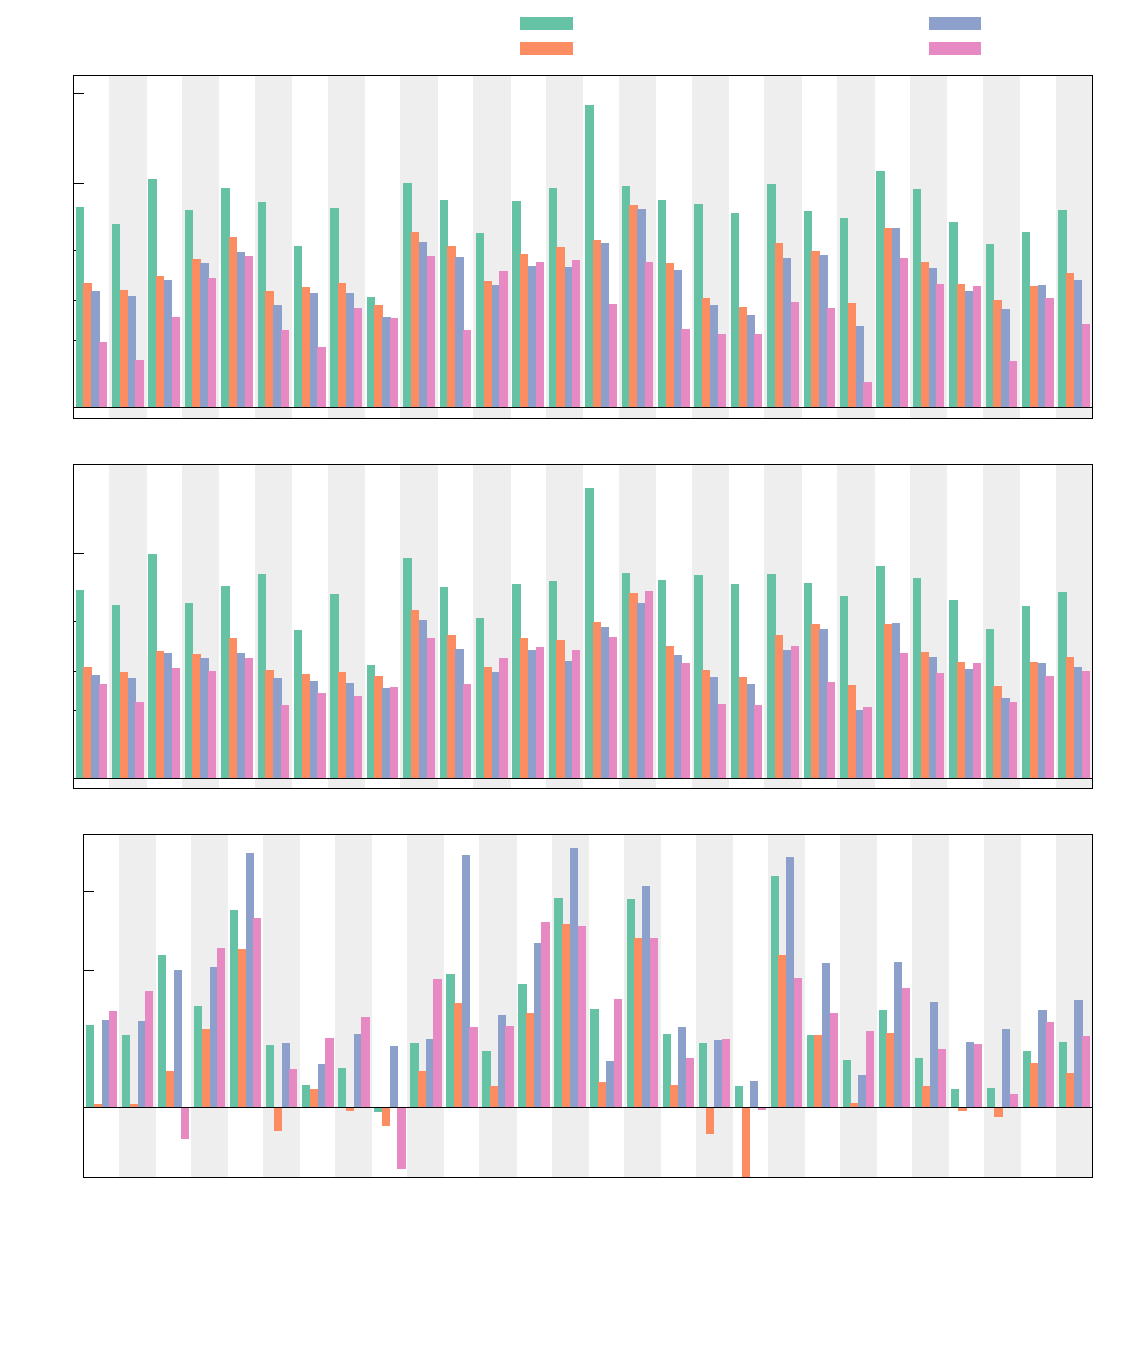
\includegraphics[width={540.00bp},height={360.00bp}]{bar-plot}}%
    \gplfronttext
  \end{picture}%
\endgroup
}
  \caption[Results of simulating and synthesising the PolyBench/C benchmark suite using a range of HLS tools. All figures are relative to Bambu.]{Results of simulating and synthesising the PolyBench/C benchmark suite using a range of HLS tools. All figures are relative to \BambuDefault{}.}%
  \label{fig:list-against-hyper-scheduling}
\end{figure*}

\paragraph{Experimental setup}
Following \textcite{herklotz21_fvhls} and
\textcite{six22_formal_verif_super_sched}, we evaluate our work using
PolyBench/C~\cite{pouchet20_polyb_c}. For each benchmark, the resulting Verilog
hardware design was simulated using Verilator to get the total cycle count. Each
design was synthesised, placed, and routed onto a Xilinx series 7 FPGA (part
number: \mono{xc7z020clg484-1}) using Vivado to get its total area and its
maximum frequency.  We then calculated
$\text{total execution time} = \frac{\text{total clock cycles}}{\text{maximum
    frequency}}$.  We ensured that every design met the timing constraints of a
100MHz clock.

\paragraph{Answering RQ1}
To assess whether adding scheduling to Vericert leads to better hardware designs, \cref{fig:list-against-hyper-scheduling} compares the hardware produced by original Vericert (\VericertBase{}) with that produced when hyperblock scheduling is enabled (\VericertHyper{}). We see that, on average, hyperblock scheduling leads to hardware that requires only 0.46$\times$ the cycle count (middle plot). This is unsurprising given that original Vericert only executed a single instruction per clock cycle. In terms of area (bottom plot), hyperblock scheduling has, on average, a slight increase in area.

\paragraph{Answering RQ2}
Hyperblock scheduling is considerably more complicated to implement and verify than list scheduling, as it requires if-conversion to combine basic blocks into hyperblocks, as well as predicate-aware scheduling. If we omit if-conversion entirely (hence avoiding predication too), we obtain list scheduling as a special case. Does hyperblock scheduling yield enough of a performance improvement over list scheduling to justify its additional complexity?

To answer this, \cref{fig:list-against-hyper-scheduling} measures the hardware produced by Vericert with list scheduling (\VericertList{}). On average, list scheduling leads to hardware that requires 0.51$\times$ the cycle count compared to \VericertBase{}, which is 1.1$\times$ the cycle count compared to \VericertHyper{}. We expect hyperblock scheduling to extend its small lead over list scheduling once the heuristics that guide if-conversion are improved.  In particular, our predictions of the latency of predicated instructions are currently quite conservative to ensure that timing constraints are met; improving these estimates is an active research area~\cite{tan15_mappin_lut_fpgas,rizzi23_iterat_method_mappin_aware_frequen,wang23_mapbuf,ustun20_accur_fpga_hls,zheng14_fast_effec_placem_routin_direc}.

In terms of area, we see that \VericertList{} leads to the smallest hardware designs. This can be attributed to the downstream logic synthesis tool being able to save area by optimising chained operations, such as multiply--accumulate, while not having to handle the predicates that are introduced with \VericertHyper{}.

\paragraph{Answering RQ3}
To assess how \VericertHyper{} fares against unverified HLS tools, we compare it
against the state-of-the-art open-source HLS tool
Bambu~\cite[]{ferrandi21_bambu}. We use Bambu in two modes: one where all
default optimisations are enabled (\BambuDefault{}), and one where as many
optimisations as possible are disabled (\BambuNoOpt{}). Note that several
\enquote{optimisations} are built into Bambu and cannot be disabled, such as
list scheduling and loop flattening.

All the bars in \cref{fig:list-against-hyper-scheduling} are relative to \BambuDefault. The pink bars show \BambuNoOpt. We see that although \VericertHyper{} is well behind \BambuDefault{} (its designs require 3$\times$ the cycle count), it performs comparably to \BambuNoOpt{} (1.04$\times$ the cycle count), which is encouraging because \VericertHyper{} and \BambuNoOpt{} have similar feature sets.

\paragraph{Answering RQ4}
To assess whether \VericertHyper{} has acceptable compilation times, we also
compare it against Bambu.  Compilation times did not deviate for Bambu, all of
them being around 3s mainly due to long startup costs. \VericertHyper{} compiled
each benchmark in 0.9s, also without much variation, showing that verification
was not overly costly.  As for whether our design decisions led to these
compilation times: we remark that if we disable the \enquote{final-state
  predicates} innovation that we introduced in \cref{sec:thirdattempt}, none of
the benchmarks compile within a few minutes and eventually the machine runs out
of memory.

% \Cref{fig:list-against-hyper-scheduling} shows the final results relative to the base version of Vericert.  First, the relative cycle counts between each tool shows that list scheduling has 0.59$\times$ the number of cycles compared to base Vericert and hyperblock scheduling has 0.56$\times$ the number of cycles compared to base Vericert, showing that scheduling instructions provides a large improvement compared to the total number of cycles of base Vericert.  Bambu with optimisations turned-off has around 0.42$\times$ the number of cycles, and with optimisations has 0.14$\times$ the number of cycles, taking drastically fewer cycles.  One outlier here is the jacobi-1d benchmark, where only optimised Bambu finds a way to reduce the number of cycles.  This is because it is a very small benchmark with a single loop, which cannot be optimised by the scheduling algorithms and requires more advanced loop optimisations such as loop pipelining.

% However, looking at the relative execution time is a bit surprising, because on average, the hyperblock scheduling algorithm only performs as well as base Vericert, whereas the list scheduling algorithm performs much better.  This is because the operation chaining heuristics used did not work consistently for the hyperblock scheduling pass, therefore reducing the maximum operating frequency dramatically in some cases.  This is something that needs to be addressed in the heuristics used to perform the if-conversion, but also in the latency constraints in the scheduler.  Interestingly, however, the output of the list scheduling algorithm is around 14\% faster than unoptimised Bambu.  Again, optimised Bambu optimises the benchmarks much further, but also has a slightly higher maximum frequency, bringing the gap down a bit compared to the total cycle counts.

% Finally, looking at area, list scheduling actually also reduces the area
% compared to base Vericert, which is mainly due to the synthesis tool being
% able to optimise chained operations, such as multiply-accumulate operations,
% further.  However, because of the addition of predicates in hyperblock
% scheduling, the area is similar to base Vericert.  This area is similar to
% unoptimised Bambu, however, optimised Bambu achieves 0.6$\times$ the area.

%%% Local Variables:
%%% mode: latex
%%% TeX-master: "../thesis"
%%% TeX-engine: luatex
%%% End:


\chapter{Conclusion}%
\label{sec:conclusion}

\section{Limitations and Future Work}

There are various limitations in \vericert{} compared to other HLS tools due to the fact that our main focus was on formally verifying the translation from 3AC to Verilog. In this section, we outline the current limitations of our tool and suggest how they can be overcome in future work, first describing limitations to the generated hardware, and then describing the limitations on the software input that \vericert{} accepts.

%\NR{You have very different types of limitations. I wonder if grouped them into software and hardware limitations respectively might simplify this section. Just a suggestion.}

\subsection{Limitations to the Generated Hardware}

%This section describes the current limitations and possible improvements that could be made to the generated hardware.

\paragraph{Lack of instruction-level parallelism}

%\JW{I'm hesitant about this paragraph. Yes, we have to write something about how future-proof Vericert is, as this is required by the reviewers and promised in our list of changes. But I worry that if we place too much emphasis on how straightforward it will be to add scheduling, then we'll make it harder for ourselves to publish a paper about adding scheduling (``But you said in your OOPSLA 2021 paper that this was all straightforward'' etc.) In what follows, I've tried to strike a balance -- see what you think.}\YH{Yeah I think I like the paragraph and the balance in it, I think it still explains that existing passes should not have to change.  I think reviewer 2 wanted a detailed explanation of this, but I do agree that it should not be needed in this paper.}
The main limitation of \vericert{} is that it does not perform instruction scheduling, which means that instructions cannot be gathered into the same state and executed in parallel.
%This limitation is present by design so that the focus could be made on the initial proof of correctness of the translation of instructions with a sequential schedule.
However, each language in \vericert{} was designed with scheduling in mind, so that these should not have to change fundamentally when that is implemented in the future.
For instance, our HTL language already allows arbitrary Verilog to appear in each state of the FSMD; currently, each state just contains a single Verilog assignment, but when scheduling is added, it will contain a list of assignments that can all be executed in parallel. We expect to follow the lead of \textcite{tristan08_formal_verif_trans_valid} and \textcite{six+20}, who have previously added scheduling support to CompCert in a VLIW context, by invoking an external (unverified) scheduling tool and then using translation validation to verify that each generated schedule is correct (as opposed to verifying the scheduling tool itself).
%The translation from 3ACPar to HTL would not change conceptually, except for the fact that multiple instructions can now be translated into the same state.
%This means that the proof of translation from 3AC to HTL can also be adapted with minimal changes to the top-level of the proofs.
%The bulk of the proofs proving the translation of single instructions would stay intact.

%However, the design of the intermediate languages in \vericert{} take this optimisation into account and are designed to support scheduling in the future.

%\NRIt is best to explain why we didn't focus on scheduling with a positive/future work spin. For example, ``It was more intuitive to handle one instruction per cycle at the initial stage of our project as we want to focus our efforts on correctness, which has been the main weakness of HLS, rather than performance. However, we were very much aware during the design stage that in order for our compiler to be able to perform better, supporting of scheduling was inevitable. Hence, we intentionally left room for support of scheduling. In essence, instead of supporting one instruction per cycle, we must be able to support a list of instructions per cycle. To do so, we envision extensions to our work in several ways.'' We might not even need to specify the details of how. You can keep the tricks in your sleeves for the next publication. \YH{Well one of the only things the reviewers wanted us to add was a realistic implementation of scheduling, so I think we need to at least keep that.}.

%To simplify the proof of the scheduling algorithm, and to minimise the changes necessary for the current translation from 3AC to HTL, a new language must be introduced, called 3ACPar, which would be equivalent to 3AC but instead of consisting of a map from program counter to instruction, it would consist of a map from program counter to list of instructions, which can all be executed in parallel.  A new proof for the scheduling algorithm would have to be written for the translation from 3AC to 3ACPar, for which a verified translation validation approach might be appropriate, however, the translation form 3ACPar to HTL would not change conceptually, except for the fact that multiple instructions can now be translated into the same state.  This small difference means that most of the proof can be reused without any changes, as the translation of instructions was the main body of the proof and did not change.

\paragraph{Lack of pipelined division}
Pipelined operators can execute different stages of an operation in parallel, and thus perform several long-running operations simultaneously while sharing the same hardware.
The introduction of pipelined operators to \vericert{}, especially for division, would alleviate the slow clock speed observed in the \polybench{} benchmarks when divisions were included (Fig.~\ref{fig:polybench-div}). In HTL, pipelined operations could be represented in a similar fashion to load and store instructions, by using wires to communicate with an abstract computation block modelled in HTL and later replaced by a hardware implementation.
%\NR{Are you describing using IP blocks? If so, you can generalise it to any IP block rather than just division.}\YH{I think I prefer just focusing on pipelined division for now, as that's specifically the issue, so that people know we have a plan to resolve specifically that.}
%JW I've chopped the following sentence because it felt like it was going into too much detail.
%However, 3ACPar would have to be modified to also describe such instructions so that these can be placed optimally using the external scheduling algorithm.

\subsection{Limitations on the Software Input}

%This section describes the limitations and possible improvements to the software input accepted by \vericert{}.

\paragraph{Limitations with I/O}

\vericert{} is currently limited in terms of I/O because the main function cannot accept any arguments if the Clight program is to be well-formed.\footnote{Technically, \vericert{} (and indeed, \compcert{}) can compile main functions that have arbitrary arguments and will handle those inputs appropriately, but the correctness theorem offers no guarantees about such programs.} Moreover, external function calls that produce traces have not been implemented yet, but these could enable the C program to read and write values on a bus that is shared with various other components in the hardware design.

\paragraph{Lack of support for global variables}
In \compcert{}, each global variable is stored in its own memory.  A generalisation of our translation of the stack into a RAM block could therefore translate global variables in the same manner.  This would require a slight generalisation of pointers so that they store provenance information to ensure that each pointer accesses the right RAM. It would also be necessary to generalise the RAM interface so that it decodes the provenance information and indexes the correct array.
%\NR{Curiously, is memory analysis in your to-do list?}\YH{Well kind of, would be nice, but probably not sophisticated analysis.}

\paragraph{Other language restrictions}
C and Verilog handle signedness quite differently. By default, all operators and registers in Verilog (and HTL) are unsigned, so to force an operation to handle the bits as signed, both operators have to be forced to be signed. Moreover, Verilog implicitly resizes expressions to the largest needed size by default, which can affect the result of the computation.  This feature is not supported by the Verilog semantics we adopted, so to match the semantics to the behaviour of the simulator and synthesis tool, braces are placed around all expressions to inhibit implicit resizing.  Instead, explicit resizing is used in the semantics, and operations can only be performed on two registers that have the same size.

Furthermore, equality checks between \emph{unsigned} variables are actually not supported, because this requires supporting the comparison of pointers, which should only be performed between pointers with the same provenance.  In \vericert{} there is currently no way to determine the provenance of a pointer, and it therefore cannot model the semantics of unsigned comparison in \compcert{}. This is not a severe restriction in practice however, because in the absence of dynamic allocation, equality comparison of pointers is rarely needed, and equality comparison of integers can still be performed by casting them both to signed integers.

Finally, the \texttt{mulhs} and \texttt{mulhu} instructions, which fetch the
upper bits of a 32-bit multiplication, are not translated by \vericert{},
because 64-bit numbers are not supported. These instructions are only generated
to optimise divisions by a constant that is not a power of two, so turning off
constant propagation will allow these programs to pass without error.

\subsection{Coq Mechanisation}

\begin{table}
  \centering
  \caption{Statistics about the numbers of lines of code in the proof and implementation of \vericert{}.}\label{tab:proof_statistics}
  \begin{tabular}{lrrrrr}
    \toprule
    & \textbf{Coq code} & \multicolumn{1}{p{1cm}}{\raggedleft\textbf{OCaml code}} & \textbf{Spec} & \multicolumn{1}{p{2cm}}{\raggedleft\textbf{Theorems \& Proofs}} & \textbf{Total}\\
    \midrule
    {Data structures and libraries}     & 280  & --- & ---  & 500  & 780   \\
    {Integers and values}               & 98   & --- & 15   & 968  & 1081  \\
    {HTL semantics}                     & 50   & --- & 181  & 65   & 296   \\
    {HTL generation}                    & 590  & --- & 66   & 3069 & 3725  \\
    {RAM generation}                    & 253  & --- & ---  & 2793 & 3046  \\
    {Verilog semantics}                 & 78   & --- & 431  & 235  & 744   \\
    {Verilog generation}                & 104  & --- & ---  & 486  & 590   \\
    {Top-level driver, pretty printers} & 318  & 775 & ---  & 189  & 1282  \\
    \midrule
    \textbf{Total}                      & 1721 & 775 & 693  & 8355 & 11544 \\
    \bottomrule
  \end{tabular}
\end{table}

The lines of code for the implementation and proof of \vericert{} can be found
in Table~\ref{tab:proof_statistics}.  Overall, it took about 1.5 person-years to
build \vericert{} -- about three person-months on implementation and 15
person-months on proofs.  The largest proof is the correctness proof for the HTL
generation, which required equivalence proofs between all integer operations
supported by \compcert{} and those supported in hardware.  From the 3069 lines
of proof code in the HTL generation, 1189 are for the correctness proof of just
the load and store instructions.  These were tedious to prove correct because of
the substantial difference between the memory models used, and the need to prove
properties such as stores outside of the allocated memory being undefined, so
that a finite array could be used. In addition to that, since pointers in HTL
and Verilog are represented as integers, instead of as a separate `pointer' type
like in the \compcert{} semantics, it was painful to reason about them.  Many
new theorems had to be proven about them in \vericert{} to prove the conversion
from pointer to integer.  Moreover, the second-largest proof of the correct RAM
generation includes many proofs about the extensional equality of array
operations, such as merging arrays with different assignments.  As the negative
edge implies that two merges take place every clock cycle, the proofs about the
equality of the contents in memory and in the merged arrays become more tedious
too.

Looking at the trusted computing base of \vericert{}, the Verilog semantics is
431 lines of code.  This and the Clight semantics from \compcert{} are the only
parts of the compiler that need to be trusted.  The Verilog semantics
specification is therefore much smaller compared to the 1721 lines of the
implementation that are written in Coq, which are the verified parts of the HLS
tool, even when the Clight semantics are added.  In addition to that,
understanding the semantics specification is simpler than trying to understand
the translation algorithm. We conclude that the trusted base has been
successfully reduced.

%%% Local Variables:
%%% mode: latex
%%% TeX-master: "../thesis"
%%% TeX-engine: luatex
%%% End:


\begingroup
\singlespacing
\printbibliography

\printglossary[type=index,style=bookindex]
\endgroup

\end{document}

%%% Local Variables:
%%% mode: latex
%%% TeX-master: t
%%% TeX-engine: luatex
%%% End:
